%%%%%%%%%%%%%%%%%%%%%%%%%%%%%%%%%%%%%%%%%%%%%%%%%%%%%%%%%%%%%%%%%%%%%%%%%%%%%%%%
% PREAMBLE
%%%%%%%%%%%%%%%%%%%%%%%%%%%%%%%%%%%%%%%%%%%%%%%%%%%%%%%%%%%%%%%%%%%%%%%%%%%%%%%%
\documentclass[11pt]{article}

% --- Packages for Page Layout and Encoding ---
\usepackage[utf8]{inputenc}
\usepackage[T1]{fontenc}
\usepackage[a4paper, margin=1in]{geometry}

% --- Packages for Graphics and Color ---
\usepackage{graphicx}
\usepackage{xcolor}
\usepackage{subcaption} % For subfigures
\usepackage{placeins}   % Provides \FloatBarrier

% --- Packages for Tables ---
\usepackage{longtable}
\usepackage{booktabs} % For professional-looking tables (\toprule, \midrule, \bottomrule)
\usepackage{tabularx}
\usepackage{ltablex} % Fixes interaction between longtable and tabularx

% --- Packages for Mathematics and Physics ---
\usepackage{amsmath}
\usepackage{amssymb}
\usepackage{braket}
%\usepackage{siunitx} % For typesetting units and numbers, e.g., \SI{120}{\giga\electronvolt}

% --- Packages for Document Structure and References ---
\usepackage[hidelinks]{hyperref} % For clickable links
\usepackage{authblk}           % For author affiliations
\usepackage{lineno}            % For line numbers
%\linenumbers

% --- Custom Commands and Settings ---
\newcommand{\dyprocess}{\text{p+p} \rightarrow \mu^+\mu^-X}
\newcommand{\diffd}{\mathrm{d}}
\renewcommand{\Authand}{, } % Adjusts authblk separator
%\sisetup{per-mode=symbol} % Uses '/' for units like GeV/c^2

% Fix for "Counter too large" error with many subfigures
\usepackage{chngcntr}
\counterwithout{figure}{section}
\counterwithout{table}{section}

%%%%%%%%%%%%%%%%%%%%%%%%%%%%%%%%%%%%%%%%%%%%%%%%%%%%%%%%%%%%%%%%%%%%%%%%%%%%%%%%
% DOCUMENT START
%%%%%%%%%%%%%%%%%%%%%%%%%%%%%%%%%%%%%%%%%%%%%%%%%%%%%%%%%%%%%%%%%%%%%%%%%%%%%%%%
\begin{document}
\linenumbers
% --- Title Block ---
\title{\textbf{Measurement of the Drell-Yan Absolute Cross-Section in $pp$ Collisions with a 120 GeV Proton Beam at Fermilab}}
\author[1]{Chatura Kuruppu}
\author[1]{Stephen Pate}
\affil[1]{New Mexico State University, Las Cruces, NM 88003, USA}
\date{October 2, 2025}
\maketitle

% --- Abstract ---
\begin{abstract}
This analysis note reports on the determination of $pp$ Drell-Yan absolute cross sections from data collected using the Roadset 67 trigger.
We seek preliminary approval of these results, for presentation in upcoming conferences.  Similar techniques will be used to determine the $pd$ DY cross section, and then we will move on to include data from the other run 2-3 and 5-6 roadsets.
%The proton-induced Drell-Yan process is a powerful experimental tool for probing the antiquark distributions within nucleons. While existing data have extensively covered the region of small parton momentum fraction ($x$), the SeaQuest experiment at Fermilab extends the kinematic reach to larger $x$ values by utilizing a 120 GeV proton beam. In this work, we report the measurement of the double-differential Drell-Yan cross-sections, $\diffd^{2}\sigma/\diffd x_{F}\diffd M$, from collisions of protons with both liquid deuterium (p+d) and liquid hydrogen (p+p) targets. These measurements provide direct sensitivity to the $\bar{u}(x) + \bar{d}(x)$ and $\bar{u}(x)$ antiquark distributions of the proton, respectively. The results are compared with theoretical predictions from Quantum Chromodynamics (QCD) using several current parameterizations of the proton's parton distribution functions. Additionally, these new data are compared with previous measurements to examine the scaling behavior of the Drell-Yan cross-section across a broad range of the kinematic variable $\sqrt{\tau}$.
\vspace{1em}
\hrule
\vspace{1em}
\footnotesize{This work was supported in part by US DOE grant DE-FG02-94ER40847.}
\end{abstract}

\clearpage

% --- Table of Contents, List of Figures, List of Tables ---
\tableofcontents
\clearpage
\listoffigures
\clearpage
\listoftables
\clearpage

% --- Sections (Content remains the same, only structural fixes applied) ---

\section{Introduction}
\label{sec:introduction}
The Drell-Yan process, where a quark from one hadron annihilates with an antiquark from another to produce a lepton-antilepton pair ($q\bar{q} \rightarrow \ell^+\ell^-$), provides a clean and direct probe of the antiquark structure of nucleons. Over the past several decades, Drell-Yan experiments have been instrumental in mapping the parton distribution functions (PDFs) of the proton and other hadrons. However, most existing data are concentrated at small to moderate values of the parton momentum fraction, $x < 0.3$. The region of large $x$ ($x>0.3$) remains relatively unexplored, yet it is crucial for understanding phenomena such as the flavor asymmetry of the proton's light antiquark sea ($\bar{d}(x)/\bar{u}(x)$) and the fundamental mechanisms of non-perturbative QCD that govern hadron structure.

The SeaQuest experiment (E906) at Fermilab was designed specifically to explore this high-$x$ frontier. By impinging a high-intensity 120 GeV proton beam from the Main Injector onto various fixed targets, including liquid hydrogen (LH$_2$) and liquid deuterium (LD$_2$), SeaQuest measures dimuon production in a kinematic region sensitive to antiquarks carrying a large fraction of the nucleon's momentum.

This analysis presents a measurement of the absolute double-differential Drell-Yan cross-section, binned in the dimuon invariant mass ($M$) and Feynman-$x$ ($x_F$), using data collected with the LH$_2$ and LD$_2$ targets. The p+p collisions are primarily sensitive to the $\bar{u}$ distribution in the proton, while the p+d collisions provide information on the sum of $\bar{u}$ and $\bar{d}$. These results provide stringent new constraints on modern PDF parameterizations in the valence-dominated region.

The cross-section is presented in its scaling form, which, in the leading-order Drell-Yan model, is independent of the center-of-mass energy, $\sqrt{s}$:
\begin{equation}
    M^{3}\frac{\diffd^{2}\sigma}{\diffd M \diffd x_{F}} = f(\tau)
\end{equation}
where $\tau = M^2/s$. The experimental determination of this quantity requires a precise understanding of the integrated luminosity, detector acceptance, and reconstruction efficiencies, which are detailed in the subsequent sections of this document.

\section{Analysis Methodology}
\label{sec:methodology}
The extraction of the Drell-Yan cross-section from the raw data involves several distinct steps: selecting candidate dimuon events, subtracting backgrounds, calculating the integrated luminosity, and correcting for detector- and reconstruction-related inefficiencies.

\subsection{Data and Monte Carlo Samples}
This analysis utilizes the ``Roadset 67'' dataset collected by the SeaQuest experiment. The primary data files for the liquid hydrogen (LH$_2$) target and the corresponding empty "flask" target runs are saved in:
\begin{verbatim}
    /seaquest/users/apun/e906_projects/rs67_merged_files/
\end{verbatim}
\begin{itemize}
    \item \textbf{Data (LH$_2$ Target):} \texttt{merged\_RS67\_3089LH2.root}
    \item \textbf{Background (Empty Flask):} \texttt{merged\_RS67\_3089Flask.root}
\end{itemize}
The empty flask data are crucial for subtracting contributions from beam interactions with the target vessel walls and other upstream material.

To correct for detector acceptance and reconstruction efficiencies, extensive Monte Carlo (MC) simulations were employed. The simulations model the Drell-Yan process and propagate the resulting muons through a Geant4-based model of the SeaQuest spectrometer. The primary MC files used are:
\begin{itemize}
    \item \textbf{Acceptance Study:} Drell-Yan events were generated over a $4\pi$ solid angle ("thrown") and also processed through the full detector simulation and reconstruction chain ("accepted"). This study uses the \texttt{*\_M027\_S001\_*} series of files saved in: \begin{verbatim}
        /seaquest/users/chleung/pT_ReWeight/
    \end{verbatim}
    \begin{itemize}
        \item \textbf{mc\_drellyan\_LH2\_M027\_S001\_4pi\_pTxFweight\_v2.root}
	    \item \textbf{mc\_drellyan\_LH2\_M027\_S001\_clean\_occ\_pTxFweight\_v2.root}
	    \item \textbf{mc\_drellyan\_LH2\_M027\_S001\_messy\_occ\_pTxFweight\_v2.root}
        \item \textbf{mc\_drellyan\_LD2\_M027\_S001\_4pi\_pTxFweight\_v2.root}
        \item \textbf{mc\_drellyan\_LD2\_M027\_S001\_clean\_occ\_pTxFweight\_v2.root}
        \item \textbf{mc\_drellyan\_LD2\_M027\_S001\_messy\_occ\_pTxFweight\_v2.root}
    \end{itemize}
    \item \textbf{Efficiency Study:} To model the effect of high detector occupancy on track reconstruction, simulated events were processed with ("messy") and without ("clean") the overlay of random background hits from experimental data. This study uses the \texttt{*\_M027\_S002\_*} series of files also saved in the same location:
    \begin{itemize}
        \item \textbf{mc\_drellyan\_LH2\_M027\_S002\_clean\_occ\_pTxFweight\_v2.root}
        \item \textbf{mc\_drellyan\_LH2\_M027\_S002\_messy\_occ\_pTxFweight\_v2.root}    
    \end{itemize}
\end{itemize}
All MC samples are weighted on an event-by-event basis to match the transverse momentum ($p_T$) distribution observed in the data.

\subsection{Event Selection}
\label{sec:event_selection}
A multi-tiered set of selection criteria is applied to isolate high-quality Drell-Yan dimuon events from the large background of other processes.
\begin{itemize}
    \item \textbf{Data Quality:} Only data from "good spills," as identified by standard run quality monitoring, are included in the analysis. A physics trigger condition (\texttt{MATRIX1 == 1}) is required, selecting events consistent with the passage of two muons through the spectrometer.
    \item \textbf{Track and Dimuon Quality:} A set of stringent cuts, developed by the collaboration and referred to as "Chuck cuts," are applied to ensure well-reconstructed positive and negative muon tracks that form a high-quality common vertex. These cuts impose requirements on track $\chi^2$, momentum, number of hits, and fiducial volume. The full details of these cuts are provided in Appendix \ref{app:event_selection}.
    \item \textbf{Kinematic Selection:} The analysis focuses on the high-mass continuum, away from the charmonium resonances ($J/\psi, \psi'$). A cut of $M_{\mu\mu} > 4.2$ GeV is applied. The analysis is restricted to the kinematic range $0 < x_F < 0.8$.
\end{itemize}

\subsection{Cross-Section Formalism}
The double-differential cross-section in a given kinematic bin ($\Delta M, \Delta x_F$) is calculated as:
\begin{equation}
\frac{\diffd^{2}\sigma}{\diffd M \diffd x_{F}} = \frac{N_{DY}}{\Delta M \Delta x_{F} \cdot \mathcal{L} \cdot \epsilon_{\text{total}}}
\label{eq:modified_cross_section}
\end{equation}
where:
\begin{itemize}
    \item $N_{DY}$ is the number of Drell-Yan events in the bin after subtraction of the combinatoric and empty flask backgrounds (see \cite{alternativeDY} DocDB 11322).
    $$N_{DY} = N_{\rm LH2}-N_{\rm LH2,~mixed} - \frac{I_{\rm LH2}}{I_{\rm flask}}\left( N_{\rm flask}-N_{\rm flask,~mixed}\right)$$
    \item $\mathcal{L}$ is the integrated luminosity for the dataset.
    \item $\epsilon_{\text{total}}$ is the total correction factor, accounting for acceptance and inefficiencies.
\end{itemize}
The integrated luminosity, $\mathcal{L}$, is given by the product of the total number of protons incident on the target and the number of target nuclei per unit area:
\begin{equation}
\mathcal{L} = N_{\text{incident}} \cdot \frac{N_{A} \rho L}{A} \cdot f_{\text{atten}}
\label{eq:luminosity}
\end{equation}
Here, $N_{\text{incident}}$ is the number of protons on target, $N_A$ is Avogadro's number, $\rho$ is the target density, $L$ is the target length, $A$ is the molar mass, and $f_{\text{atten}}$ is a correction factor for beam attenuation within the thick target. For the $L=50.8$ cm long LH$_2$ target, with a density of $\rho_H=0.0708$~g/cm$^3$, the target thickness is 3.5966 g/cm$^2$ with a beam attenuation factor of 0.966.

The total correction factor, $\epsilon_{\text{total}}$, is the product of three terms determined from MC simulations:
\begin{equation}
\epsilon_{\text{total}} = \epsilon_{\text{acc}}(M,x_{F}) \cdot \epsilon_{\text{recon}}(M,x_{F}) \cdot \epsilon_{\text{trigger}}
\end{equation}
where $\epsilon_{\text{acc}}$ is the geometric and kinematic acceptance of the spectrometer, $\epsilon_{\text{recon}}$ is the track reconstruction efficiency (often called "kTracker efficiency"), and $\epsilon_{\text{trigger}}$ is the trigger efficiency. The calculation of these three terms is detailed in the following sections.

\section{Acceptance and Efficiency Corrections}
\label{sec:corrections}

\subsection{Detector Acceptance Correction}
The SeaQuest spectrometer has a finite geometric acceptance, which limits the fraction of produced dimuon events that can be detected. This acceptance depends strongly on the event kinematics, primarily the dimuon invariant mass ($M$) and Feynman-$x$ ($x_F$). The acceptance correction factor is determined using MC simulations.

The acceptance, $A(M, x_F)$, is defined as the ratio of the number of simulated events that are successfully reconstructed and pass all analysis cuts ($N_{\text{reco}}$) to the total number of events generated in a given kinematic bin ($N_{\text{gen}}$):
\begin{equation}
\text{Acceptance (A)} = \frac{N_{\text{reco}}}{N_{\text{gen}}}
\label{eq:acceptance}
\end{equation}
This calculation is performed in bins of $M$ and $x_F$. The kinematic binning used for this study is defined by the following edges:
\begin{itemize}
    \item \textbf{$x_F$ Edges}: $\{0, 0.05, 0.1, \dots, 0.8\}$ (16 bins)
    \item \textbf{Mass Edges (GeV/$c^2$)}: $\{4.2, 4.5, 4.8, 5.1, 5.4, 5.7, 6, 6.3, 6.6, 6.9, 7.5, 8.7\}$ (11 bins)
\end{itemize}

The following pages show the calculated acceptance as a function of mass for each of the 16 $x_F$ bins. The plots show the acceptance for the LH$_2$ and LD$_2$ targets, their combined average, and their ratio. The ratio is close to unity across the kinematic range, indicating that target-dependent effects on the acceptance are small. In this case, we compare newly calculated acceptance corrections to the existing acceptance calculations saved in Shivangi's file:
\begin{verbatim}
./shivangi/work/analysis/R008/diffCross/v42/5770/looseCut/final/acceptance_h.root
\end{verbatim}

%--- All Acceptance plots ---
\begin{figure}[p]
    \centering
    \begin{subfigure}[b]{0.48\textwidth}
       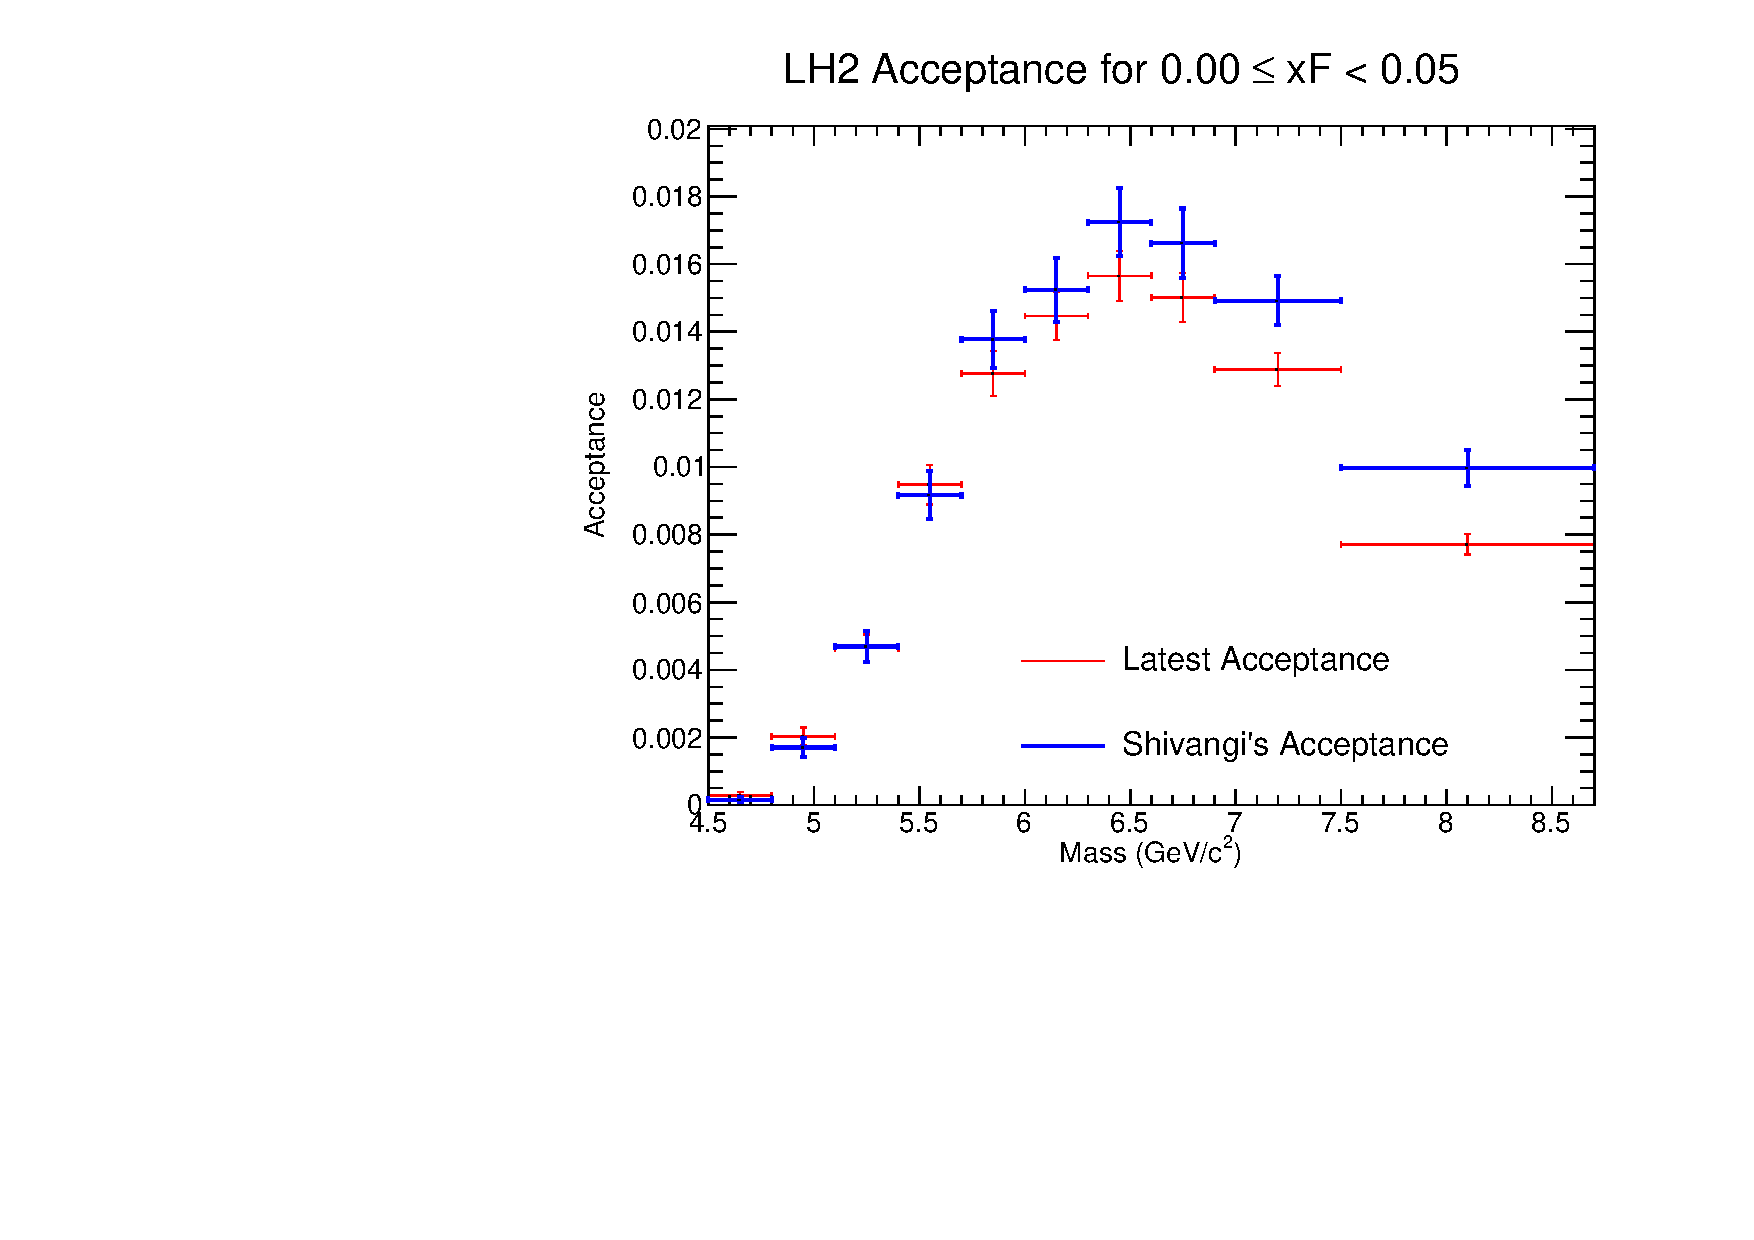
\includegraphics[width=\linewidth]{./acceptancePlots/LH2_acceptance_xF_bin_0.pdf}
       \caption{Acceptance for LH2}
    \end{subfigure}\hfill
    \begin{subfigure}[b]{0.48\textwidth}
       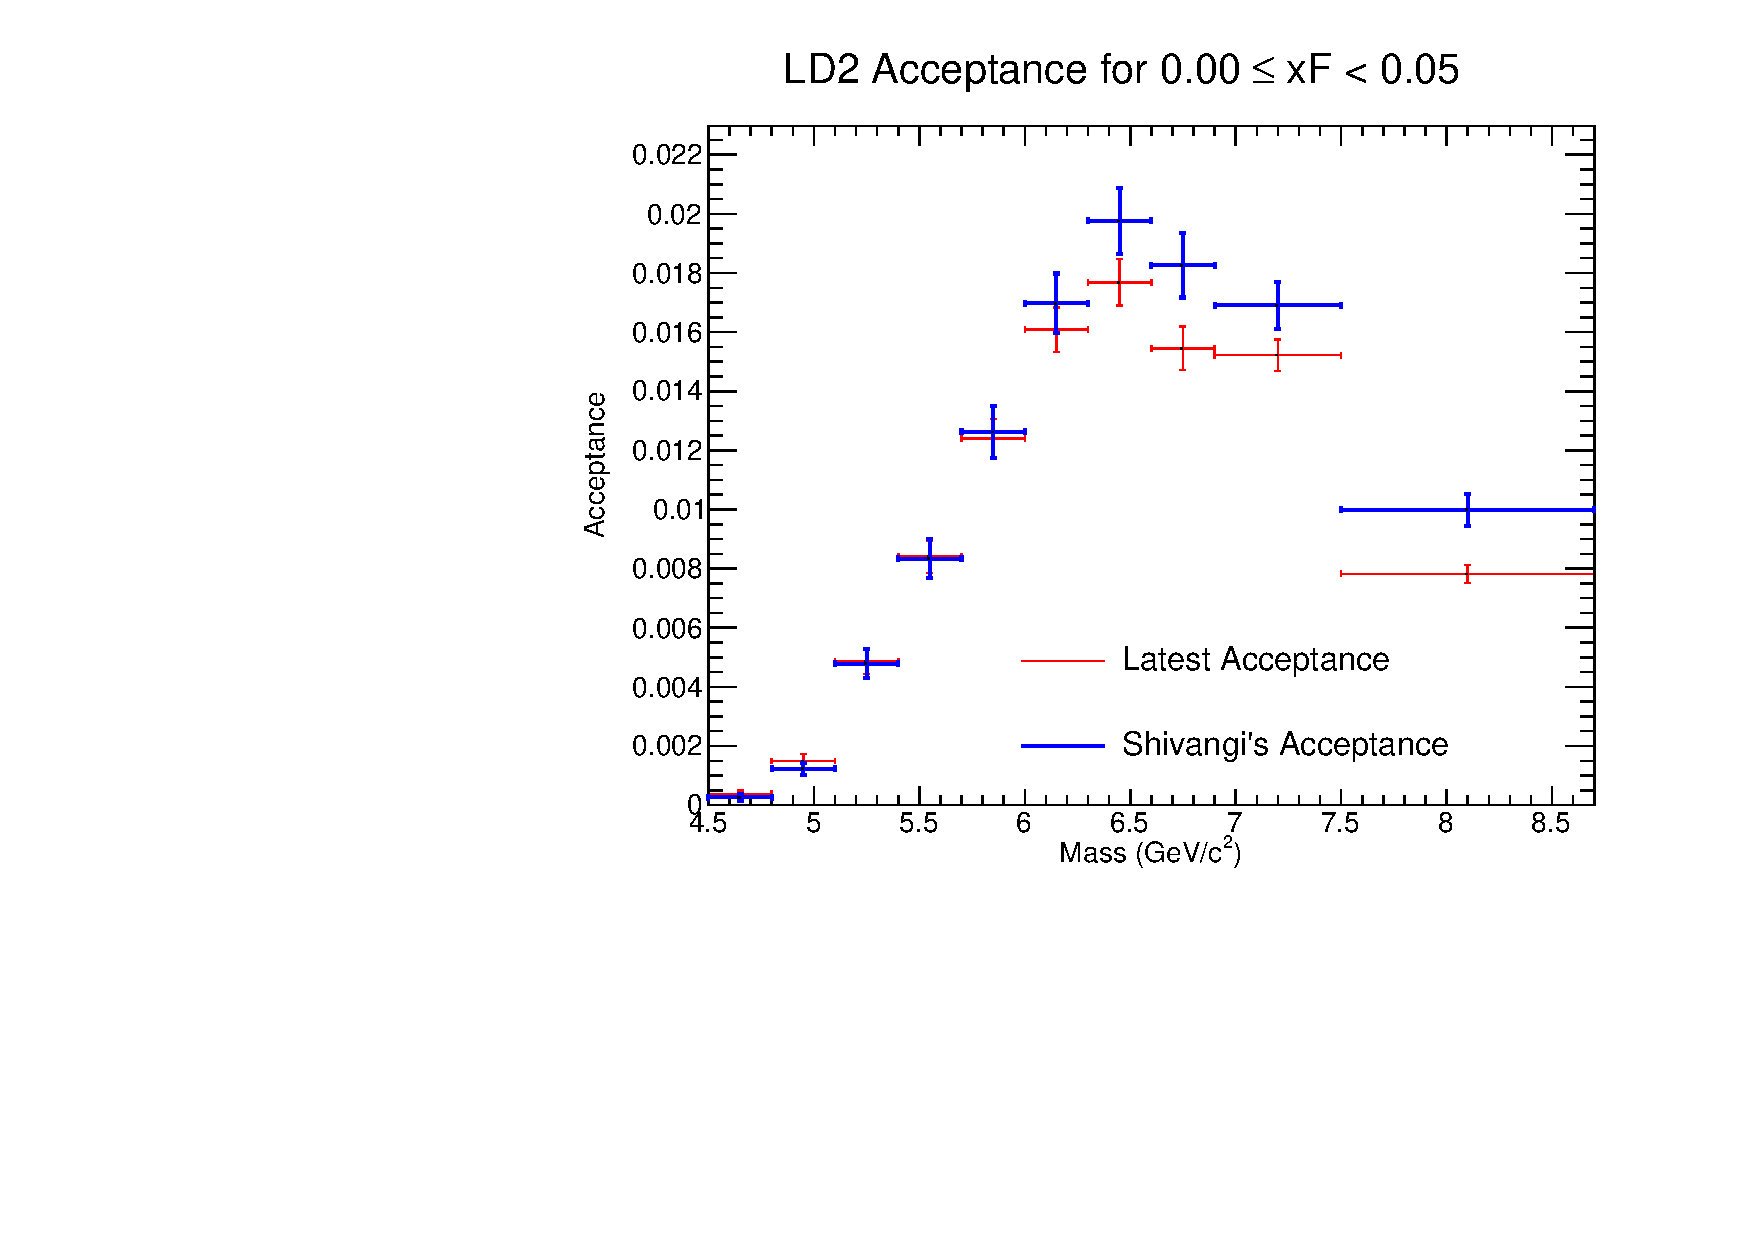
\includegraphics[width=\linewidth]{./acceptancePlots/LD2_acceptance_xF_bin_0.pdf}
       \caption{Acceptance for LD2}
    \end{subfigure}
    \begin{subfigure}[b]{0.48\textwidth}
       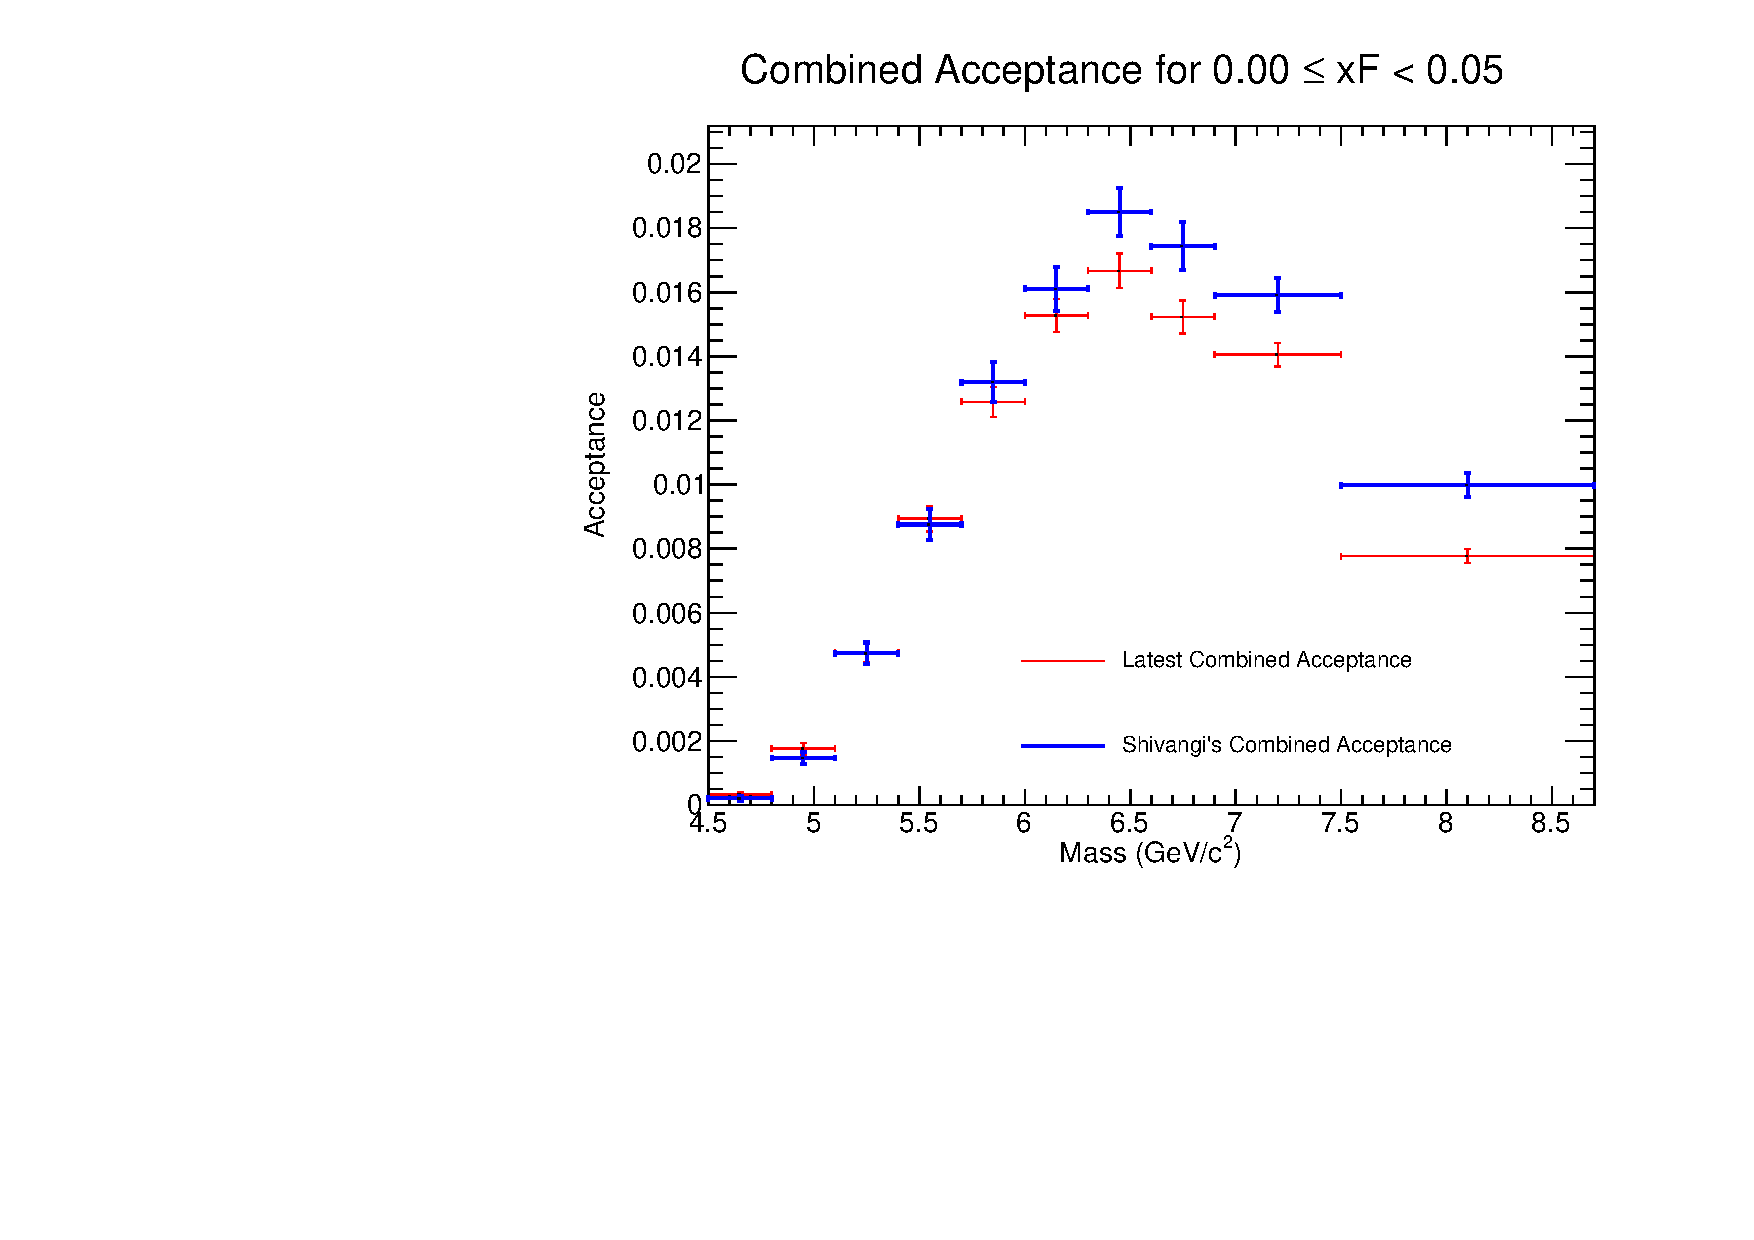
\includegraphics[width=\linewidth]{./acceptancePlots/Combined_acceptance_xF_bin_0.pdf}
       \caption{Combined Acceptance}
    \end{subfigure}\hfill
    \begin{subfigure}[b]{0.48\textwidth}
       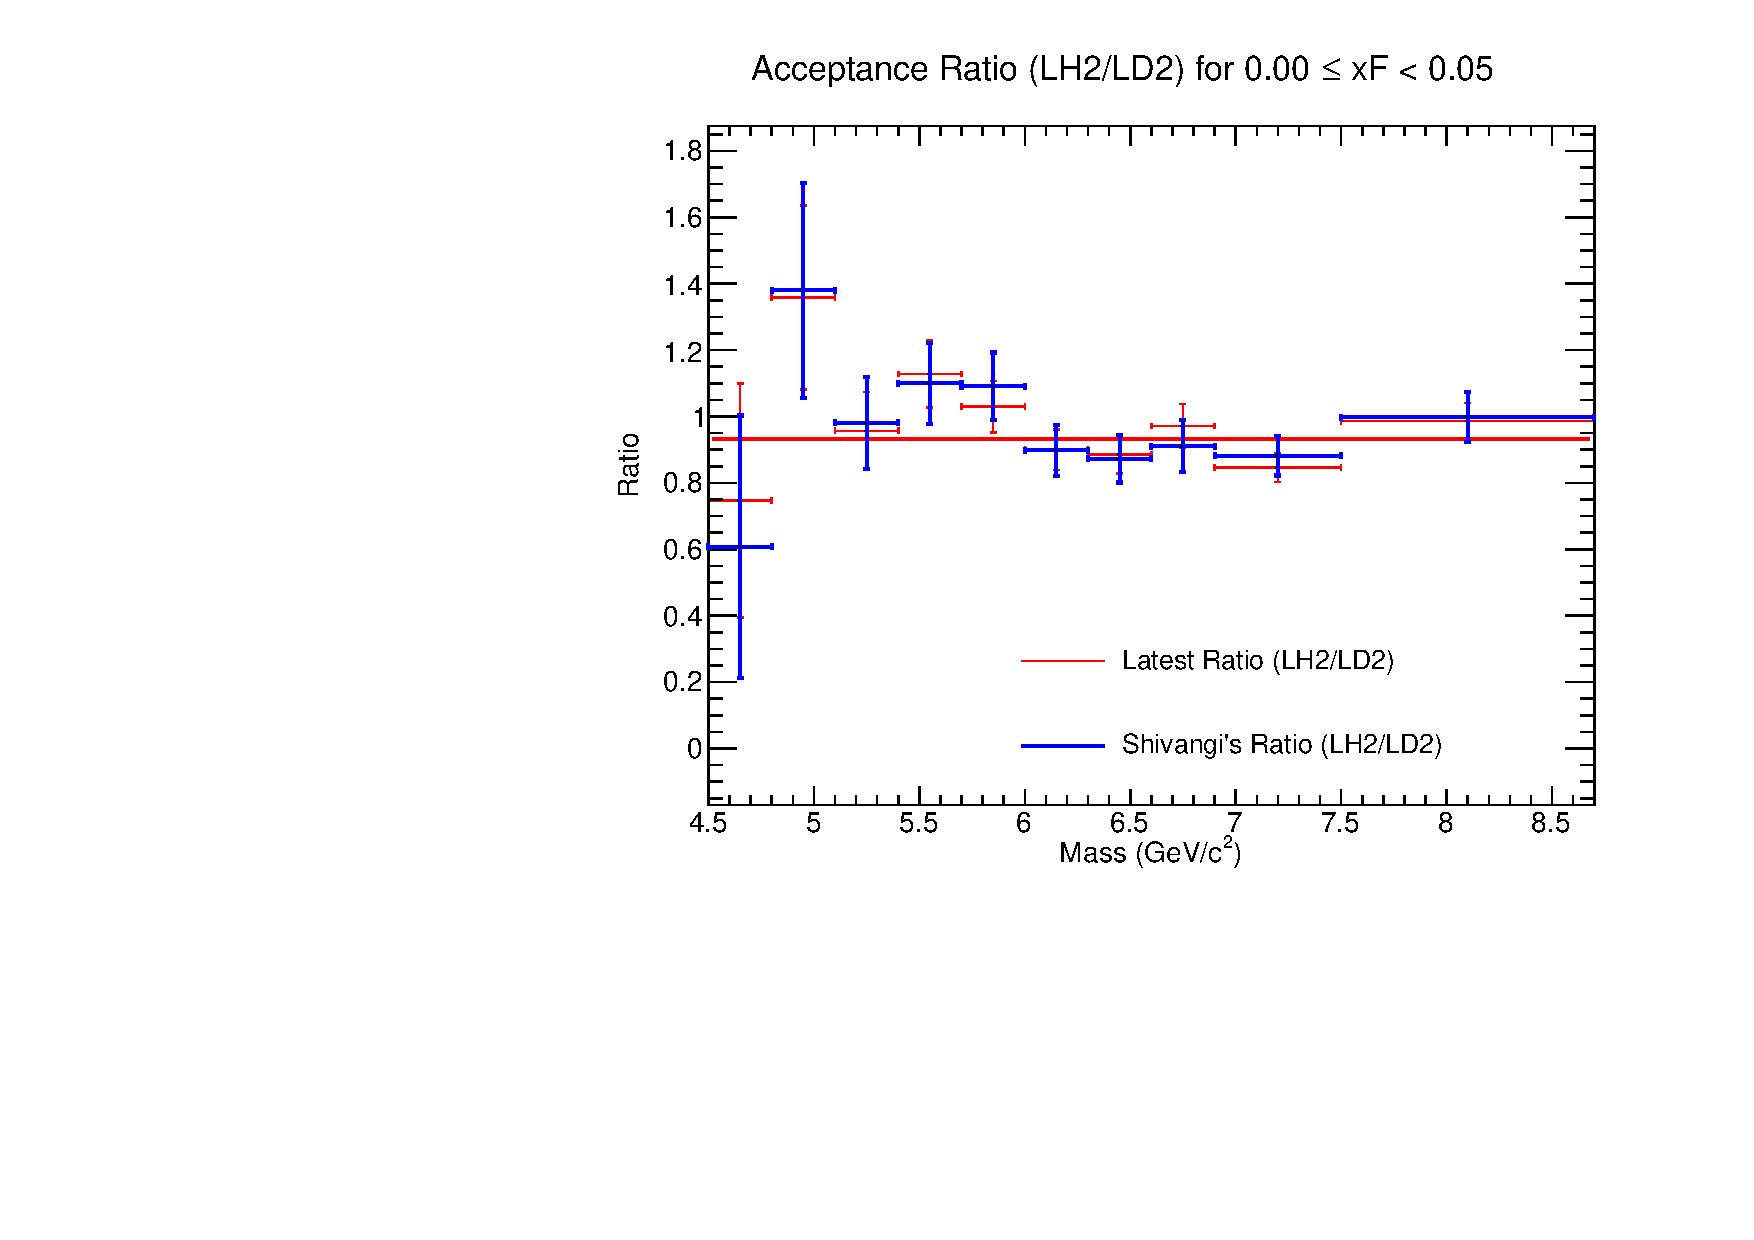
\includegraphics[width=\linewidth]{./acceptancePlots/Acceptance_ratio_xF_bin_0.pdf}
       \caption{Acceptance Ratio (LH2/LD2)}
    \end{subfigure}
    \caption{Acceptance plots for $0.00 \le x_F < 0.05$.}
\end{figure}

\begin{figure}[p]
    \centering
    \begin{subfigure}[b]{0.48\textwidth}
       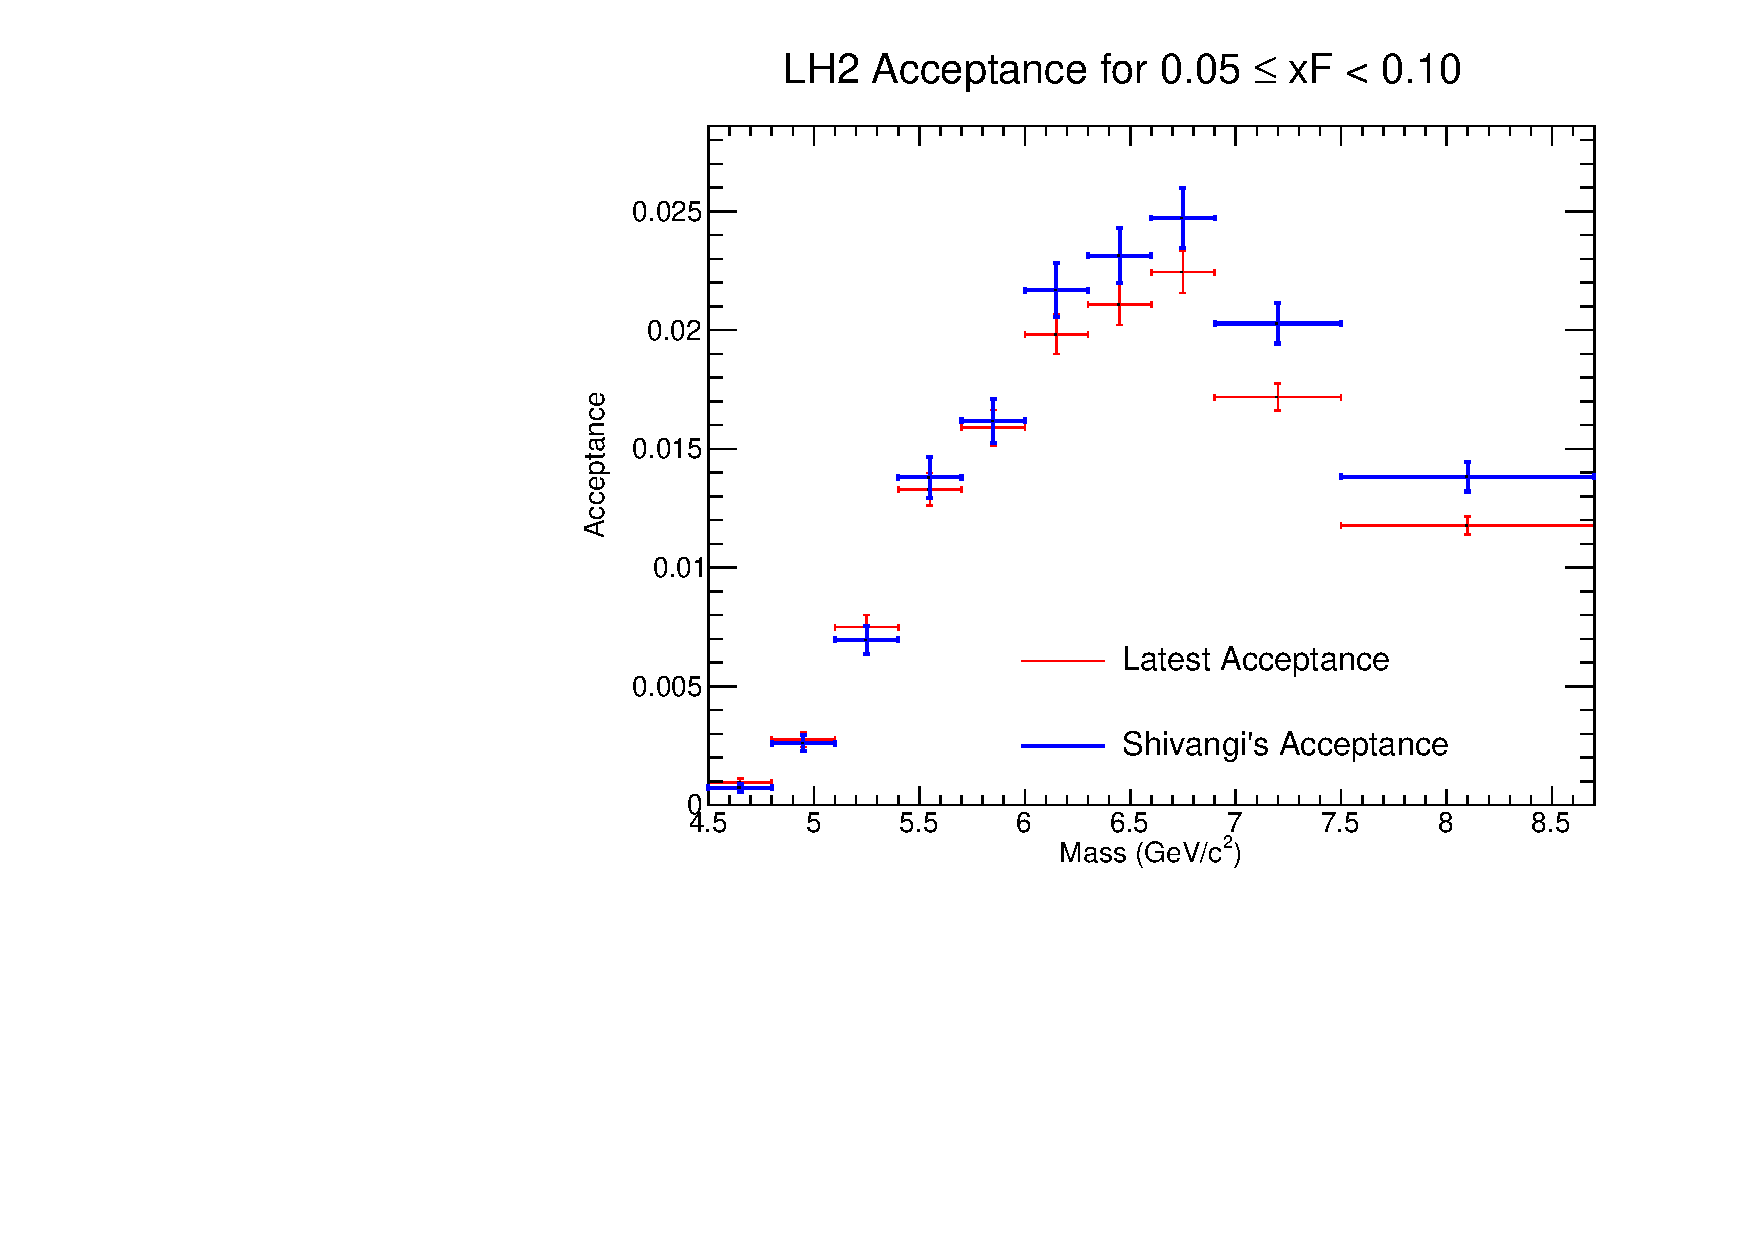
\includegraphics[width=\linewidth]{./acceptancePlots/LH2_acceptance_xF_bin_1.pdf}
       \caption{Acceptance for LH2}
    \end{subfigure}\hfill
    \begin{subfigure}[b]{0.48\textwidth}
       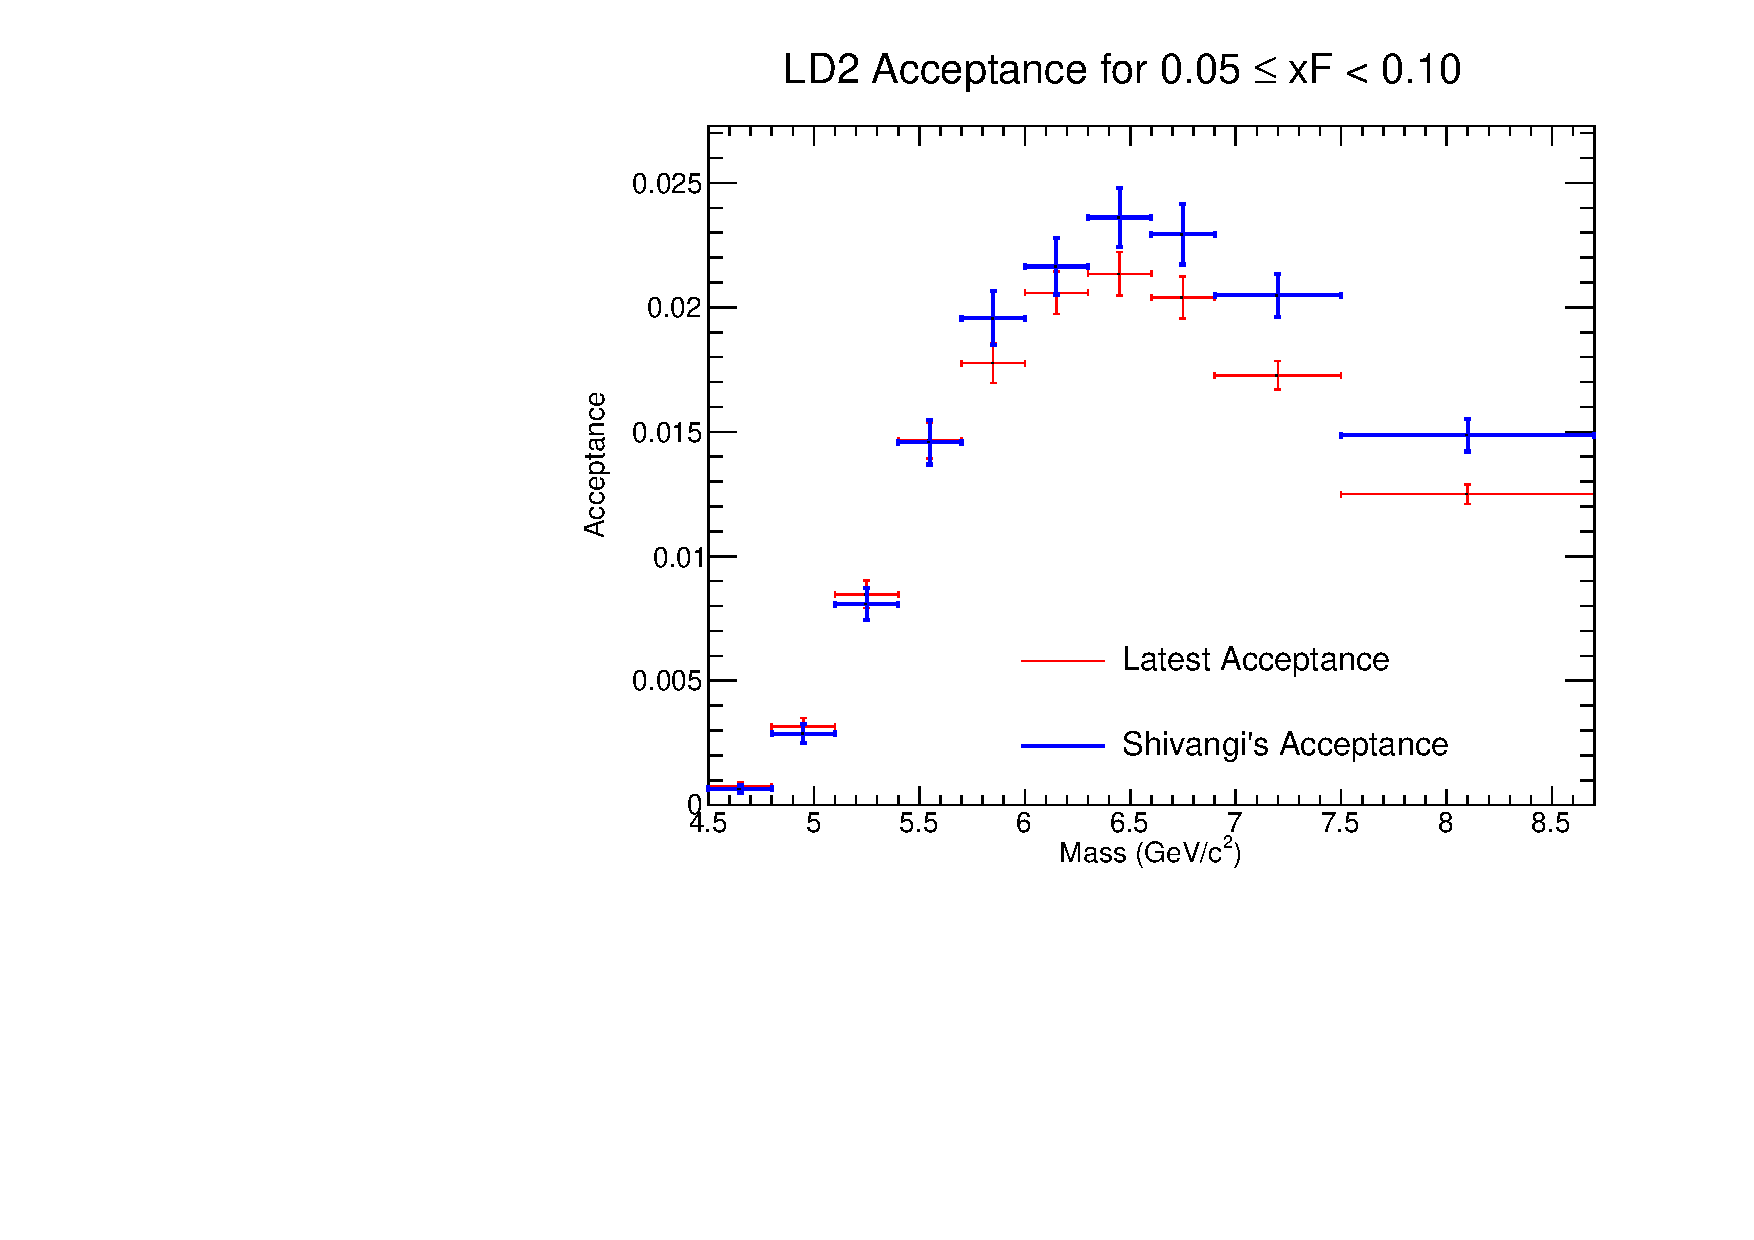
\includegraphics[width=\linewidth]{./acceptancePlots/LD2_acceptance_xF_bin_1.pdf}
       \caption{Acceptance for LD2}
    \end{subfigure}
    \begin{subfigure}[b]{0.48\textwidth}
       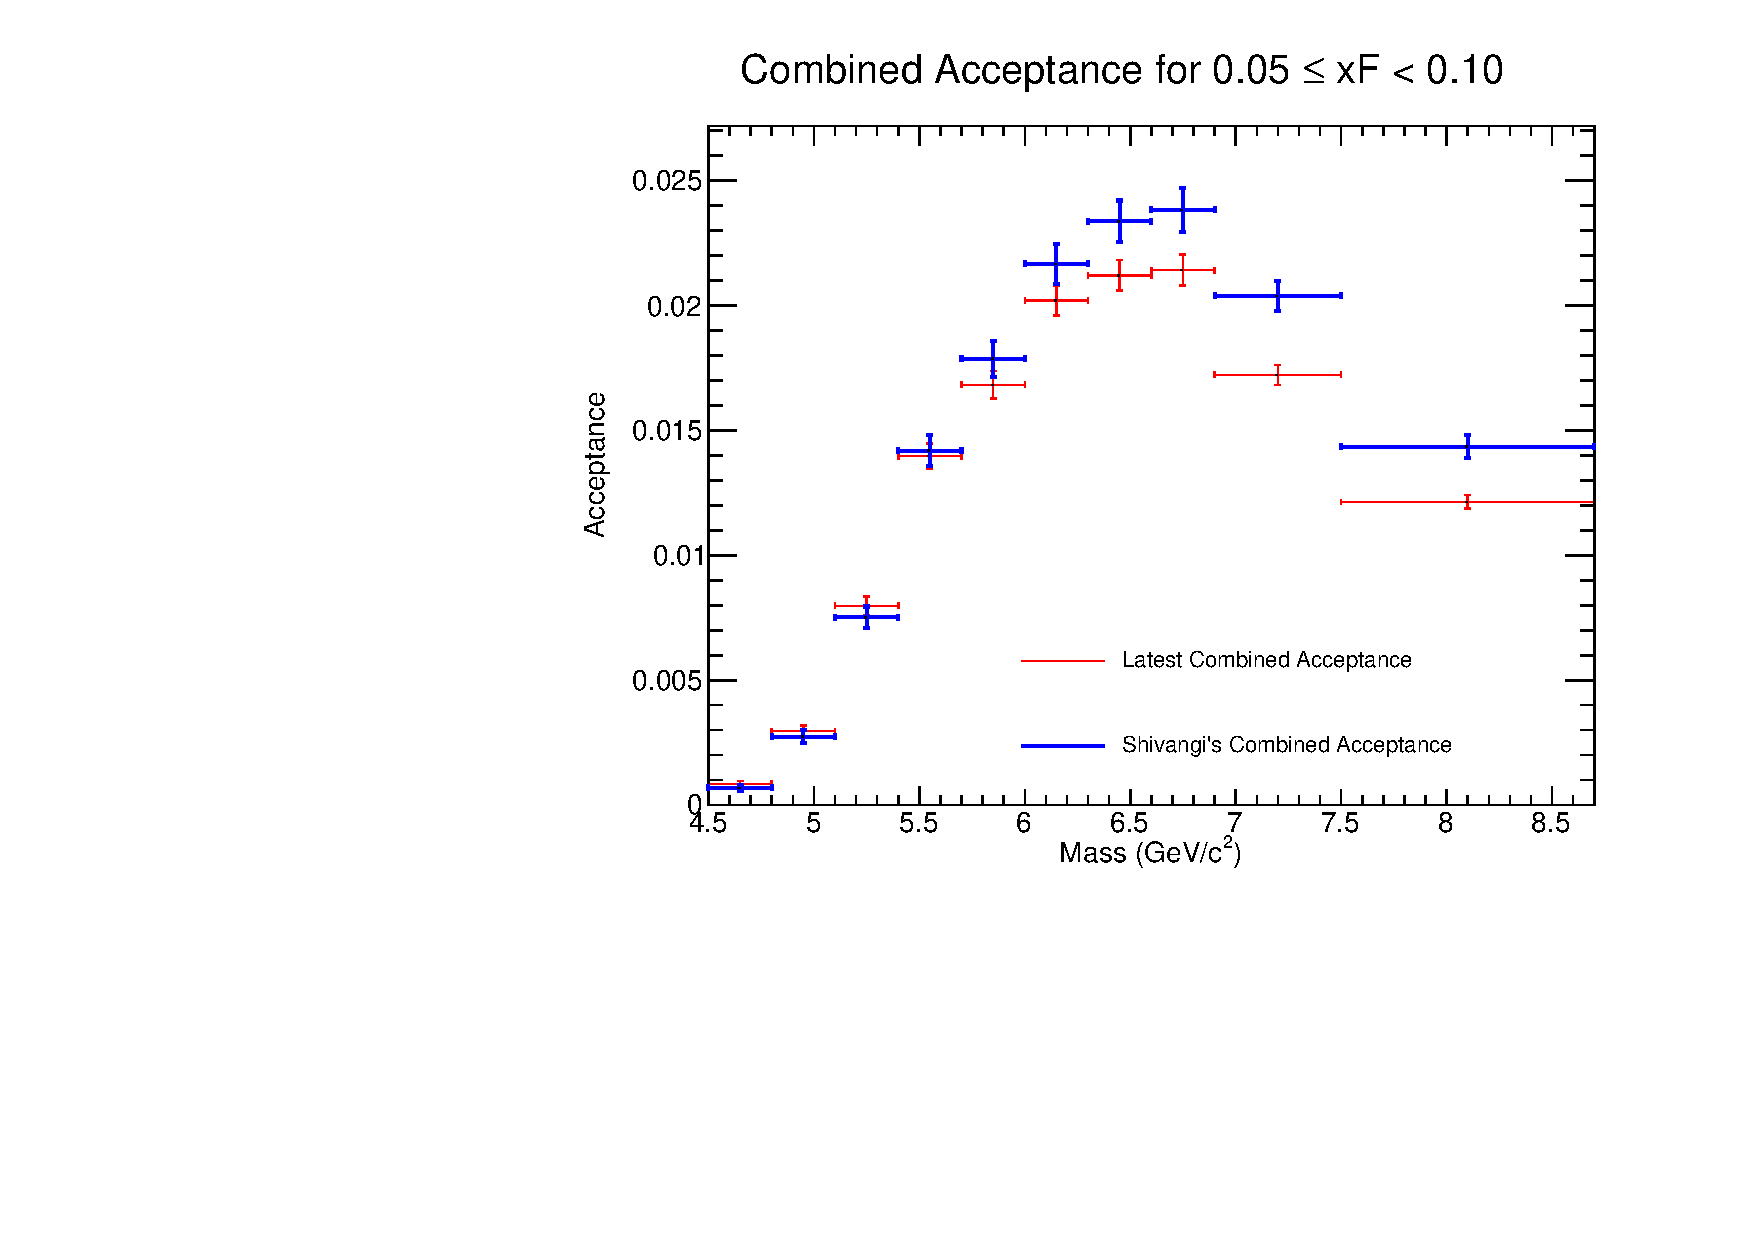
\includegraphics[width=\linewidth]{./acceptancePlots/Combined_acceptance_xF_bin_1.pdf}
       \caption{Combined Acceptance}
    \end{subfigure}\hfill
    \begin{subfigure}[b]{0.48\textwidth}
       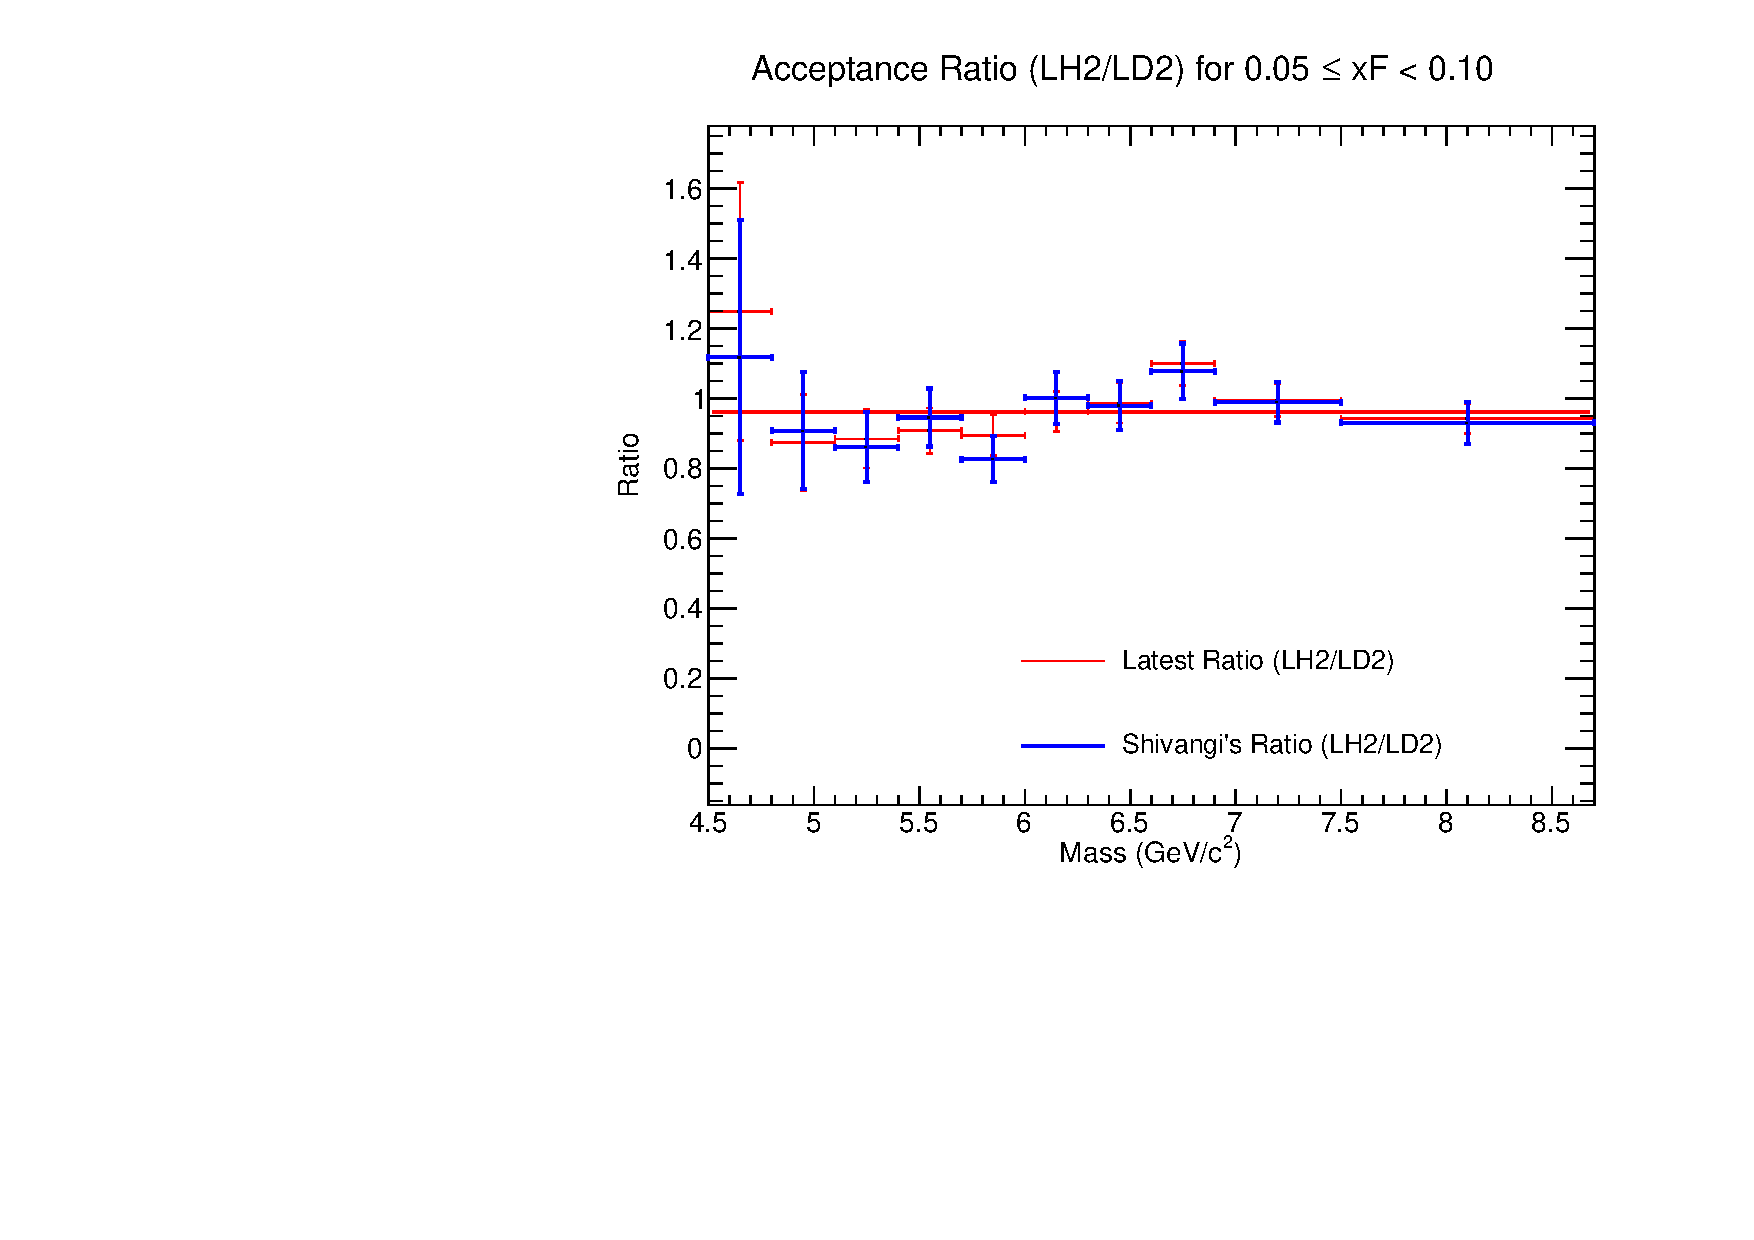
\includegraphics[width=\linewidth]{./acceptancePlots/Acceptance_ratio_xF_bin_1.pdf}
       \caption{Acceptance Ratio (LH2/LD2)}
    \end{subfigure}
    \caption{Acceptance plots for $0.05 \le x_F < 0.10$.}
\end{figure}

\begin{figure}[p]
    \centering
    \begin{subfigure}[b]{0.48\textwidth}
       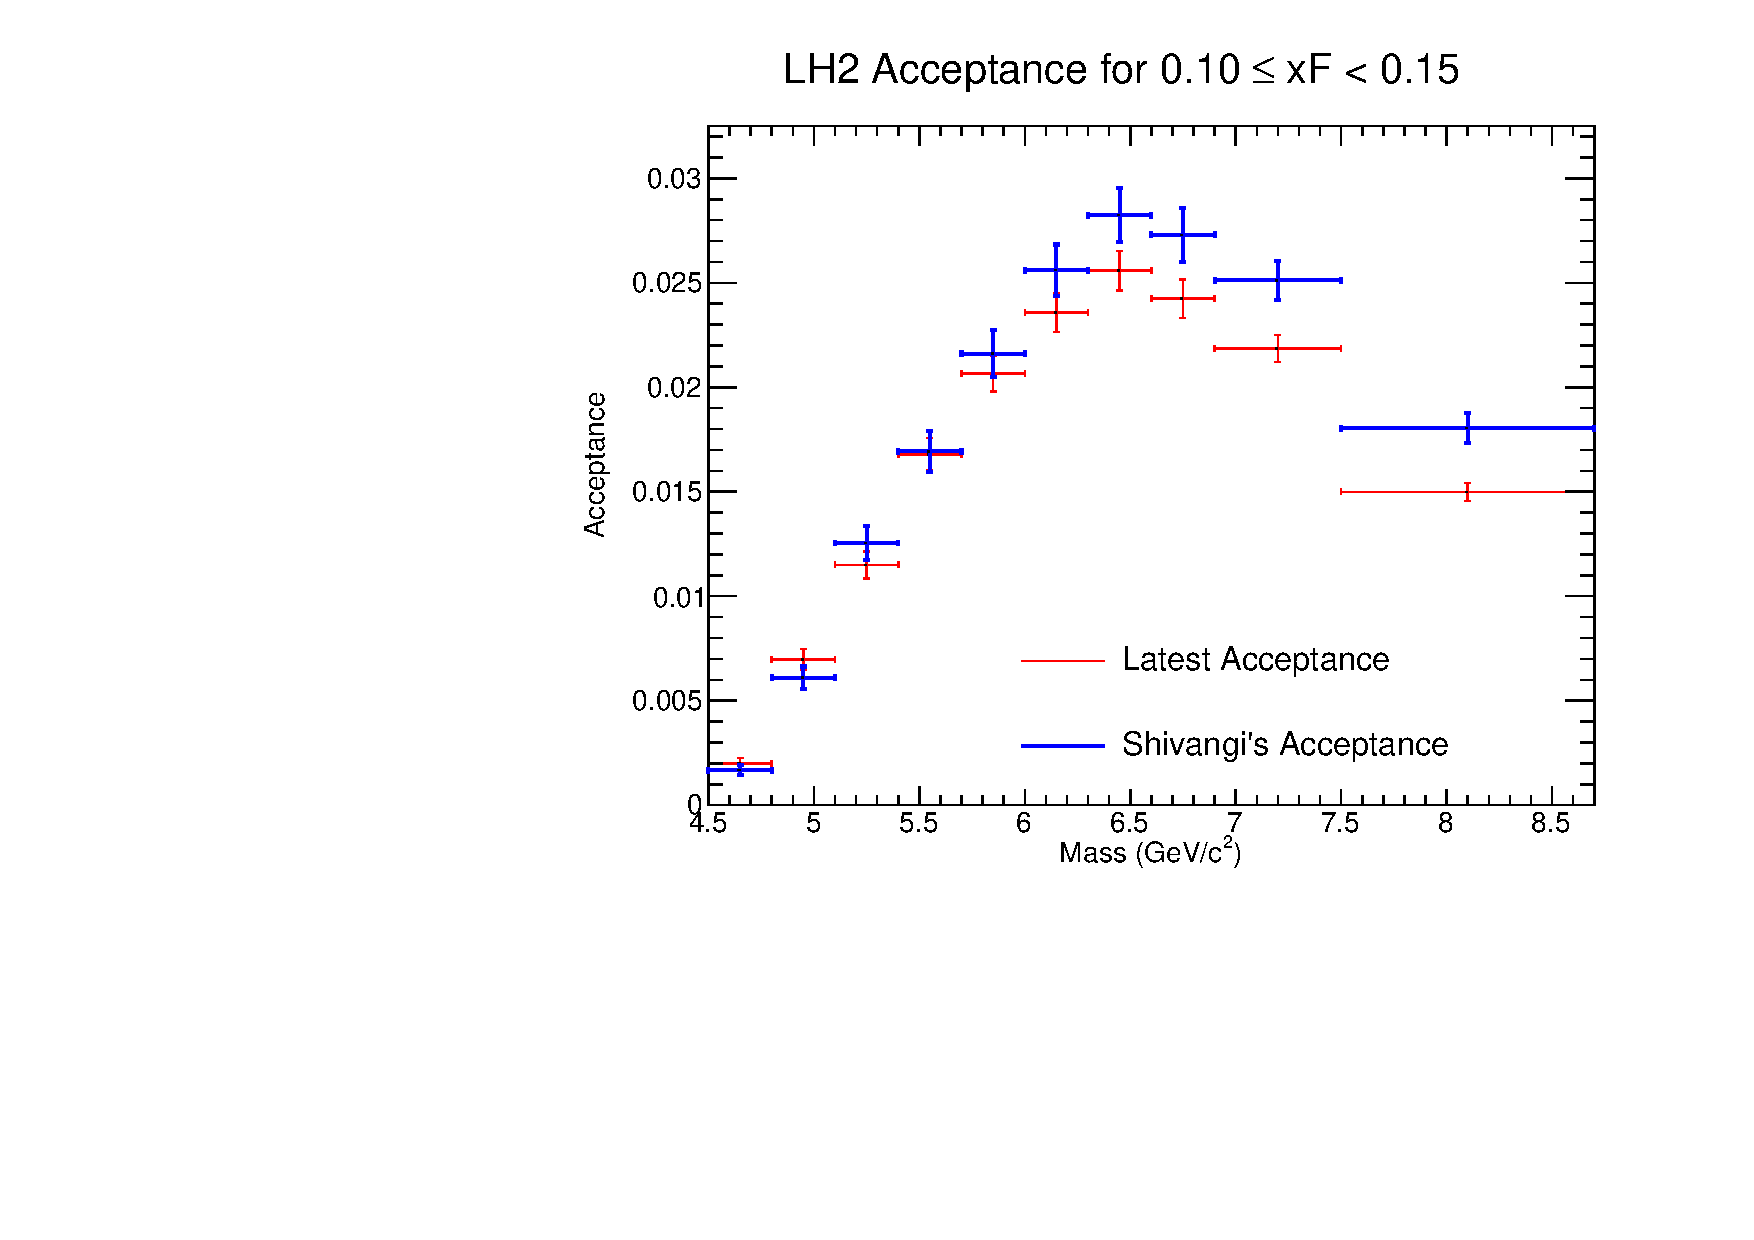
\includegraphics[width=\linewidth]{./acceptancePlots/LH2_acceptance_xF_bin_2.pdf}
       \caption{Acceptance for LH2}
    \end{subfigure}\hfill
    \begin{subfigure}[b]{0.48\textwidth}
       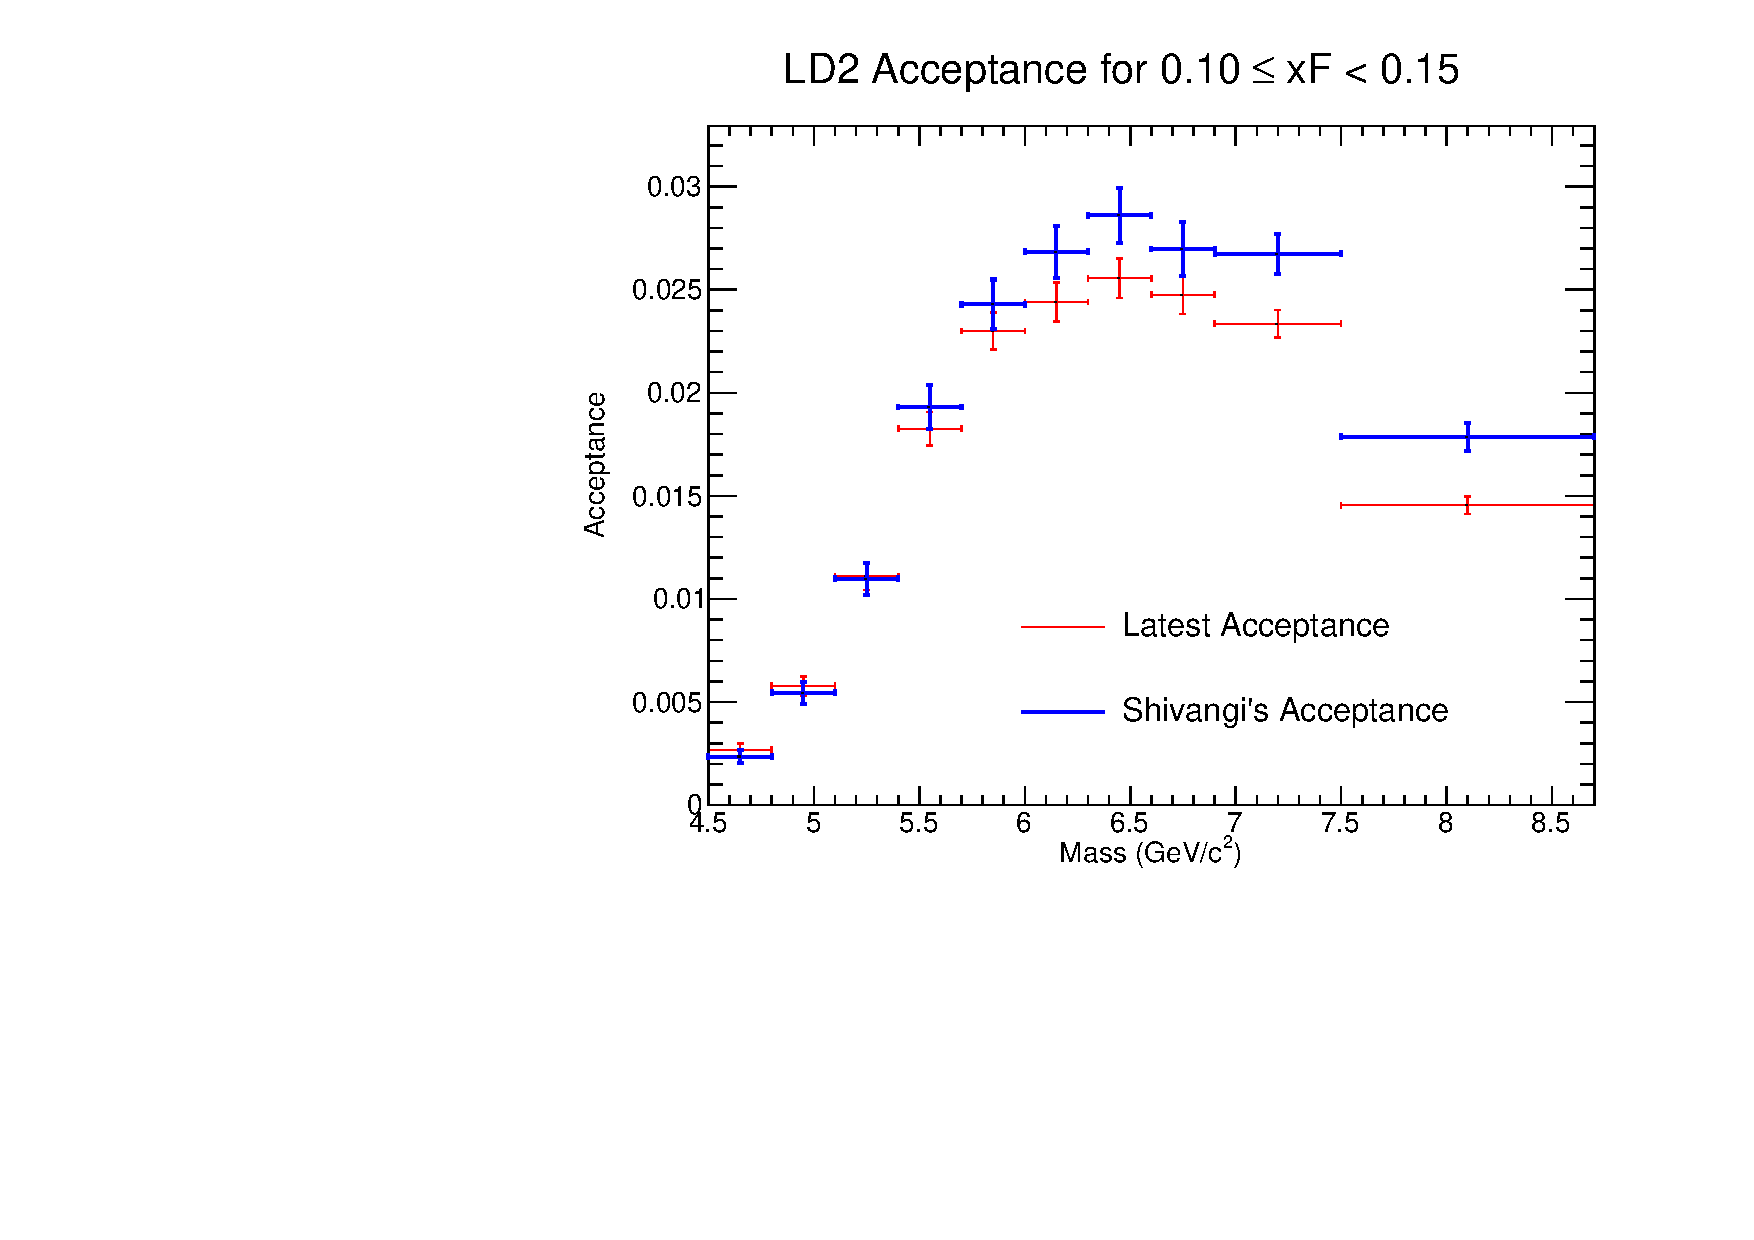
\includegraphics[width=\linewidth]{./acceptancePlots/LD2_acceptance_xF_bin_2.pdf}
       \caption{Acceptance for LD2}
    \end{subfigure}
    \begin{subfigure}[b]{0.48\textwidth}
       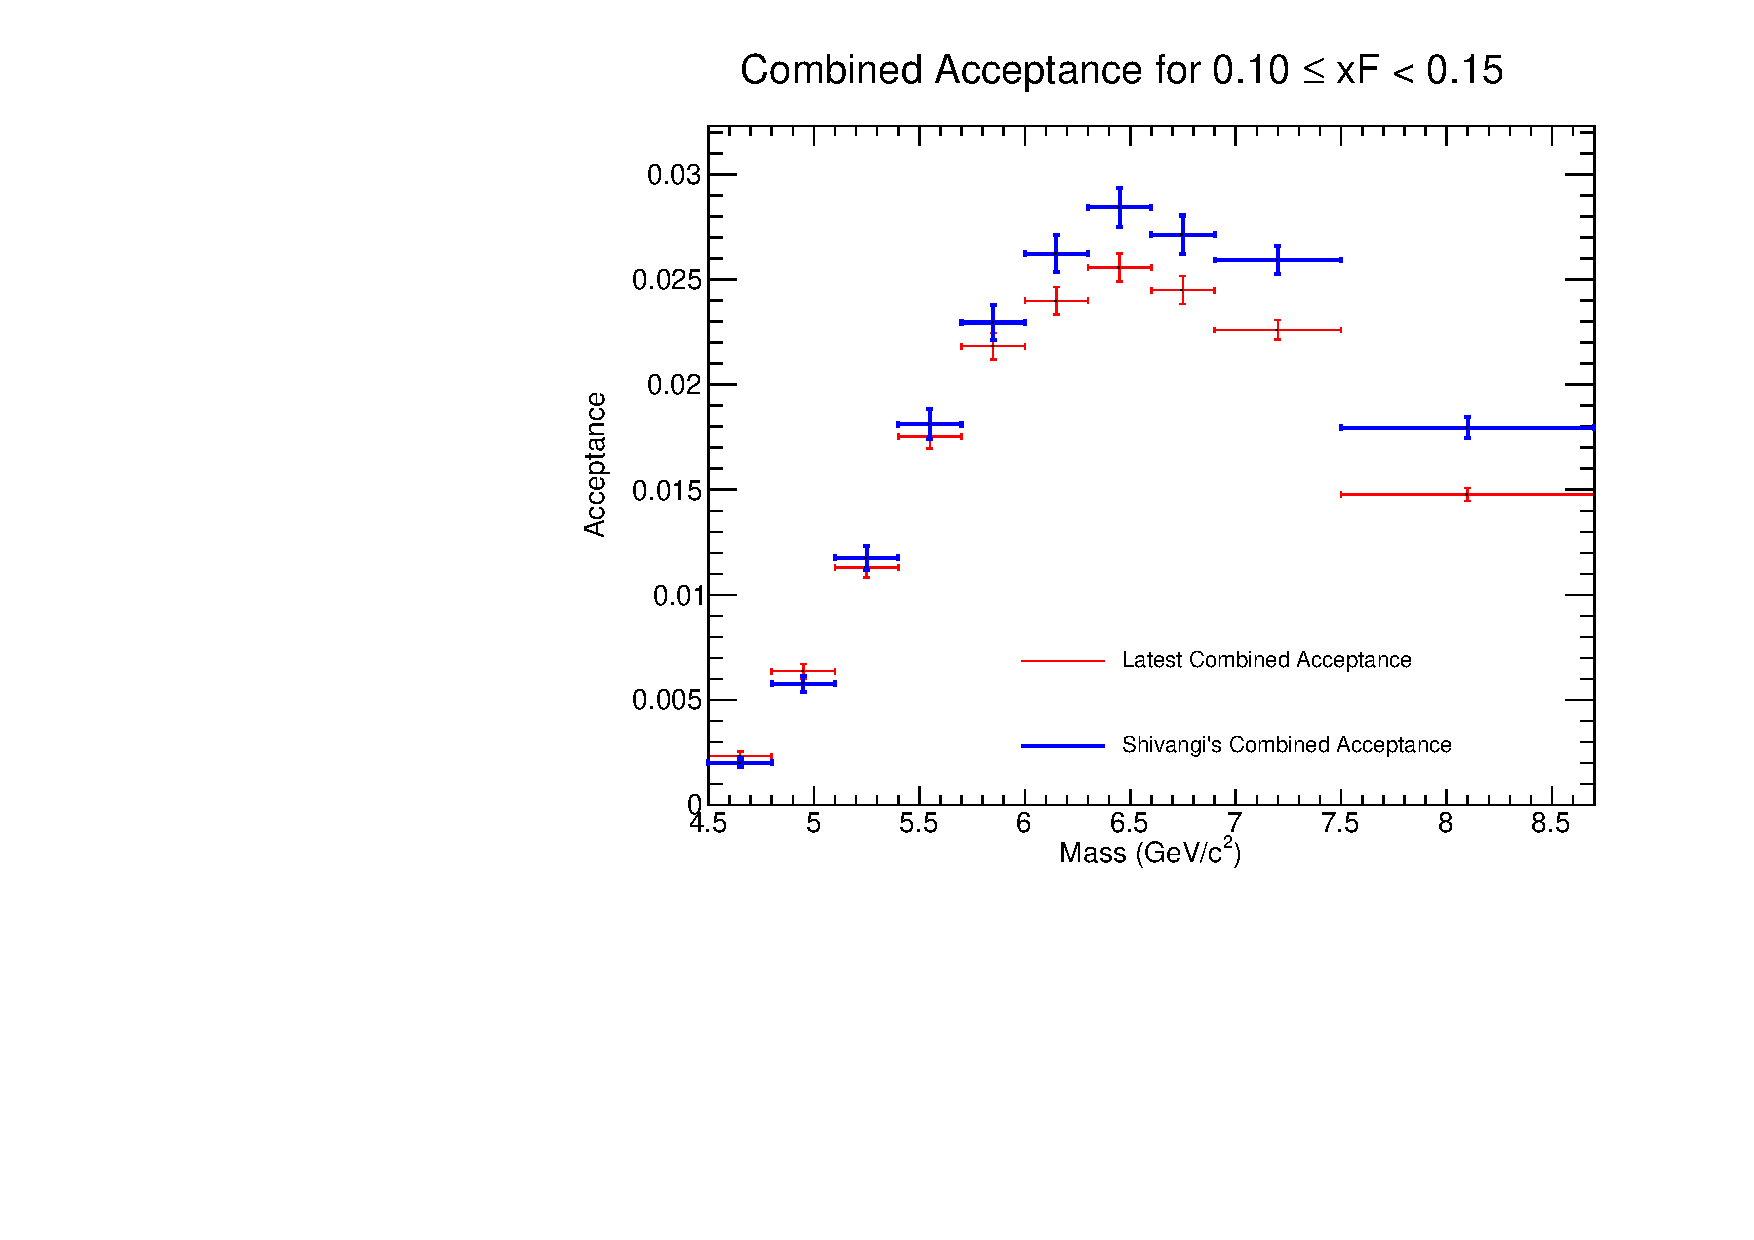
\includegraphics[width=\linewidth]{./acceptancePlots/Combined_acceptance_xF_bin_2.pdf}
       \caption{Combined Acceptance}
    \end{subfigure}\hfill
    \begin{subfigure}[b]{0.48\textwidth}
       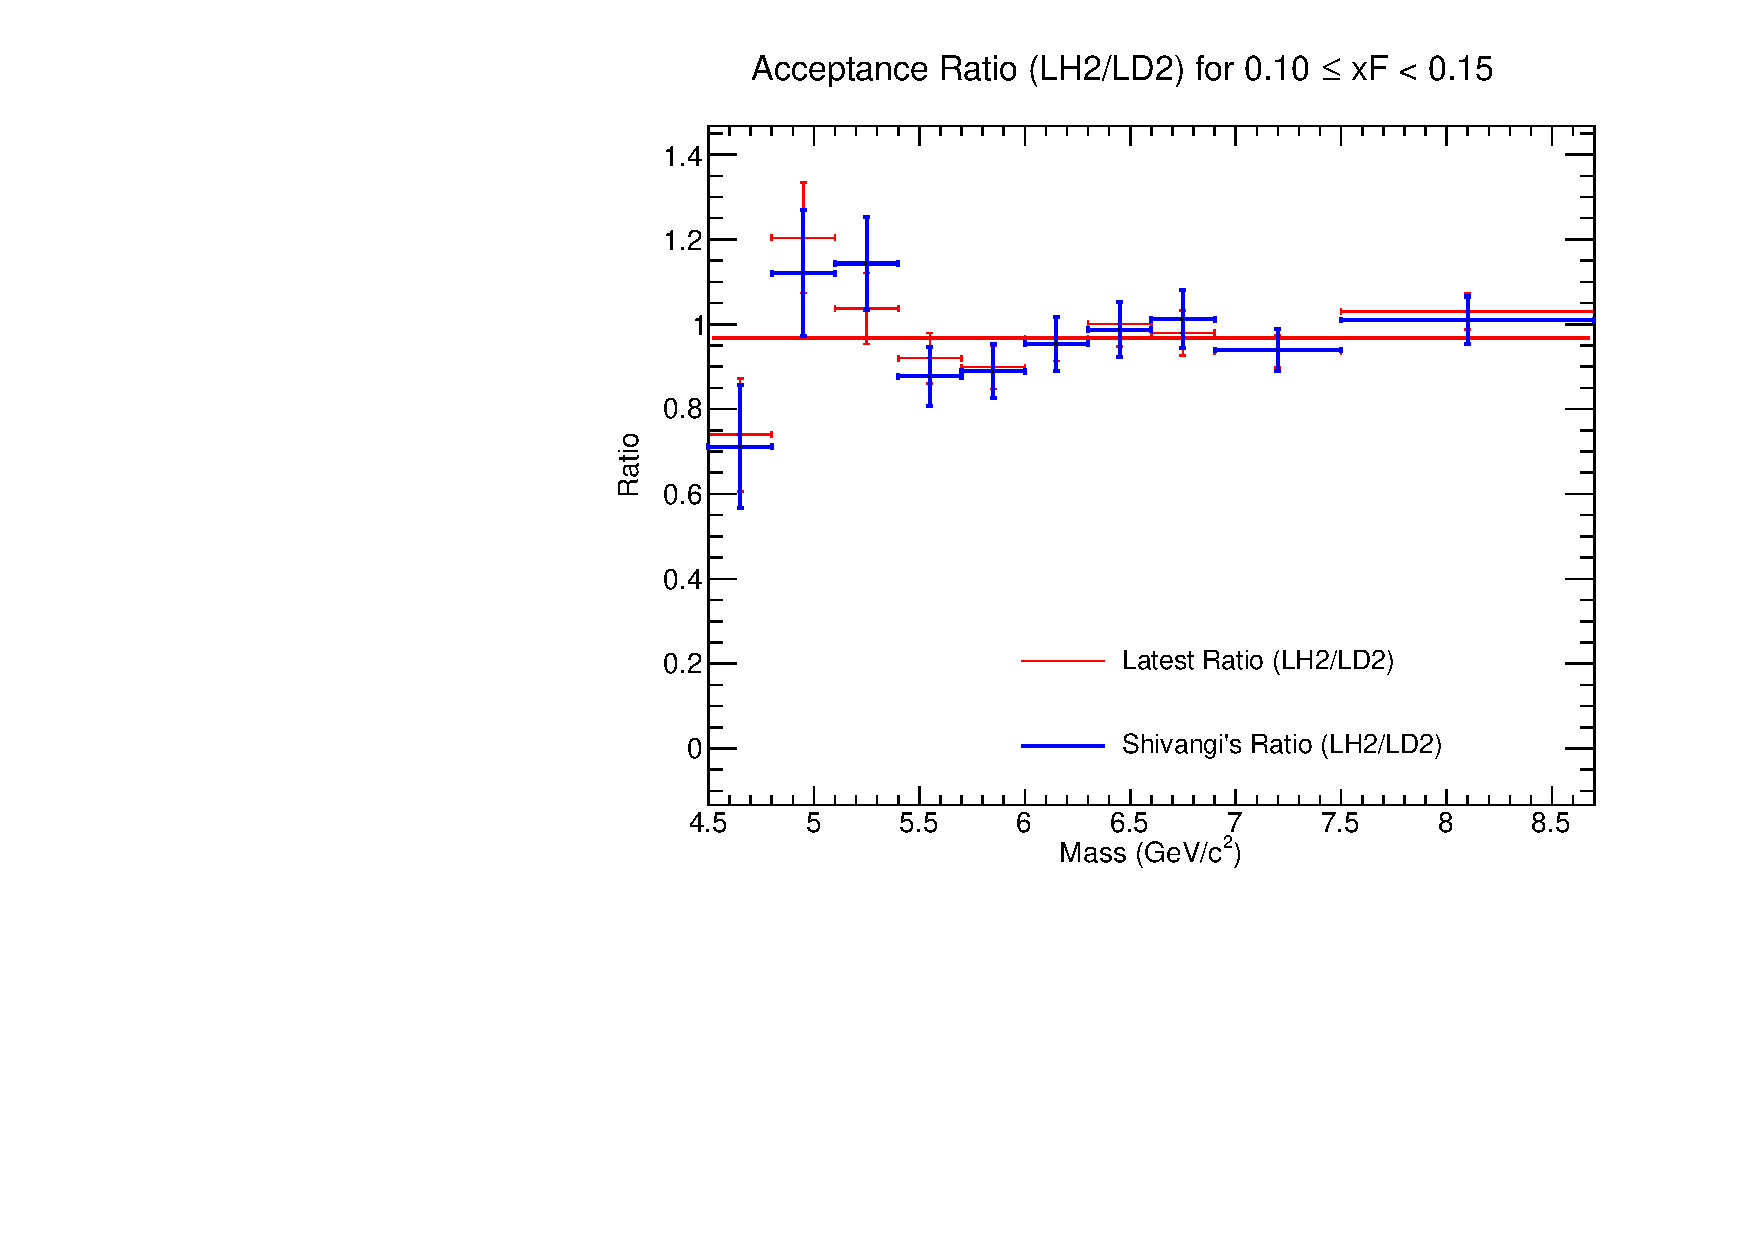
\includegraphics[width=\linewidth]{./acceptancePlots/Acceptance_ratio_xF_bin_2.pdf}
       \caption{Acceptance Ratio (LH2/LD2)}
    \end{subfigure}
    \caption{Acceptance plots for $0.10 \le x_F < 0.15$.}
\end{figure}

\begin{figure}[p]
    \centering
    \begin{subfigure}[b]{0.48\textwidth}
       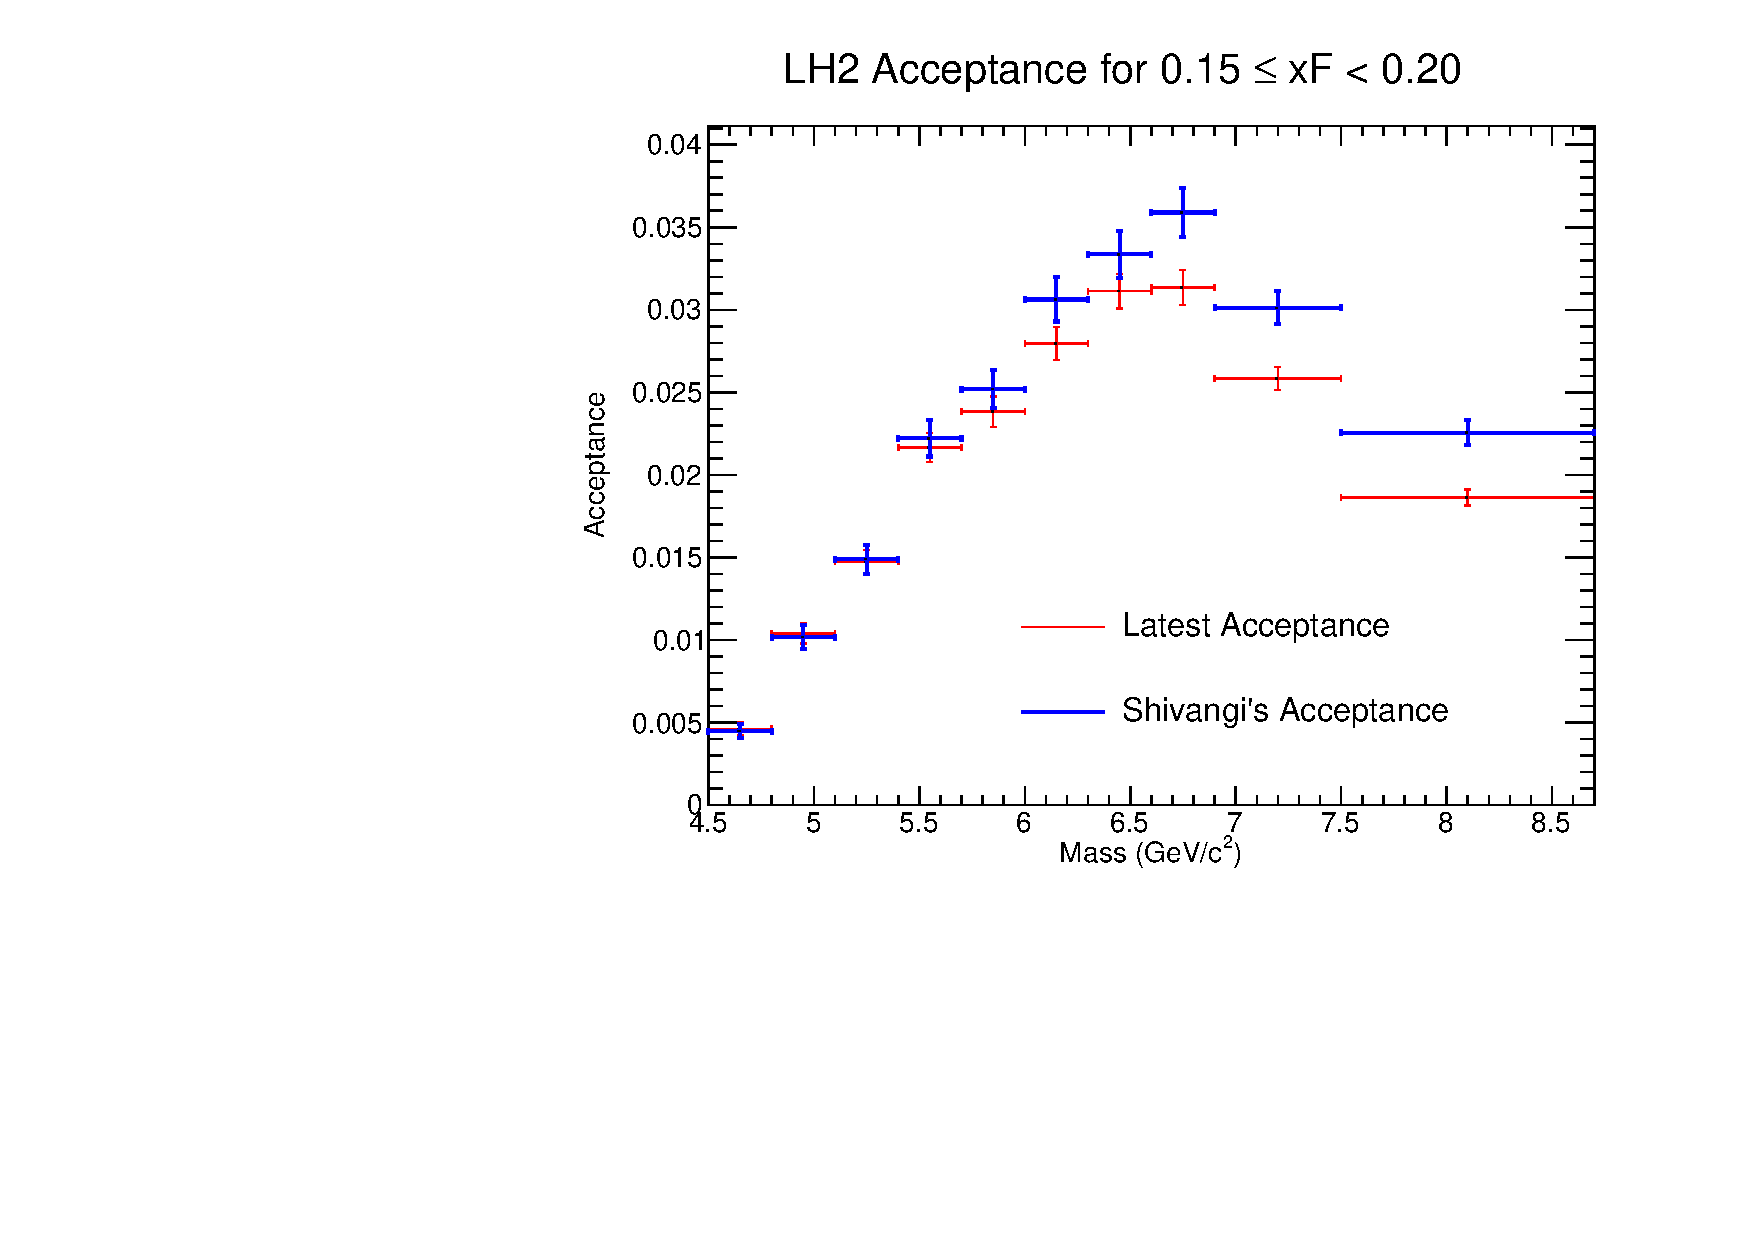
\includegraphics[width=\linewidth]{./acceptancePlots/LH2_acceptance_xF_bin_3.pdf}
       \caption{Acceptance for LH2}
    \end{subfigure}\hfill
    \begin{subfigure}[b]{0.48\textwidth}
       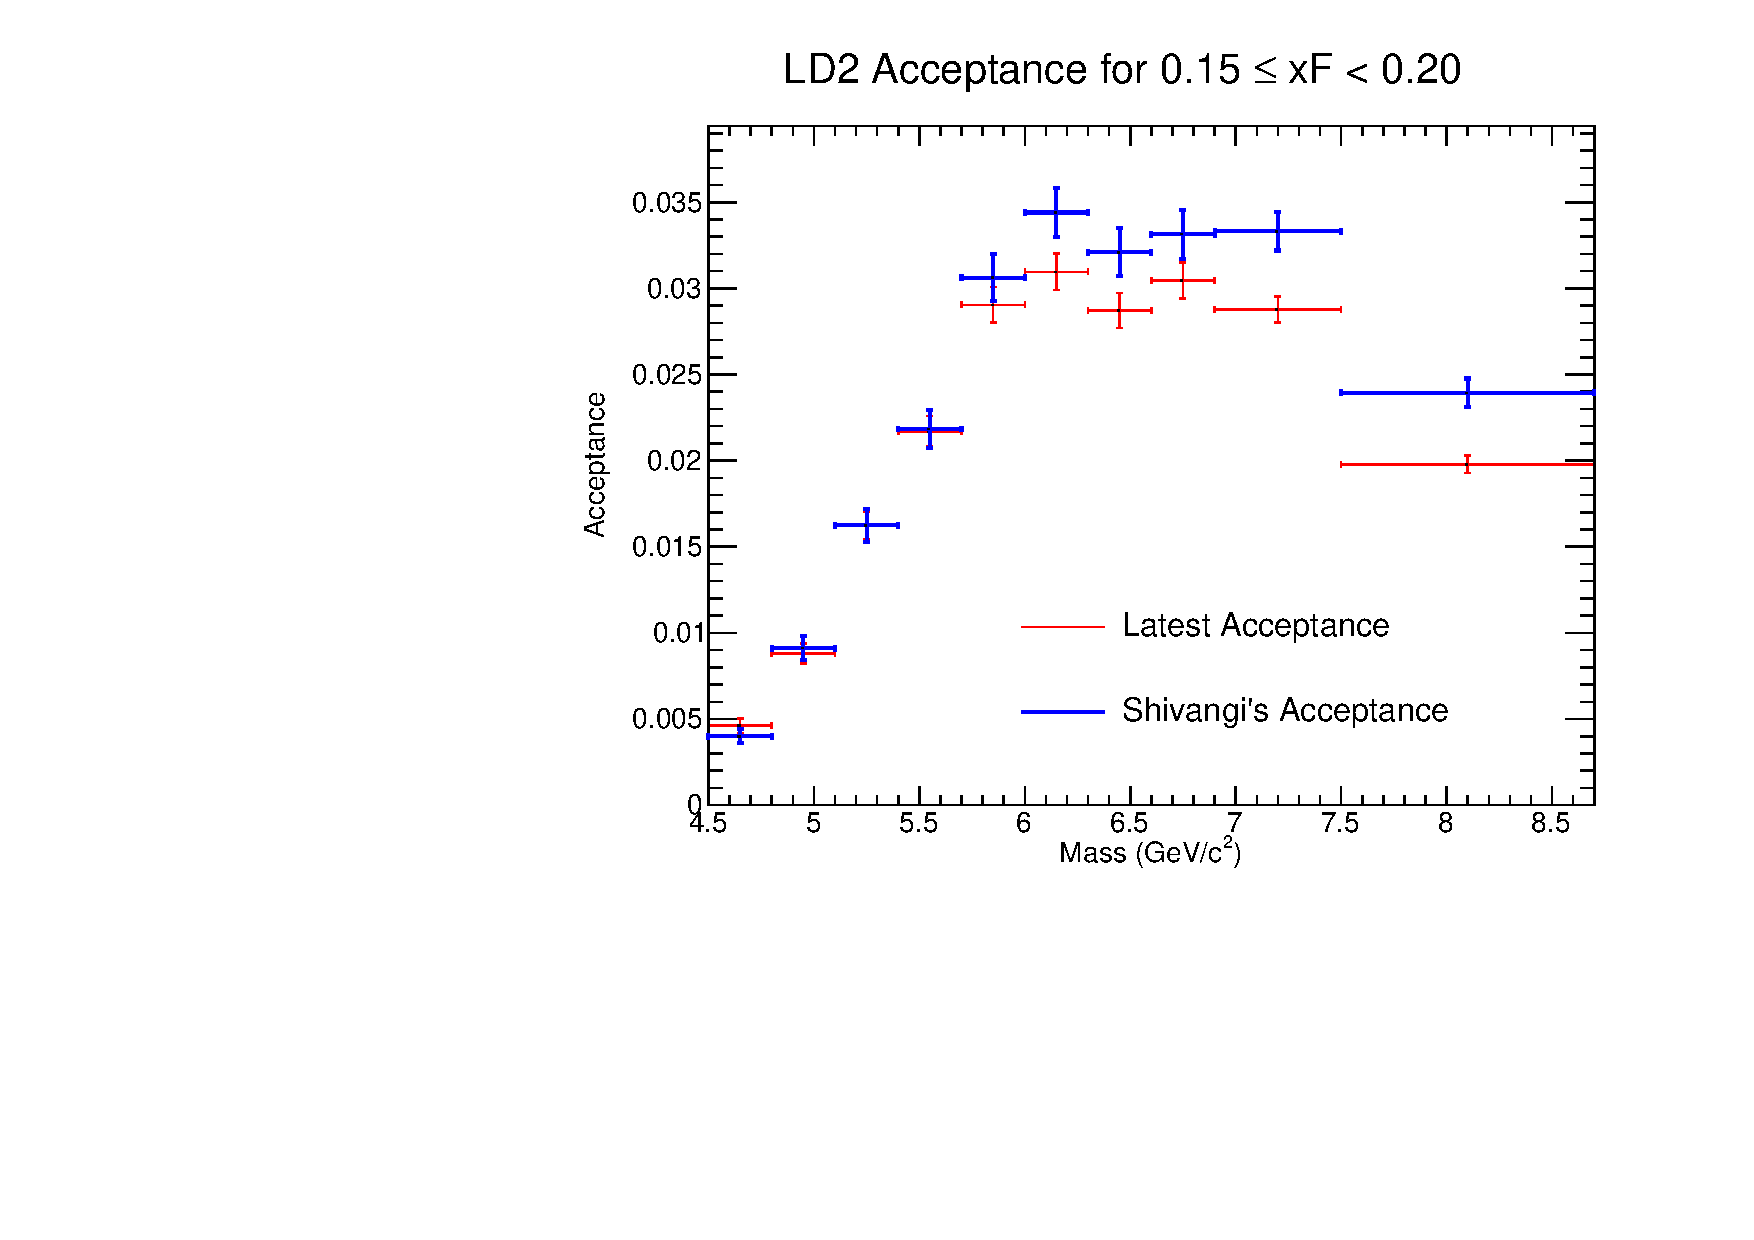
\includegraphics[width=\linewidth]{./acceptancePlots/LD2_acceptance_xF_bin_3.pdf}
       \caption{Acceptance for LD2}
    \end{subfigure}
    \begin{subfigure}[b]{0.48\textwidth}
       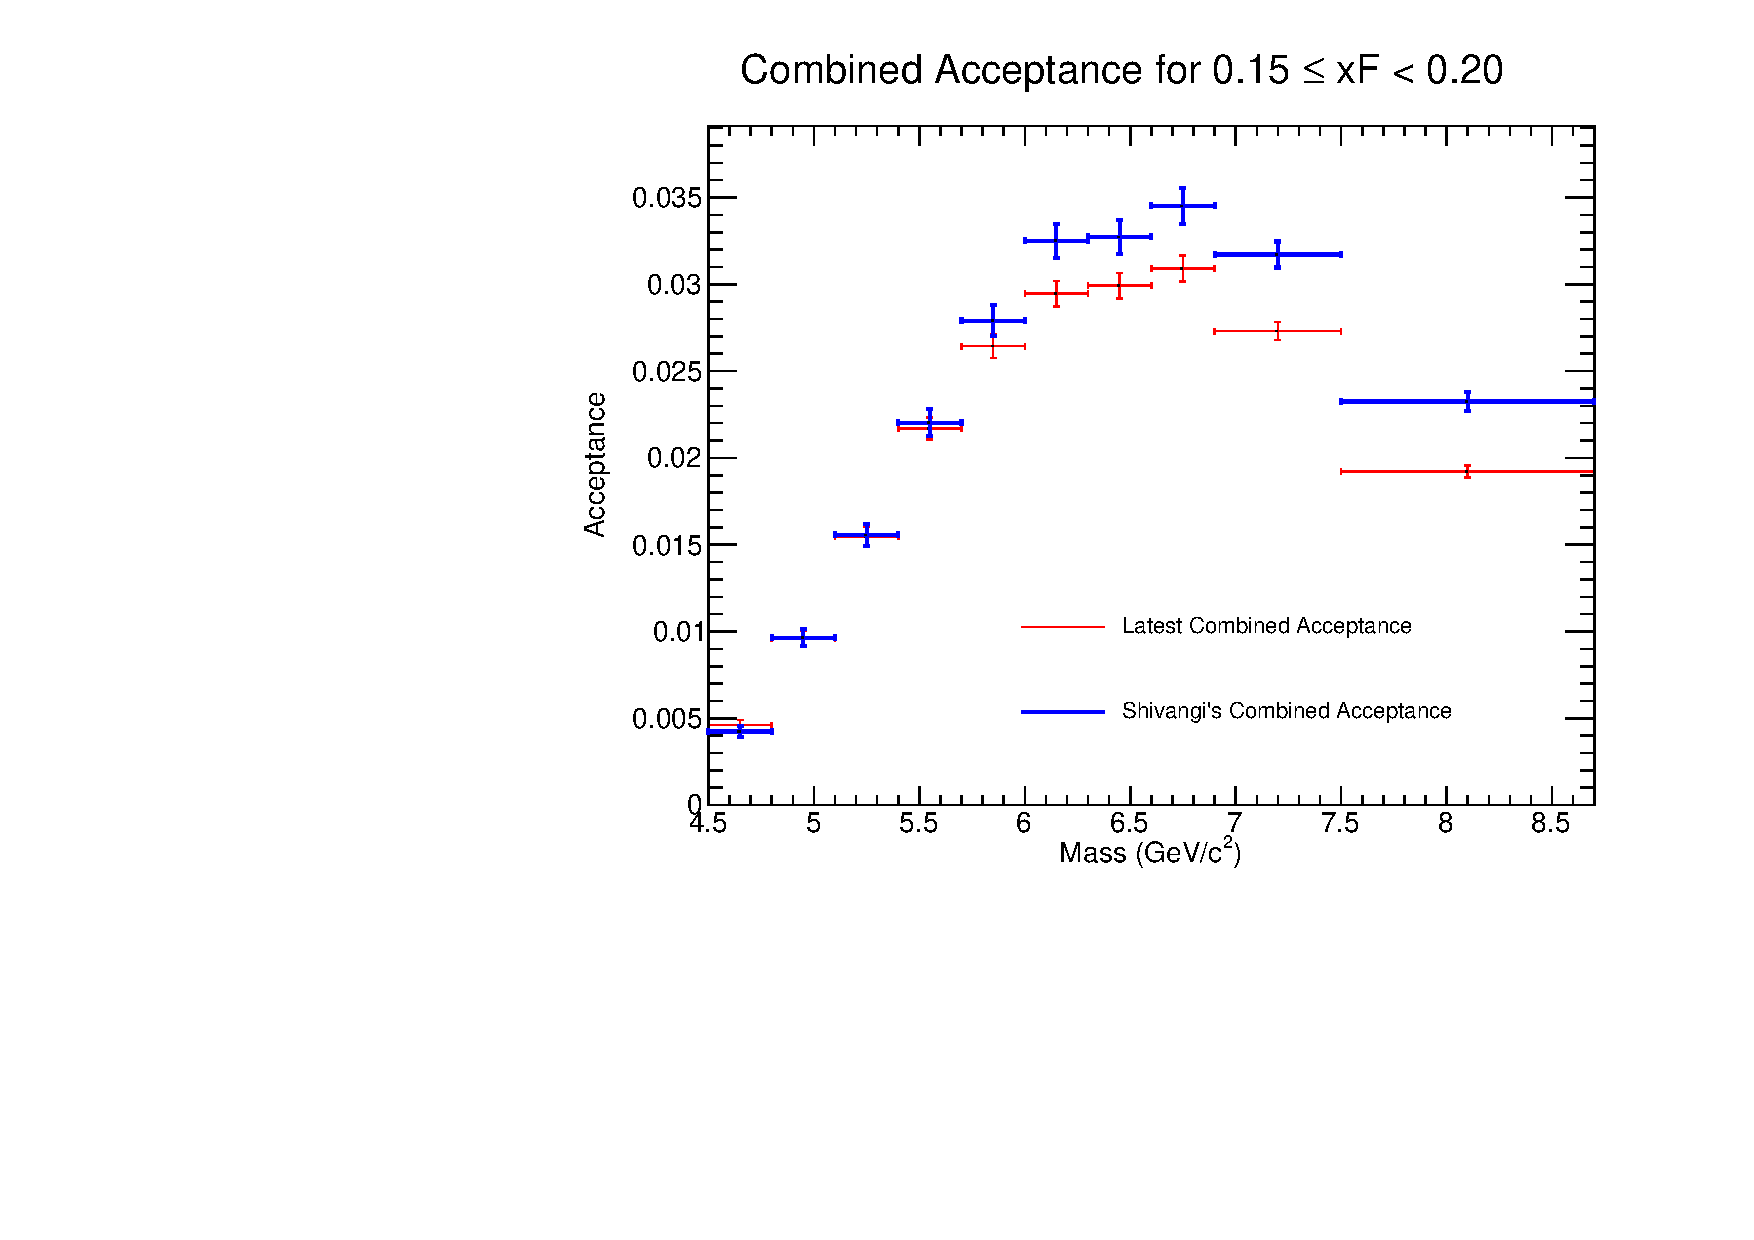
\includegraphics[width=\linewidth]{./acceptancePlots/Combined_acceptance_xF_bin_3.pdf}
       \caption{Combined Acceptance}
    \end{subfigure}\hfill
    \begin{subfigure}[b]{0.48\textwidth}
       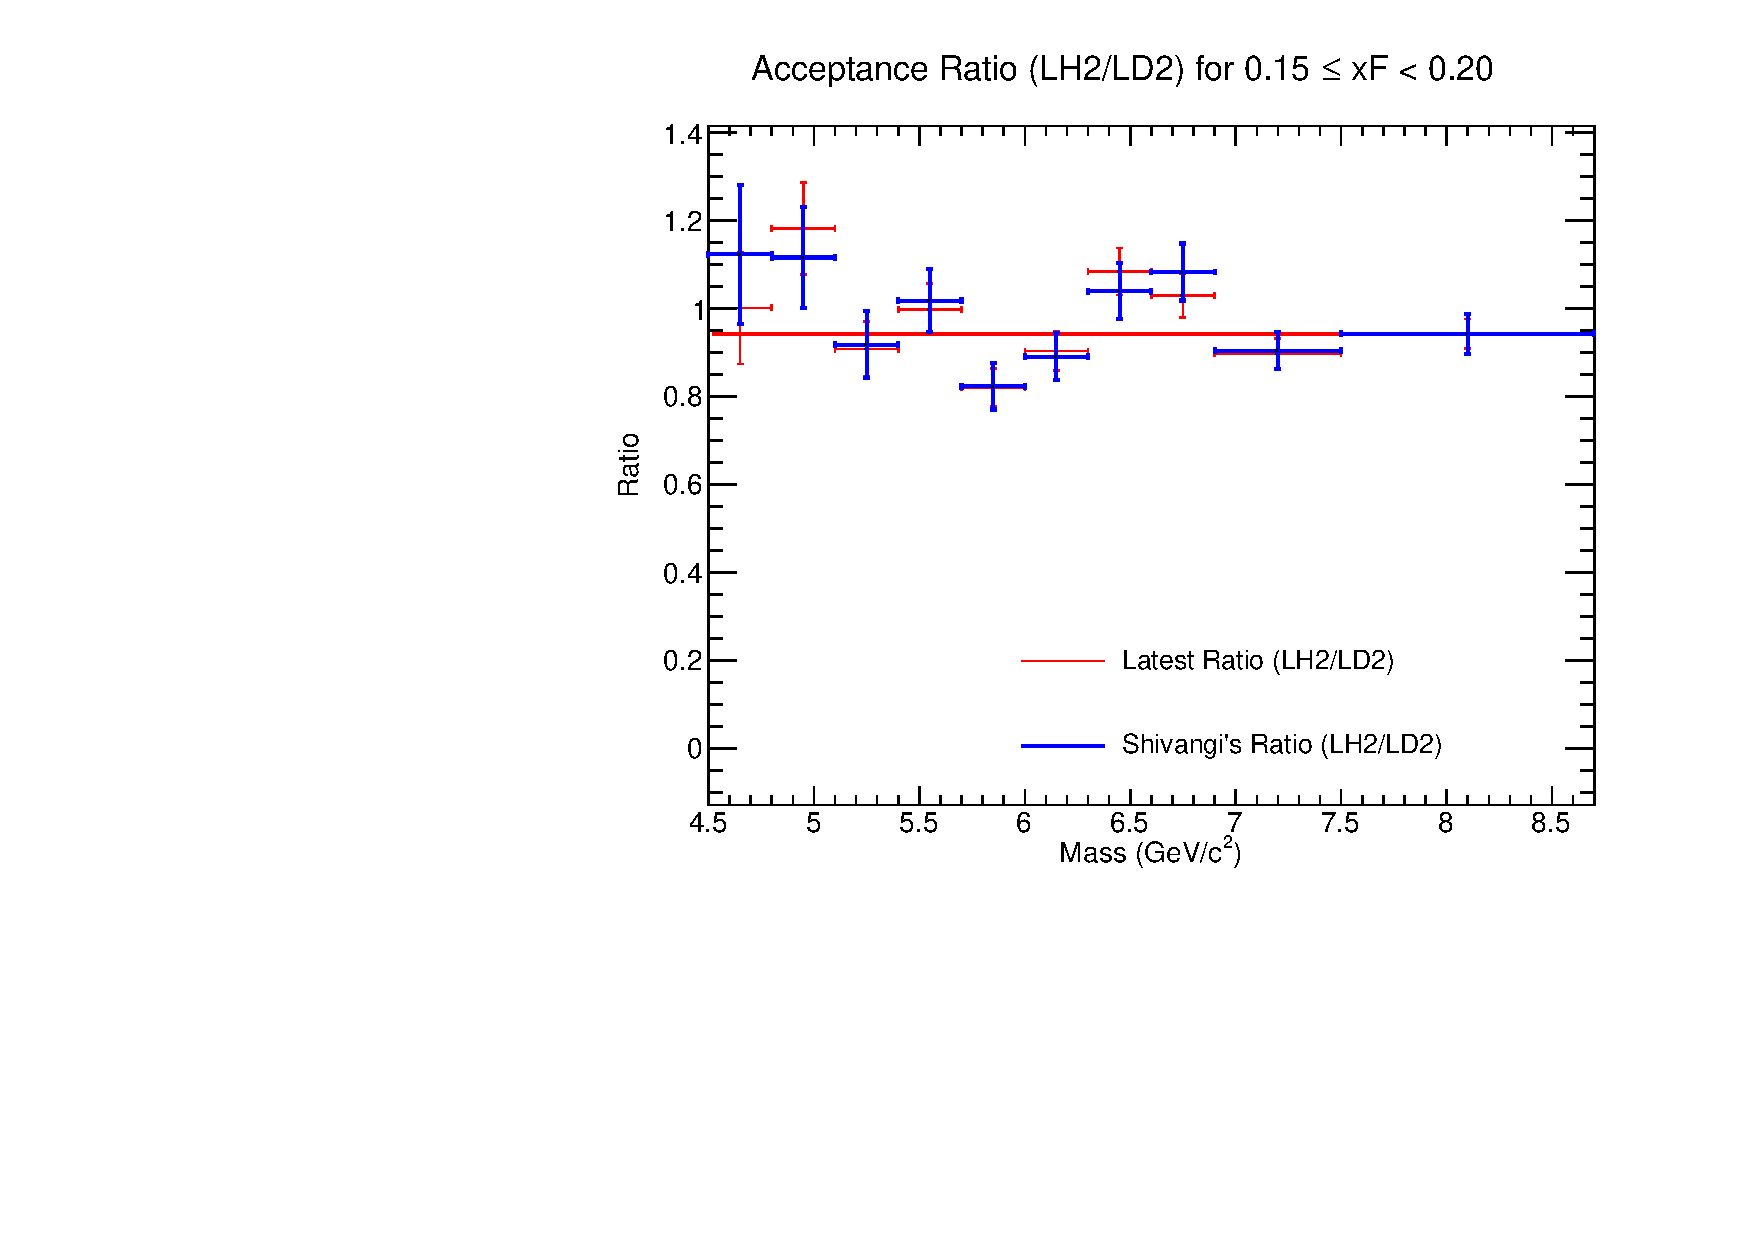
\includegraphics[width=\linewidth]{./acceptancePlots/Acceptance_ratio_xF_bin_3.pdf}
       \caption{Acceptance Ratio (LH2/LD2)}
    \end{subfigure}
    \caption{Acceptance plots for $0.15 \le x_F < 0.20$.}
\end{figure}

\begin{figure}[p]
    \centering
    \begin{subfigure}[b]{0.48\textwidth}
       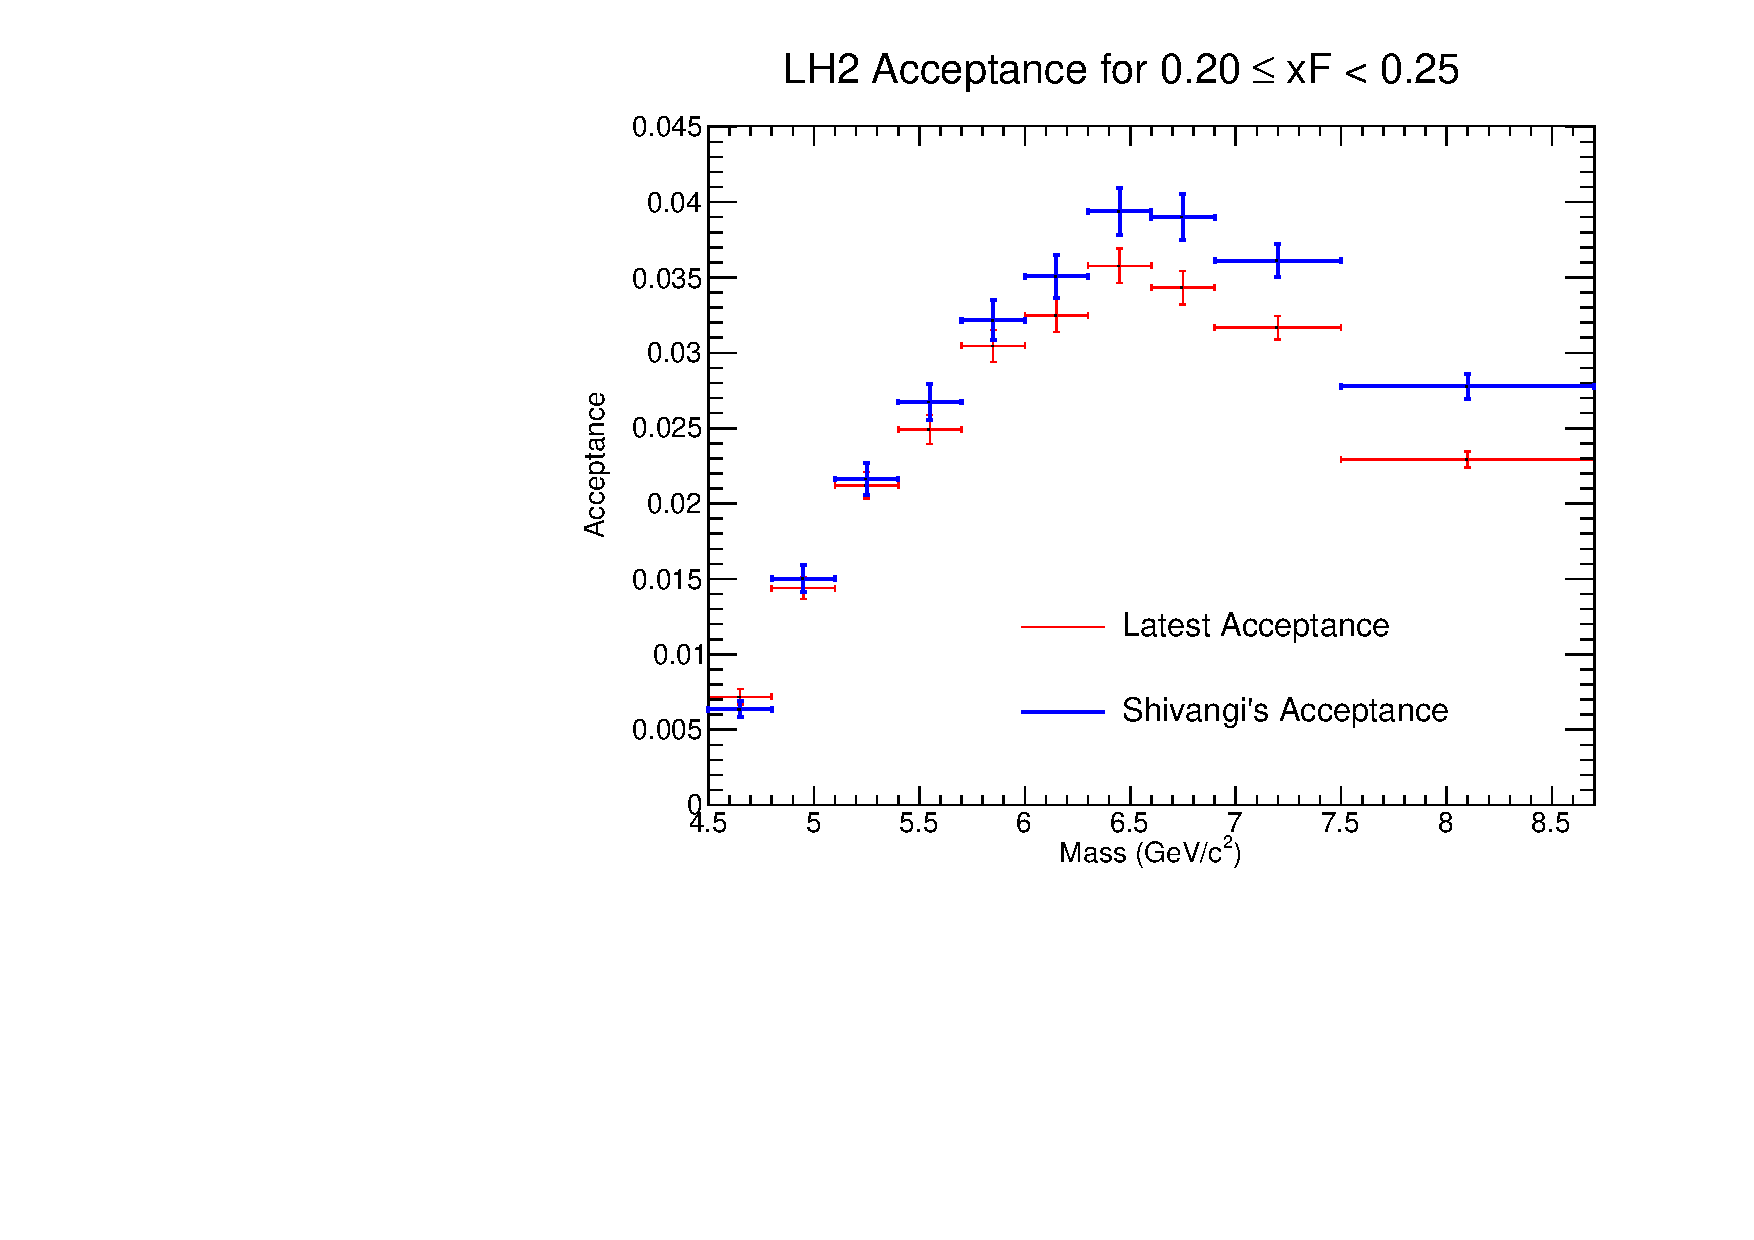
\includegraphics[width=\linewidth]{./acceptancePlots/LH2_acceptance_xF_bin_4.pdf}
       \caption{Acceptance for LH2}
    \end{subfigure}\hfill
    \begin{subfigure}[b]{0.48\textwidth}
       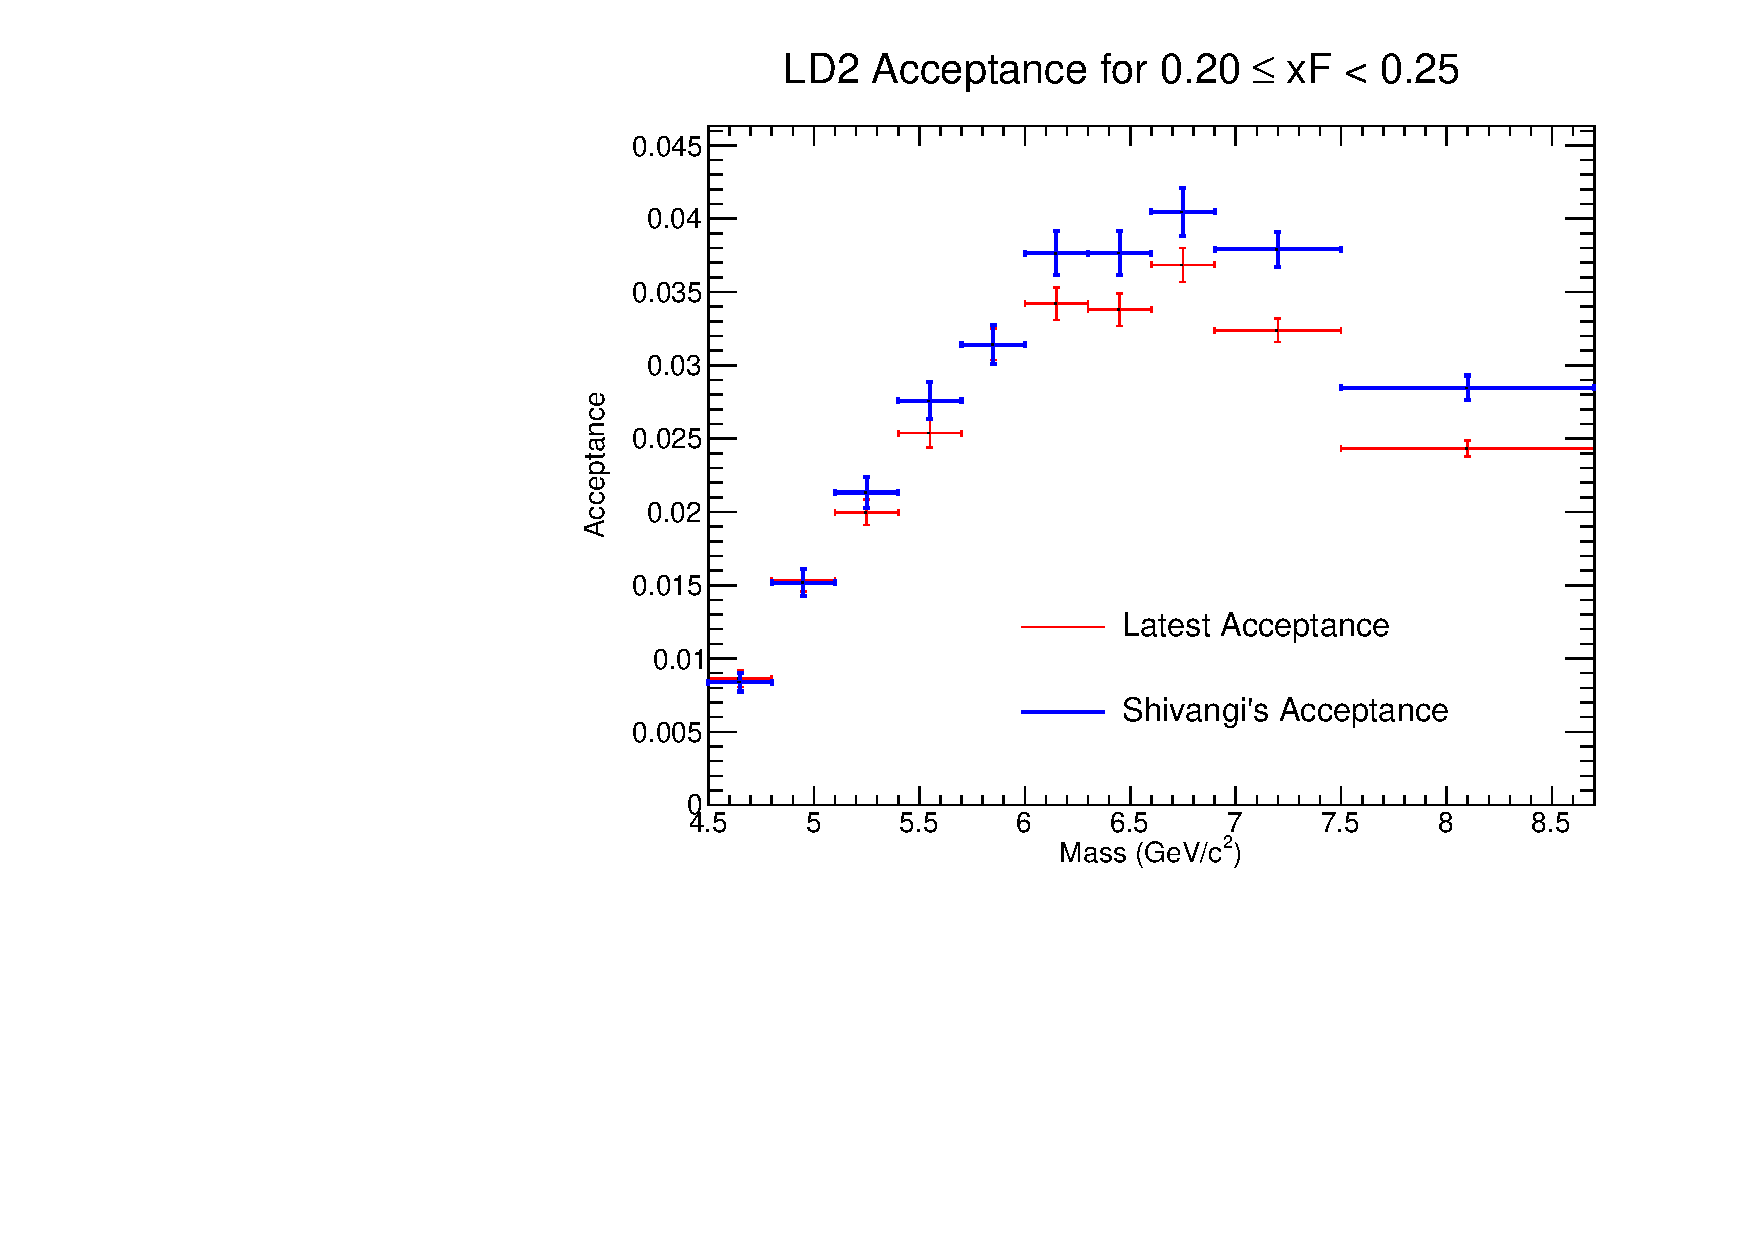
\includegraphics[width=\linewidth]{./acceptancePlots/LD2_acceptance_xF_bin_4.pdf}
       \caption{Acceptance for LD2}
    \end{subfigure}
    \begin{subfigure}[b]{0.48\textwidth}
       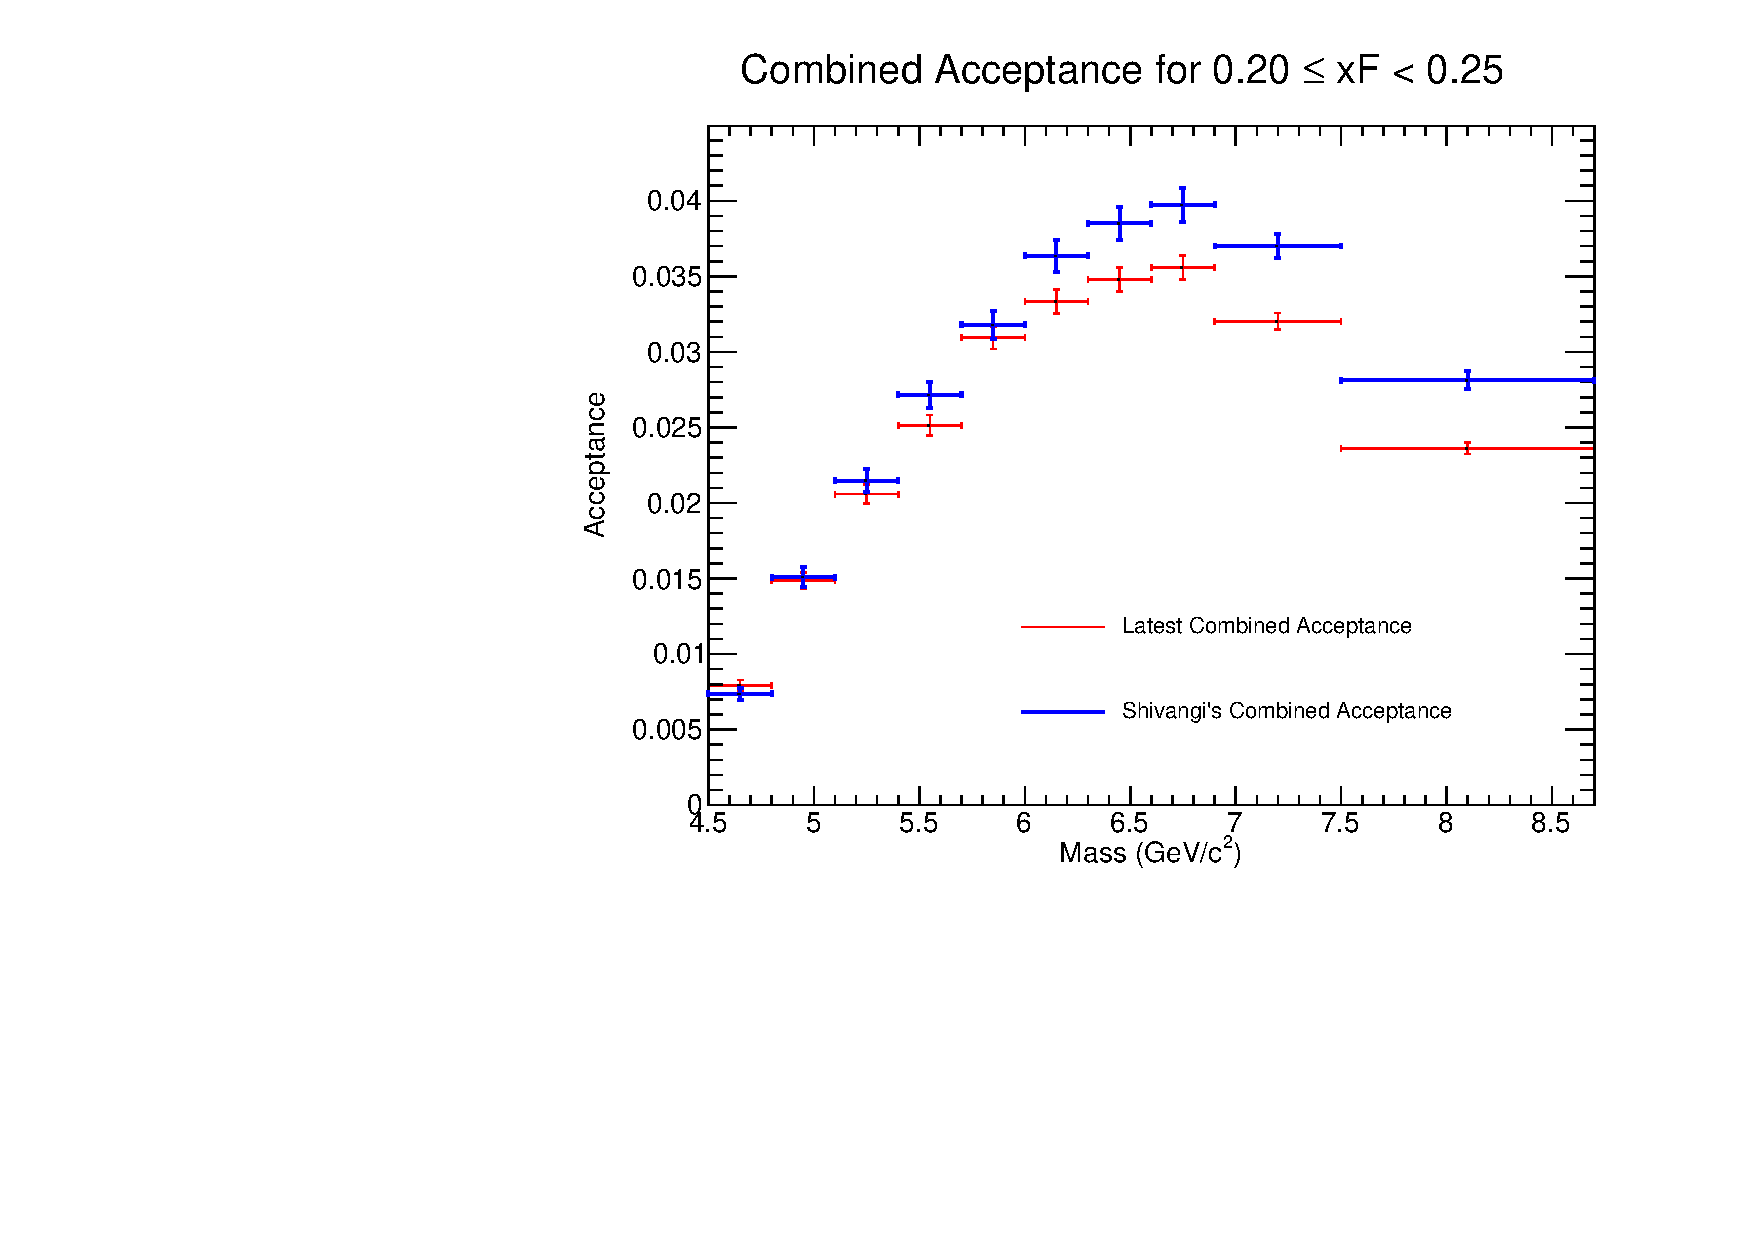
\includegraphics[width=\linewidth]{./acceptancePlots/Combined_acceptance_xF_bin_4.pdf}
       \caption{Combined Acceptance}
    \end{subfigure}\hfill
    \begin{subfigure}[b]{0.48\textwidth}
       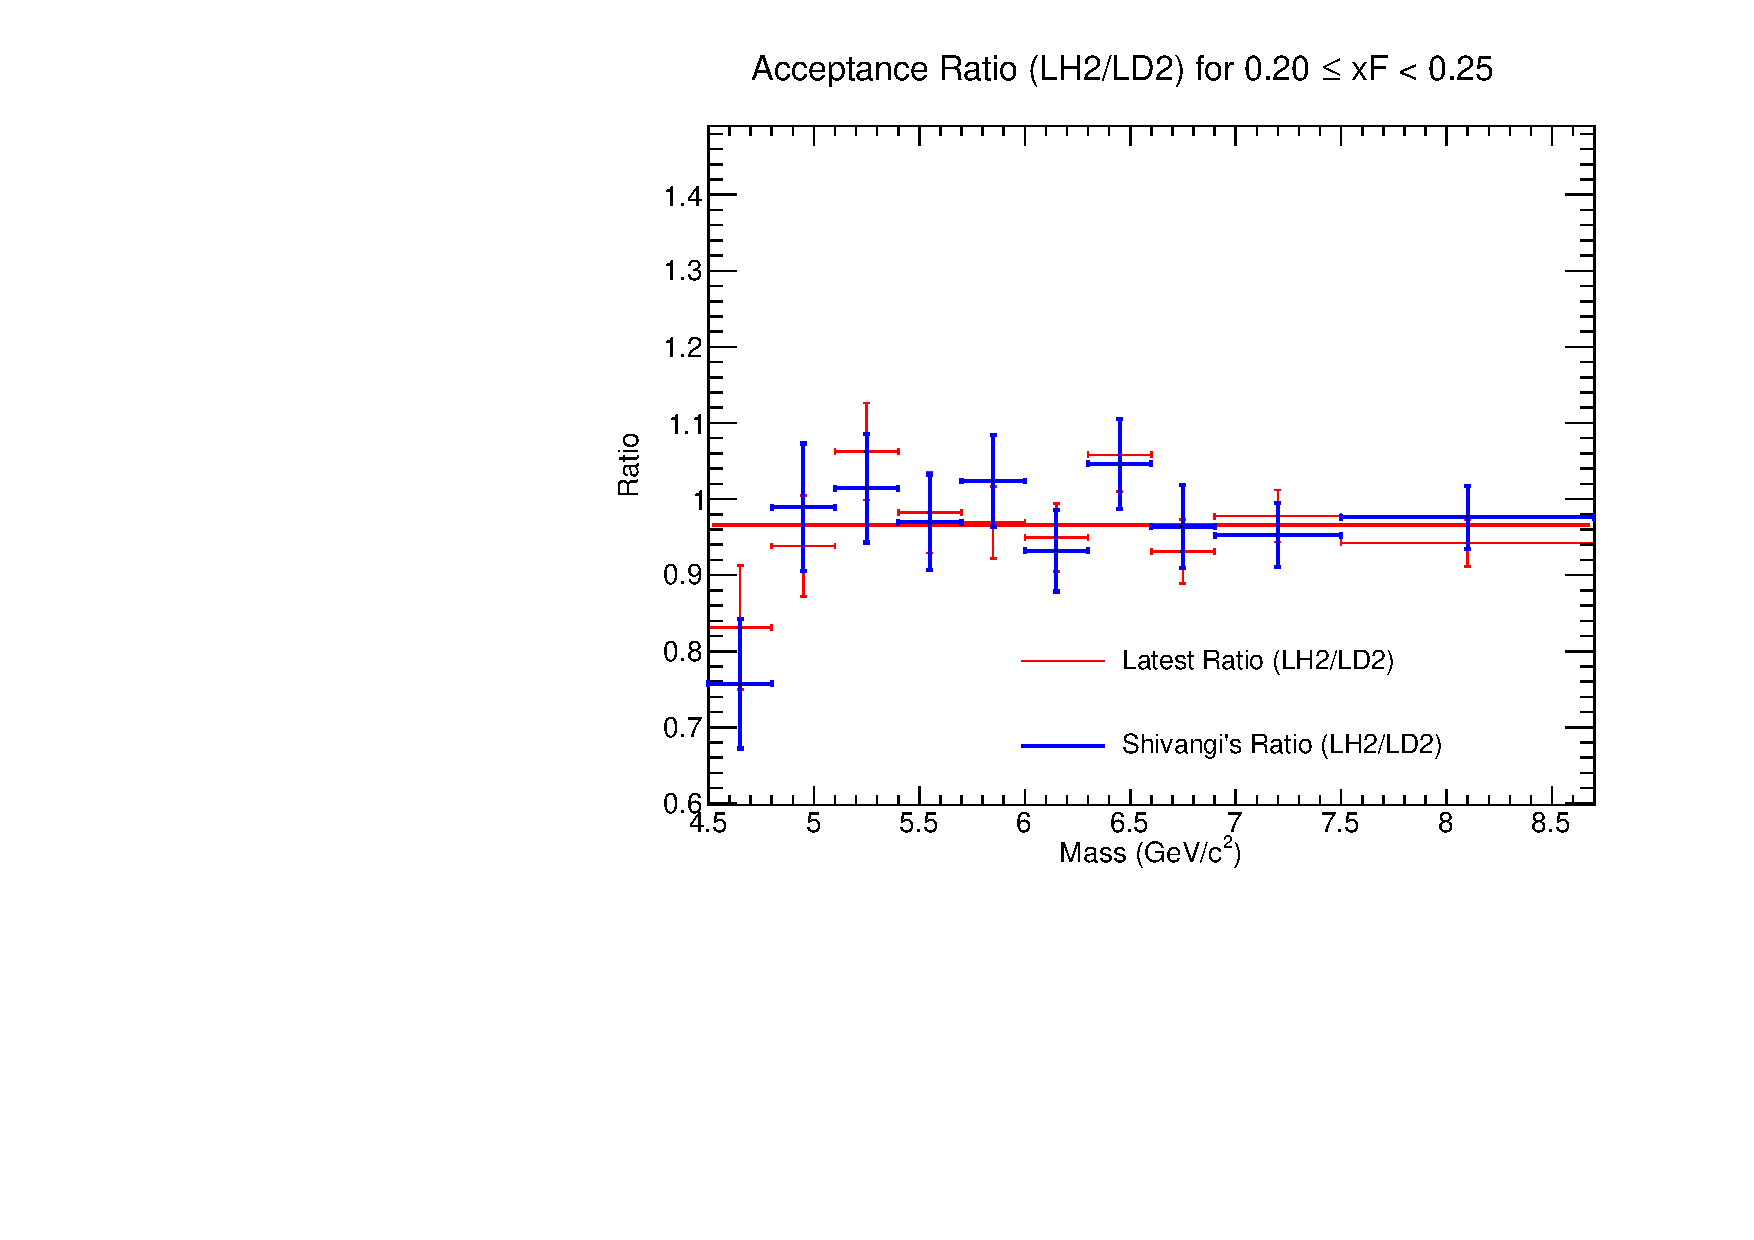
\includegraphics[width=\linewidth]{./acceptancePlots/Acceptance_ratio_xF_bin_4.pdf}
       \caption{Acceptance Ratio (LH2/LD2)}
    \end{subfigure}
    \caption{Acceptance plots for $0.20 \le x_F < 0.25$.}
\end{figure}

\begin{figure}[p]
    \centering
    \begin{subfigure}[b]{0.48\textwidth}
       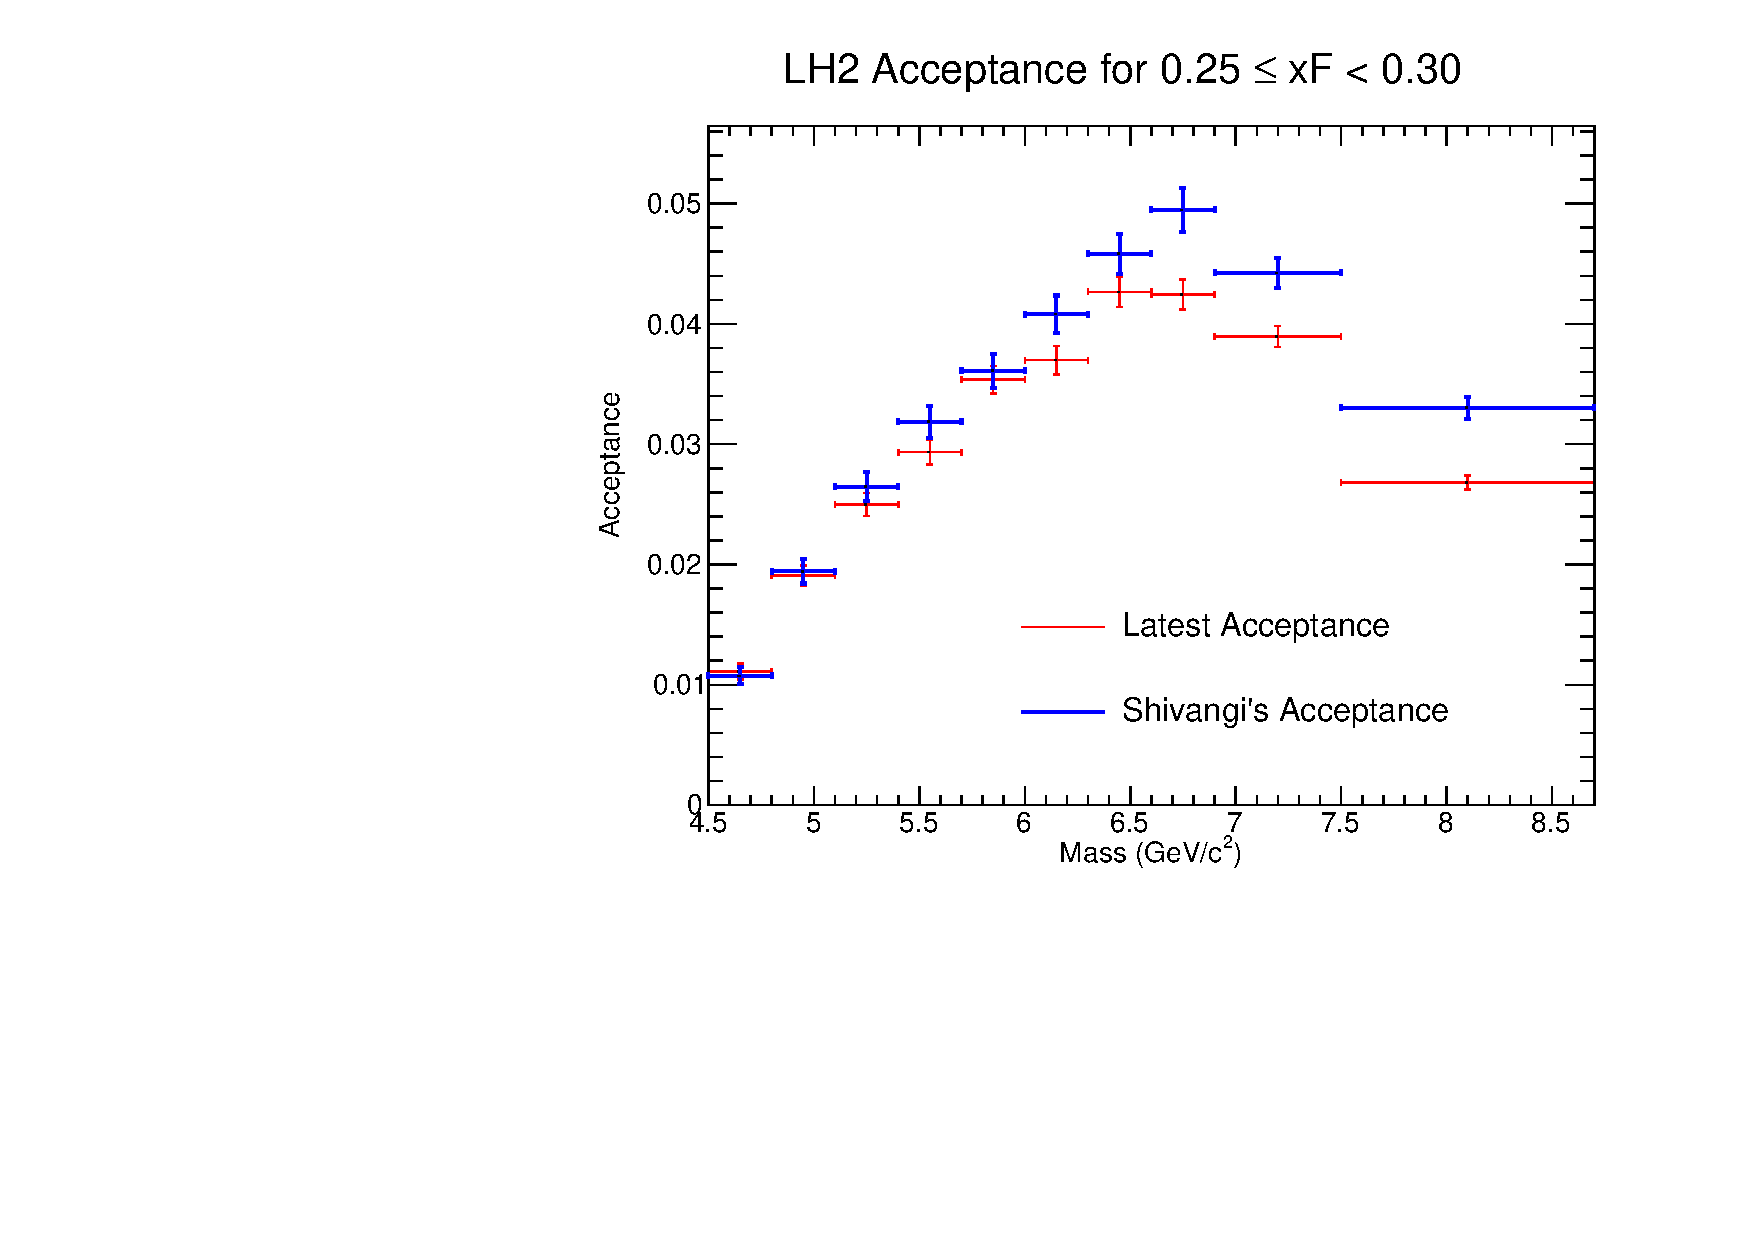
\includegraphics[width=\linewidth]{./acceptancePlots/LH2_acceptance_xF_bin_5.pdf}
       \caption{Acceptance for LH2}
    \end{subfigure}\hfill
    \begin{subfigure}[b]{0.48\textwidth}
       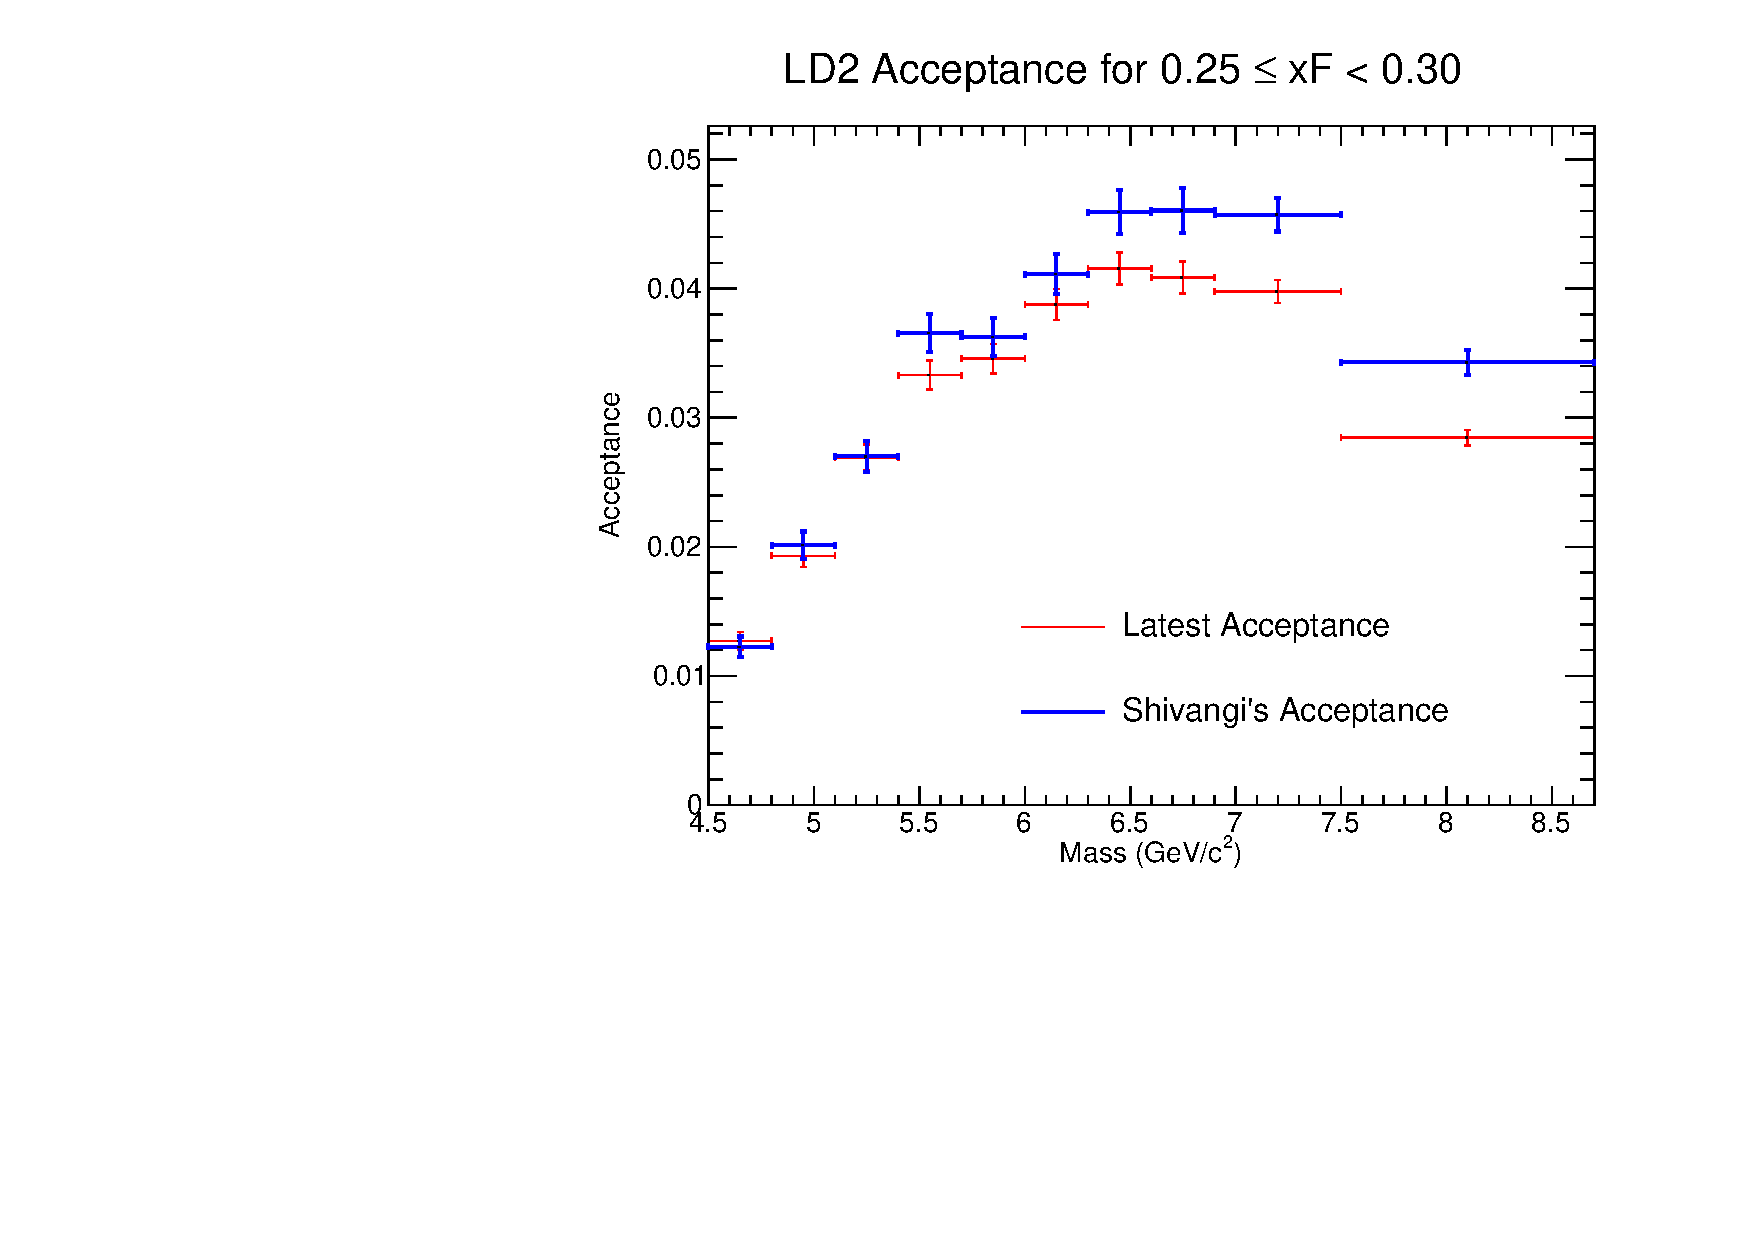
\includegraphics[width=\linewidth]{./acceptancePlots/LD2_acceptance_xF_bin_5.pdf}
       \caption{Acceptance for LD2}
    \end{subfigure}
    \begin{subfigure}[b]{0.48\textwidth}
       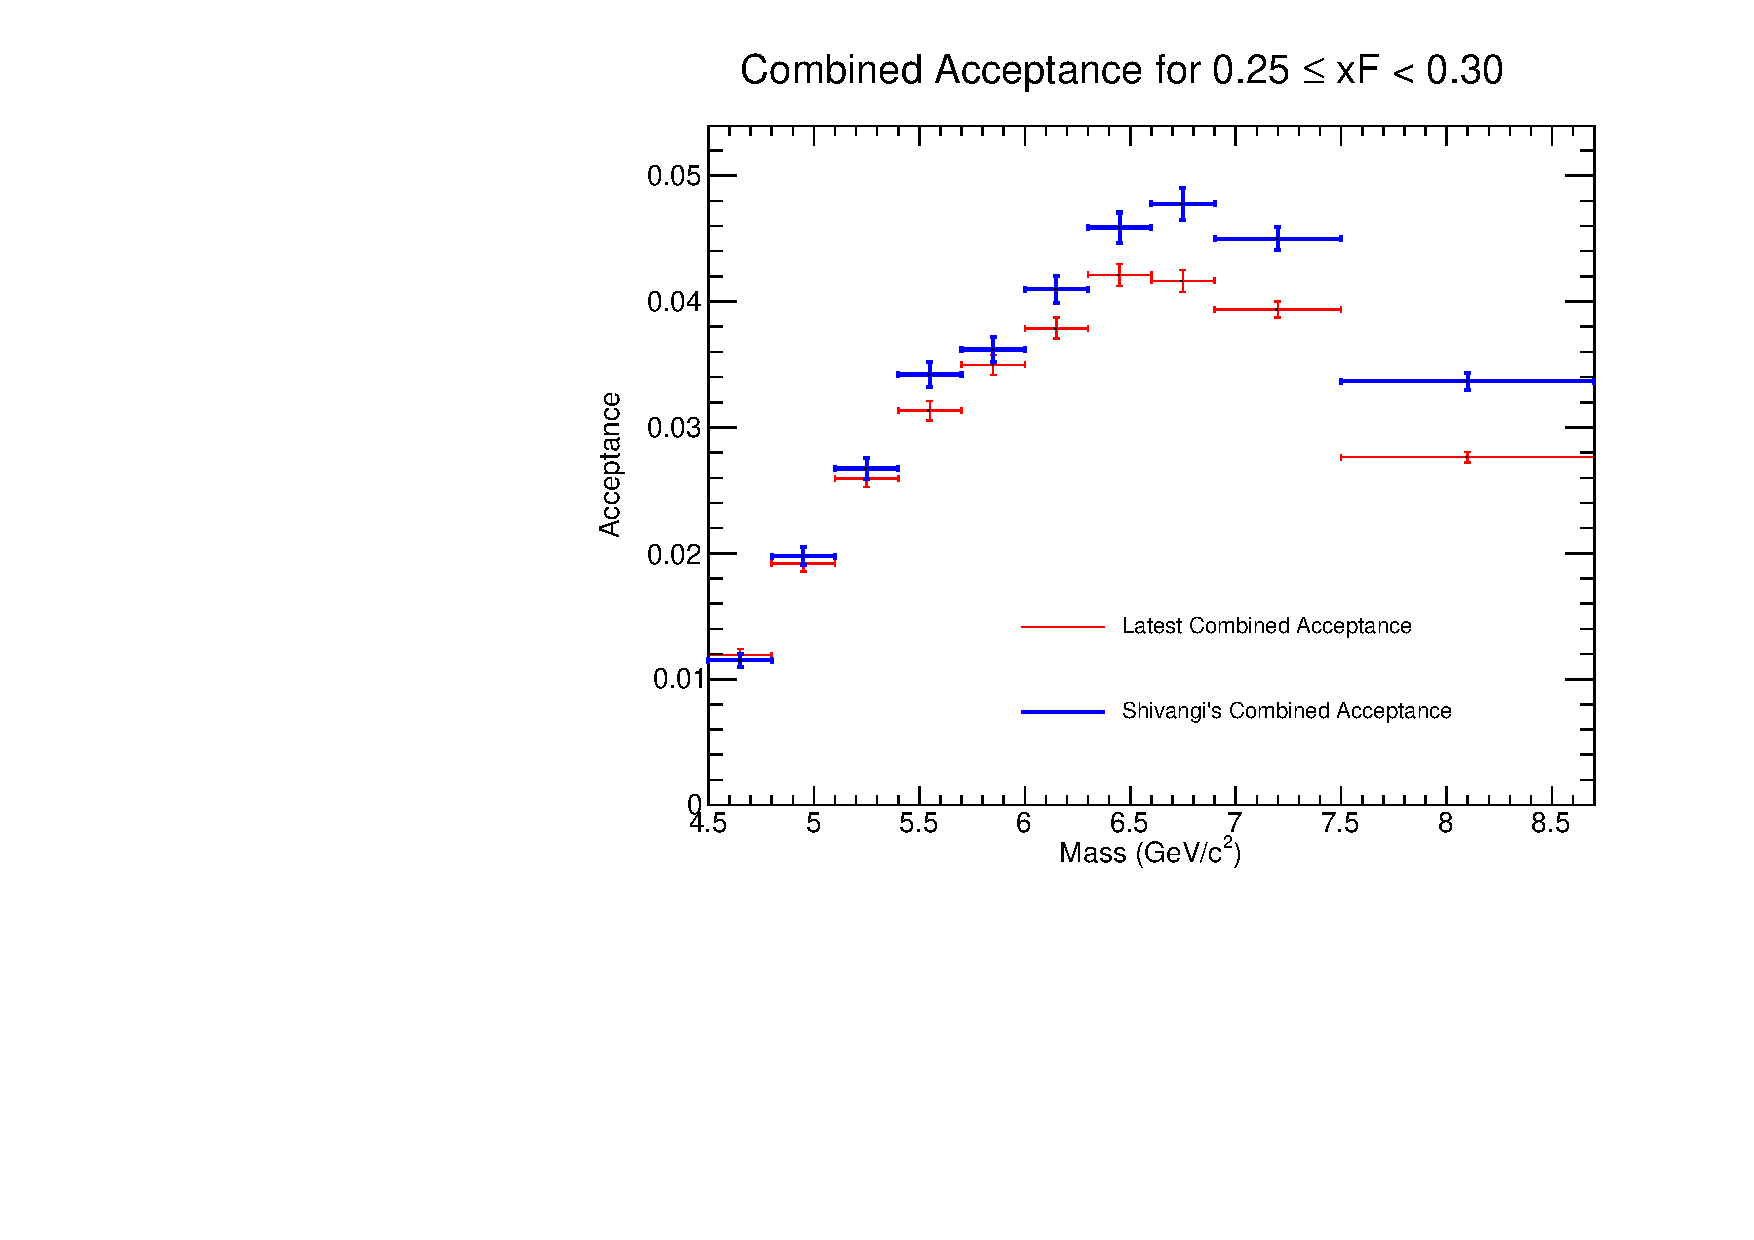
\includegraphics[width=\linewidth]{./acceptancePlots/Combined_acceptance_xF_bin_5.pdf}
       \caption{Combined Acceptance}
    \end{subfigure}\hfill
    \begin{subfigure}[b]{0.48\textwidth}
       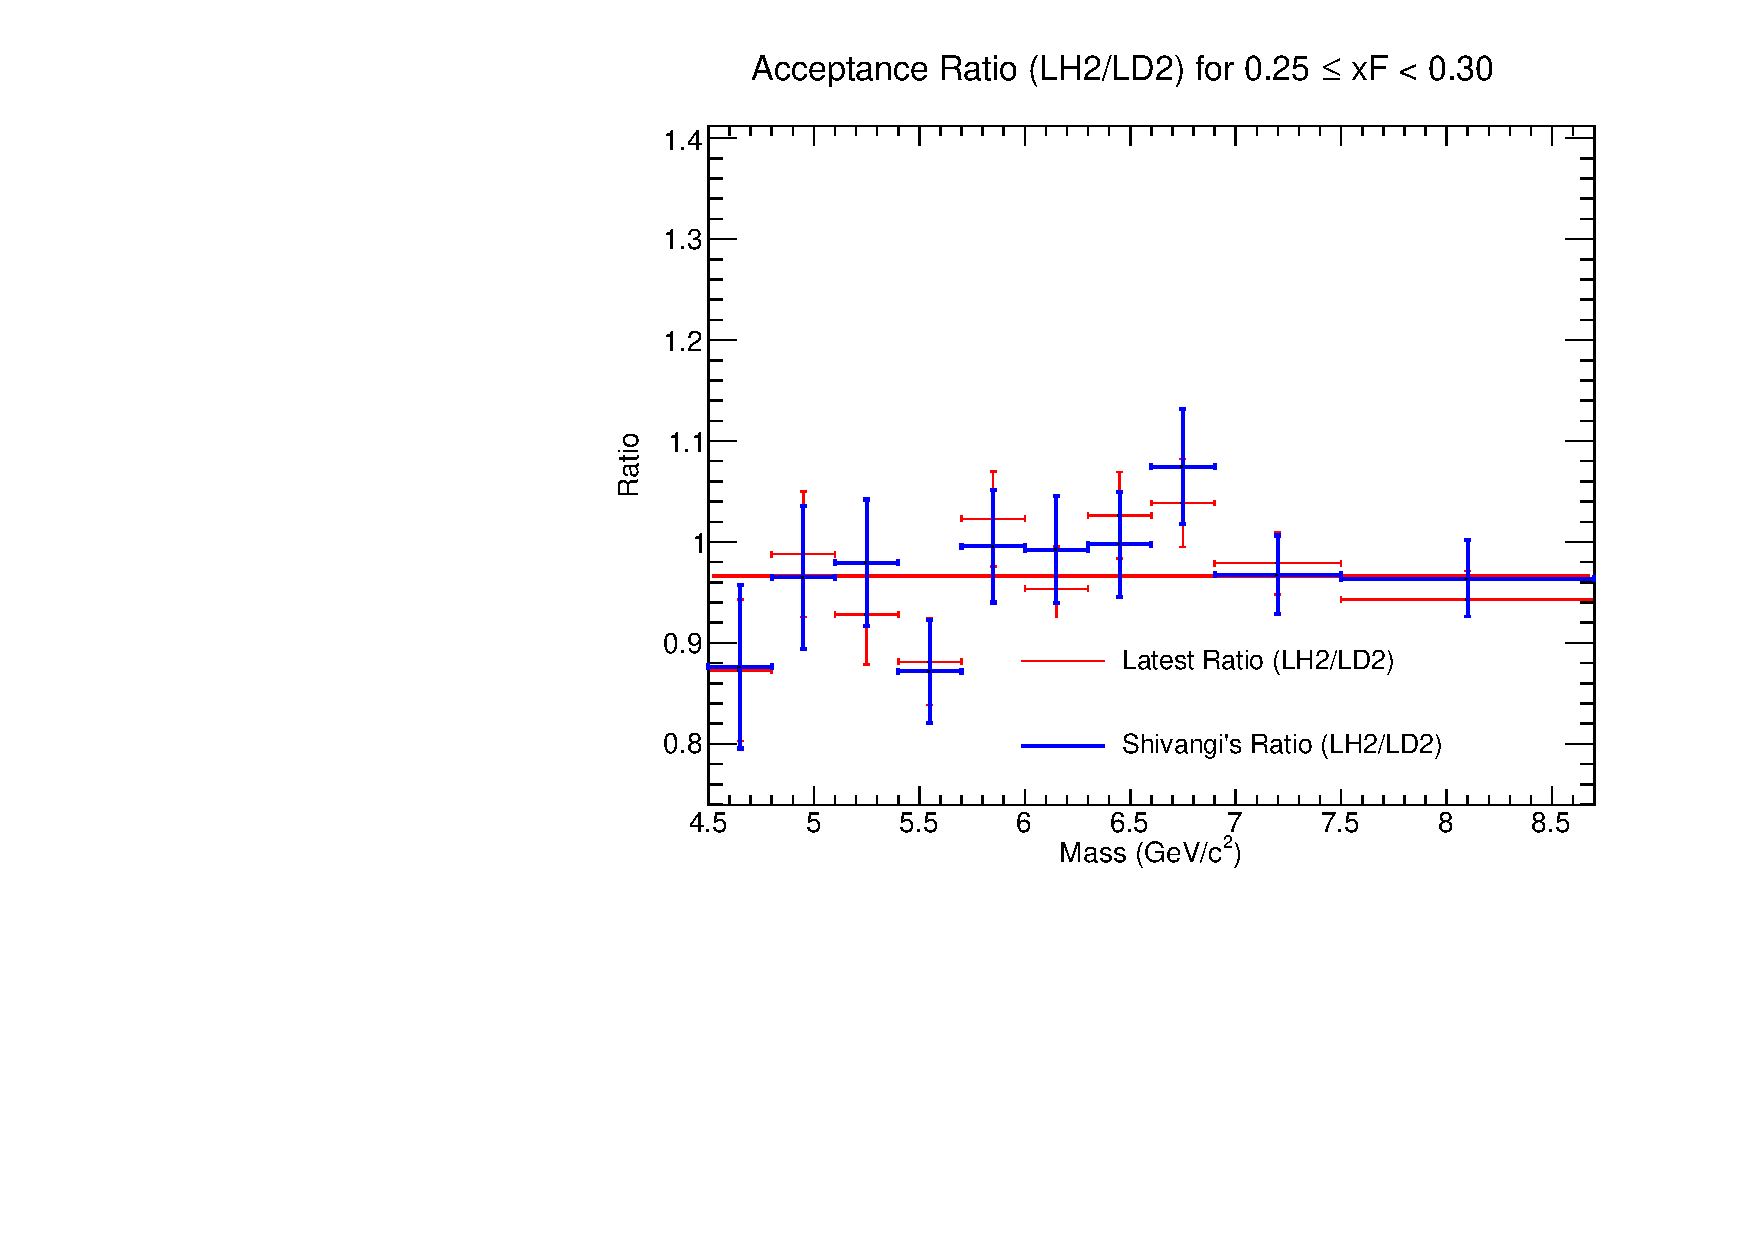
\includegraphics[width=\linewidth]{./acceptancePlots/Acceptance_ratio_xF_bin_5.pdf}
       \caption{Acceptance Ratio (LH2/LD2)}
    \end{subfigure}
    \caption{Acceptance plots for $0.25 \le x_F < 0.30$.}
\end{figure}

\begin{figure}[p]
    \centering
    \begin{subfigure}[b]{0.48\textwidth}
       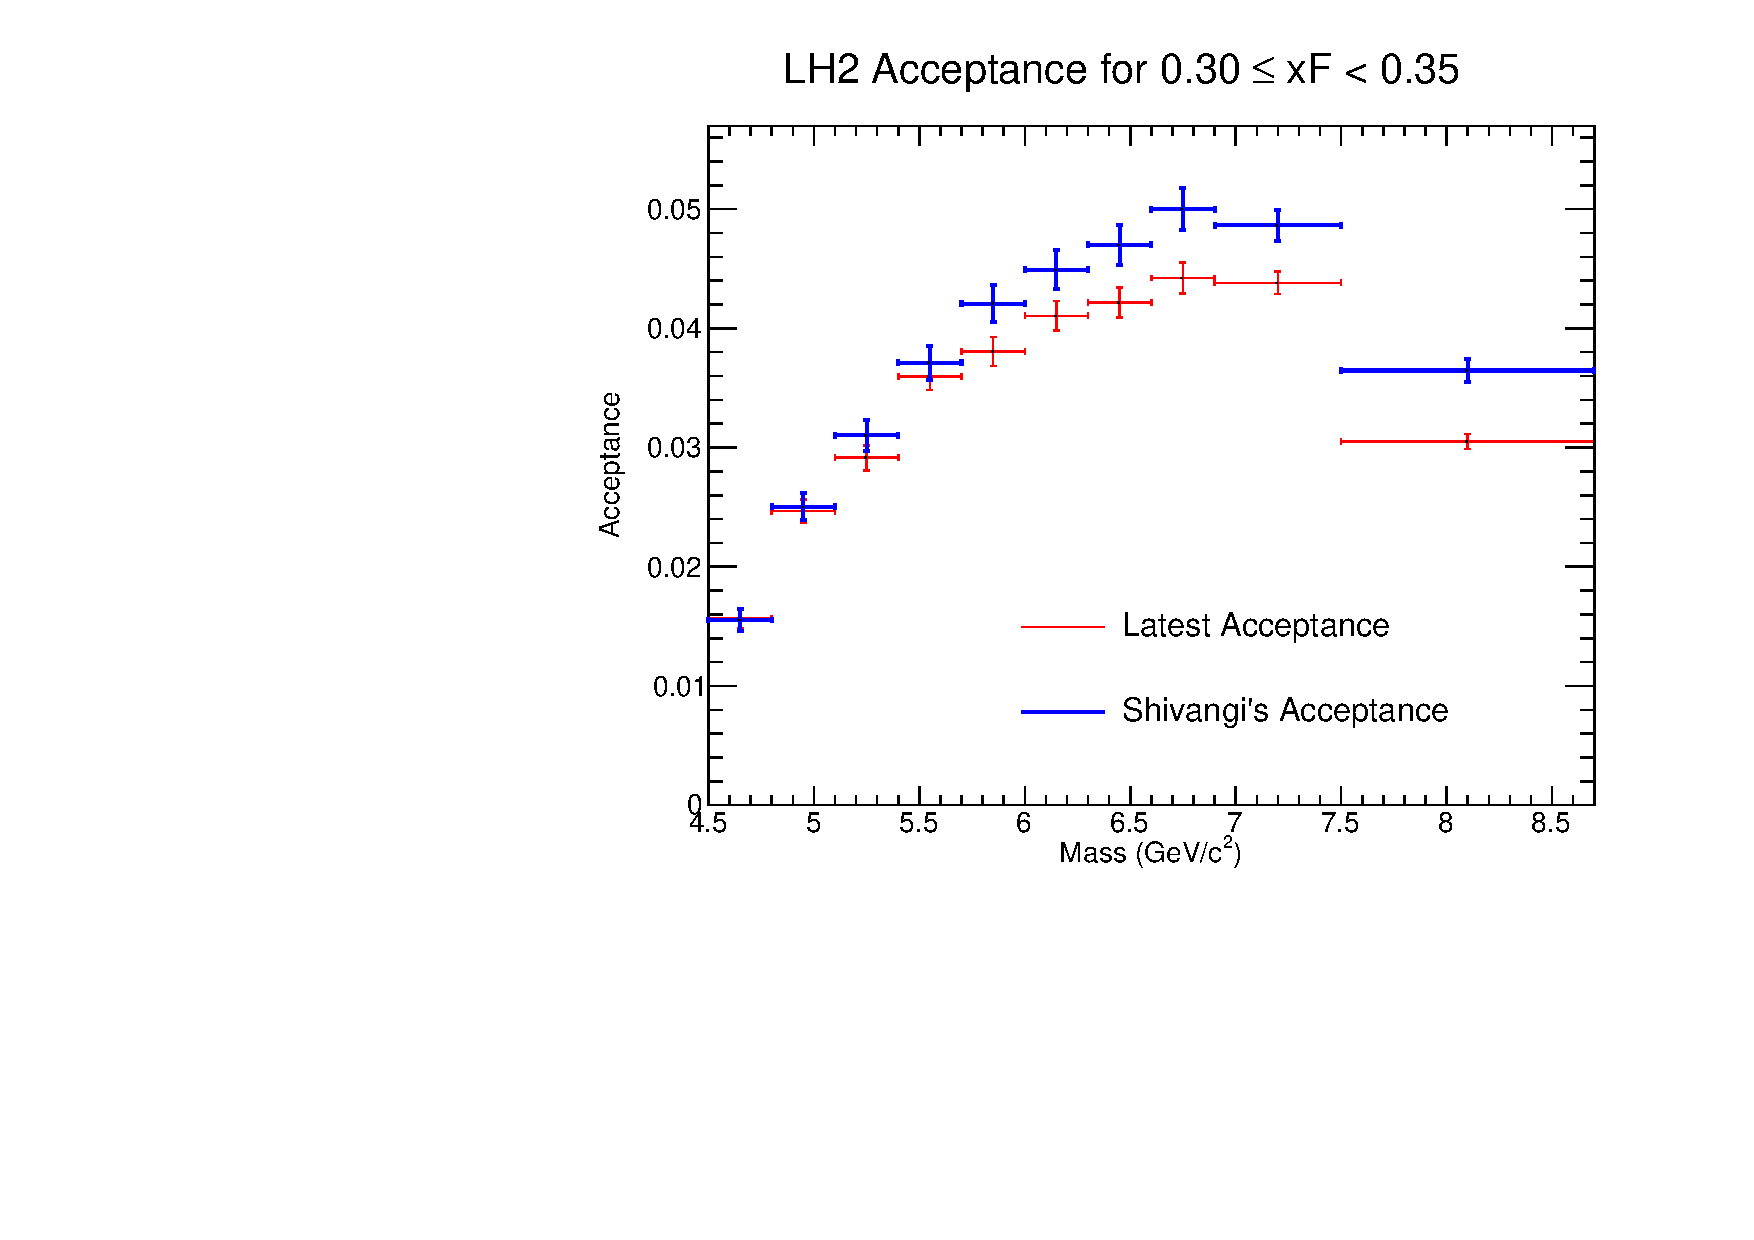
\includegraphics[width=\linewidth]{./acceptancePlots/LH2_acceptance_xF_bin_6.pdf}
       \caption{Acceptance for LH2}
    \end{subfigure}\hfill
    \begin{subfigure}[b]{0.48\textwidth}
       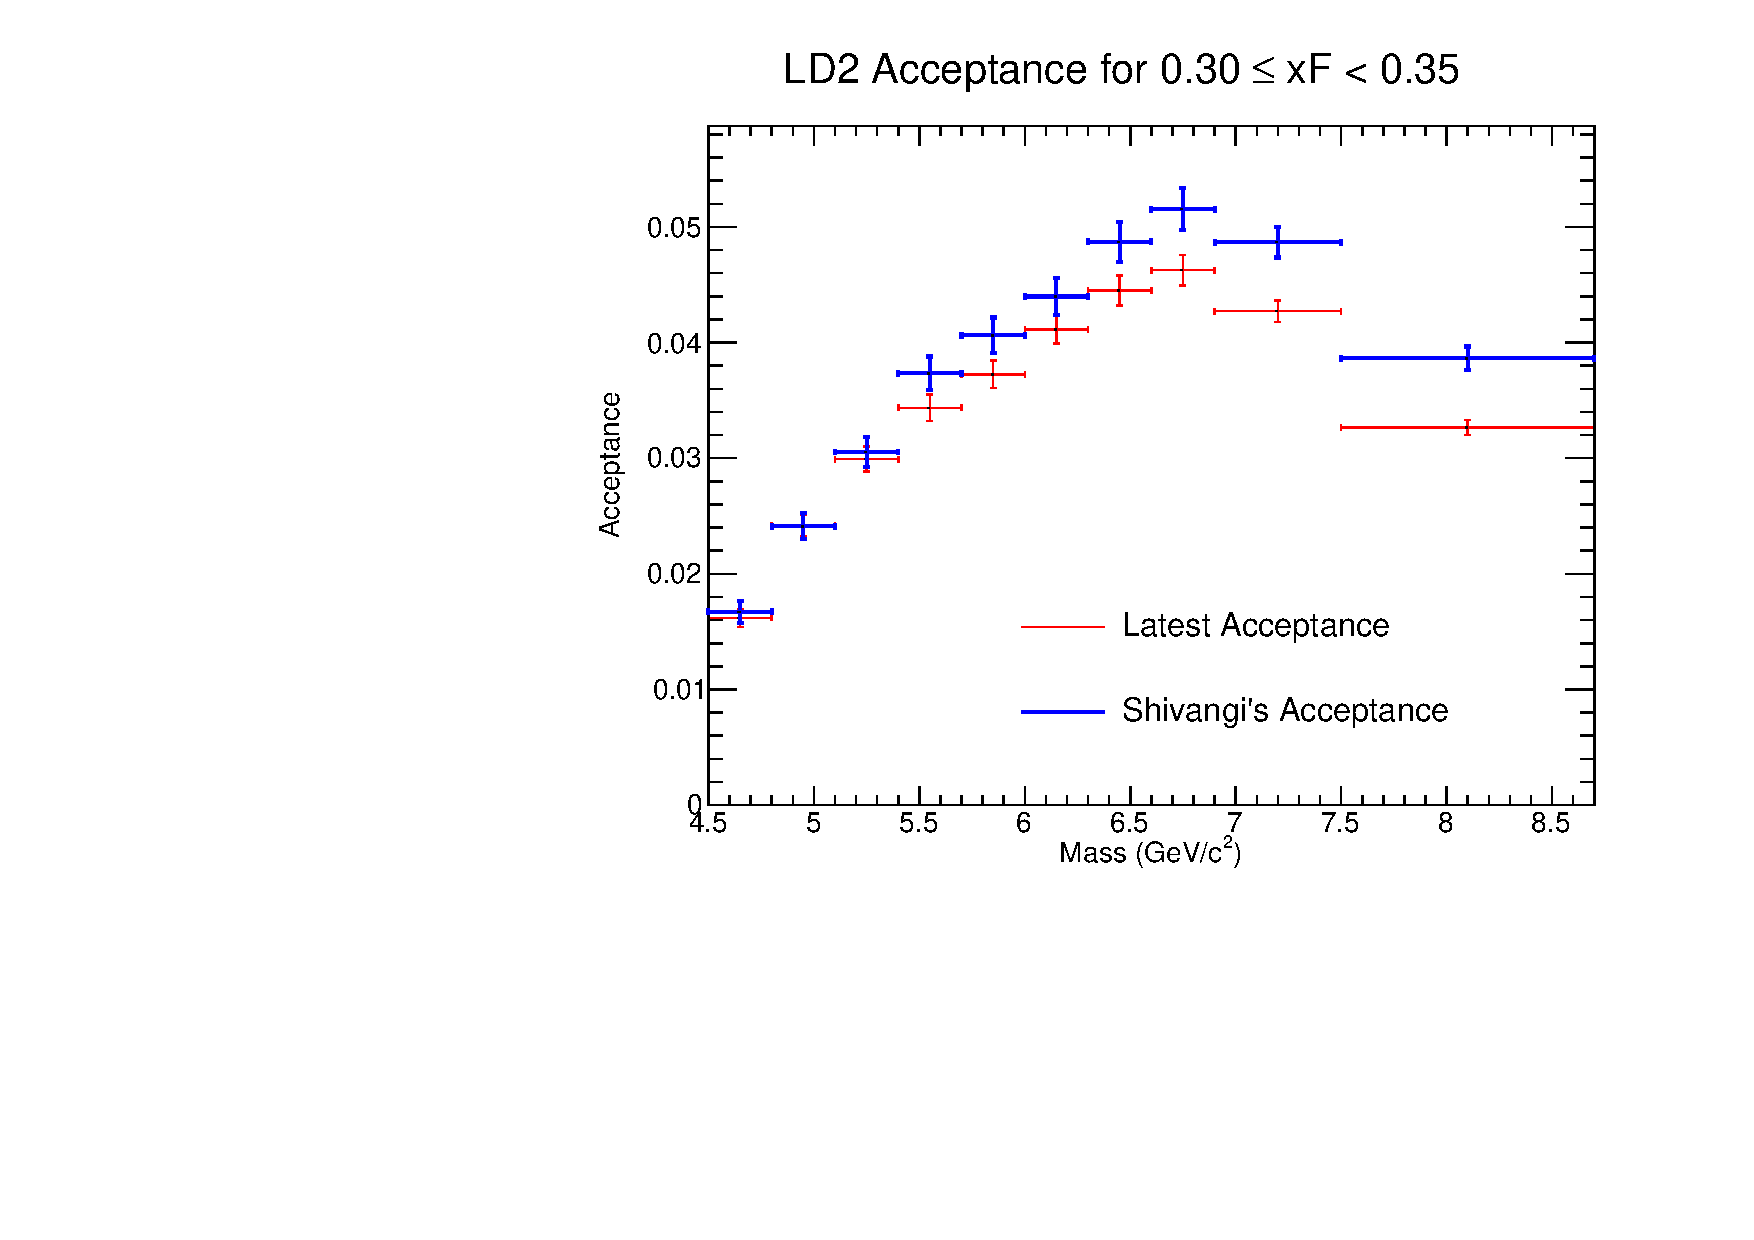
\includegraphics[width=\linewidth]{./acceptancePlots/LD2_acceptance_xF_bin_6.pdf}
       \caption{Acceptance for LD2}
    \end{subfigure}
    \begin{subfigure}[b]{0.48\textwidth}
       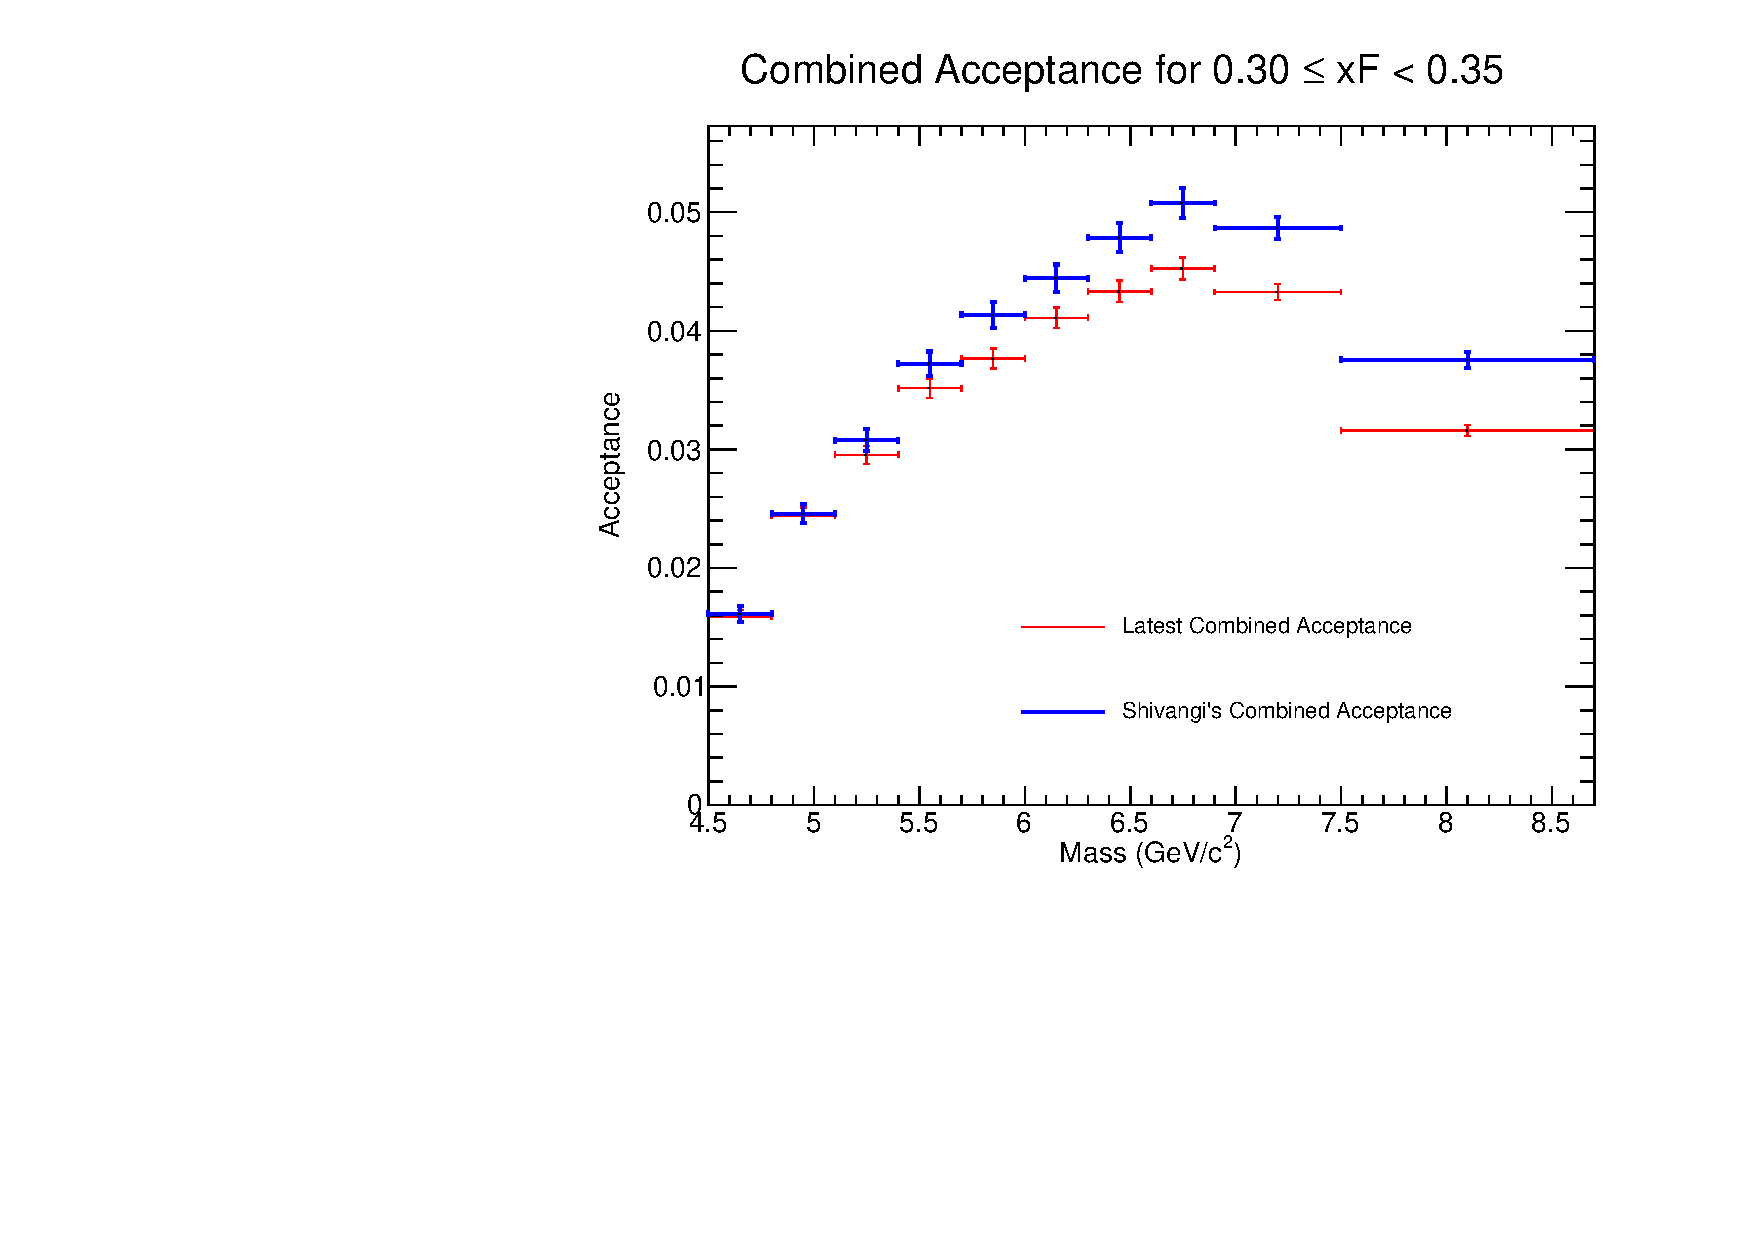
\includegraphics[width=\linewidth]{./acceptancePlots/Combined_acceptance_xF_bin_6.pdf}
       \caption{Combined Acceptance}
    \end{subfigure}\hfill
    \begin{subfigure}[b]{0.48\textwidth}
       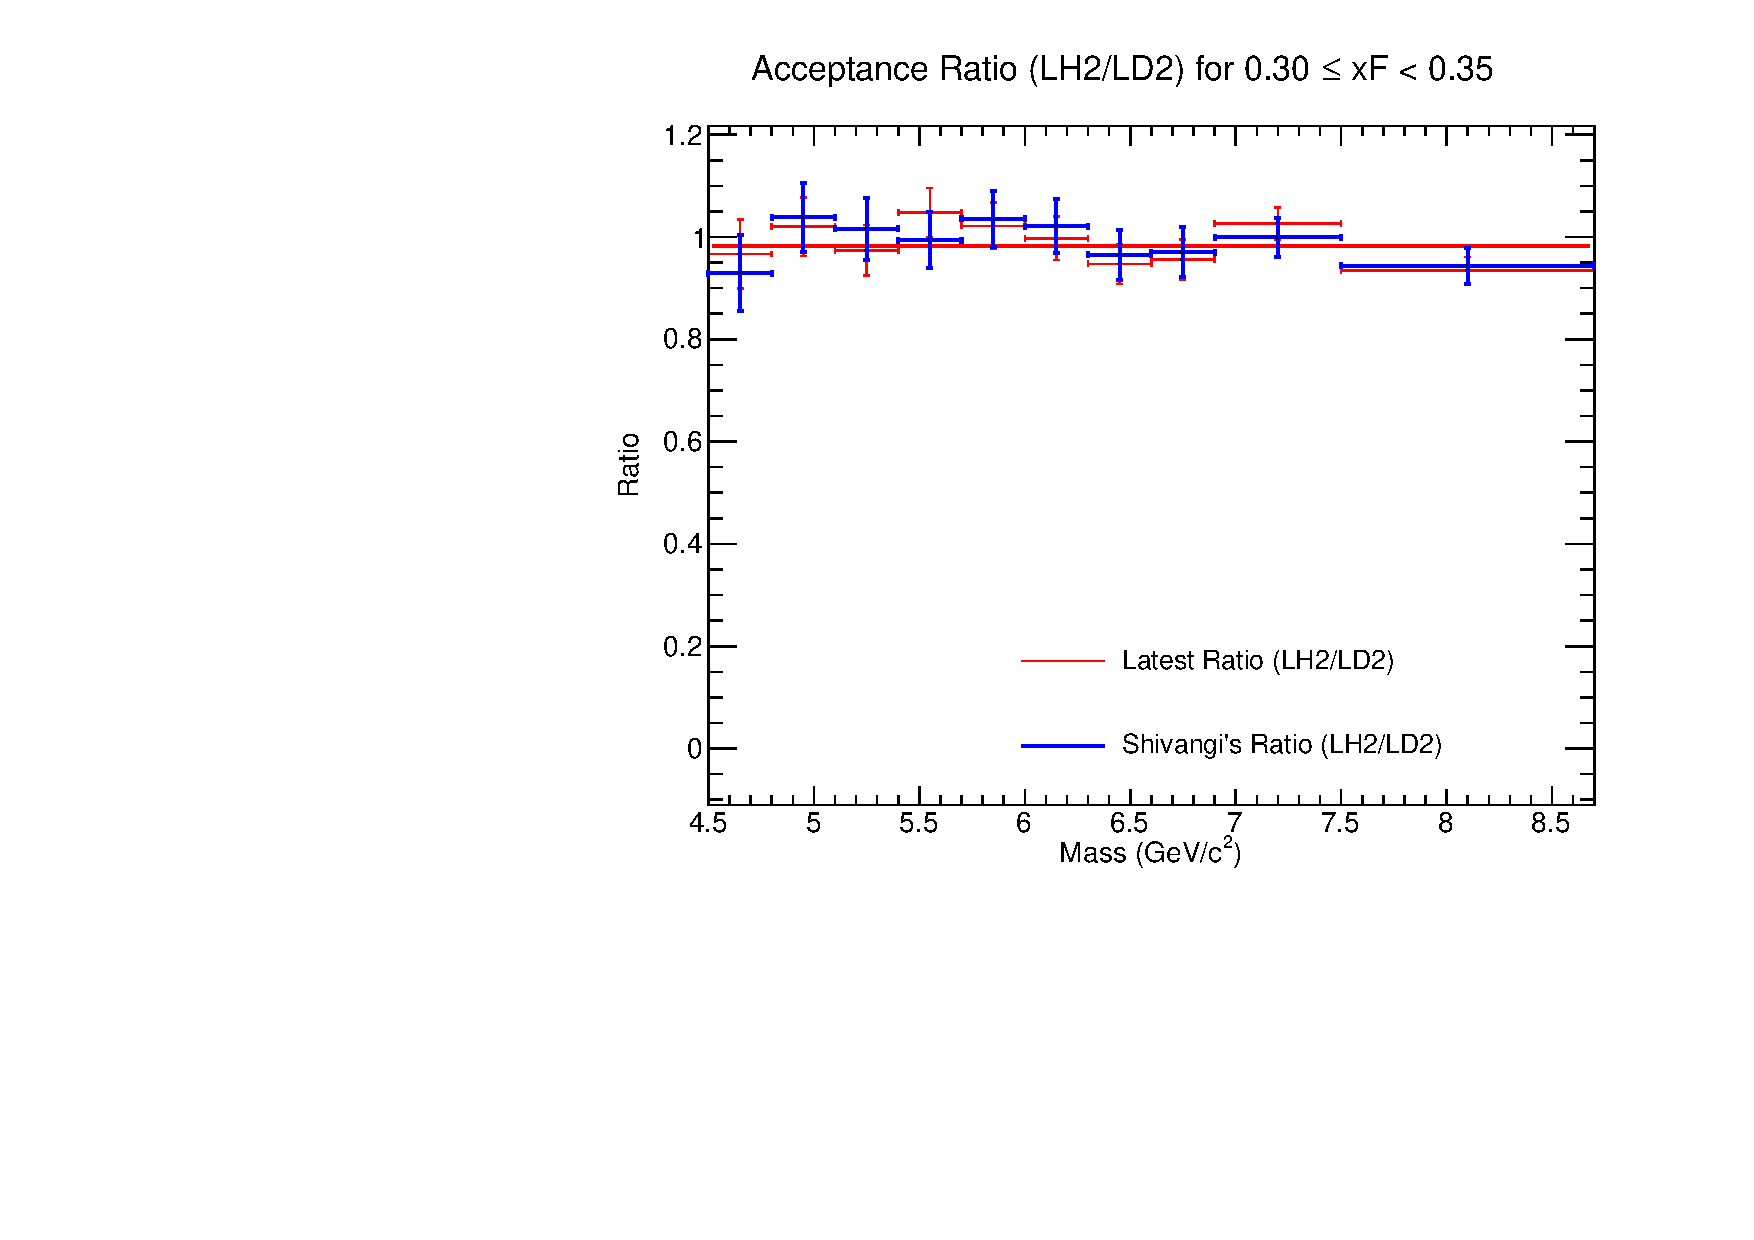
\includegraphics[width=\linewidth]{./acceptancePlots/Acceptance_ratio_xF_bin_6.pdf}
       \caption{Acceptance Ratio (LH2/LD2)}
    \end{subfigure}
    \caption{Acceptance plots for $0.30 \le x_F < 0.35$.}
\end{figure}

\begin{figure}[p]
    \centering
    \begin{subfigure}[b]{0.48\textwidth}
       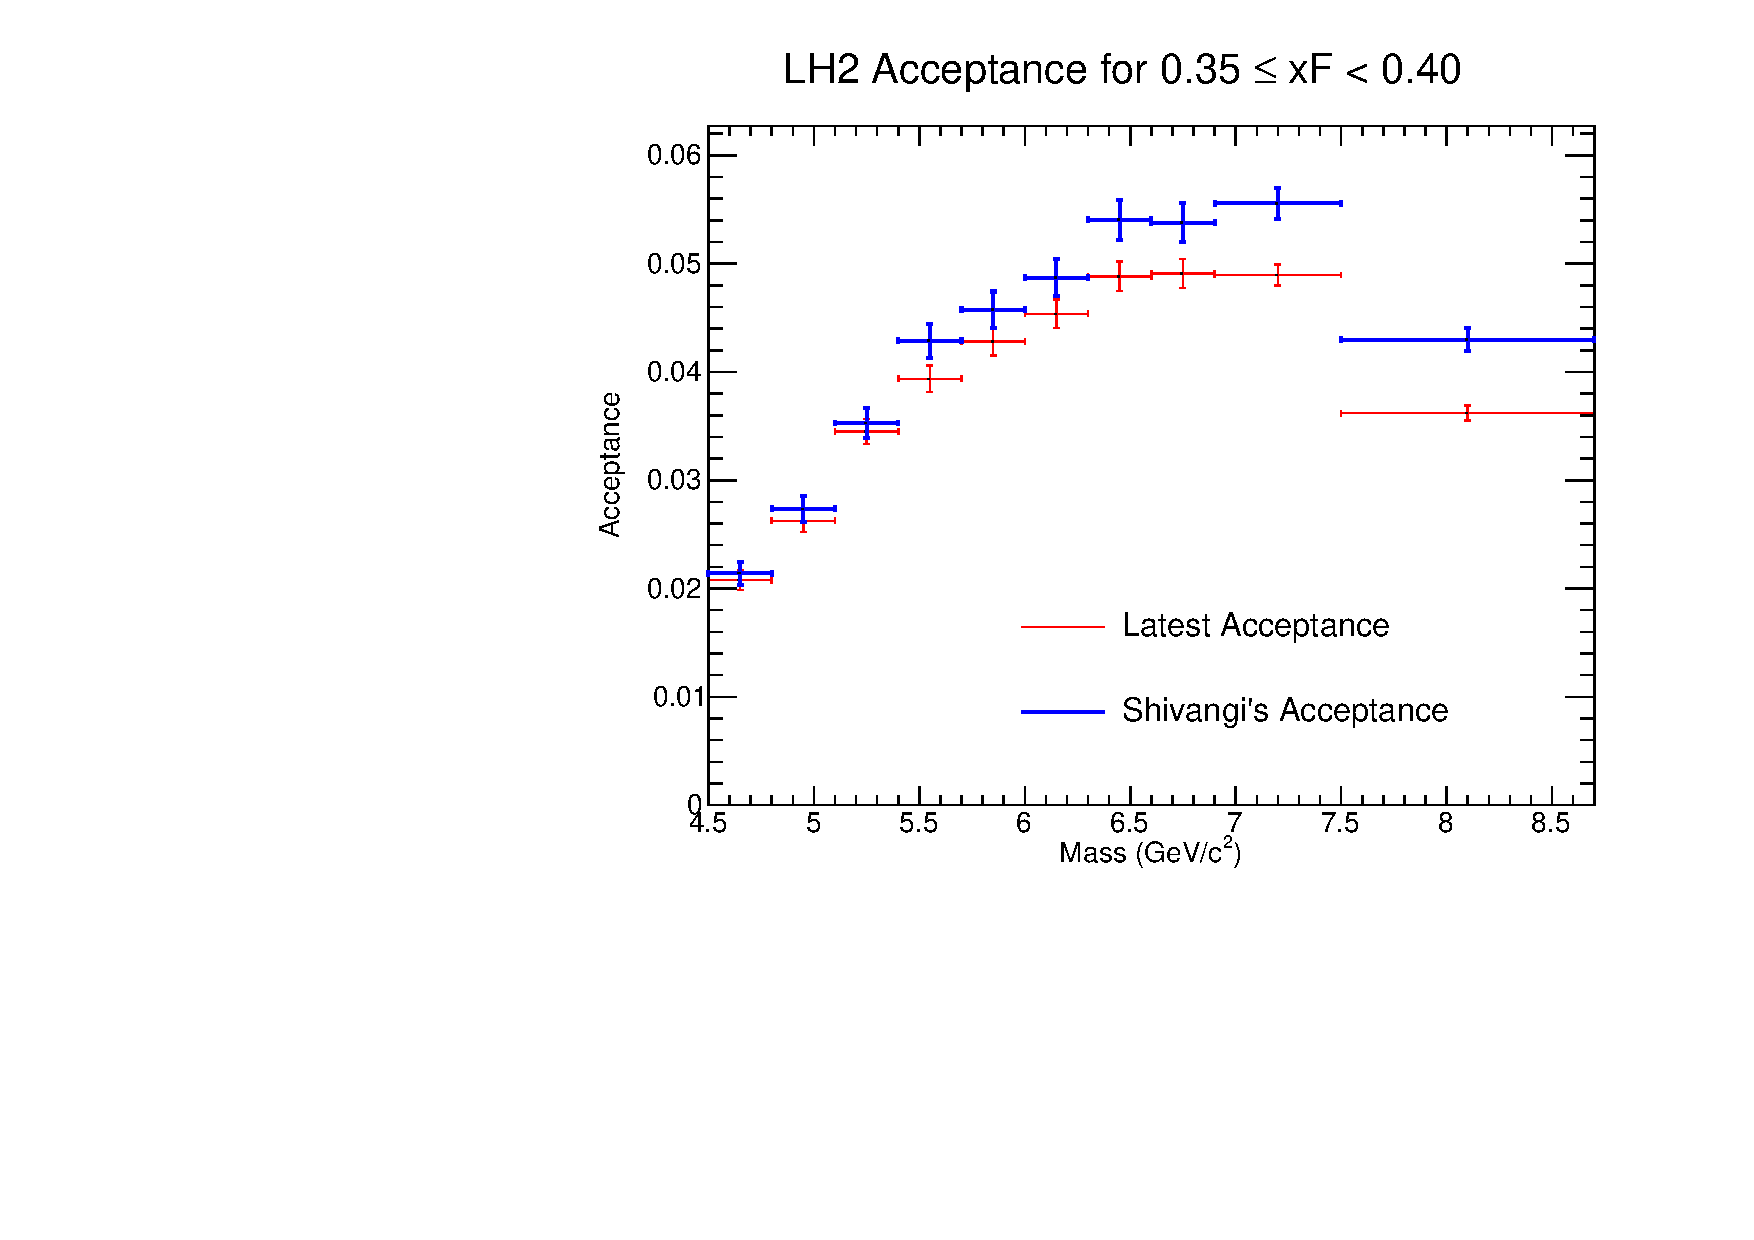
\includegraphics[width=\linewidth]{./acceptancePlots/LH2_acceptance_xF_bin_7.pdf}
       \caption{Acceptance for LH2}
    \end{subfigure}\hfill
    \begin{subfigure}[b]{0.48\textwidth}
       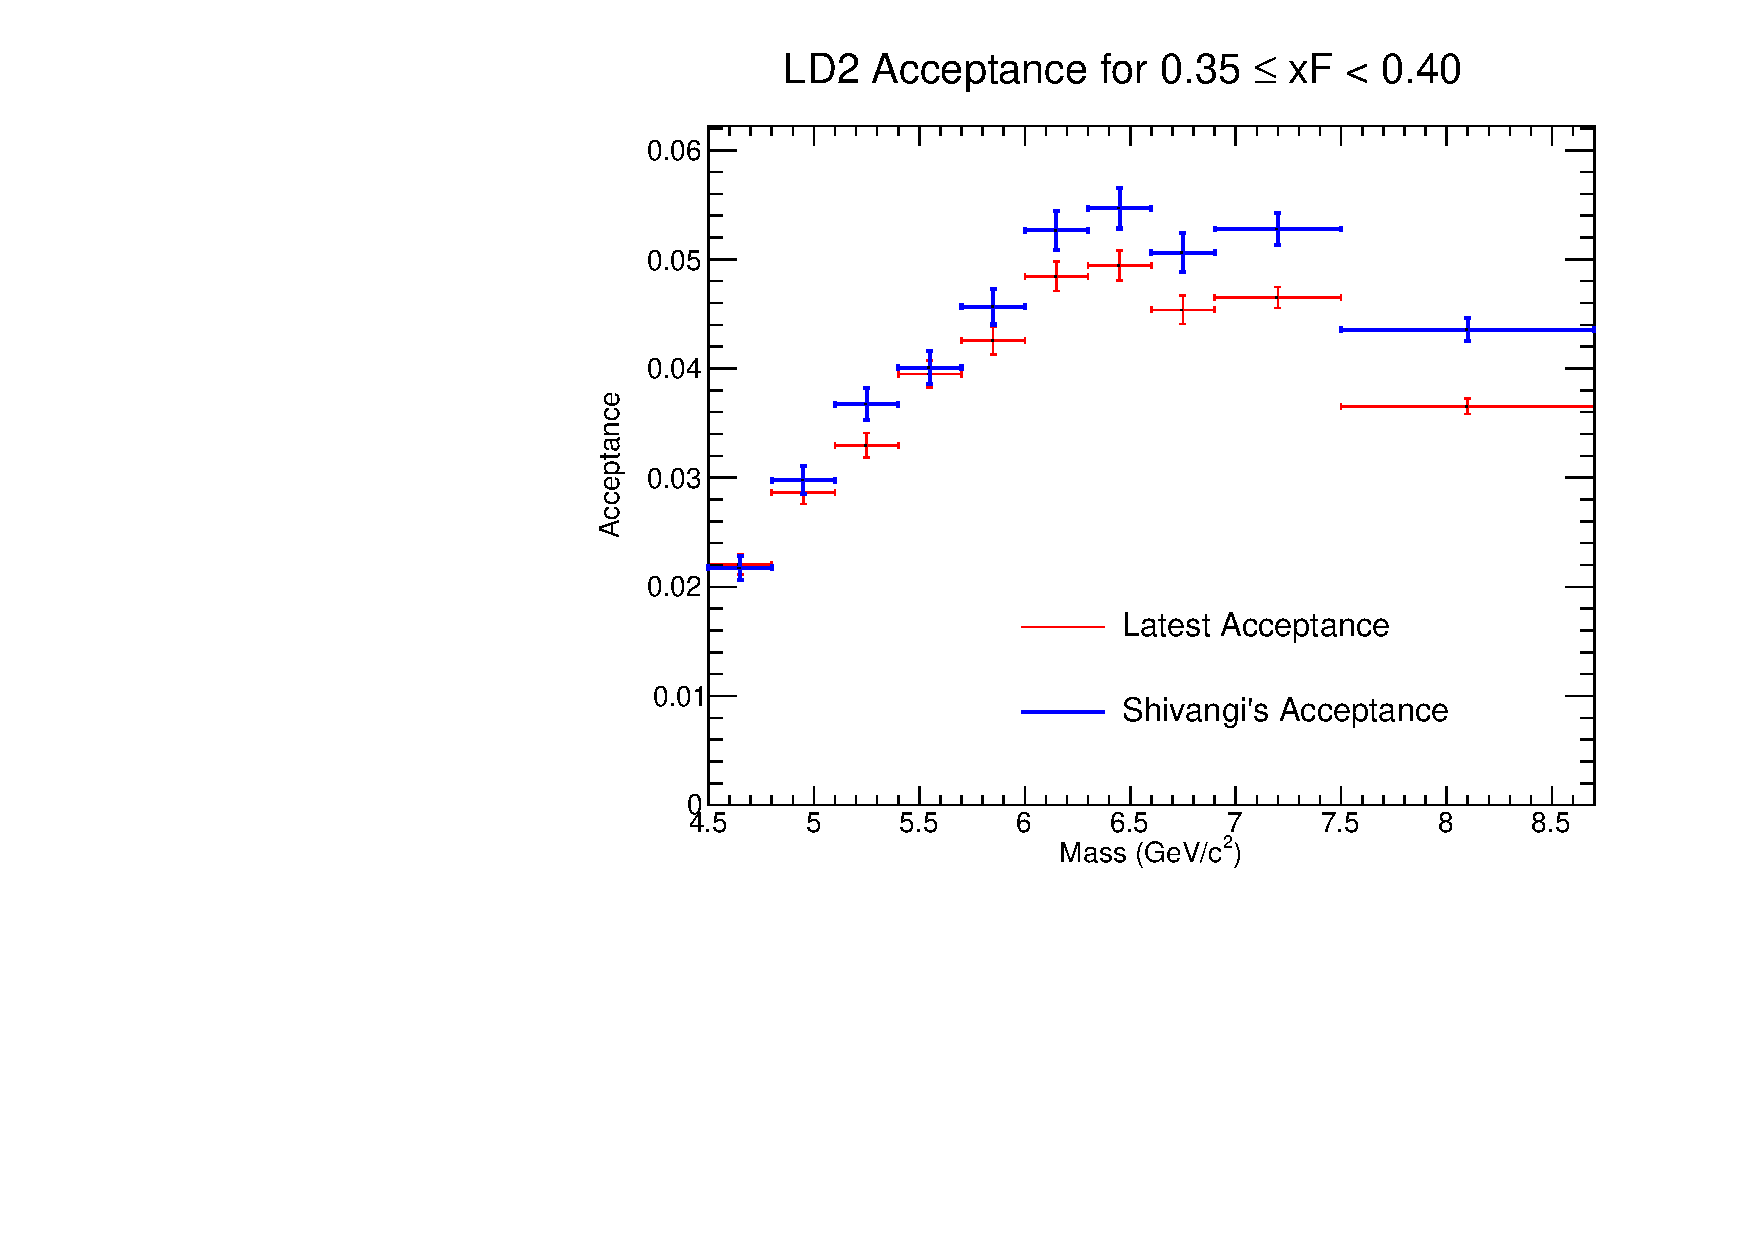
\includegraphics[width=\linewidth]{./acceptancePlots/LD2_acceptance_xF_bin_7.pdf}
       \caption{Acceptance for LD2}
    \end{subfigure}
    \begin{subfigure}[b]{0.48\textwidth}
       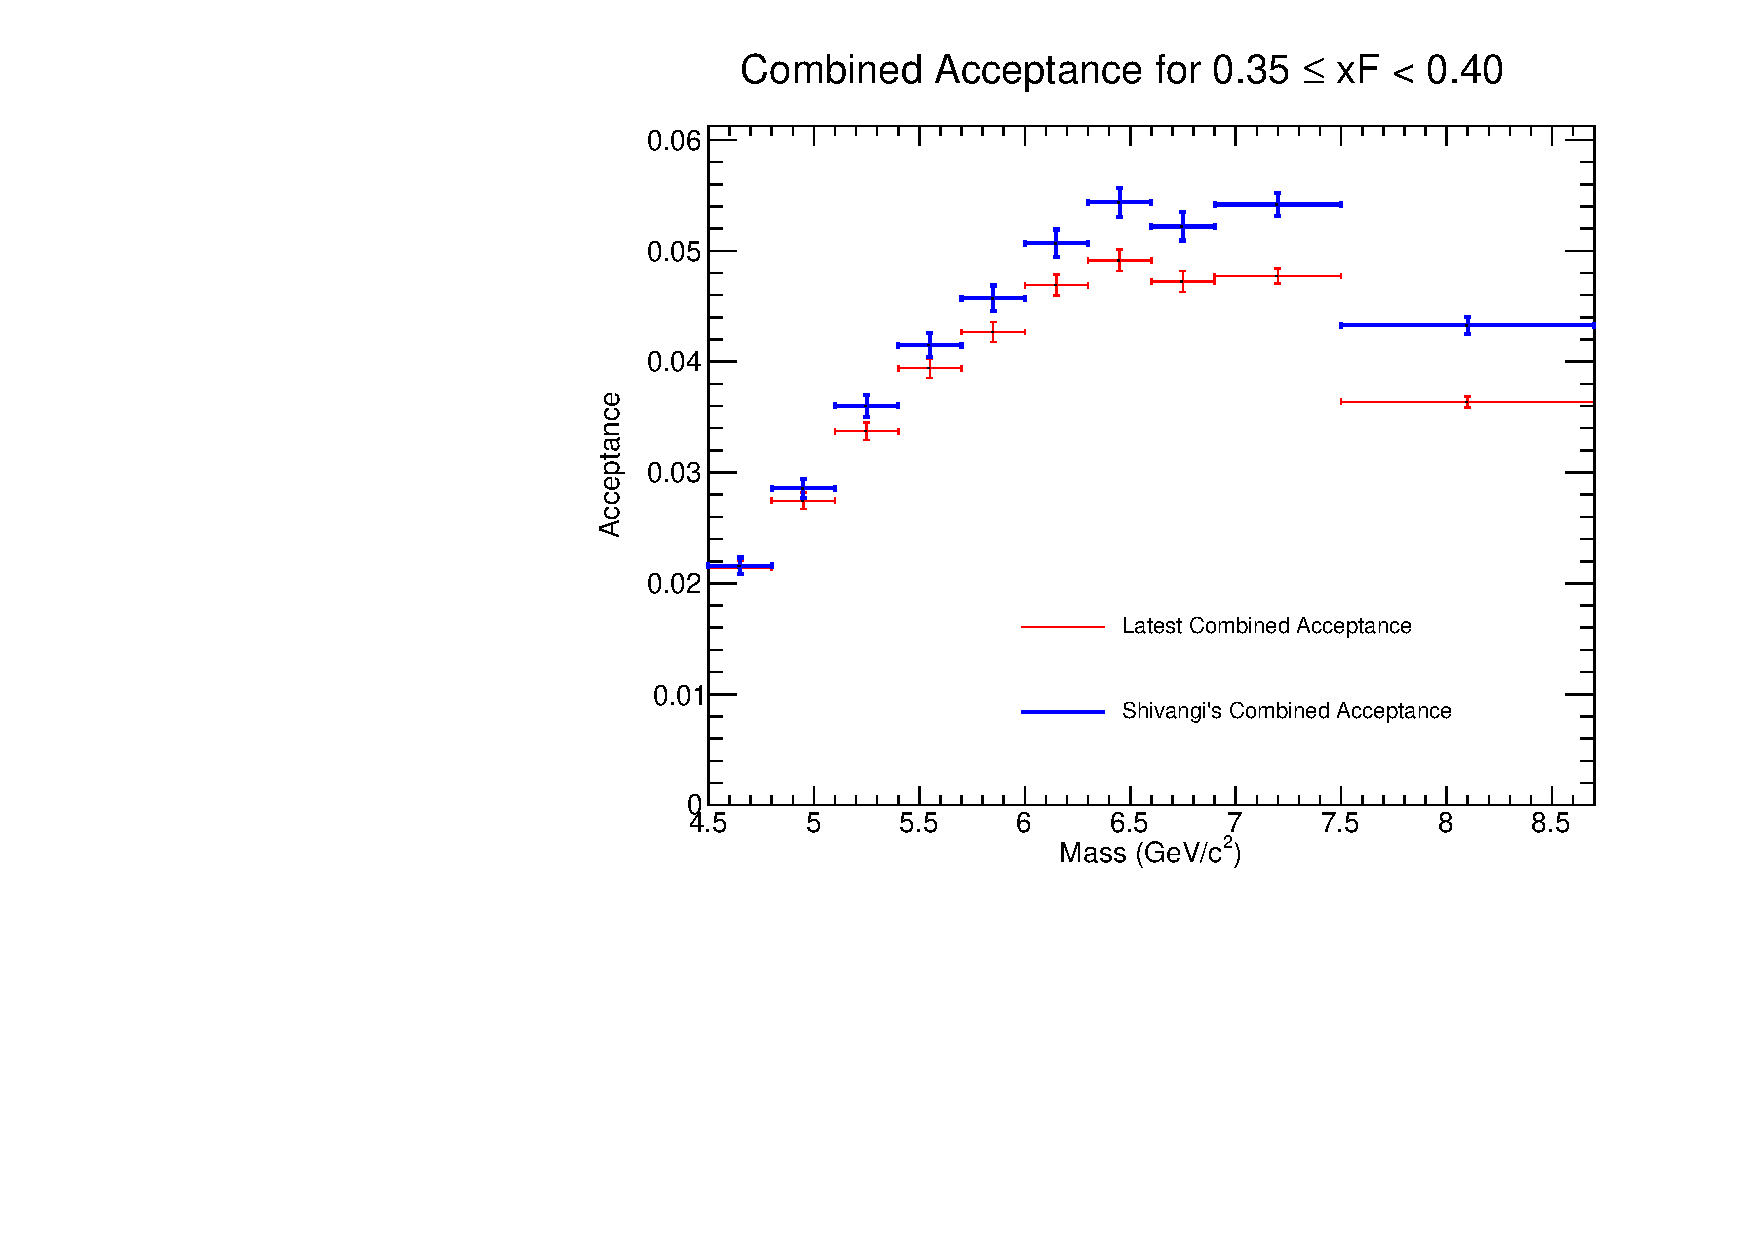
\includegraphics[width=\linewidth]{./acceptancePlots/Combined_acceptance_xF_bin_7.pdf}
       \caption{Combined Acceptance}
    \end{subfigure}\hfill
    \begin{subfigure}[b]{0.48\textwidth}
       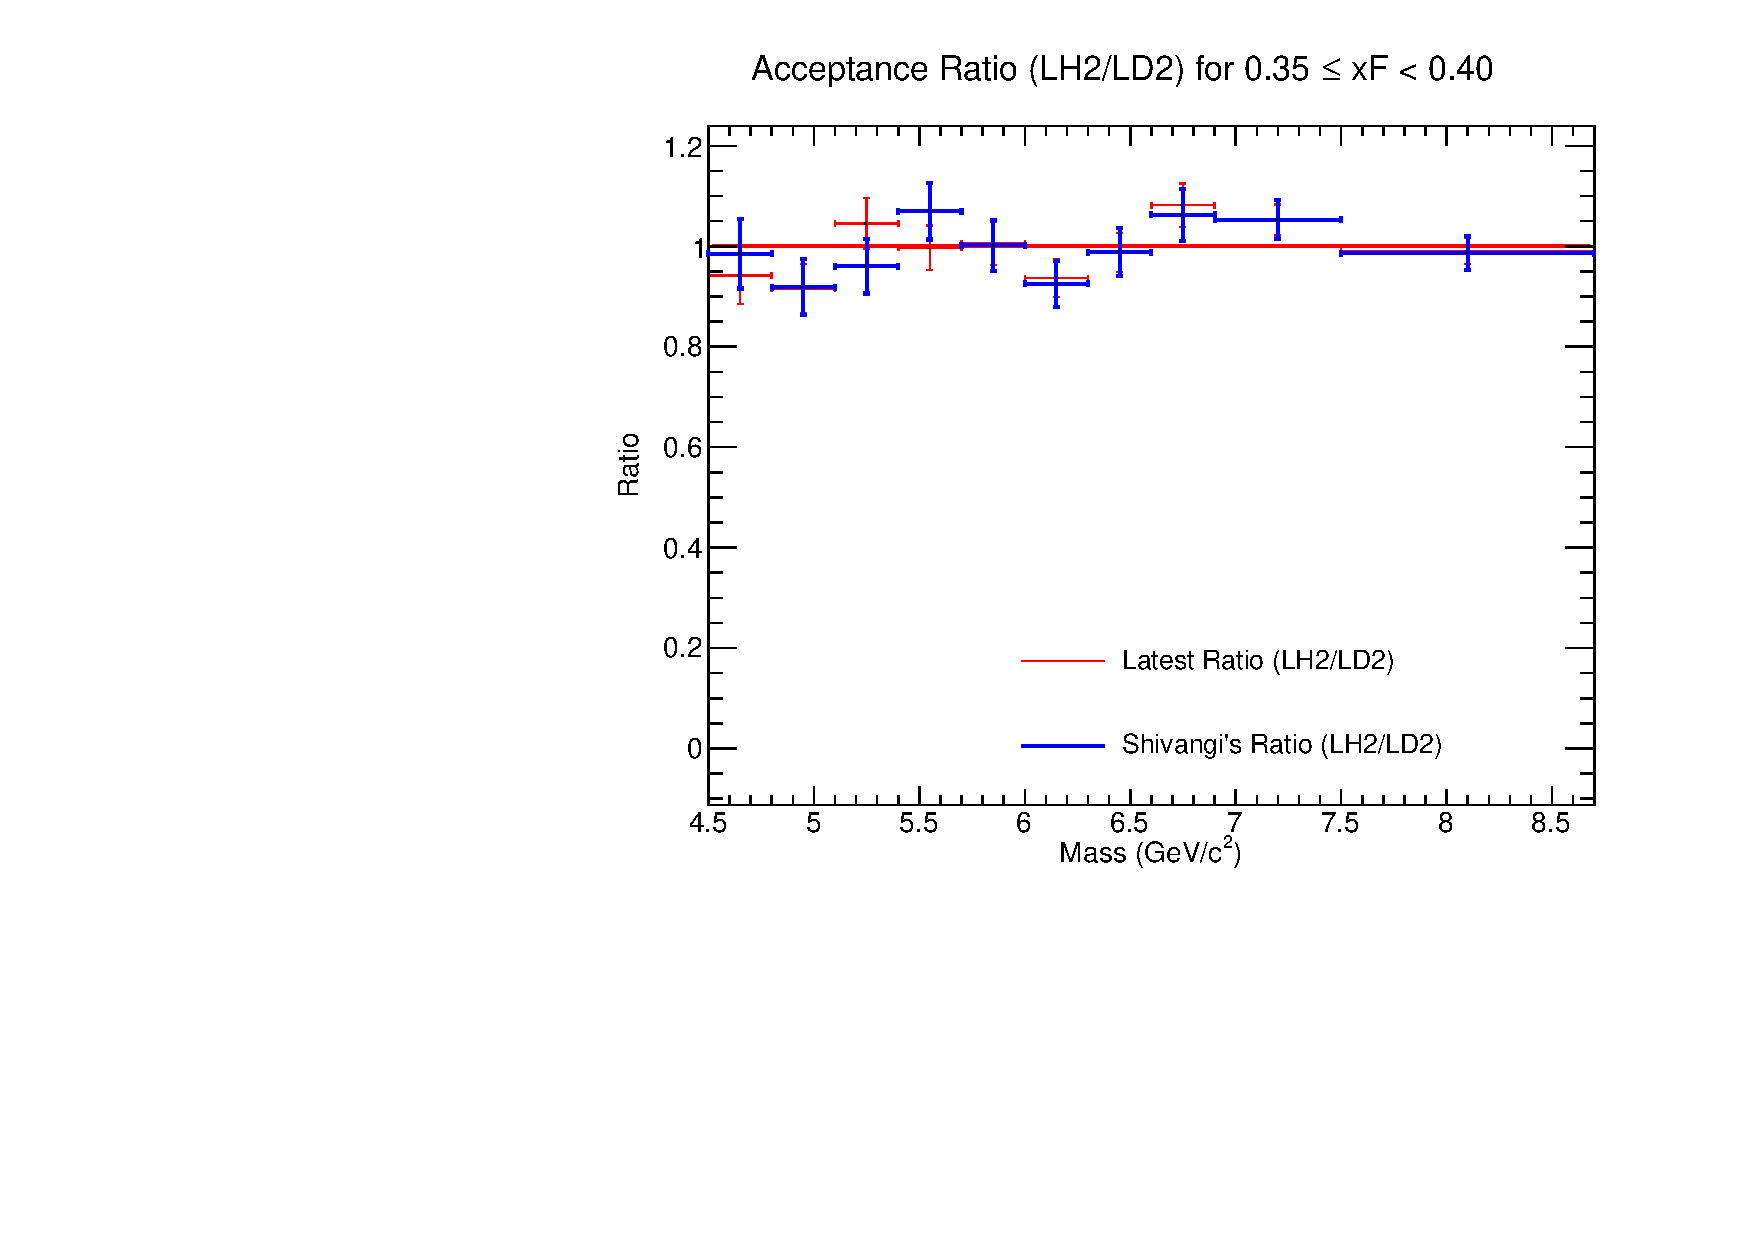
\includegraphics[width=\linewidth]{./acceptancePlots/Acceptance_ratio_xF_bin_7.pdf}
       \caption{Acceptance Ratio (LH2/LD2)}
    \end{subfigure}
    \caption{Acceptance plots for $0.35 \le x_F < 0.40$.}
\end{figure}

\begin{figure}[p]
    \centering
    \begin{subfigure}[b]{0.48\textwidth}
       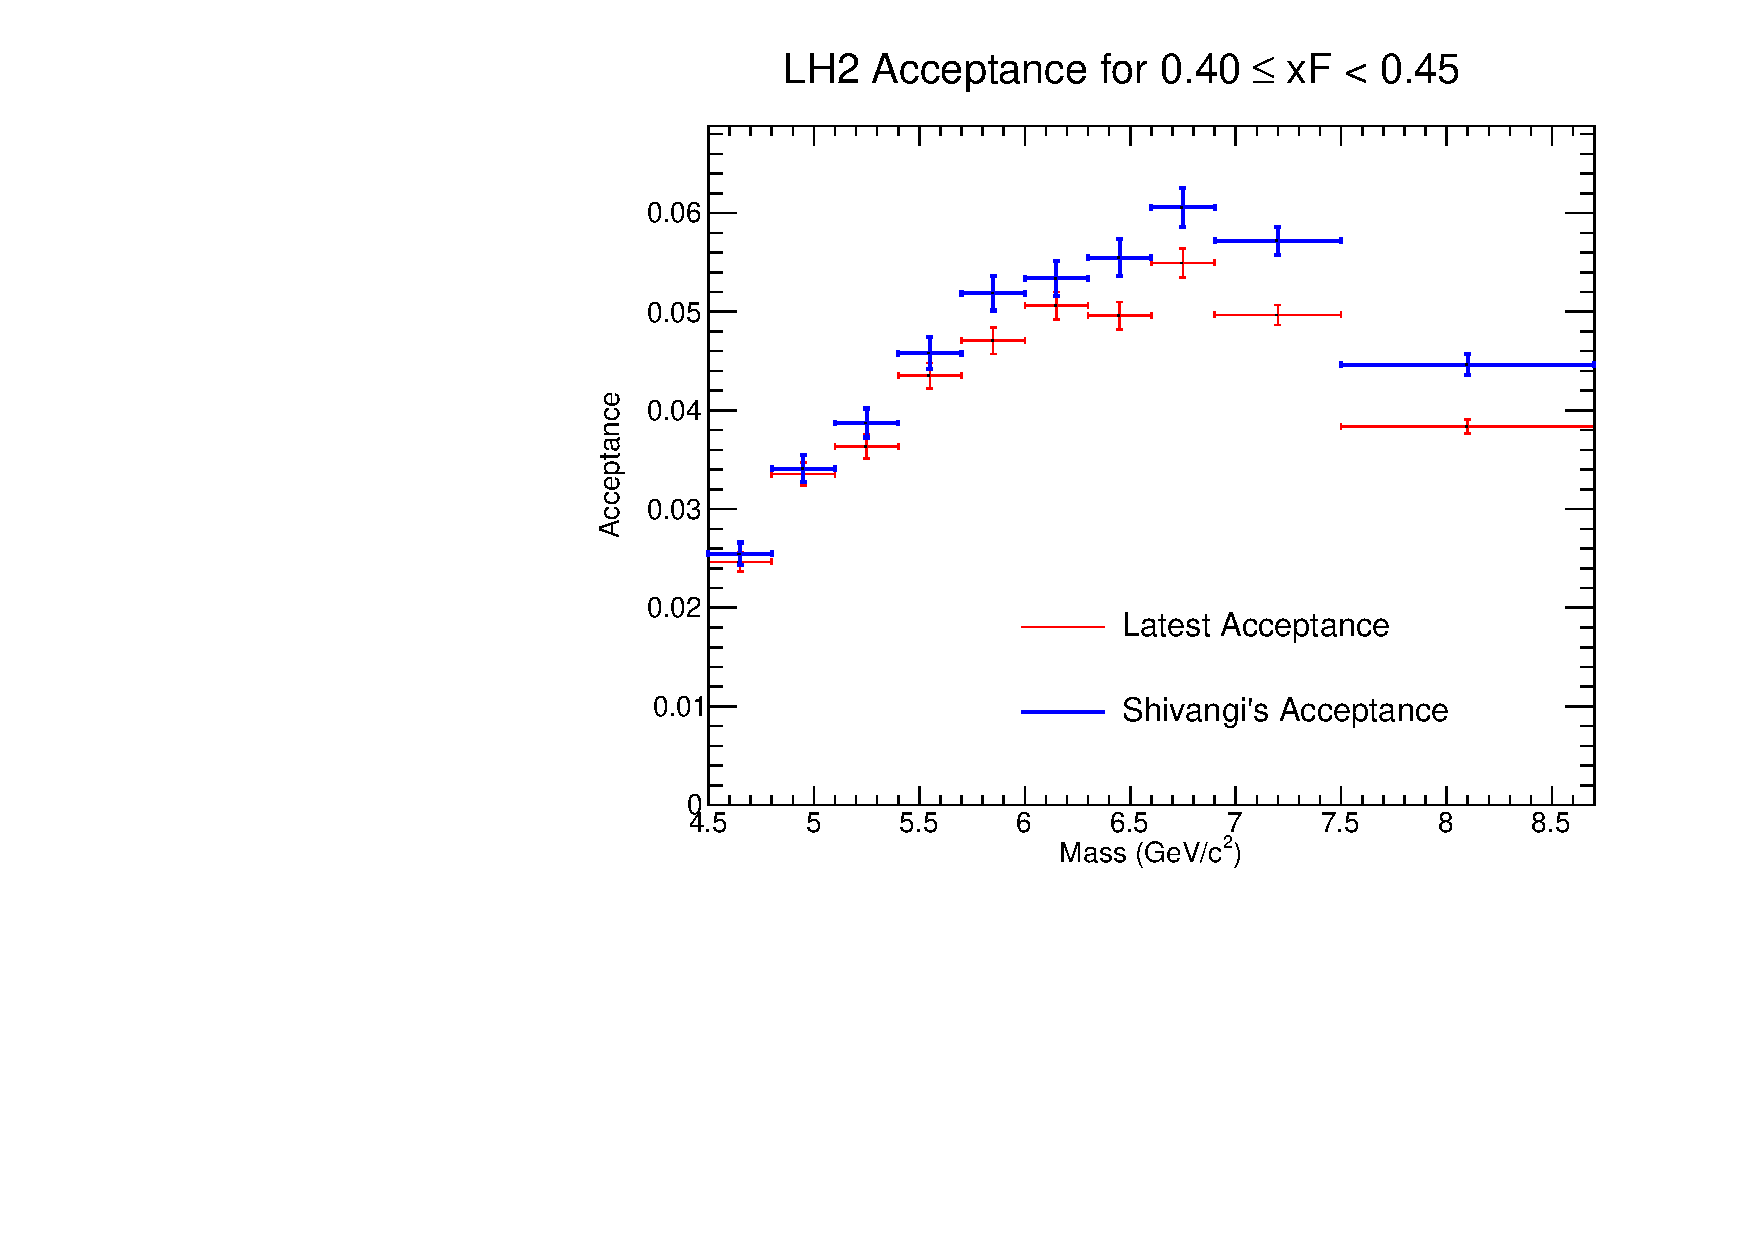
\includegraphics[width=\linewidth]{./acceptancePlots/LH2_acceptance_xF_bin_8.pdf}
       \caption{Acceptance for LH2}
    \end{subfigure}\hfill
    \begin{subfigure}[b]{0.48\textwidth}
       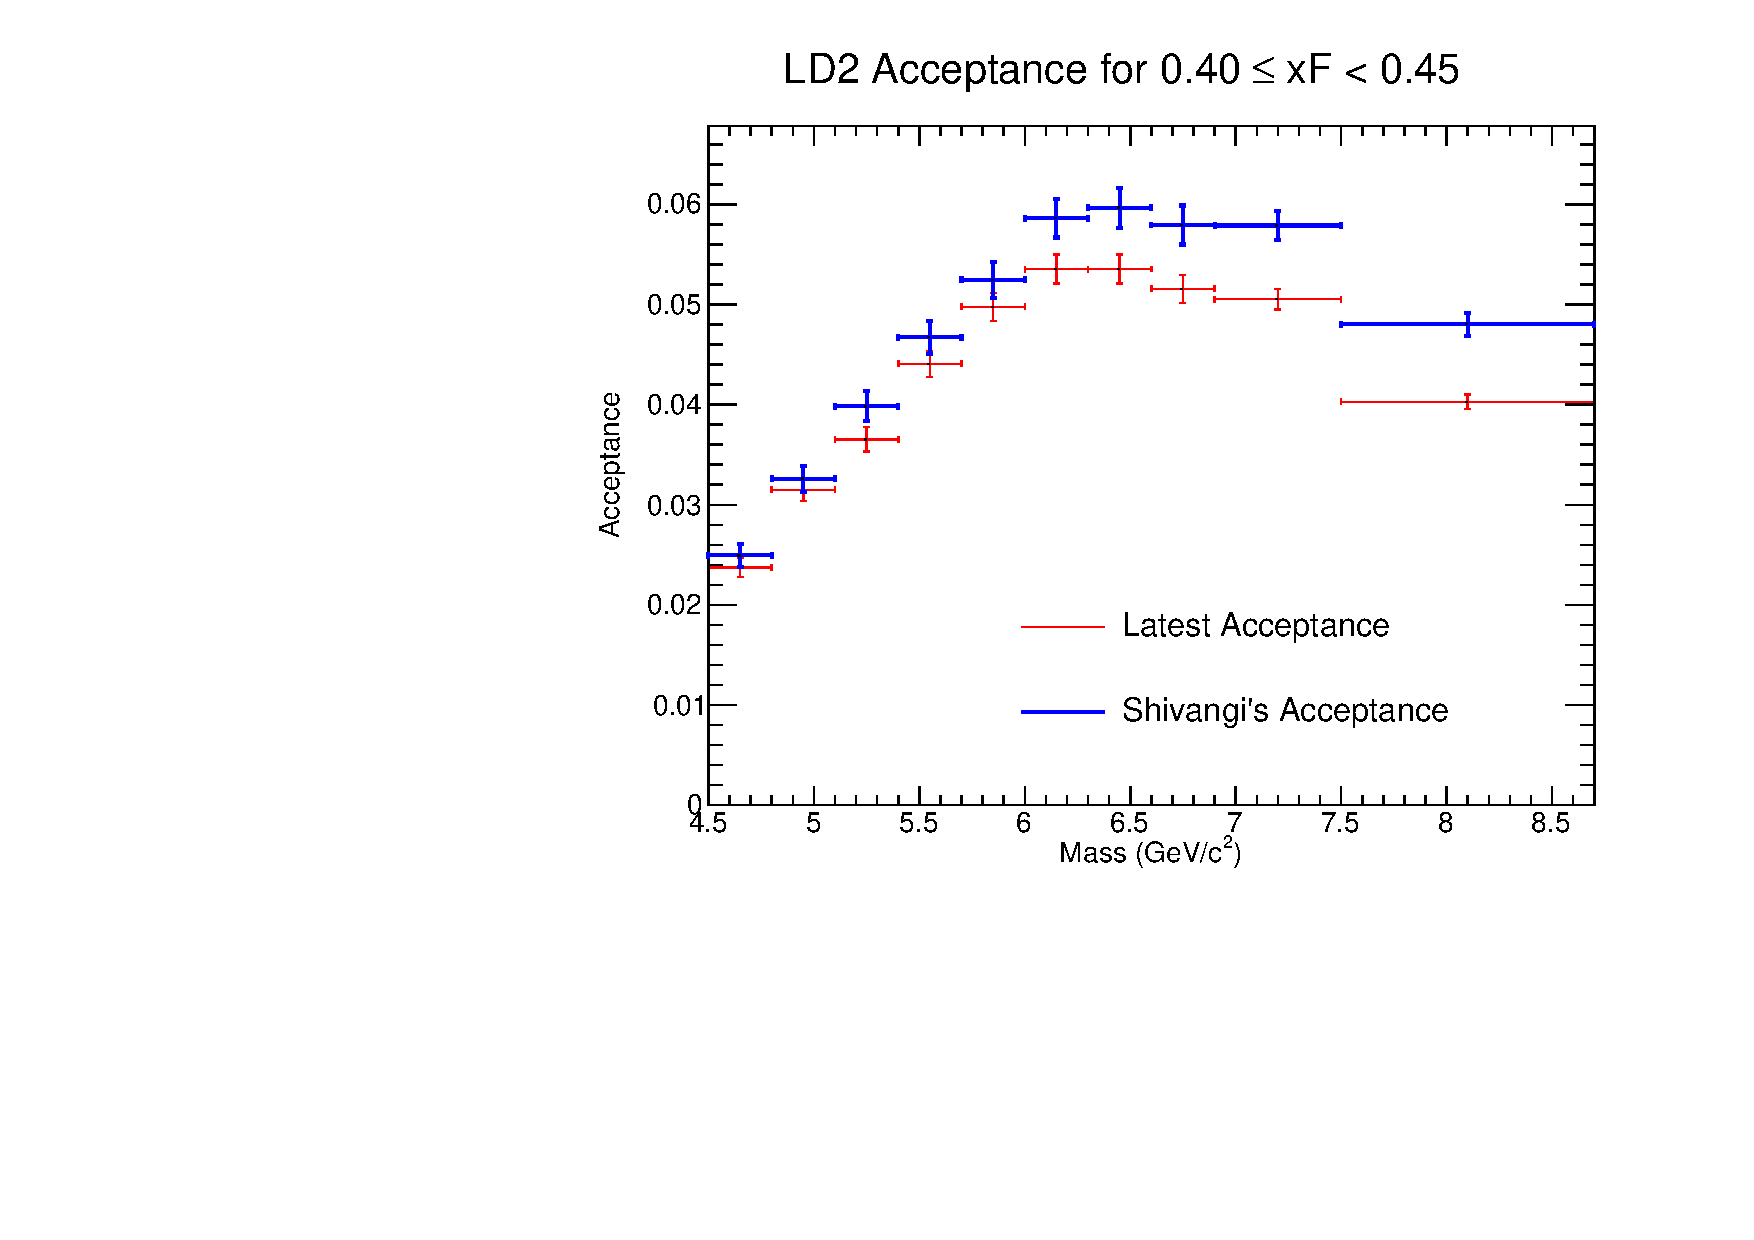
\includegraphics[width=\linewidth]{./acceptancePlots/LD2_acceptance_xF_bin_8.pdf}
       \caption{Acceptance for LD2}
    \end{subfigure}
    \begin{subfigure}[b]{0.48\textwidth}
       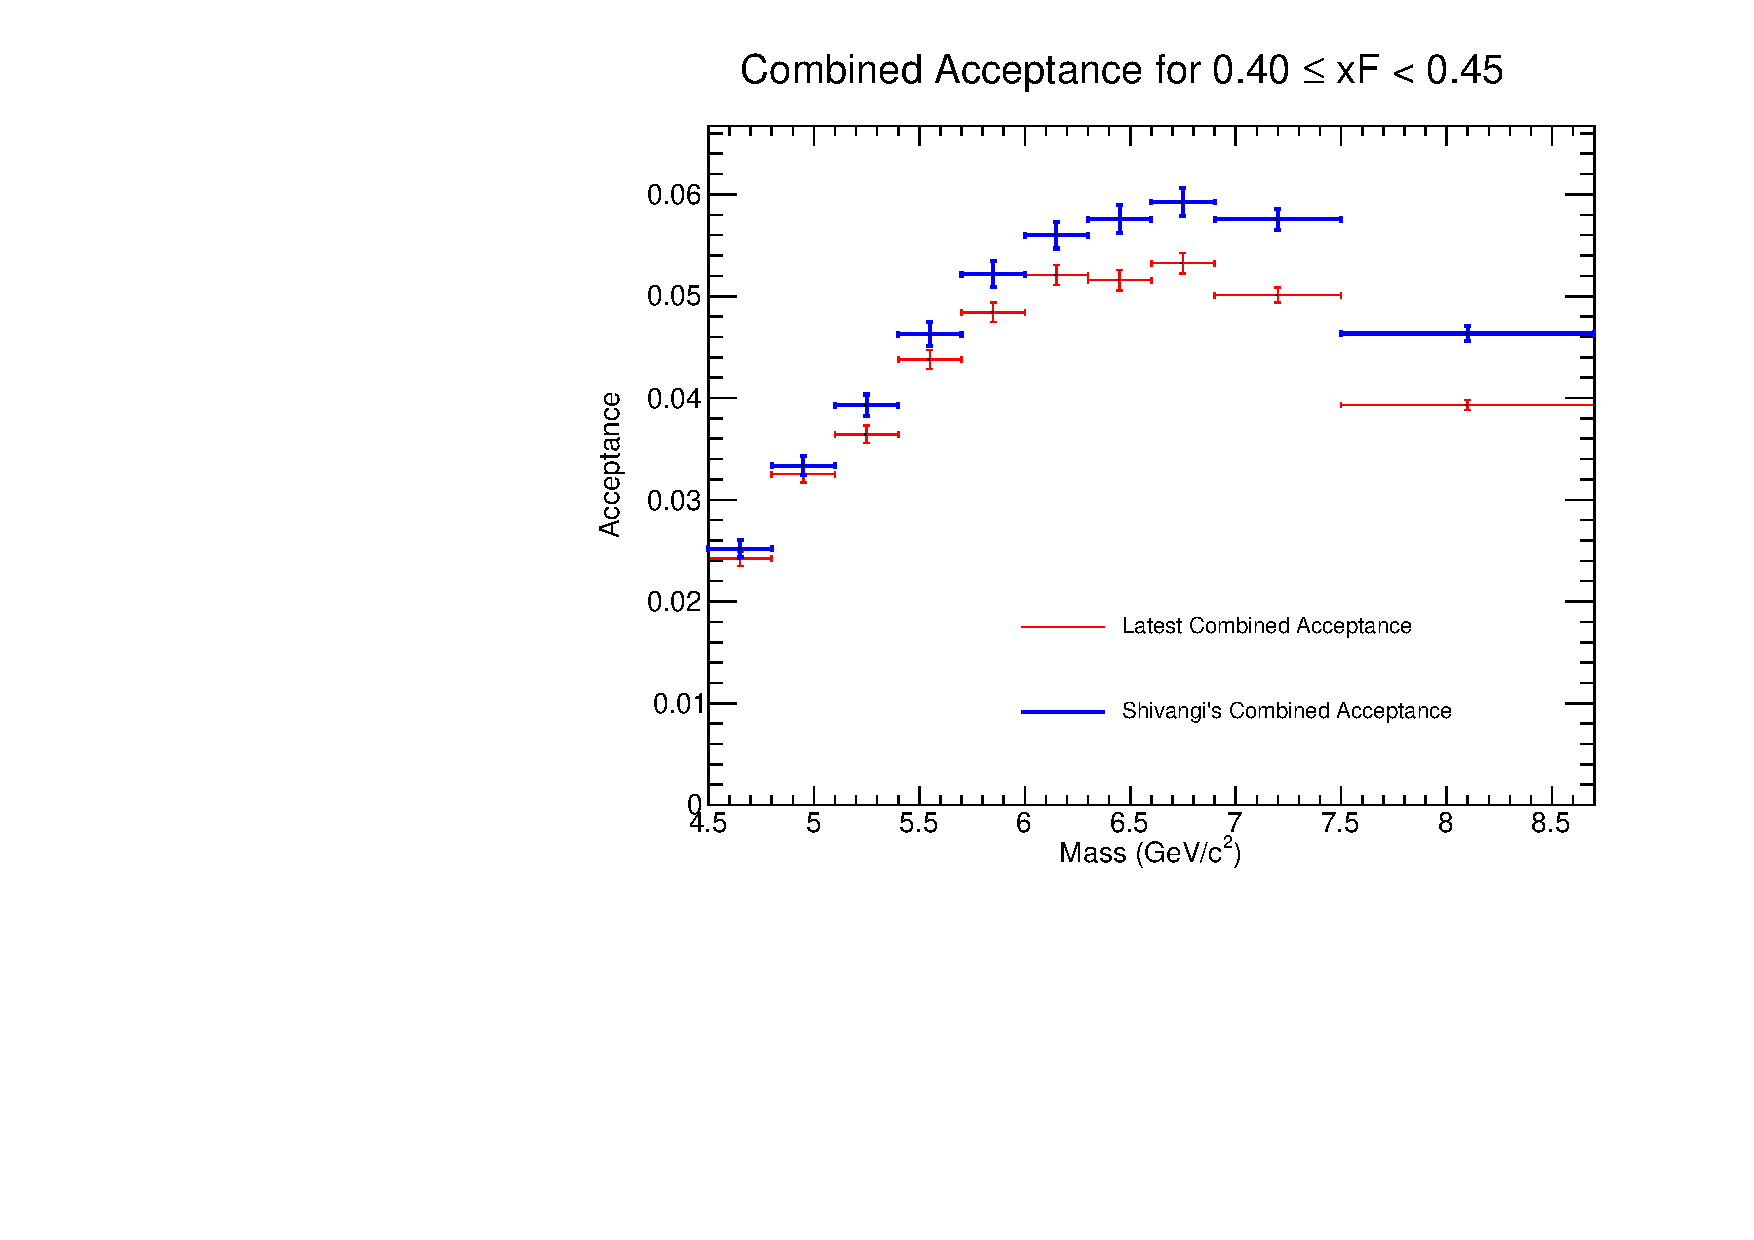
\includegraphics[width=\linewidth]{./acceptancePlots/Combined_acceptance_xF_bin_8.pdf}
       \caption{Combined Acceptance}
    \end{subfigure}\hfill
    \begin{subfigure}[b]{0.48\textwidth}
       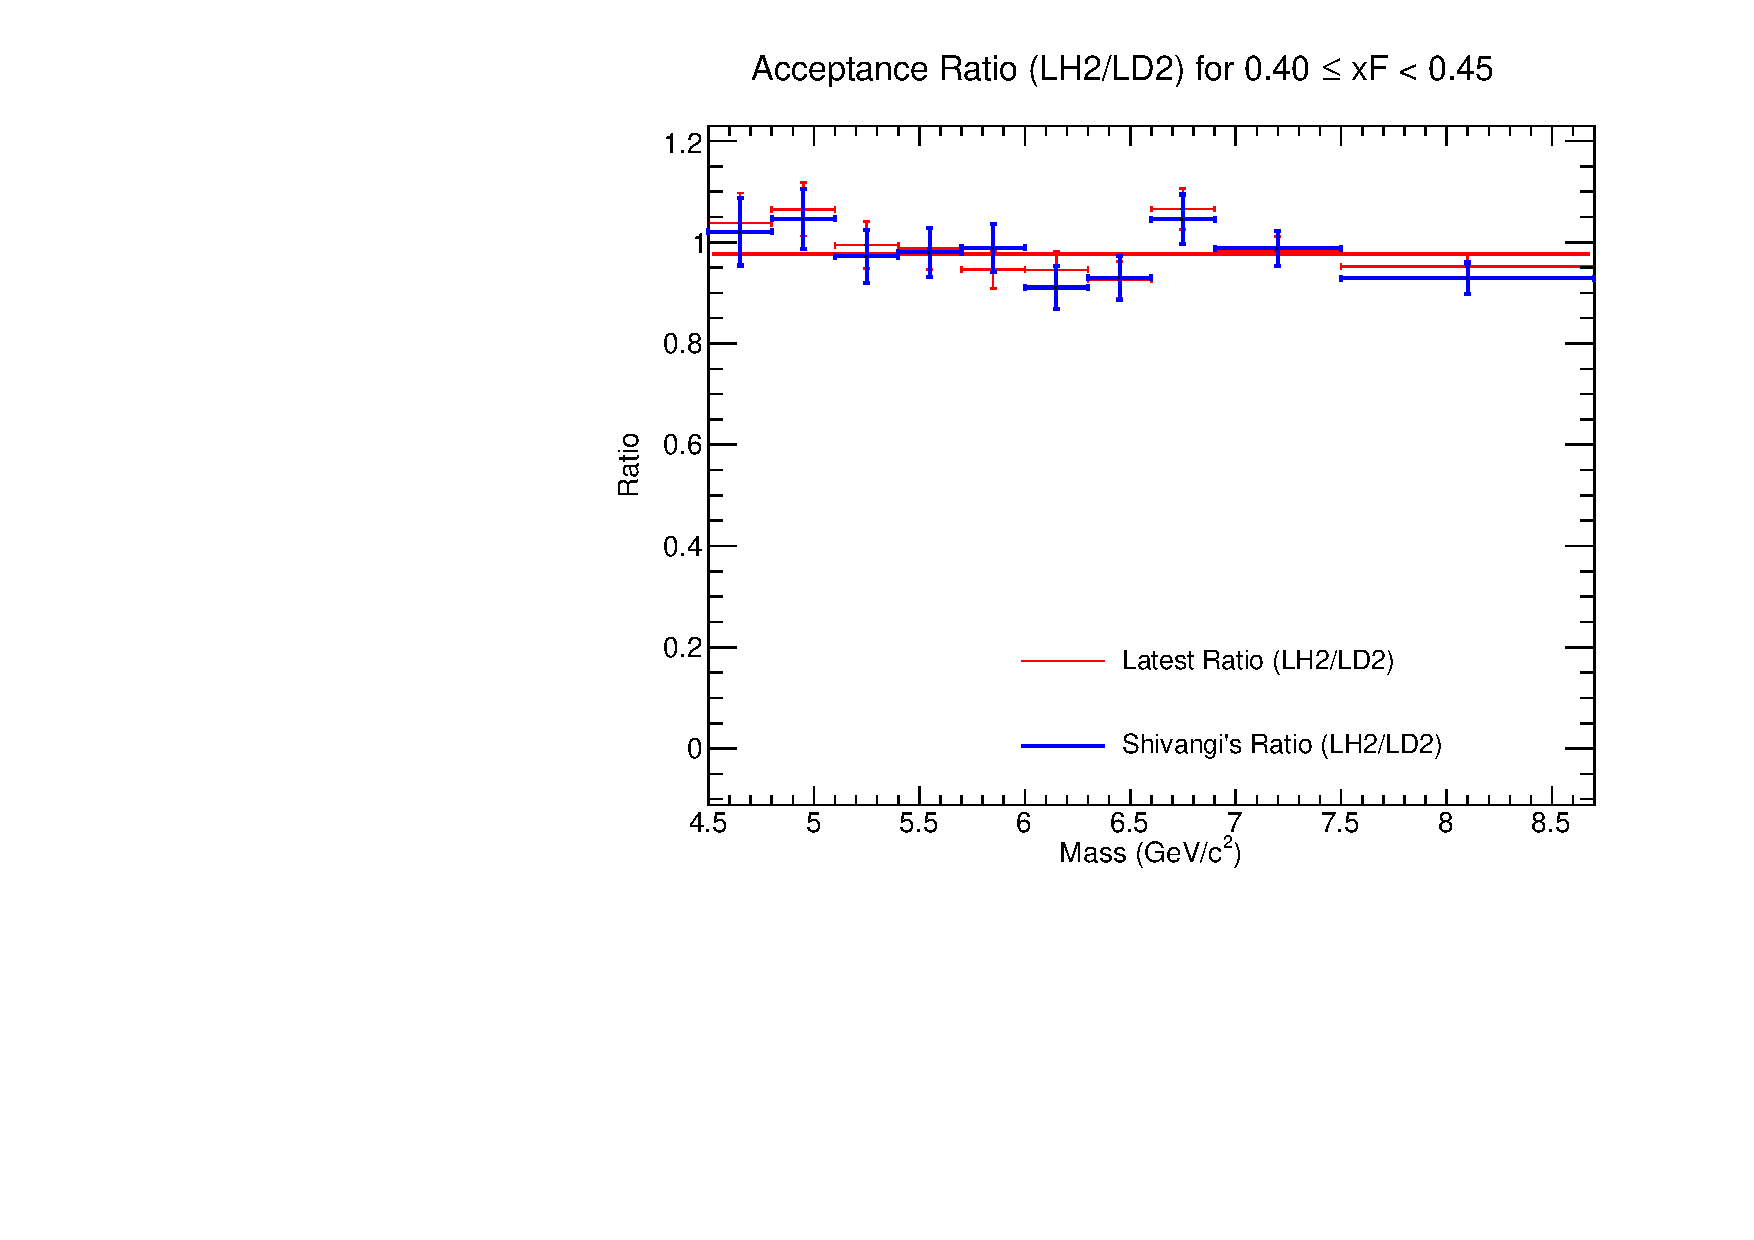
\includegraphics[width=\linewidth]{./acceptancePlots/Acceptance_ratio_xF_bin_8.pdf}
       \caption{Acceptance Ratio (LH2/LD2)}
    \end{subfigure}
    \caption{Acceptance plots for $0.40 \le x_F < 0.45$.}
\end{figure}

\begin{figure}[p]
    \centering
    \begin{subfigure}[b]{0.48\textwidth}
       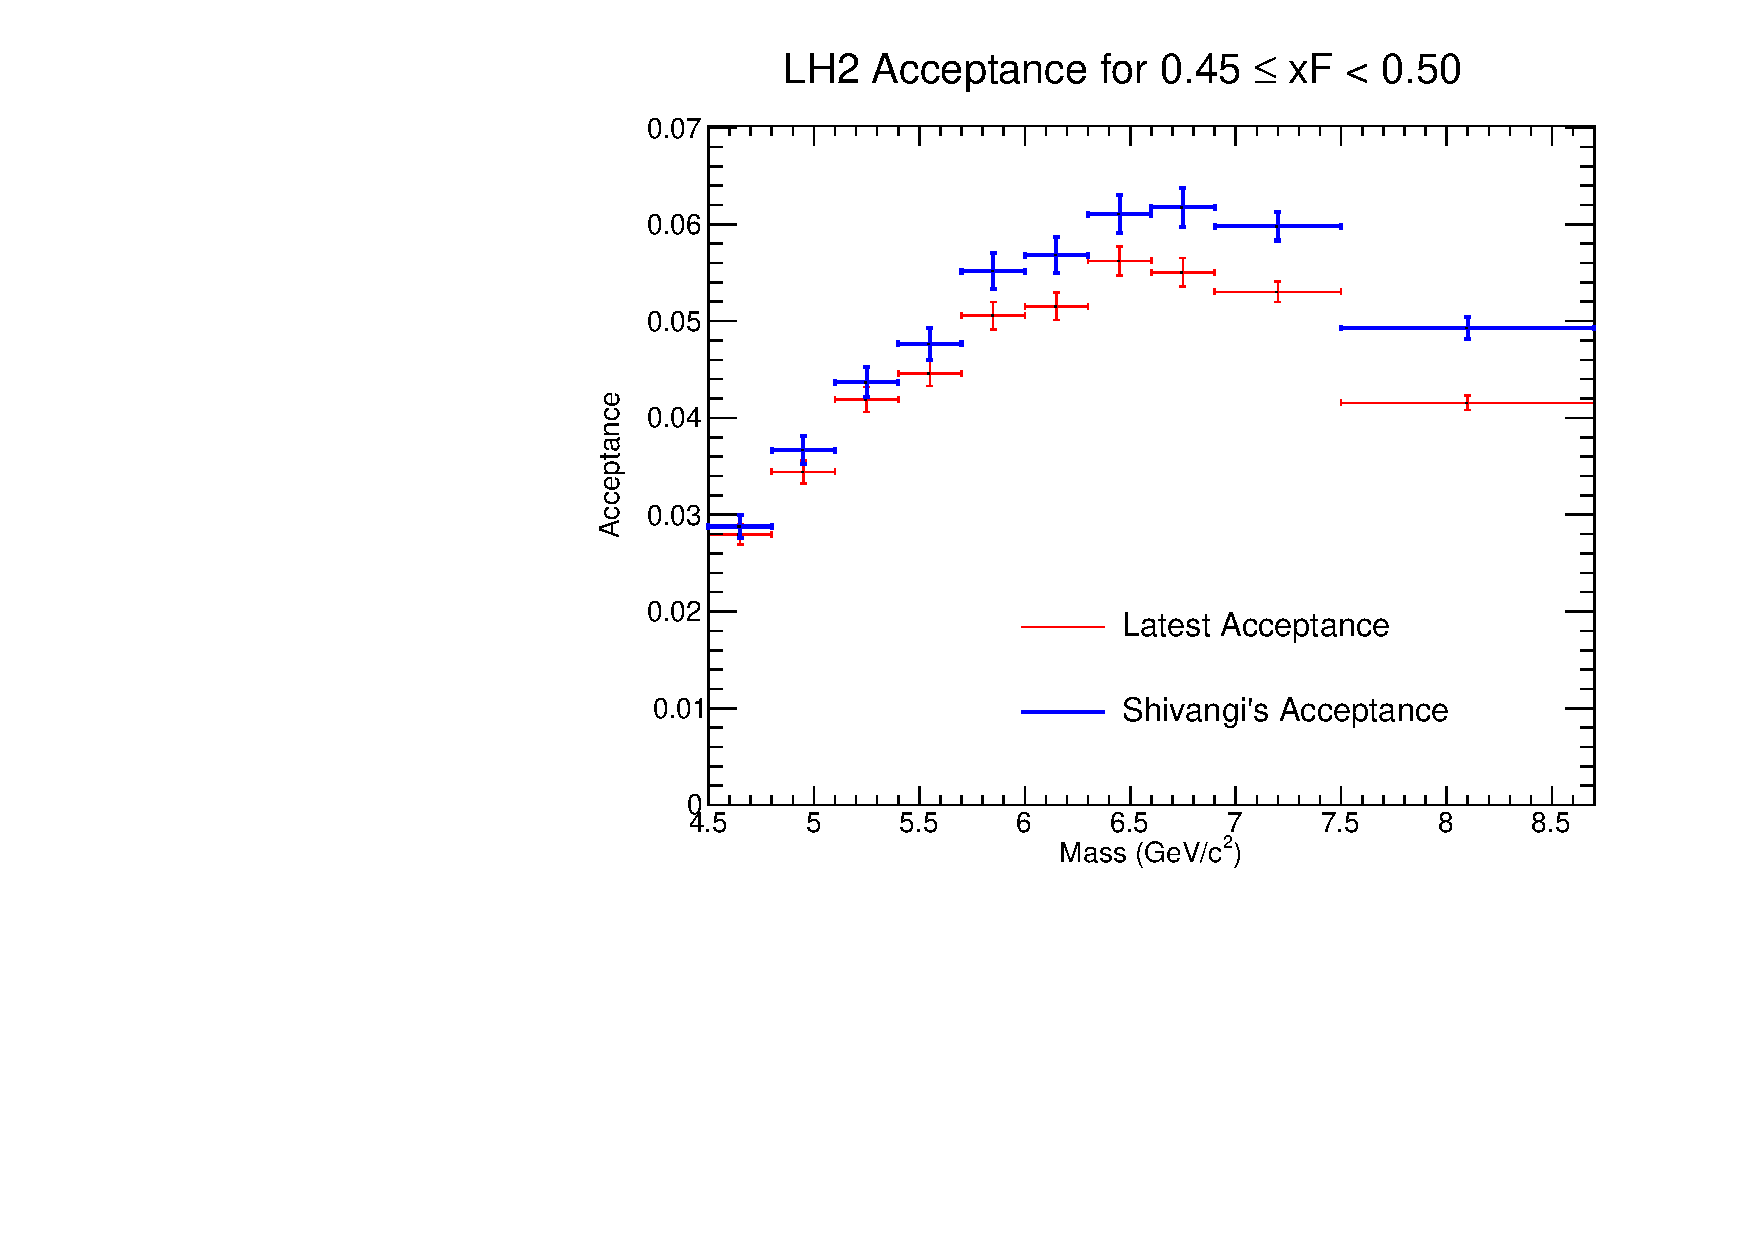
\includegraphics[width=\linewidth]{./acceptancePlots/LH2_acceptance_xF_bin_9.pdf}
       \caption{Acceptance for LH2}
    \end{subfigure}\hfill
    \begin{subfigure}[b]{0.48\textwidth}
       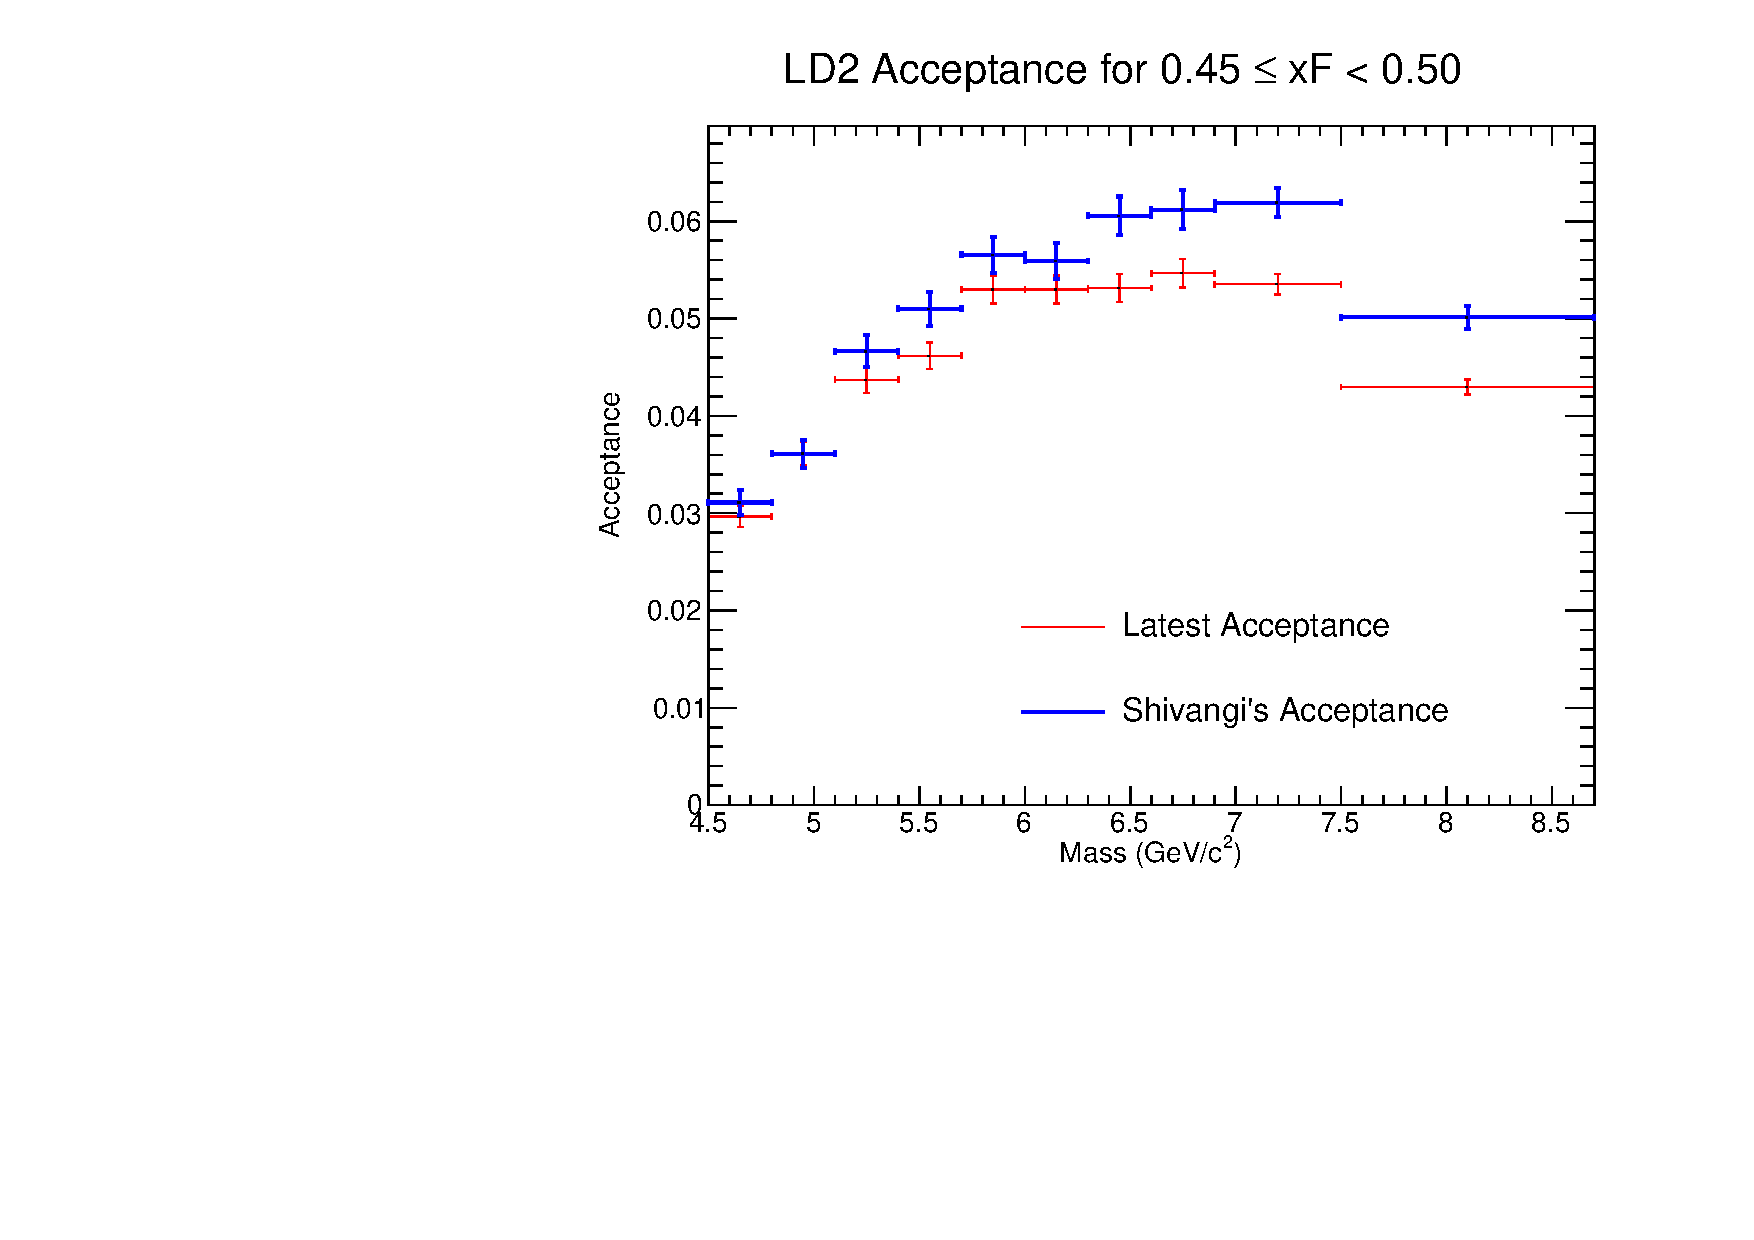
\includegraphics[width=\linewidth]{./acceptancePlots/LD2_acceptance_xF_bin_9.pdf}
       \caption{Acceptance for LD2}
    \end{subfigure}
    \begin{subfigure}[b]{0.48\textwidth}
       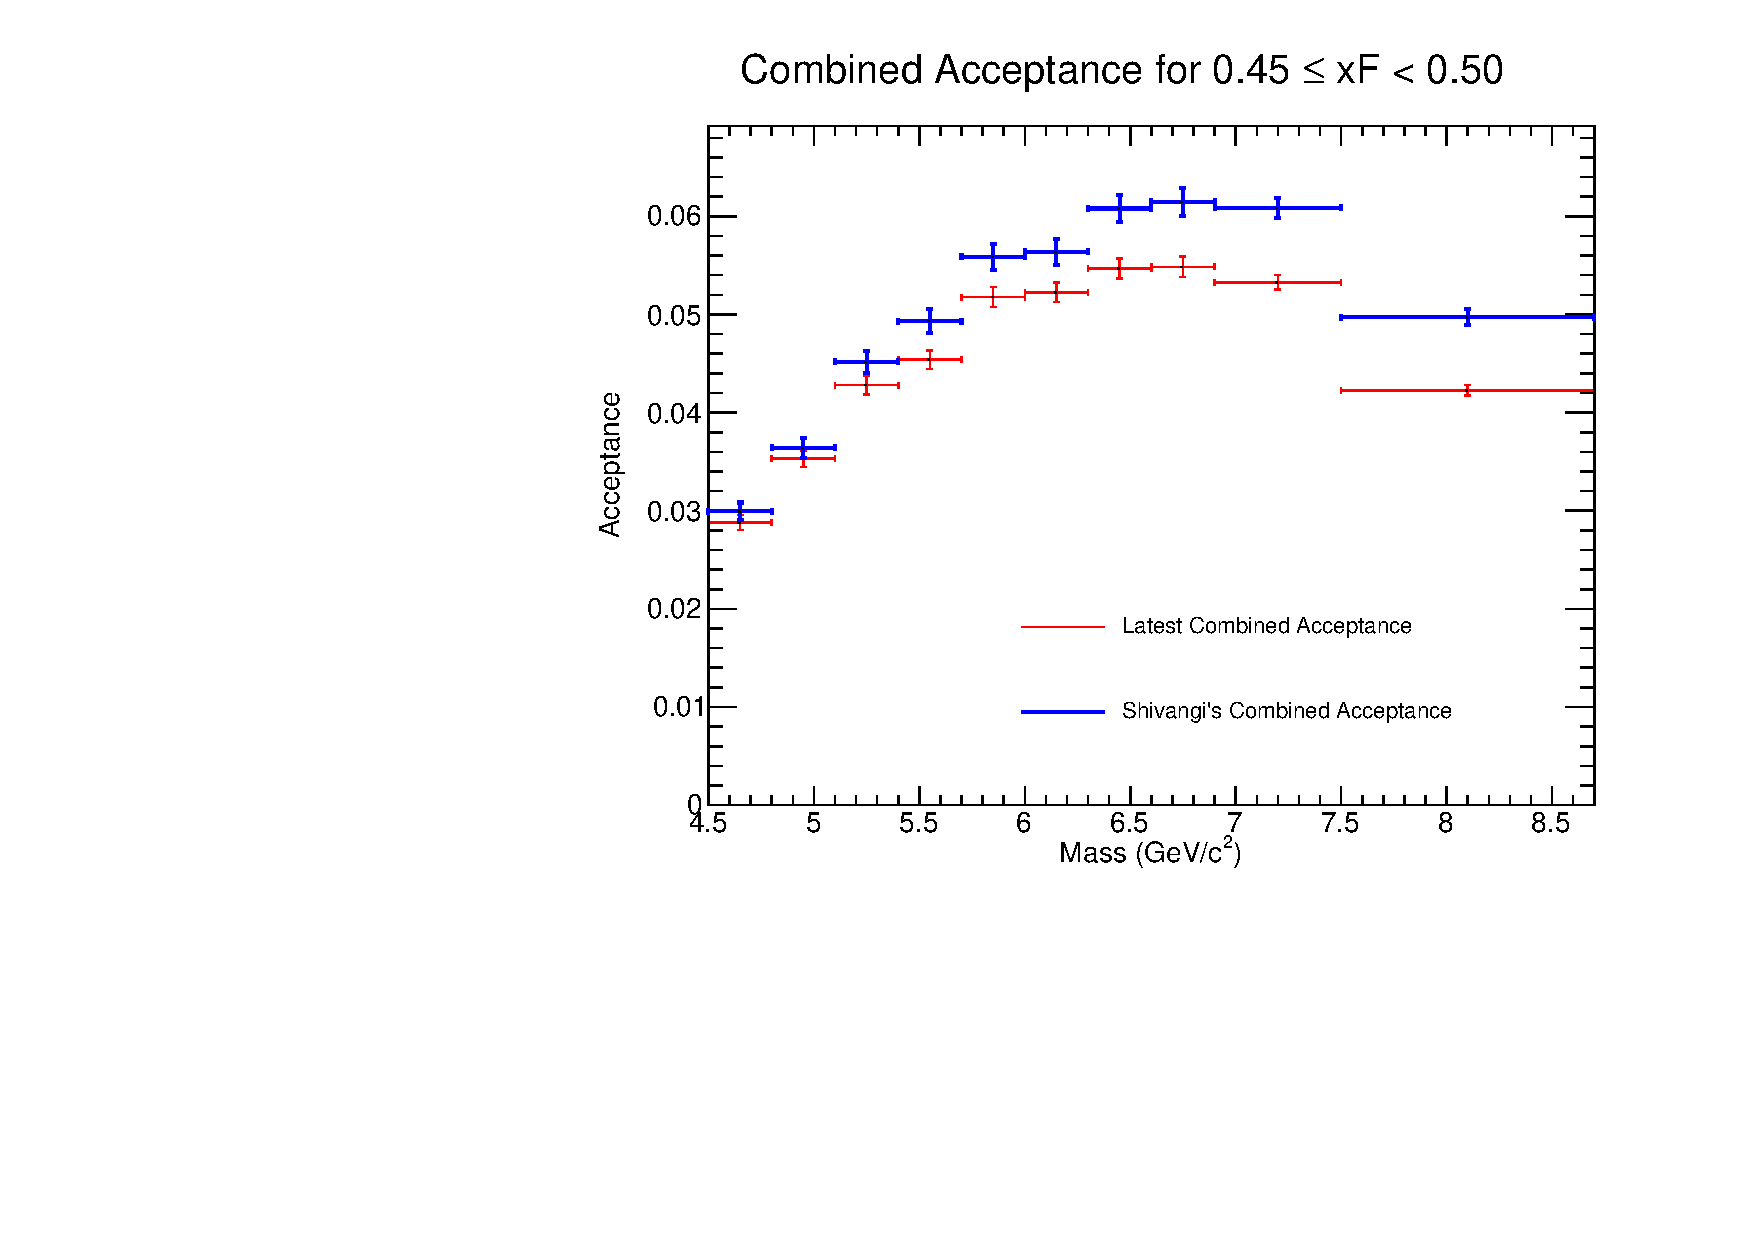
\includegraphics[width=\linewidth]{./acceptancePlots/Combined_acceptance_xF_bin_9.pdf}
       \caption{Combined Acceptance}
    \end{subfigure}\hfill
    \begin{subfigure}[b]{0.48\textwidth}
       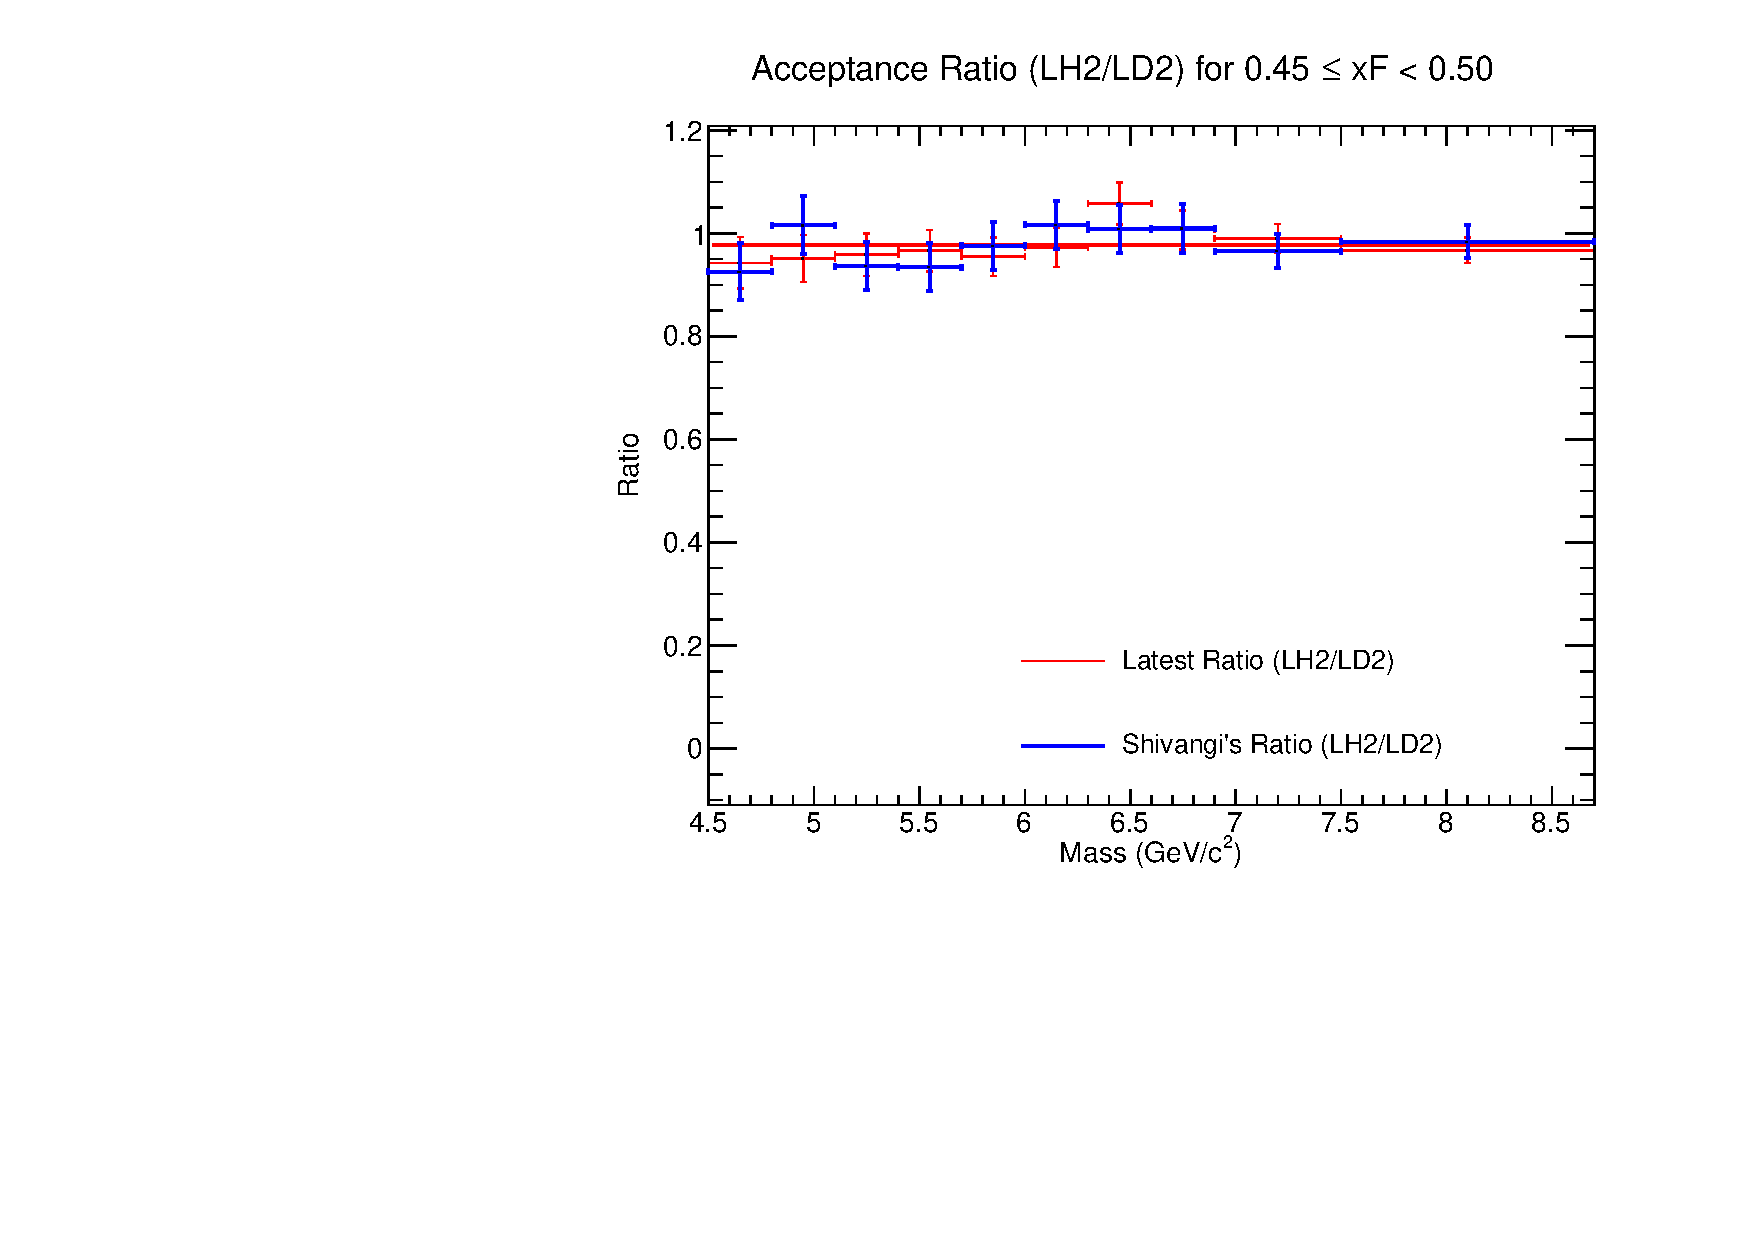
\includegraphics[width=\linewidth]{./acceptancePlots/Acceptance_ratio_xF_bin_9.pdf}
       \caption{Acceptance Ratio (LH2/LD2)}
    \end{subfigure}
    \caption{Acceptance plots for $0.45 \le x_F < 0.50$.}
\end{figure}

\begin{figure}[p]
    \centering
    \begin{subfigure}[b]{0.48\textwidth}
       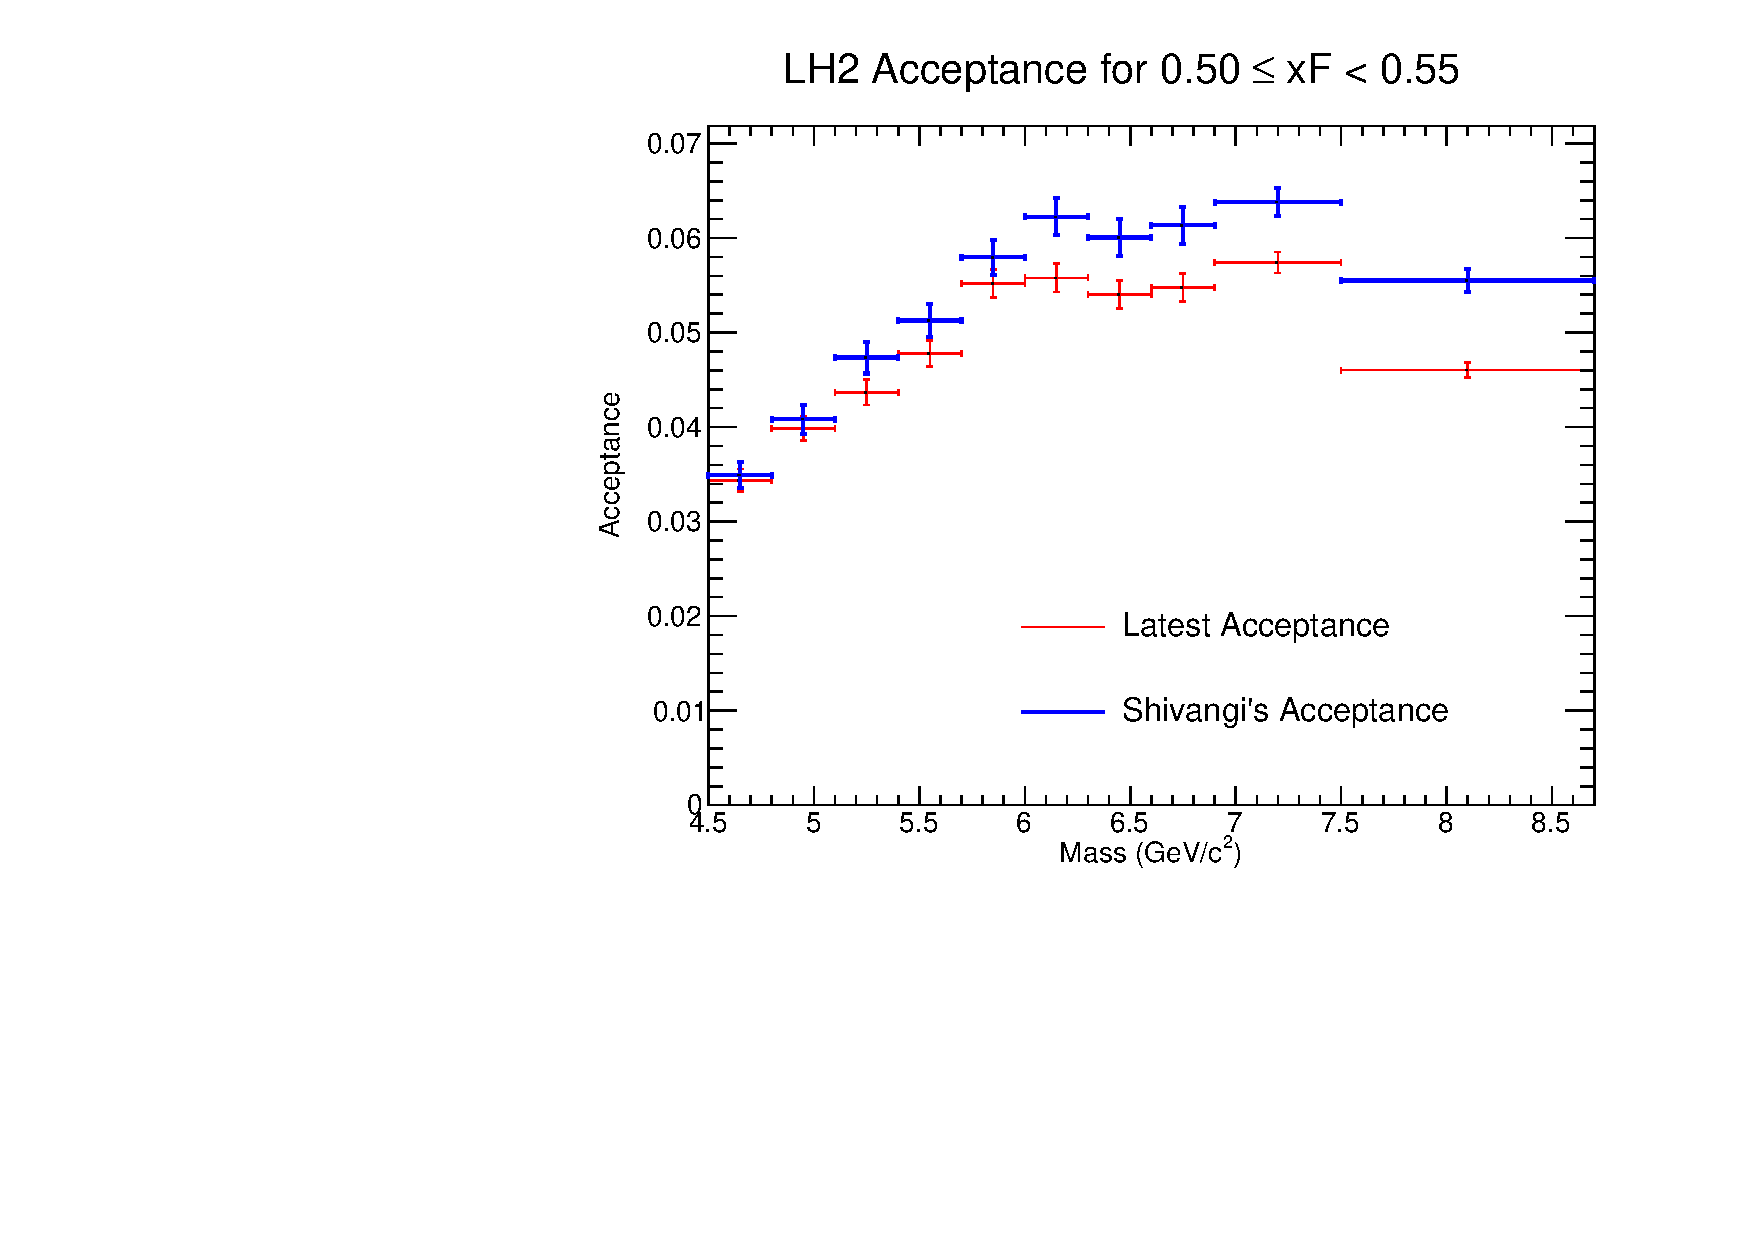
\includegraphics[width=\linewidth]{./acceptancePlots/LH2_acceptance_xF_bin_10.pdf}
       \caption{Acceptance for LH2}
    \end{subfigure}\hfill
    \begin{subfigure}[b]{0.48\textwidth}
       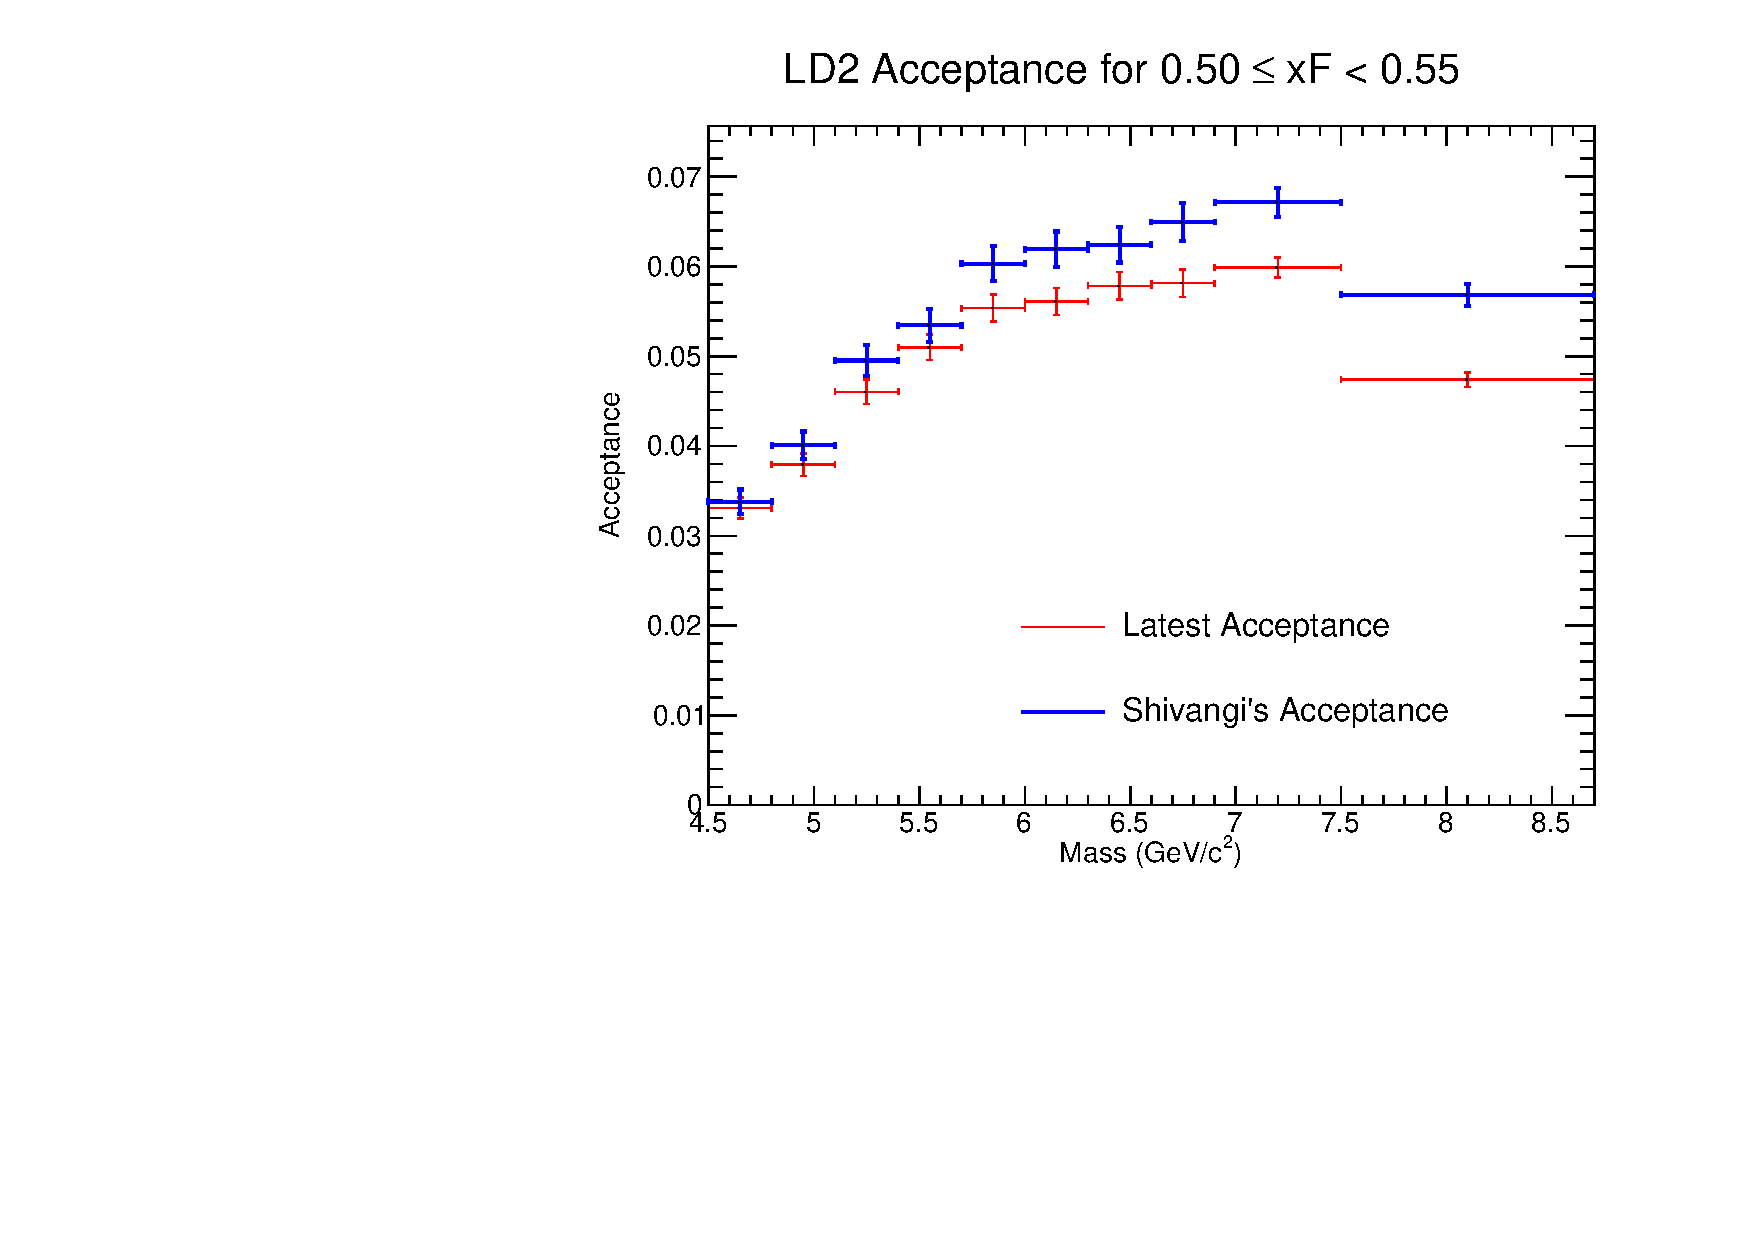
\includegraphics[width=\linewidth]{./acceptancePlots/LD2_acceptance_xF_bin_10.pdf}
       \caption{Acceptance for LD2}
    \end{subfigure}
    \begin{subfigure}[b]{0.48\textwidth}
       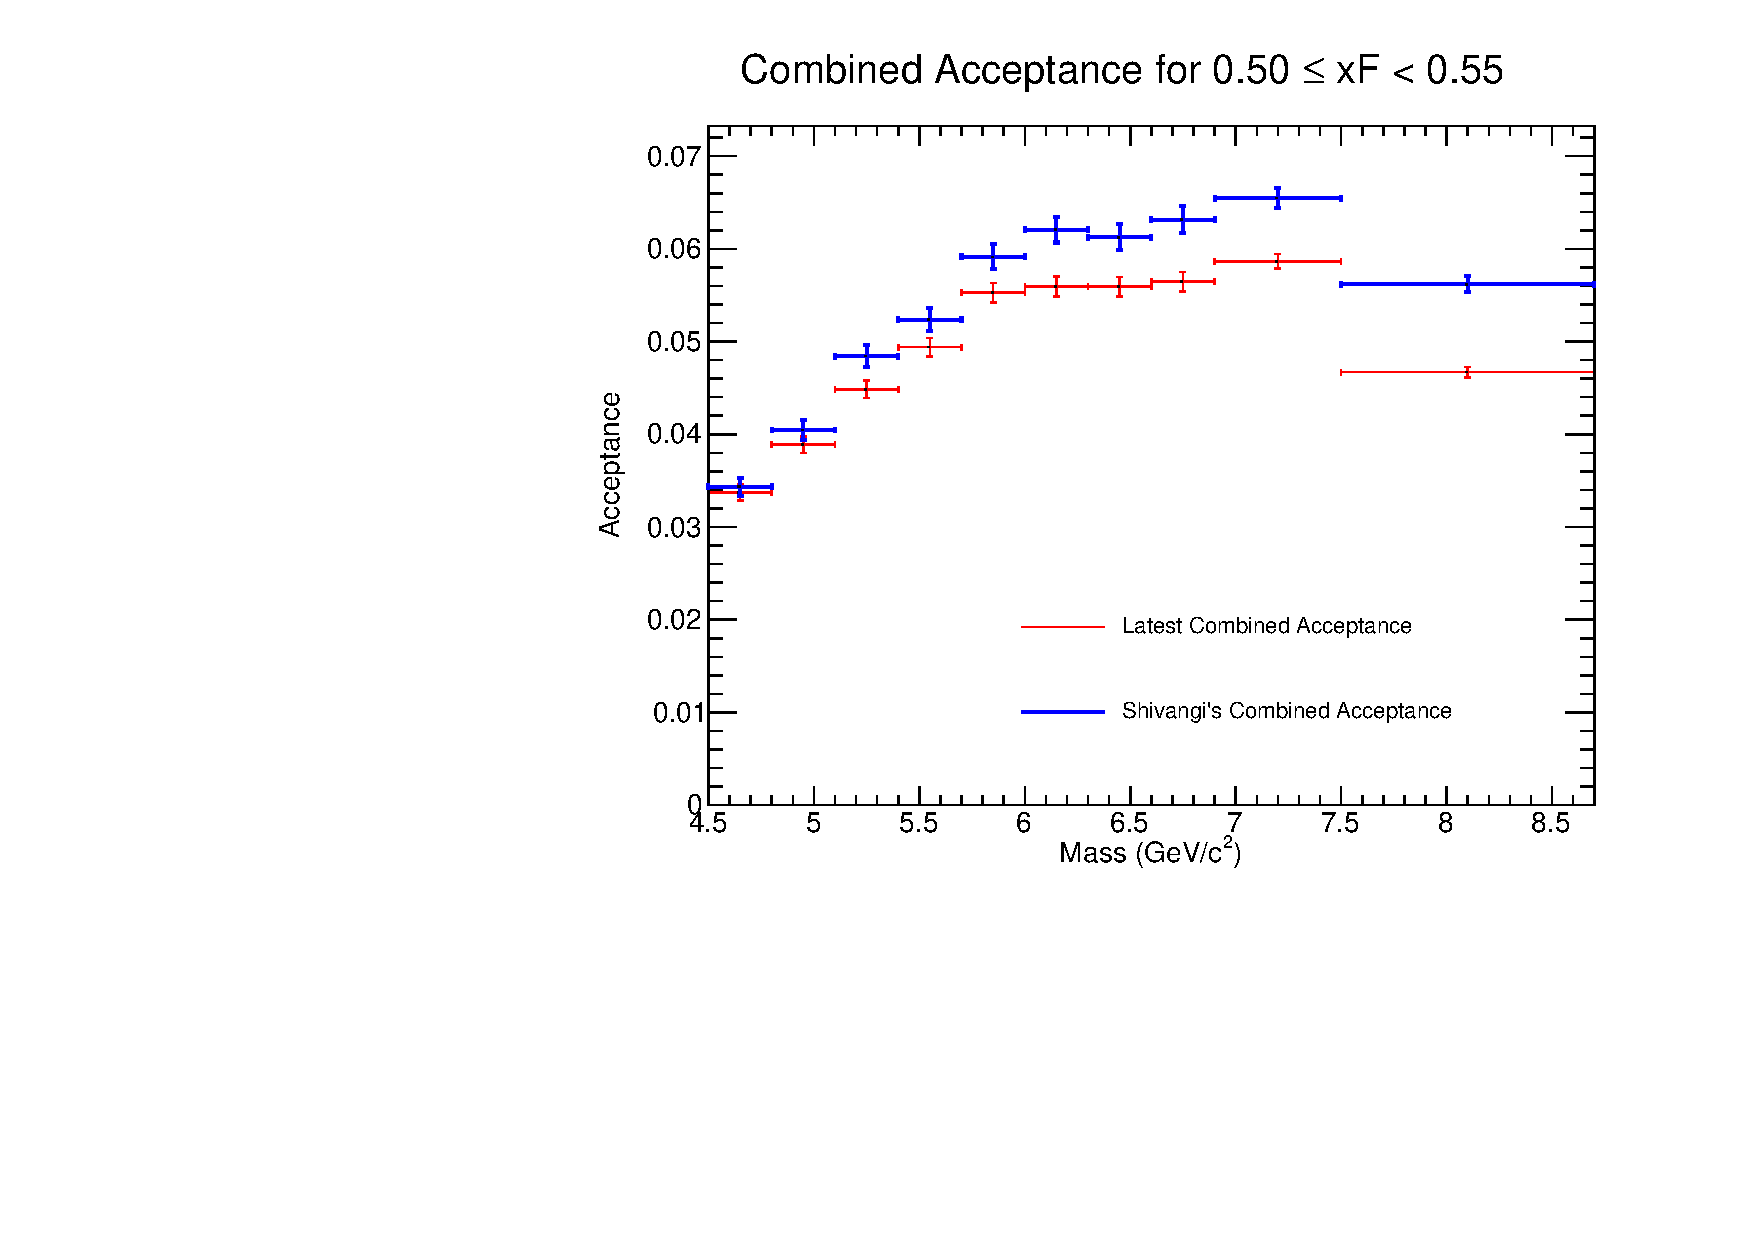
\includegraphics[width=\linewidth]{./acceptancePlots/Combined_acceptance_xF_bin_10.pdf}
       \caption{Combined Acceptance}
    \end{subfigure}\hfill
    \begin{subfigure}[b]{0.48\textwidth}
       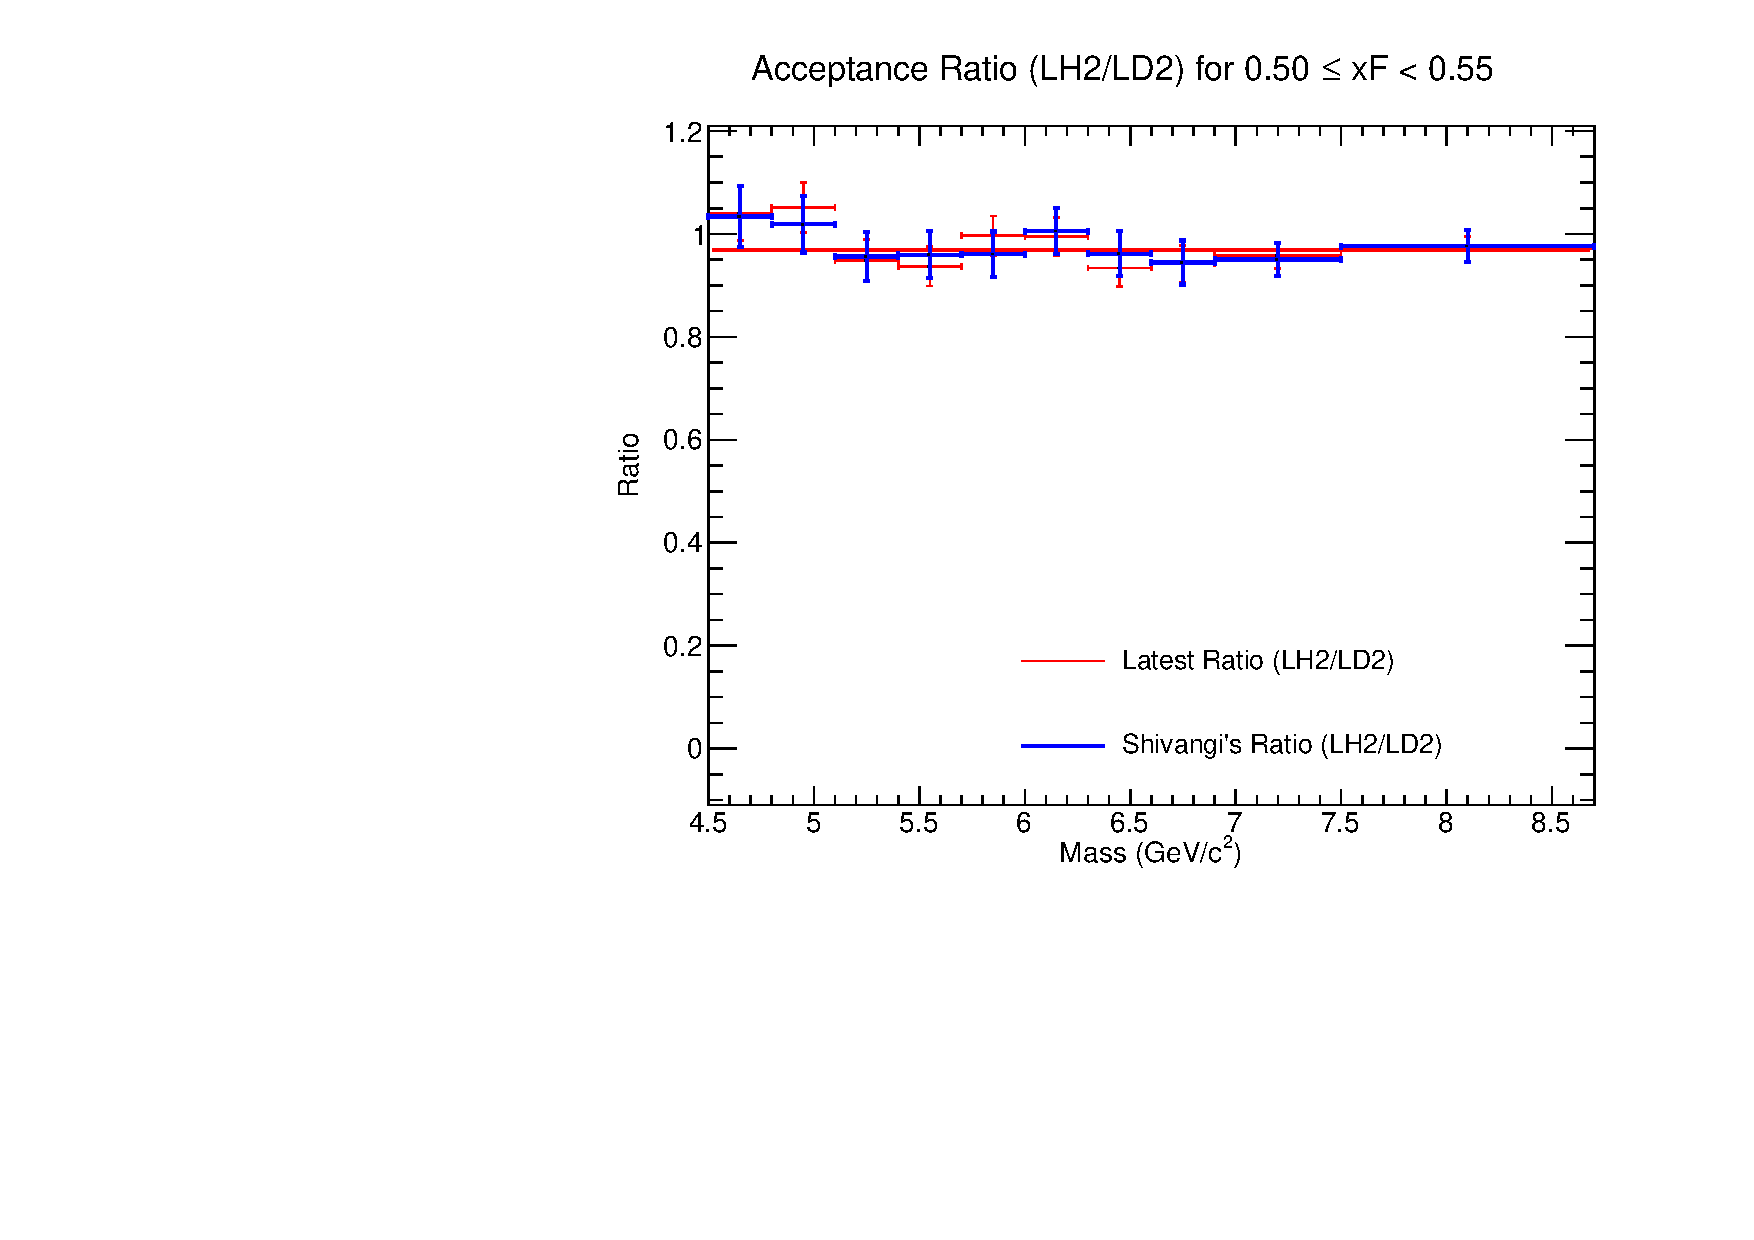
\includegraphics[width=\linewidth]{./acceptancePlots/Acceptance_ratio_xF_bin_10.pdf}
       \caption{Acceptance Ratio (LH2/LD2)}
    \end{subfigure}
    \caption{Acceptance plots for $0.50 \le x_F < 0.55$.}
\end{figure}

\begin{figure}[p]
    \centering
    \begin{subfigure}[b]{0.48\textwidth}
       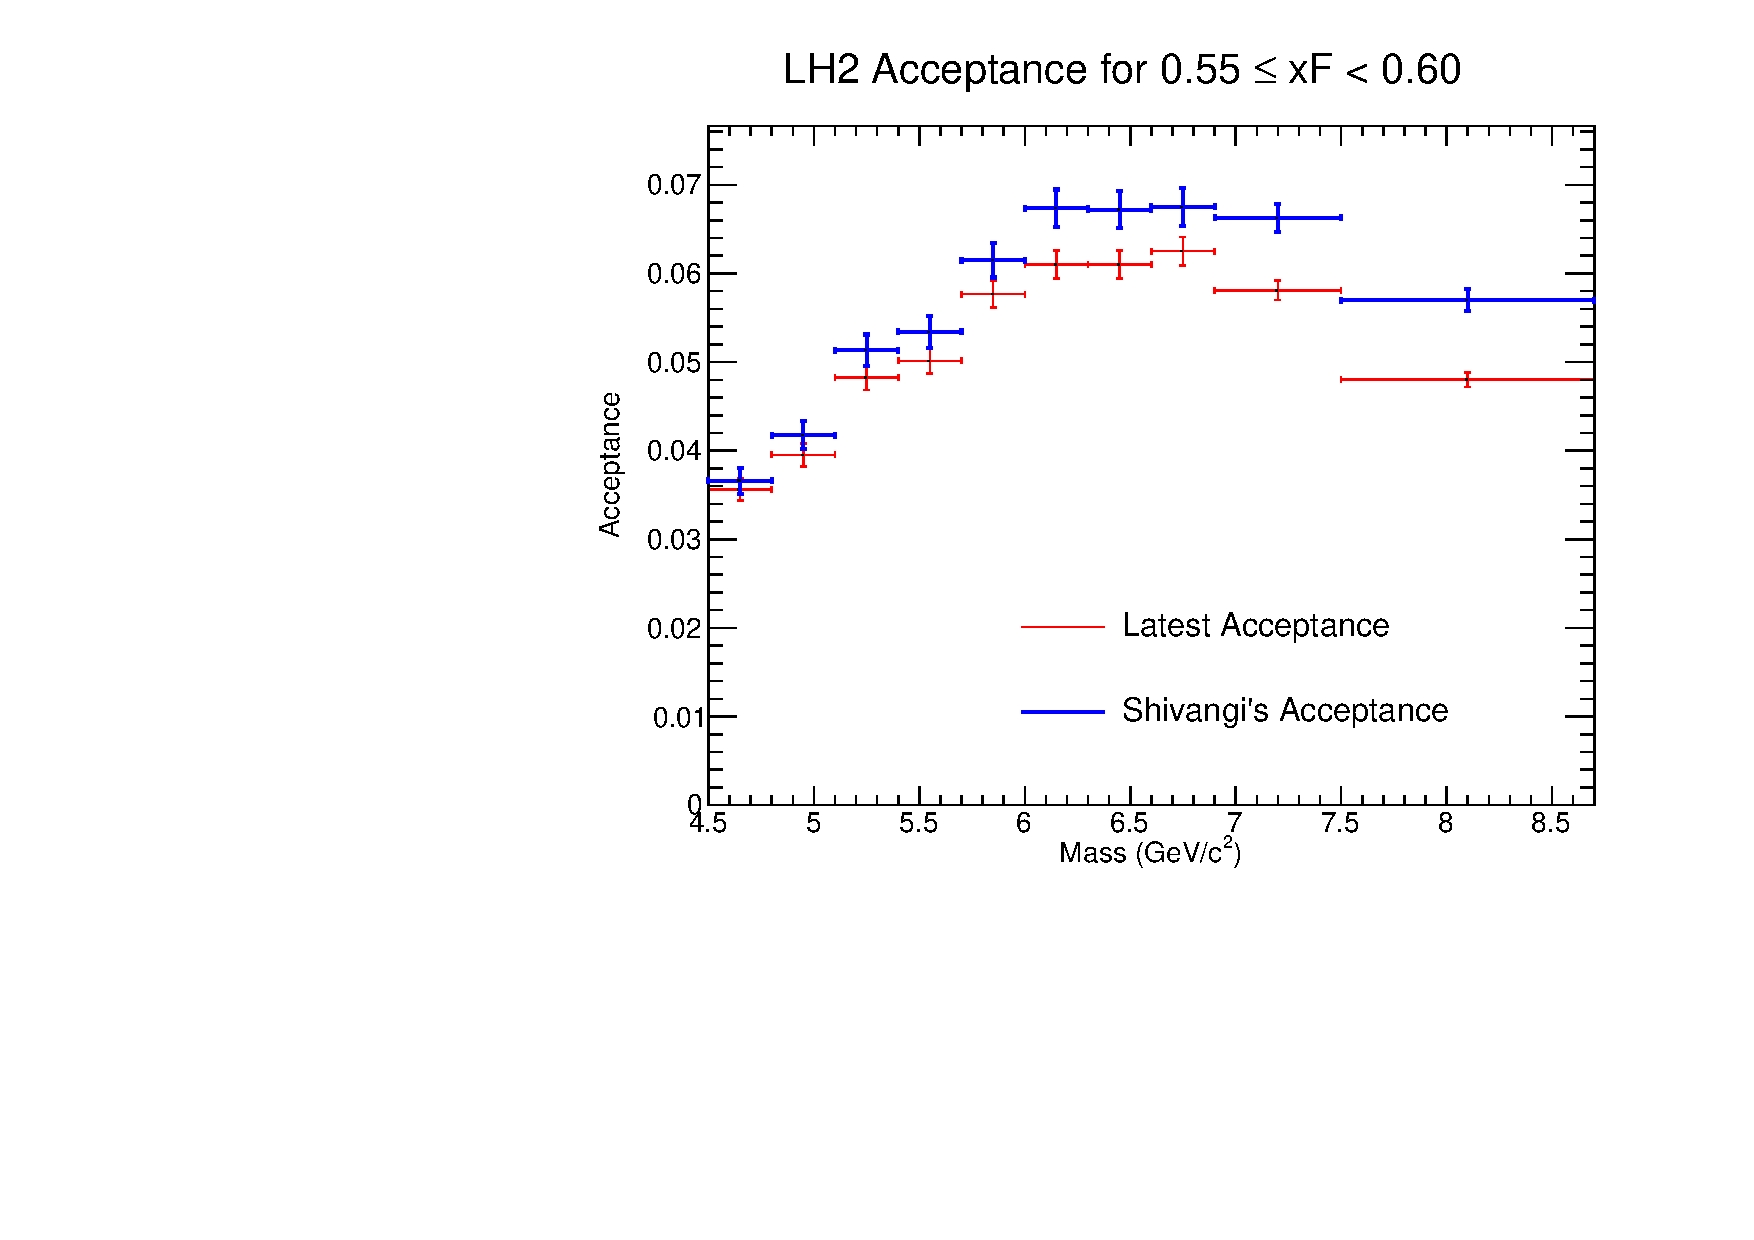
\includegraphics[width=\linewidth]{./acceptancePlots/LH2_acceptance_xF_bin_11.pdf}
       \caption{Acceptance for LH2}
    \end{subfigure}\hfill
    \begin{subfigure}[b]{0.48\textwidth}
       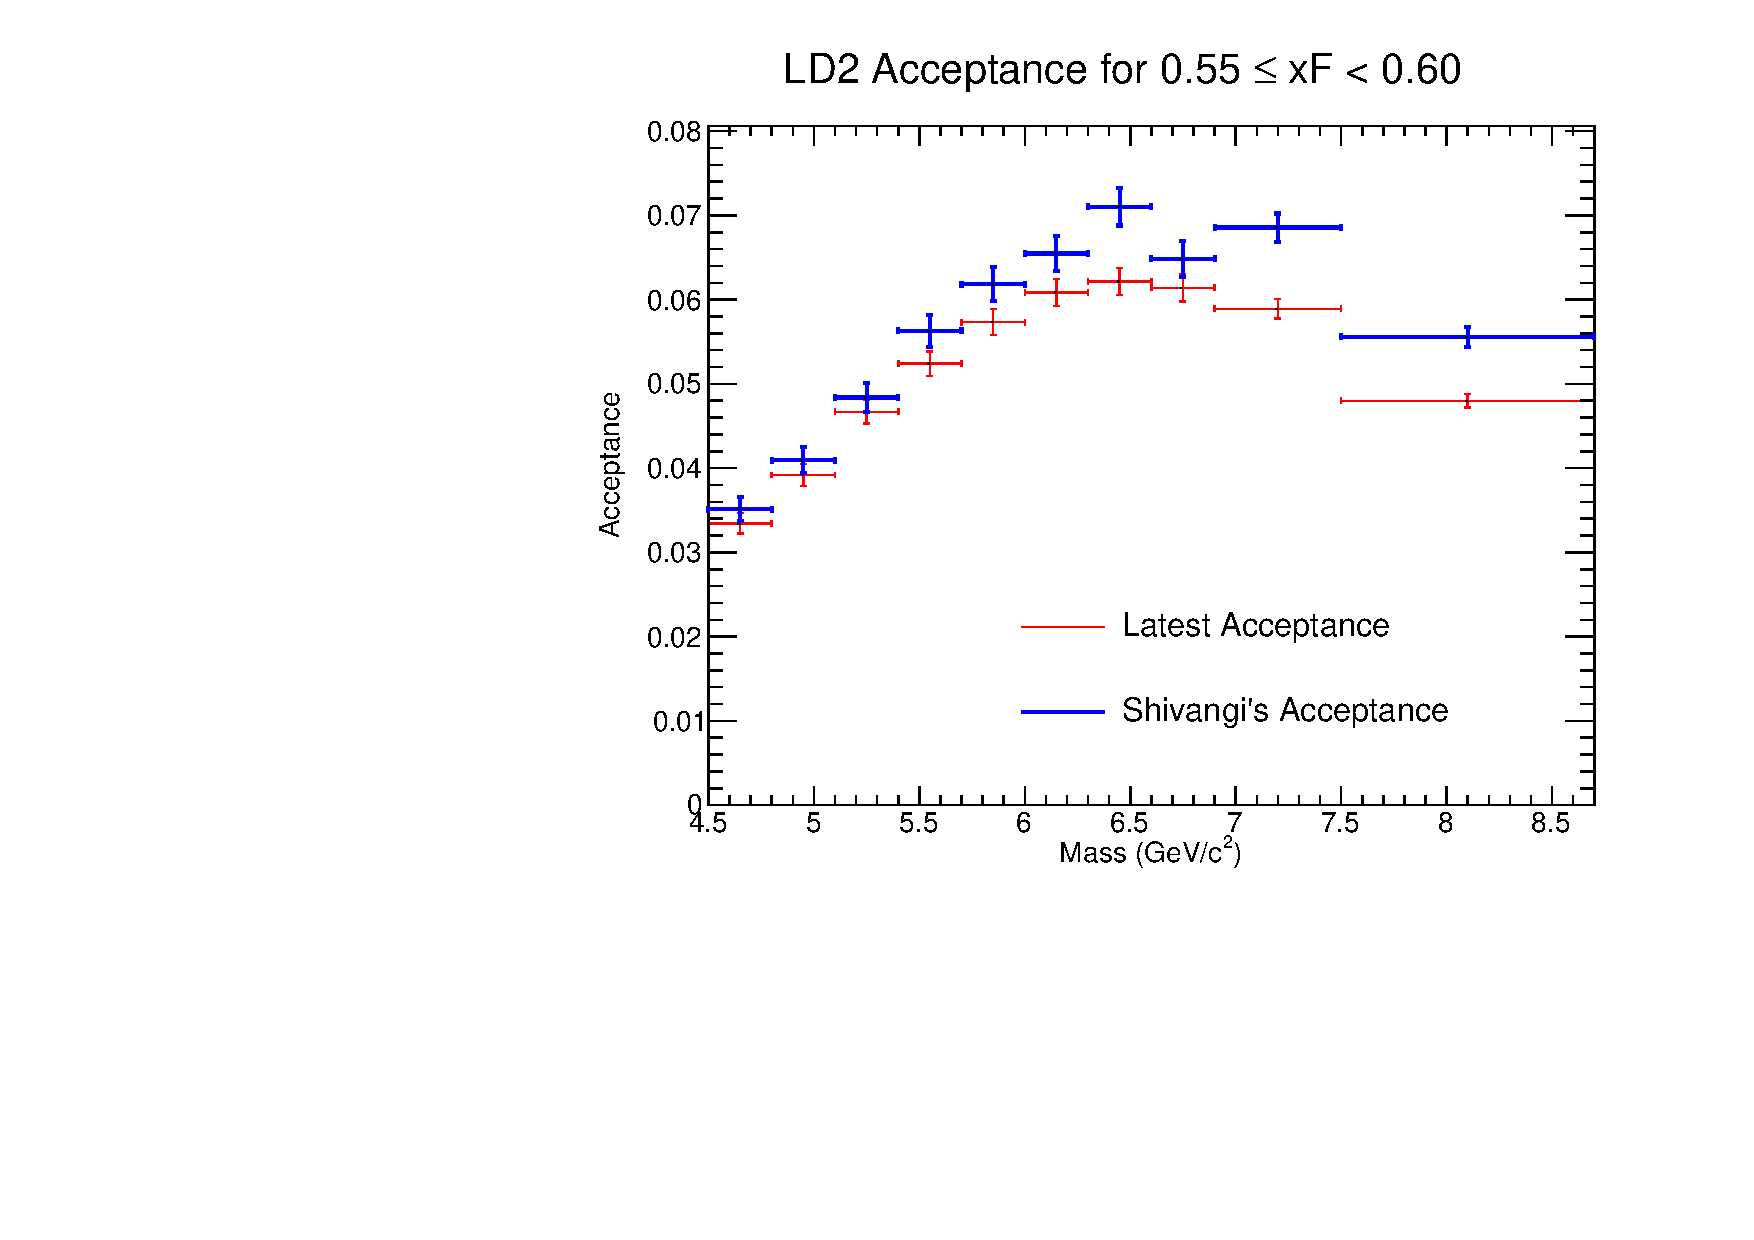
\includegraphics[width=\linewidth]{./acceptancePlots/LD2_acceptance_xF_bin_11.pdf}
       \caption{Acceptance for LD2}
    \end{subfigure}
    \begin{subfigure}[b]{0.48\textwidth}
       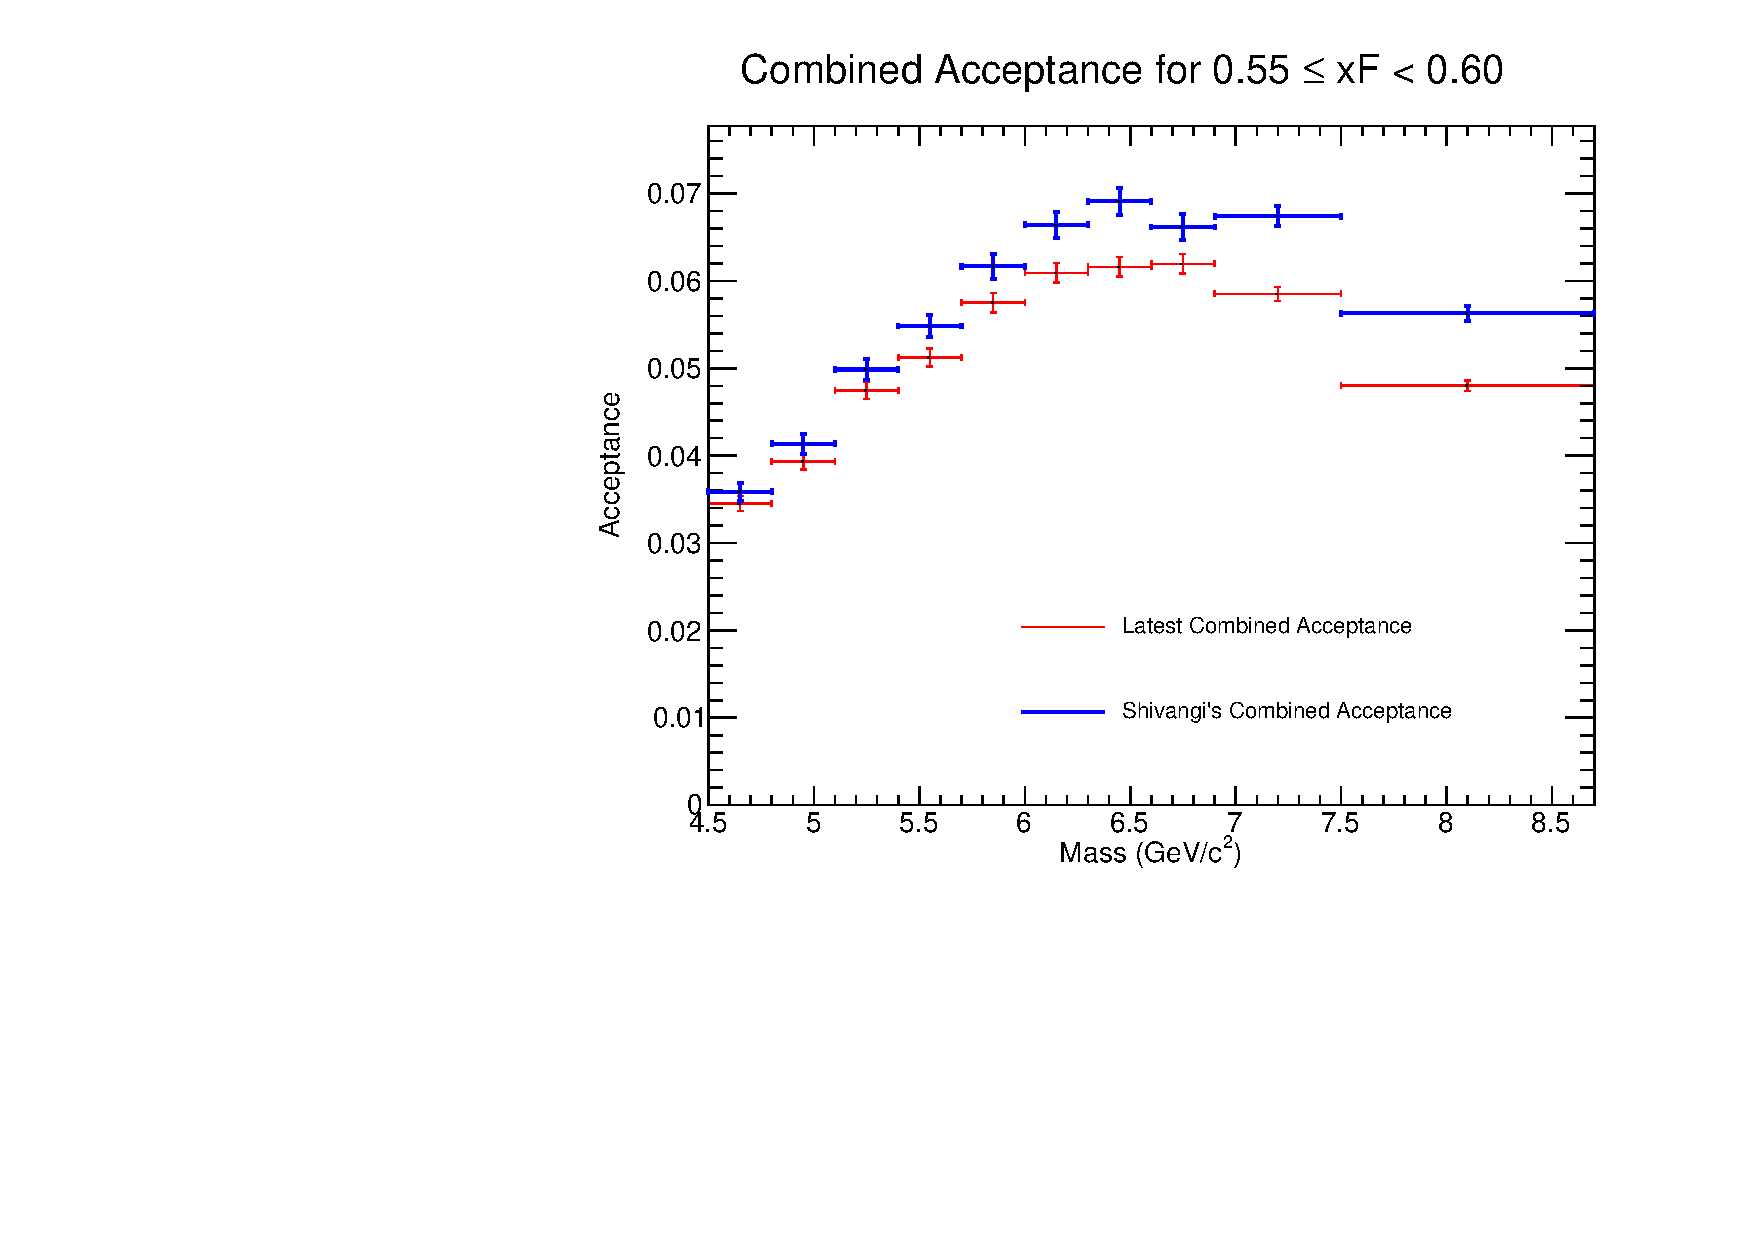
\includegraphics[width=\linewidth]{./acceptancePlots/Combined_acceptance_xF_bin_11.pdf}
       \caption{Combined Acceptance}
    \end{subfigure}\hfill
    \begin{subfigure}[b]{0.48\textwidth}
       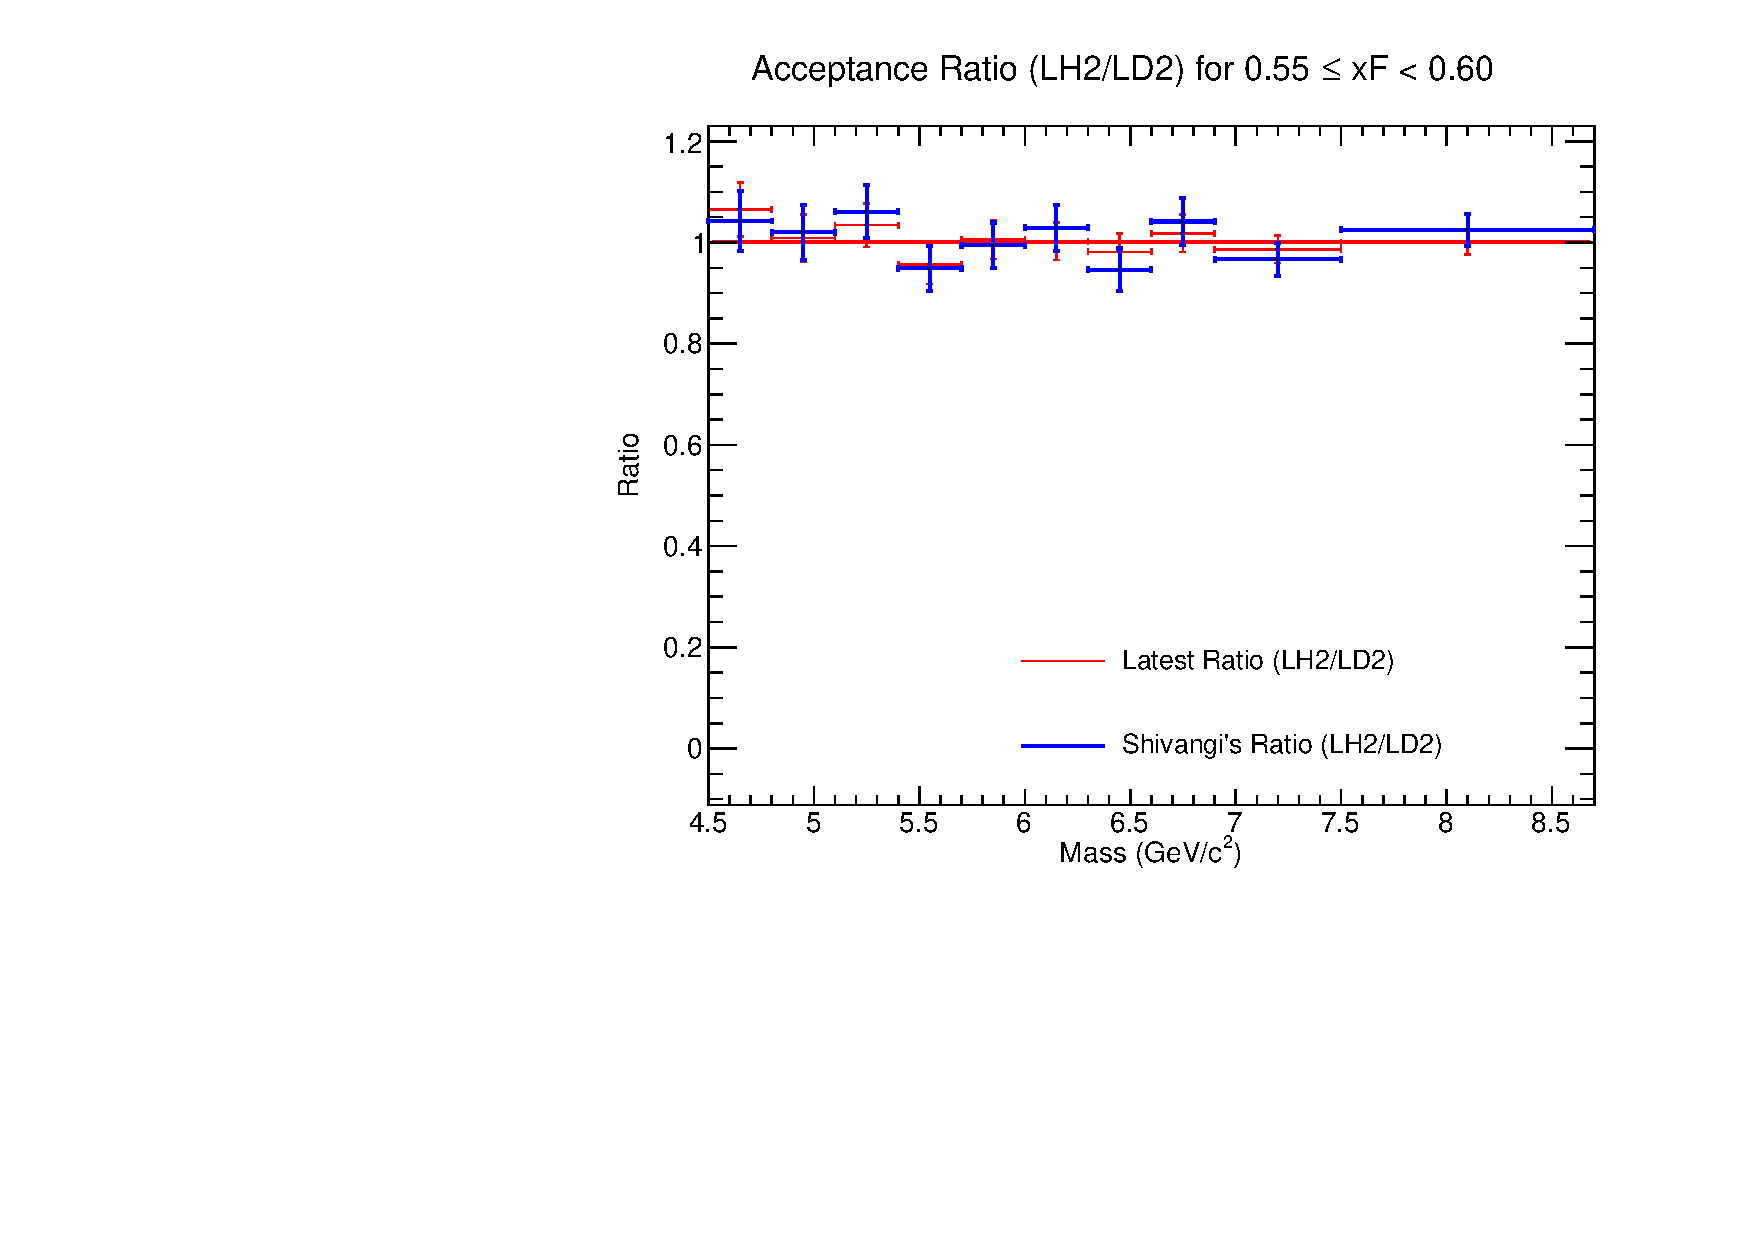
\includegraphics[width=\linewidth]{./acceptancePlots/Acceptance_ratio_xF_bin_11.pdf}
       \caption{Acceptance Ratio (LH2/LD2)}
    \end{subfigure}
    \caption{Acceptance plots for $0.55 \le x_F < 0.60$.}
\end{figure}

\begin{figure}[p]
    \centering
    \begin{subfigure}[b]{0.48\textwidth}
       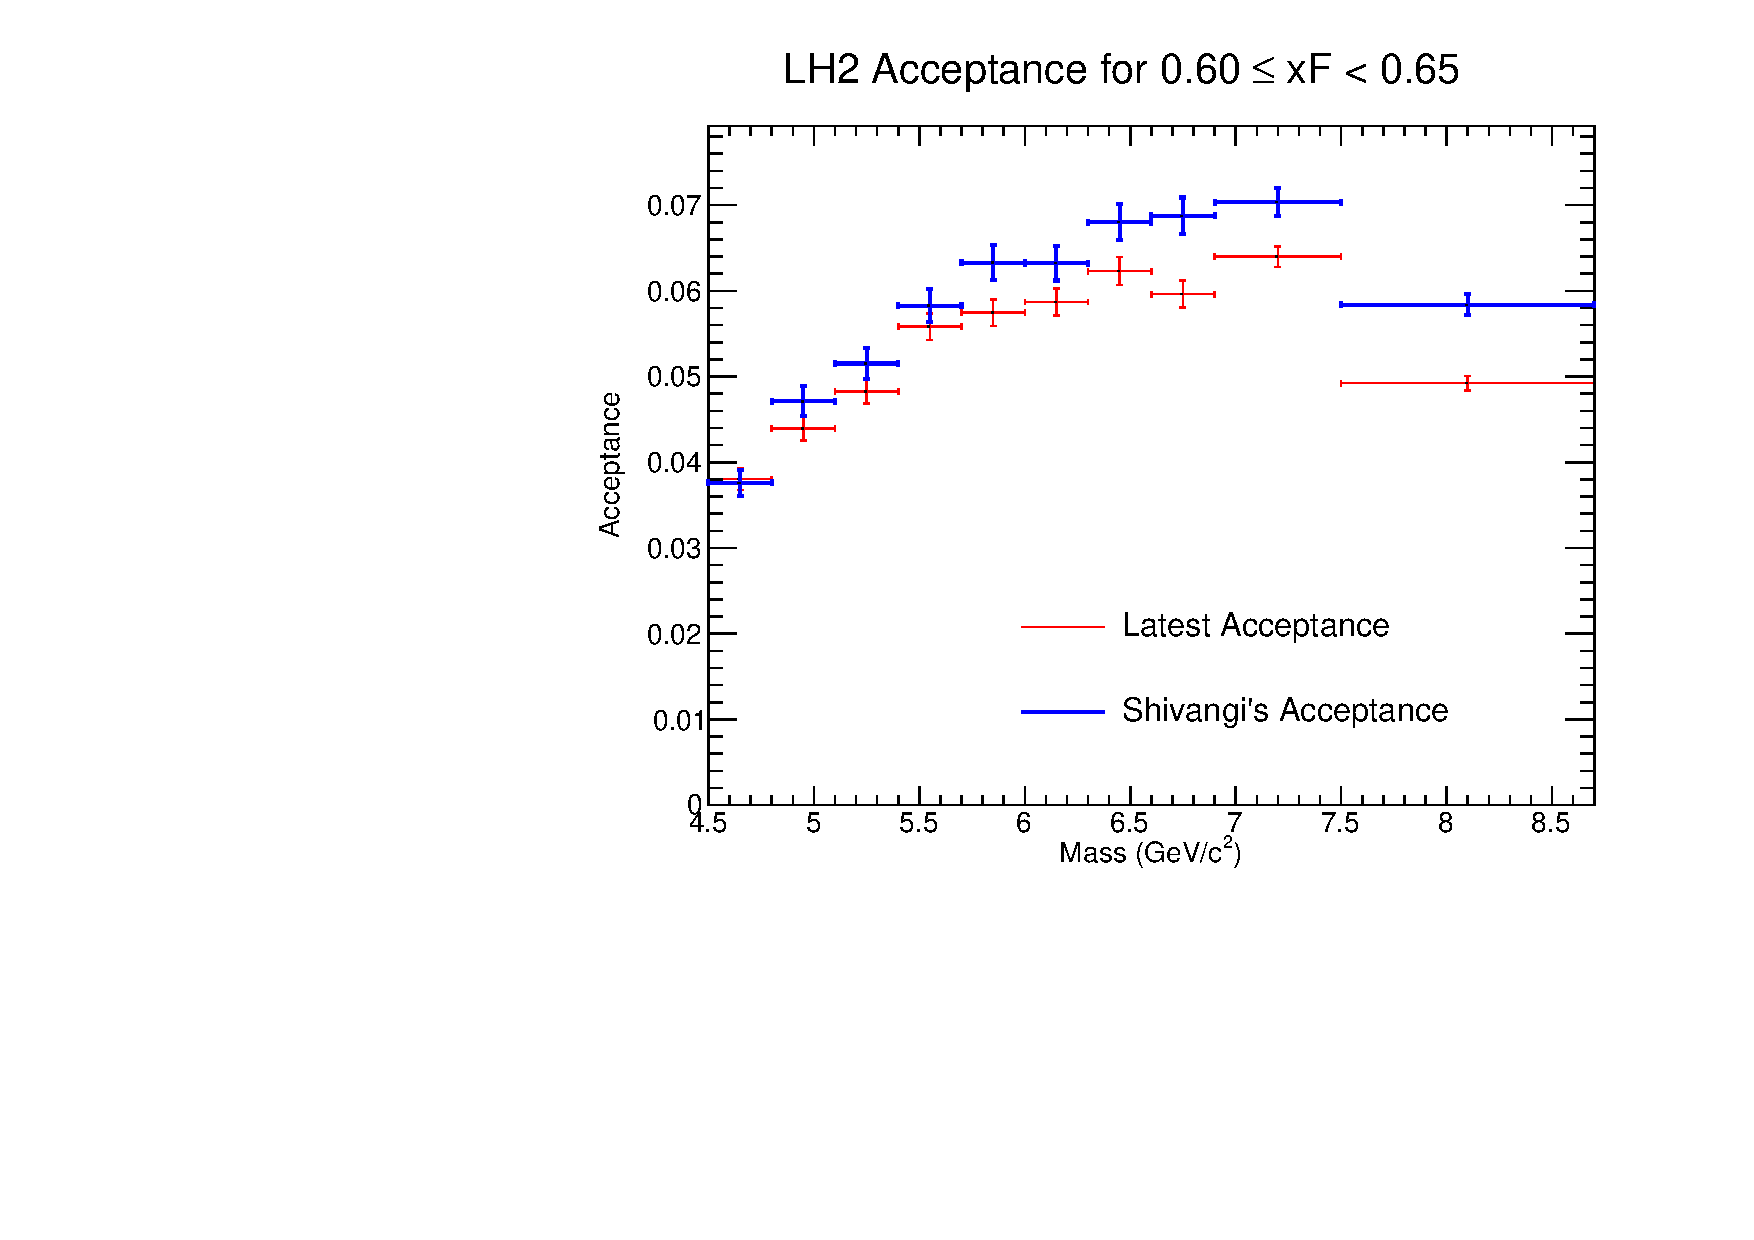
\includegraphics[width=\linewidth]{./acceptancePlots/LH2_acceptance_xF_bin_12.pdf}
       \caption{Acceptance for LH2}
    \end{subfigure}\hfill
    \begin{subfigure}[b]{0.48\textwidth}
       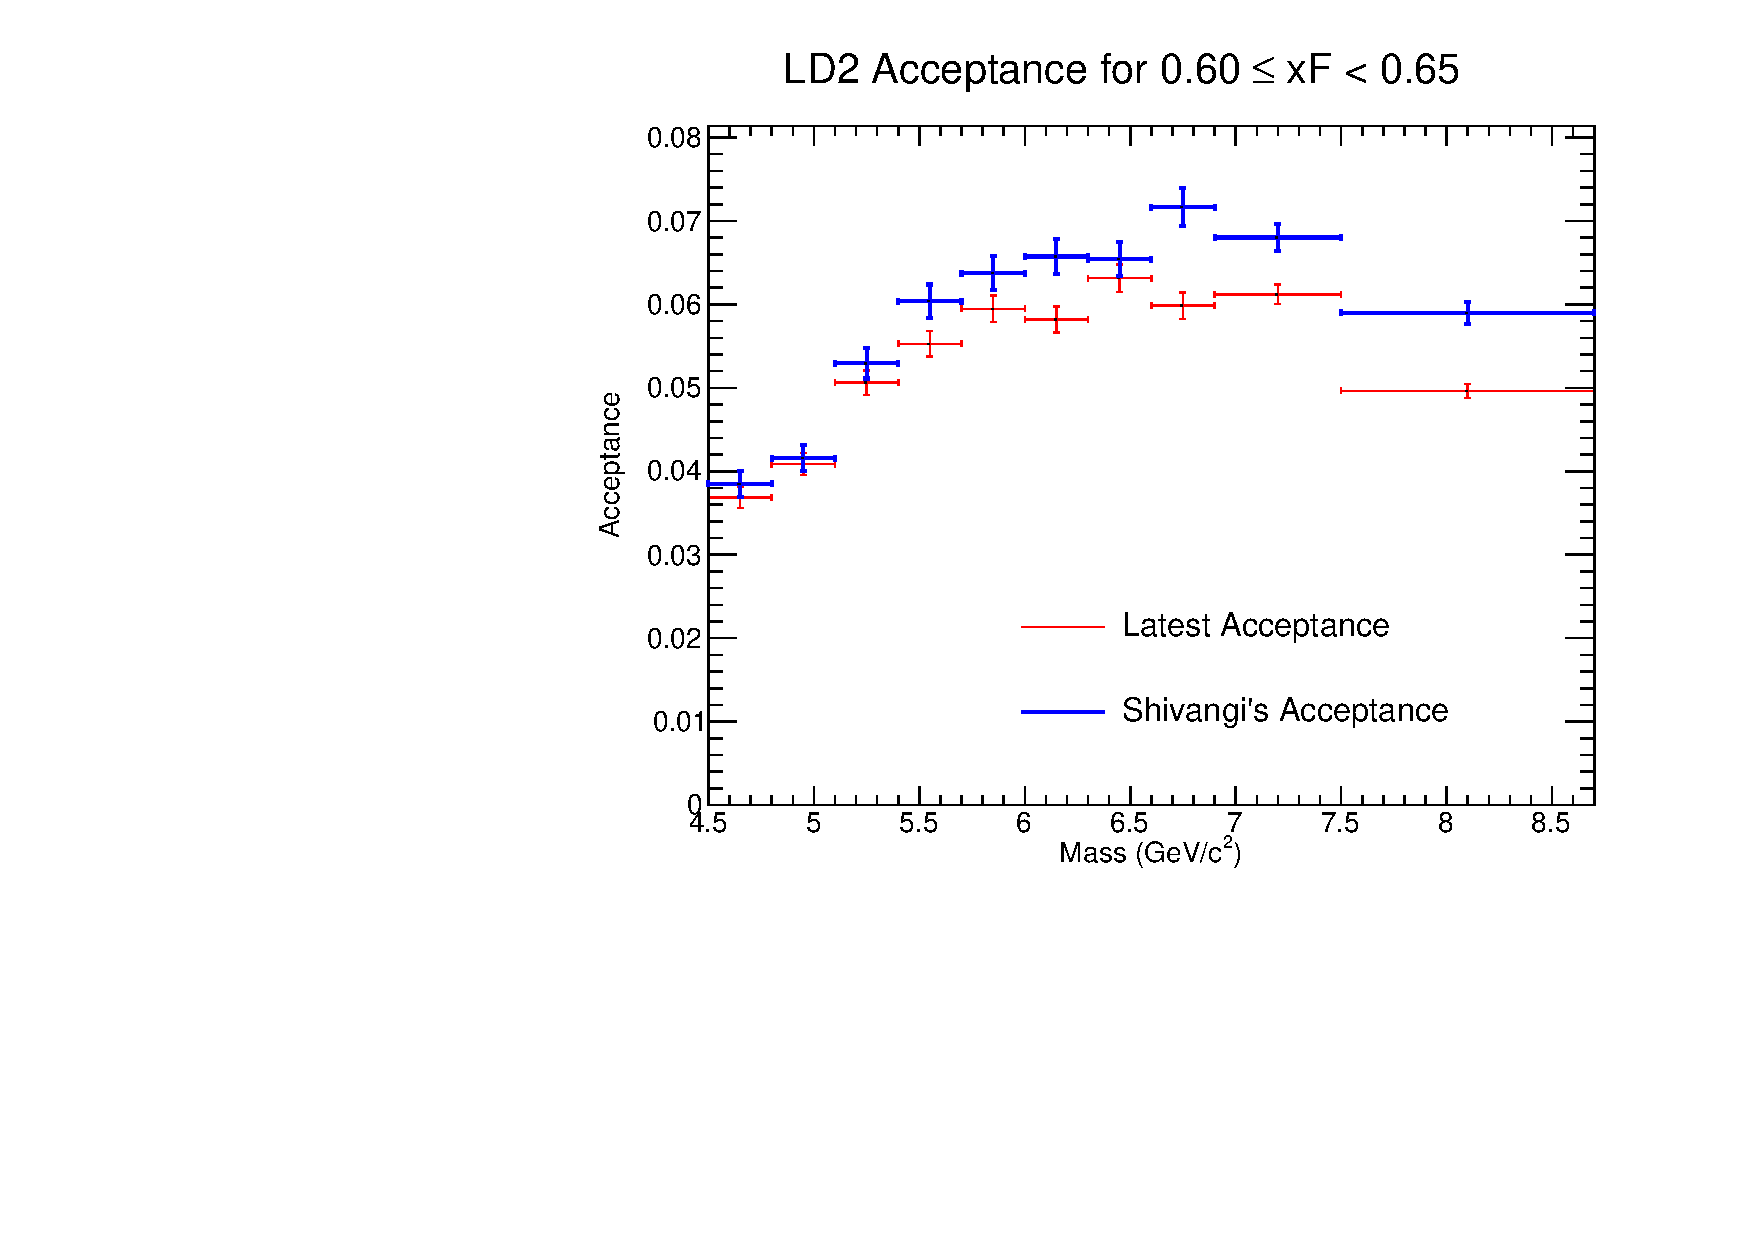
\includegraphics[width=\linewidth]{./acceptancePlots/LD2_acceptance_xF_bin_12.pdf}
       \caption{Acceptance for LD2}
    \end{subfigure}
    \begin{subfigure}[b]{0.48\textwidth}
       \includegraphics[width=\linewidth]{./acceptancePlots/Combined_acceptance_xF_bin_12.pdf}
       \caption{Combined Acceptance}
    \end{subfigure}\hfill
    \begin{subfigure}[b]{0.48\textwidth}
       \includegraphics[width=\linewidth]{./acceptancePlots/Acceptance_ratio_xF_bin_12.pdf}
       \caption{Acceptance Ratio (LH2/LD2)}
    \end{subfigure}
    \caption{Acceptance plots for $0.60 \le x_F < 0.65$.}
\end{figure}

\begin{figure}[p]
    \centering
    \begin{subfigure}[b]{0.48\textwidth}
       \includegraphics[width=\linewidth]{./acceptancePlots/LH2_acceptance_xF_bin_13.pdf}
       \caption{Acceptance for LH2}
    \end{subfigure}\hfill
    \begin{subfigure}[b]{0.48\textwidth}
       \includegraphics[width=\linewidth]{./acceptancePlots/LD2_acceptance_xF_bin_13.pdf}
       \caption{Acceptance for LD2}
    \end{subfigure}
    \begin{subfigure}[b]{0.48\textwidth}
       \includegraphics[width=\linewidth]{./acceptancePlots/Combined_acceptance_xF_bin_13.pdf}
       \caption{Combined Acceptance}
    \end{subfigure}\hfill
    \begin{subfigure}[b]{0.48\textwidth}
       \includegraphics[width=\linewidth]{./acceptancePlots/Acceptance_ratio_xF_bin_13.pdf}
       \caption{Acceptance Ratio (LH2/LD2)}
    \end{subfigure}
    \caption{Acceptance plots for $0.65 \le x_F < 0.70$.}
\end{figure}

\begin{figure}[p]
    \centering
    \begin{subfigure}[b]{0.48\textwidth}
       \includegraphics[width=\linewidth]{./acceptancePlots/LH2_acceptance_xF_bin_14.pdf}
       \caption{Acceptance for LH2}
    \end{subfigure}\hfill
    \begin{subfigure}[b]{0.48\textwidth}
       \includegraphics[width=\linewidth]{./acceptancePlots/LD2_acceptance_xF_bin_14.pdf}
       \caption{Acceptance for LD2}
    \end{subfigure}
    \begin{subfigure}[b]{0.48\textwidth}
       \includegraphics[width=\linewidth]{./acceptancePlots/Combined_acceptance_xF_bin_14.pdf}
       \caption{Combined Acceptance}
    \end{subfigure}\hfill
    \begin{subfigure}[b]{0.48\textwidth}
       \includegraphics[width=\linewidth]{./acceptancePlots/Acceptance_ratio_xF_bin_14.pdf}
       \caption{Acceptance Ratio (LH2/LD2)}
    \end{subfigure}
    \caption{Acceptance plots for $0.70 \le x_F < 0.75$.}
\end{figure}

\begin{figure}[p]
    \centering
    \begin{subfigure}[b]{0.48\textwidth}
       \includegraphics[width=\linewidth]{./acceptancePlots/LH2_acceptance_xF_bin_15.pdf}
       \caption{Acceptance for LH2}
    \end{subfigure}\hfill
    \begin{subfigure}[b]{0.48\textwidth}
       \includegraphics[width=\linewidth]{./acceptancePlots/LD2_acceptance_xF_bin_15.pdf}
       \caption{Acceptance for LD2}
    \end{subfigure}
    \begin{subfigure}[b]{0.48\textwidth}
       \includegraphics[width=\linewidth]{./acceptancePlots/Combined_acceptance_xF_bin_15.pdf}
       \caption{Combined Acceptance}
    \end{subfigure}\hfill
    \begin{subfigure}[b]{0.48\textwidth}
       \includegraphics[width=\linewidth]{./acceptancePlots/Acceptance_ratio_xF_bin_15.pdf}
       \caption{Acceptance Ratio (LH2/LD2)}
    \end{subfigure}
    \caption{Acceptance plots for $0.75 \le x_F < 0.80$.}
\end{figure}

\FloatBarrier

\subsection{Reconstruction Efficiency Correction}
\label{sec:ktracker_eff}
The track-finding algorithm ("kTracker") has an efficiency that depends on the detector occupancy; the number of hits from unrelated particles in the detector during an event. This efficiency is studied using "clean" MC simulations (signal only) and "messy" MC simulations (signal with background hits overlaid). The reconstruction efficiency, $\epsilon_{\text{recon}}$, is defined as the ratio of events found in the messy sample to those in the clean sample, as a function of an occupancy-related variable (e.g., D2, the number of hits in Drift Chamber Station 2).

\begin{equation}
    \epsilon_{\text{recon}}(\text{D2}, M, x_F) = \frac{N_{\text{reco}}^{\text{messy}}(\text{D2}, M, x_F)}{N_{\text{reco}}^{\text{clean}}(M, x_F)}
\end{equation}

For each kinematic bin of ($M, x_F$), an efficiency curve as a function of D2 is generated from the MC. To obtain a single correction factor for each bin, an average efficiency, $\langle \epsilon \rangle$, is calculated by weighting this efficiency curve by the D2 distribution of the experimental data in that same bin.

\subsubsection{Uncertainty Propagation}
An important aspect of this procedure is the correct propagation of uncertainties. For each event in the data with a measured D2 value, an efficiency $\epsilon_{i}$ and its uncertainty $\delta\epsilon_{i}$ are determined by linear interpolation between points on the MC-derived efficiency curve.  For a given event $i$ the efficiency will be interpolated:
$$\epsilon_i = \epsilon(D2^-)+\left(\frac{\epsilon(D2^+)-\epsilon(D2^-)}{D2^+-D2^-} \right)\left(D2^+-D2_i\right) $$
$$\delta\epsilon_i = \frac{1}{D2^+-D2^-}\sqrt{\left(D2^+-D2_i\right)^2\delta\epsilon(D2^+)^2+\left(D2^--D2_i\right)^2\delta\epsilon(D2^-)^2}$$
where $D2_i$ is the value of D2 for the event $i$, $D2^+$ is the nearest D2 value greater than $D2_i$, $D2^-$ is the nearest D2 value less than $D2_i$, $\epsilon(D2^\pm)$ is the value of the efficiency at $D2^\pm$, and $\delta\epsilon(D2^\pm)$ is the uncertainty in $\epsilon(D2^\pm)$

The average efficiency $\langle\epsilon\rangle$ for a bin containing $N$ data events is the mean of the individual efficiencies:
\begin{equation} \label{eq:avg_eff_2}
    \langle\epsilon\rangle = \frac{1}{N} \sum_{i=1}^{N} \epsilon_i
\end{equation}

The uncertainty on this average, $\delta\langle\epsilon\rangle$, is based on the propagated error from the uncertainty on the MC-derived efficiency curve itself. 
\begin{equation} \label{eq:prop_err_2}
    \delta_{\text{prop}} \langle\epsilon\rangle = \frac{1}{N} \sqrt{\sum_{i=1}^{N} (\delta\epsilon_i)^2}
\end{equation}
The final correction applied to the data is $1/\langle\epsilon\rangle$, and its propagated error is given by:
\begin{equation} \label{eq:inv_err_2}
    \delta(1/\langle\epsilon\rangle) = \frac{\delta_{\text{prop}}\langle\epsilon\rangle}{\langle\epsilon\rangle^2}
\end{equation}

\subsubsection{Efficiency Results}
The efficiency curves as a function of D2 were generated for all kinematic bins. The following pages display these curves, with each page corresponding to a single bin in $x_F$, showing the results for all 11 mass bins.  {\bf It is clear that some bins have insufficient statistics, and we should perform additional MC simulation in the near future to remedy this.} The efficiency sometimes exceeds 1.0 due to mistakenly reconstructing dimuon events due to ``messy pick-up events'' for some D2 bins.

%--- All Efficiency plots ---
\begin{figure}[p]
    \centering
    \begin{subfigure}[b]{0.32\textwidth}
        \centering
        \includegraphics[width=\textwidth]{./kTrackerEfficiencyPlots/D2_Efficiency_xF0_mass0.pdf}
        \caption{$4.2 \leq m < 4.5$ GeV/$c^2$}
    \end{subfigure}\hfill
    \begin{subfigure}[b]{0.32\textwidth}
        \centering
        \includegraphics[width=\textwidth]{./kTrackerEfficiencyPlots/D2_Efficiency_xF0_mass1.pdf}
        \caption{$4.5 \leq m < 4.8$ GeV/$c^2$}
    \end{subfigure}\hfill
    \begin{subfigure}[b]{0.32\textwidth}
        \centering
        \includegraphics[width=\textwidth]{./kTrackerEfficiencyPlots/D2_Efficiency_xF0_mass2.png}
        \caption{$4.8 \leq m < 5.1$ GeV/$c^2$}
    \end{subfigure}\vspace{0.5cm}
    \begin{subfigure}[b]{0.32\textwidth}
        \centering
        \includegraphics[width=\textwidth]{./kTrackerEfficiencyPlots/D2_Efficiency_xF0_mass3.pdf}
        \caption{$5.1 \leq m < 5.4$ GeV/$c^2$}
    \end{subfigure}\hfill
    \begin{subfigure}[b]{0.32\textwidth}
        \centering
        \includegraphics[width=\textwidth]{./kTrackerEfficiencyPlots/D2_Efficiency_xF0_mass4.png}
        \caption{$5.4 \leq m < 5.7$ GeV/$c^2$}
    \end{subfigure}\hfill
    \begin{subfigure}[b]{0.32\textwidth}
        \centering
        \includegraphics[width=\textwidth]{./kTrackerEfficiencyPlots/D2_Efficiency_xF0_mass5.pdf}
        \caption{$5.7 \leq m < 6.0$ GeV/$c^2$}
    \end{subfigure}\vspace{0.5cm}
    \begin{subfigure}[b]{0.32\textwidth}
        \centering
        \includegraphics[width=\textwidth]{./kTrackerEfficiencyPlots/D2_Efficiency_xF0_mass6.pdf}
        \caption{$6.0 \leq m < 6.3$ GeV/$c^2$}
    \end{subfigure}\hfill
    \begin{subfigure}[b]{0.32\textwidth}
        \centering
        \includegraphics[width=\textwidth]{./kTrackerEfficiencyPlots/D2_Efficiency_xF0_mass7.png}
        \caption{$6.3 \leq m < 6.6$ GeV/$c^2$}
    \end{subfigure}\hfill
    \begin{subfigure}[b]{0.32\textwidth}
        \centering
        \includegraphics[width=\textwidth]{./kTrackerEfficiencyPlots/D2_Efficiency_xF0_mass8.pdf}
        \caption{$6.6 \leq m < 6.9$ GeV/$c^2$}
    \end{subfigure}\vspace{0.5cm}
    \begin{subfigure}[b]{0.32\textwidth}
        \centering
        \includegraphics[width=\textwidth]{./kTrackerEfficiencyPlots/D2_Efficiency_xF0_mass9.pdf}
        \caption{$6.9 \leq m < 7.5$ GeV/$c^2$}
    \end{subfigure}\hfill
    \begin{subfigure}[b]{0.32\textwidth}
        \centering
        \includegraphics[width=\textwidth]{./kTrackerEfficiencyPlots/D2_Efficiency_xF0_mass10.pdf}
        \caption{$7.5 \leq m < 8.7$ GeV/$c^2$}
    \end{subfigure}
    \caption{Efficiency plots for the $x_F$ bin $0.00 \leq x_F < 0.05$.}
\end{figure}

\begin{figure}[p]
    \centering
    \begin{subfigure}[b]{0.32\textwidth}
        \centering
        \includegraphics[width=\textwidth]{./kTrackerEfficiencyPlots/D2_Efficiency_xF1_mass0.pdf}
        \caption{$4.2 \leq m < 4.5$ GeV/$c^2$}
    \end{subfigure}\hfill
    \begin{subfigure}[b]{0.32\textwidth}
        \centering
        \includegraphics[width=\textwidth]{./kTrackerEfficiencyPlots/D2_Efficiency_xF1_mass1.png}
        \caption{$4.5 \leq m < 4.8$ GeV/$c^2$}
    \end{subfigure}\hfill
    \begin{subfigure}[b]{0.32\textwidth}
        \centering
        \includegraphics[width=\textwidth]{./kTrackerEfficiencyPlots/D2_Efficiency_xF1_mass2.pdf}
        \caption{$4.8 \leq m < 5.1$ GeV/$c^2$}
    \end{subfigure}\vspace{0.5cm}
    \begin{subfigure}[b]{0.32\textwidth}
        \centering
        \includegraphics[width=\textwidth]{./kTrackerEfficiencyPlots/D2_Efficiency_xF1_mass3.pdf}
        \caption{$5.1 \leq m < 5.4$ GeV/$c^2$}
    \end{subfigure}\hfill
    \begin{subfigure}[b]{0.32\textwidth}
        \centering
        \includegraphics[width=\textwidth]{./kTrackerEfficiencyPlots/D2_Efficiency_xF1_mass4.png}
        \caption{$5.4 \leq m < 5.7$ GeV/$c^2$}
    \end{subfigure}\hfill
    \begin{subfigure}[b]{0.32\textwidth}
        \centering
        \includegraphics[width=\textwidth]{./kTrackerEfficiencyPlots/D2_Efficiency_xF1_mass5.pdf}
        \caption{$5.7 \leq m < 6.0$ GeV/$c^2$}
    \end{subfigure}\vspace{0.5cm}
    \begin{subfigure}[b]{0.32\textwidth}
        \centering
        \includegraphics[width=\textwidth]{./kTrackerEfficiencyPlots/D2_Efficiency_xF1_mass6.pdf}
        \caption{$6.0 \leq m < 6.3$ GeV/$c^2$}
    \end{subfigure}\hfill
    \begin{subfigure}[b]{0.32\textwidth}
        \centering
        \includegraphics[width=\textwidth]{./kTrackerEfficiencyPlots/D2_Efficiency_xF1_mass7.pdf}
        \caption{$6.3 \leq m < 6.6$ GeV/$c^2$}
    \end{subfigure}\hfill
    \begin{subfigure}[b]{0.32\textwidth}
        \centering
        \includegraphics[width=\textwidth]{./kTrackerEfficiencyPlots/D2_Efficiency_xF1_mass8.pdf}
        \caption{$6.6 \leq m < 6.9$ GeV/$c^2$}
    \end{subfigure}\vspace{0.5cm}
    \begin{subfigure}[b]{0.32\textwidth}
        \centering
        \includegraphics[width=\textwidth]{./kTrackerEfficiencyPlots/D2_Efficiency_xF1_mass9.pdf}
        \caption{$6.9 \leq m < 7.5$ GeV/$c^2$}
    \end{subfigure}\hfill
    \begin{subfigure}[b]{0.32\textwidth}
        \centering
        \includegraphics[width=\textwidth]{./kTrackerEfficiencyPlots/D2_Efficiency_xF1_mass10.pdf}
        \caption{$7.5 \leq m < 8.7$ GeV/$c^2$}
    \end{subfigure}
    \caption{Efficiency plots for the $x_F$ bin $0.05 \leq x_F < 0.10$.}
\end{figure}

\begin{figure}[p]
    \centering
    \begin{subfigure}[b]{0.32\textwidth}
        \centering
        \includegraphics[width=\textwidth]{./kTrackerEfficiencyPlots/D2_Efficiency_xF2_mass0.pdf}
        \caption{$4.2 \leq m < 4.5$ GeV/$c^2$}
    \end{subfigure}\hfill
    \begin{subfigure}[b]{0.32\textwidth}
        \centering
        \includegraphics[width=\textwidth]{./kTrackerEfficiencyPlots/D2_Efficiency_xF2_mass1.pdf}
        \caption{$4.5 \leq m < 4.8$ GeV/$c^2$}
    \end{subfigure}\hfill
    \begin{subfigure}[b]{0.32\textwidth}
        \centering
        \includegraphics[width=\textwidth]{./kTrackerEfficiencyPlots/D2_Efficiency_xF2_mass2.png}
        \caption{$4.8 \leq m < 5.1$ GeV/$c^2$}
    \end{subfigure}\vspace{0.5cm}
    \begin{subfigure}[b]{0.32\textwidth}
        \centering
        \includegraphics[width=\textwidth]{./kTrackerEfficiencyPlots/D2_Efficiency_xF2_mass3.pdf}
        \caption{$5.1 \leq m < 5.4$ GeV/$c^2$}
    \end{subfigure}\hfill
    \begin{subfigure}[b]{0.32\textwidth}
        \centering
        \includegraphics[width=\textwidth]{./kTrackerEfficiencyPlots/D2_Efficiency_xF2_mass4.pdf}
        \caption{$5.4 \leq m < 5.7$ GeV/$c^2$}
    \end{subfigure}\hfill
    \begin{subfigure}[b]{0.32\textwidth}
        \centering
        \includegraphics[width=\textwidth]{./kTrackerEfficiencyPlots/D2_Efficiency_xF2_mass5.pdf}
        \caption{$5.7 \leq m < 6.0$ GeV/$c^2$}
    \end{subfigure}\vspace{0.5cm}
    \begin{subfigure}[b]{0.32\textwidth}
        \centering
        \includegraphics[width=\textwidth]{./kTrackerEfficiencyPlots/D2_Efficiency_xF2_mass6.png}
        \caption{$6.0 \leq m < 6.3$ GeV/$c^2$}
    \end{subfigure}\hfill
    \begin{subfigure}[b]{0.32\textwidth}
        \centering
        \includegraphics[width=\textwidth]{./kTrackerEfficiencyPlots/D2_Efficiency_xF2_mass7.pdf}
        \caption{$6.3 \leq m < 6.6$ GeV/$c^2$}
    \end{subfigure}\hfill
    \begin{subfigure}[b]{0.32\textwidth}
        \centering
        \includegraphics[width=\textwidth]{./kTrackerEfficiencyPlots/D2_Efficiency_xF2_mass8.pdf}
        \caption{$6.6 \leq m < 6.9$ GeV/$c^2$}
    \end{subfigure}\vspace{0.5cm}
    \begin{subfigure}[b]{0.32\textwidth}
        \centering
        \includegraphics[width=\textwidth]{./kTrackerEfficiencyPlots/D2_Efficiency_xF2_mass9.pdf}
        \caption{$6.9 \leq m < 7.5$ GeV/$c^2$}
    \end{subfigure}\hfill
    \begin{subfigure}[b]{0.32\textwidth}
        \centering
        \includegraphics[width=\textwidth]{./kTrackerEfficiencyPlots/D2_Efficiency_xF2_mass10.pdf}
        \caption{$7.5 \leq m < 8.7$ GeV/$c^2$}
    \end{subfigure}
    \caption{Efficiency plots for the $x_F$ bin $0.10 \leq x_F < 0.15$.}
\end{figure}

\begin{figure}[p]
    \centering
    \begin{subfigure}[b]{0.32\textwidth}
        \centering
        \includegraphics[width=\textwidth]{./kTrackerEfficiencyPlots/D2_Efficiency_xF3_mass0.pdf}
        \caption{$4.2 \leq m < 4.5$ GeV/$c^2$}
    \end{subfigure}\hfill
    \begin{subfigure}[b]{0.32\textwidth}
        \centering
        \includegraphics[width=\textwidth]{./kTrackerEfficiencyPlots/D2_Efficiency_xF3_mass1.pdf}
        \caption{$4.5 \leq m < 4.8$ GeV/$c^2$}
    \end{subfigure}\hfill
    \begin{subfigure}[b]{0.32\textwidth}
        \centering
        \includegraphics[width=\textwidth]{./kTrackerEfficiencyPlots/D2_Efficiency_xF3_mass2.pdf}
        \caption{$4.8 \leq m < 5.1$ GeV/$c^2$}
    \end{subfigure}\vspace{0.5cm}
    \begin{subfigure}[b]{0.32\textwidth}
        \centering
        \includegraphics[width=\textwidth]{./kTrackerEfficiencyPlots/D2_Efficiency_xF3_mass3.png}
        \caption{$5.1 \leq m < 5.4$ GeV/$c^2$}
    \end{subfigure}\hfill
    \begin{subfigure}[b]{0.32\textwidth}
        \centering
        \includegraphics[width=\textwidth]{./kTrackerEfficiencyPlots/D2_Efficiency_xF3_mass4.png}
        \caption{$5.4 \leq m < 5.7$ GeV/$c^2$}
    \end{subfigure}\hfill
    \begin{subfigure}[b]{0.32\textwidth}
        \centering
        \includegraphics[width=\textwidth]{./kTrackerEfficiencyPlots/D2_Efficiency_xF3_mass5.pdf}
        \caption{$5.7 \leq m < 6.0$ GeV/$c^2$}
    \end{subfigure}\vspace{0.5cm}
    \begin{subfigure}[b]{0.32\textwidth}
        \centering
        \includegraphics[width=\textwidth]{./kTrackerEfficiencyPlots/D2_Efficiency_xF3_mass6.pdf}
        \caption{$6.0 \leq m < 6.3$ GeV/$c^2$}
    \end{subfigure}\hfill
    \begin{subfigure}[b]{0.32\textwidth}
        \centering
        \includegraphics[width=\textwidth]{./kTrackerEfficiencyPlots/D2_Efficiency_xF3_mass7.png}
        \caption{$6.3 \leq m < 6.6$ GeV/$c^2$}
    \end{subfigure}\hfill
    \begin{subfigure}[b]{0.32\textwidth}
        \centering
        \includegraphics[width=\textwidth]{./kTrackerEfficiencyPlots/D2_Efficiency_xF3_mass8.png}
        \caption{$6.6 \leq m < 6.9$ GeV/$c^2$}
    \end{subfigure}\vspace{0.5cm}
    \begin{subfigure}[b]{0.32\textwidth}
        \centering
        \includegraphics[width=\textwidth]{./kTrackerEfficiencyPlots/D2_Efficiency_xF3_mass9.pdf}
        \caption{$6.9 \leq m < 7.5$ GeV/$c^2$}
    \end{subfigure}\hfill
    \begin{subfigure}[b]{0.32\textwidth}
        \centering
        \includegraphics[width=\textwidth]{./kTrackerEfficiencyPlots/D2_Efficiency_xF3_mass10.pdf}
        \caption{$7.5 \leq m < 8.7$ GeV/$c^2$}
    \end{subfigure}
    \caption{Efficiency plots for the $x_F$ bin $0.15 \leq x_F < 0.20$.}
\end{figure}

\begin{figure}[p]
    \centering
    \begin{subfigure}[b]{0.32\textwidth}
        \centering
        \includegraphics[width=\textwidth]{./kTrackerEfficiencyPlots/D2_Efficiency_xF4_mass0.pdf}
        \caption{$4.2 \leq m < 4.5$ GeV/$c^2$}
    \end{subfigure}\hfill
    \begin{subfigure}[b]{0.32\textwidth}
        \centering
        \includegraphics[width=\textwidth]{./kTrackerEfficiencyPlots/D2_Efficiency_xF4_mass1.pdf}
        \caption{$4.5 \leq m < 4.8$ GeV/$c^2$}
    \end{subfigure}\hfill
    \begin{subfigure}[b]{0.32\textwidth}
        \centering
        \includegraphics[width=\textwidth]{./kTrackerEfficiencyPlots/D2_Efficiency_xF4_mass2.pdf}
        \caption{$4.8 \leq m < 5.1$ GeV/$c^2$}
    \end{subfigure}\vspace{0.5cm}
    \begin{subfigure}[b]{0.32\textwidth}
        \centering
        \includegraphics[width=\textwidth]{./kTrackerEfficiencyPlots/D2_Efficiency_xF4_mass3.pdf}
        \caption{$5.1 \leq m < 5.4$ GeV/$c^2$}
    \end{subfigure}\hfill
    \begin{subfigure}[b]{0.32\textwidth}
        \centering
        \includegraphics[width=\textwidth]{./kTrackerEfficiencyPlots/D2_Efficiency_xF4_mass4.png}
        \caption{$5.4 \leq m < 5.7$ GeV/$c^2$}
    \end{subfigure}\hfill
    \begin{subfigure}[b]{0.32\textwidth}
        \centering
        \includegraphics[width=\textwidth]{./kTrackerEfficiencyPlots/D2_Efficiency_xF4_mass5.pdf}
        \caption{$5.7 \leq m < 6.0$ GeV/$c^2$}
    \end{subfigure}\vspace{0.5cm}
    \begin{subfigure}[b]{0.32\textwidth}
        \centering
        \includegraphics[width=\textwidth]{./kTrackerEfficiencyPlots/D2_Efficiency_xF4_mass6.png}
        \caption{$6.0 \leq m < 6.3$ GeV/$c^2$}
    \end{subfigure}\hfill
    \begin{subfigure}[b]{0.32\textwidth}
        \centering
        \includegraphics[width=\textwidth]{./kTrackerEfficiencyPlots/D2_Efficiency_xF4_mass7.pdf}
        \caption{$6.3 \leq m < 6.6$ GeV/$c^2$}
    \end{subfigure}\hfill
    \begin{subfigure}[b]{0.32\textwidth}
        \centering
        \includegraphics[width=\textwidth]{./kTrackerEfficiencyPlots/D2_Efficiency_xF4_mass8.pdf}
        \caption{$6.6 \leq m < 6.9$ GeV/$c^2$}
    \end{subfigure}\vspace{0.5cm}
    \begin{subfigure}[b]{0.32\textwidth}
        \centering
        \includegraphics[width=\textwidth]{./kTrackerEfficiencyPlots/D2_Efficiency_xF4_mass9.png}
        \caption{$6.9 \leq m < 7.5$ GeV/$c^2$}
    \end{subfigure}\hfill
    \begin{subfigure}[b]{0.32\textwidth}
        \centering
        \includegraphics[width=\textwidth]{./kTrackerEfficiencyPlots/D2_Efficiency_xF4_mass10.pdf}
        \caption{$7.5 \leq m < 8.7$ GeV/$c^2$}
    \end{subfigure}
    \caption{Efficiency plots for the $x_F$ bin $0.20 \leq x_F < 0.25$.}
\end{figure}

\begin{figure}[p]
    \centering
    \begin{subfigure}[b]{0.32\textwidth}
        \centering
        \includegraphics[width=\textwidth]{./kTrackerEfficiencyPlots/D2_Efficiency_xF5_mass0.png}
        \caption{$4.2 \leq m < 4.5$ GeV/$c^2$}
    \end{subfigure}\hfill
    \begin{subfigure}[b]{0.32\textwidth}
        \centering
        \includegraphics[width=\textwidth]{./kTrackerEfficiencyPlots/D2_Efficiency_xF5_mass1.pdf}
        \caption{$4.5 \leq m < 4.8$ GeV/$c^2$}
    \end{subfigure}\hfill
    \begin{subfigure}[b]{0.32\textwidth}
        \centering
        \includegraphics[width=\textwidth]{./kTrackerEfficiencyPlots/D2_Efficiency_xF5_mass2.pdf}
        \caption{$4.8 \leq m < 5.1$ GeV/$c^2$}
    \end{subfigure}\vspace{0.5cm}
    \begin{subfigure}[b]{0.32\textwidth}
        \centering
        \includegraphics[width=\textwidth]{./kTrackerEfficiencyPlots/D2_Efficiency_xF5_mass3.pdf}
        \caption{$5.1 \leq m < 5.4$ GeV/$c^2$}
    \end{subfigure}\hfill
    \begin{subfigure}[b]{0.32\textwidth}
        \centering
        \includegraphics[width=\textwidth]{./kTrackerEfficiencyPlots/D2_Efficiency_xF5_mass4.png}
        \caption{$5.4 \leq m < 5.7$ GeV/$c^2$}
    \end{subfigure}\hfill
    \begin{subfigure}[b]{0.32\textwidth}
        \centering
        \includegraphics[width=\textwidth]{./kTrackerEfficiencyPlots/D2_Efficiency_xF5_mass5.png}
        \caption{$5.7 \leq m < 6.0$ GeV/$c^2$}
    \end{subfigure}\vspace{0.5cm}
    \begin{subfigure}[b]{0.32\textwidth}
        \centering
        \includegraphics[width=\textwidth]{./kTrackerEfficiencyPlots/D2_Efficiency_xF5_mass6.pdf}
        \caption{$6.0 \leq m < 6.3$ GeV/$c^2$}
    \end{subfigure}\hfill
    \begin{subfigure}[b]{0.32\textwidth}
        \centering
        \includegraphics[width=\textwidth]{./kTrackerEfficiencyPlots/D2_Efficiency_xF5_mass7.png}
        \caption{$6.3 \leq m < 6.6$ GeV/$c^2$}
    \end{subfigure}\hfill
    \begin{subfigure}[b]{0.32\textwidth}
        \centering
        \includegraphics[width=\textwidth]{./kTrackerEfficiencyPlots/D2_Efficiency_xF5_mass8.pdf}
        \caption{$6.6 \leq m < 6.9$ GeV/$c^2$}
    \end{subfigure}\vspace{0.5cm}
    \begin{subfigure}[b]{0.32\textwidth}
        \centering
        \includegraphics[width=\textwidth]{./kTrackerEfficiencyPlots/D2_Efficiency_xF5_mass9.pdf}
        \caption{$6.9 \leq m < 7.5$ GeV/$c^2$}
    \end{subfigure}\hfill
    \begin{subfigure}[b]{0.32\textwidth}
        \centering
        \includegraphics[width=\textwidth]{./kTrackerEfficiencyPlots/D2_Efficiency_xF5_mass10.pdf}
        \caption{$7.5 \leq m < 8.7$ GeV/$c^2$}
    \end{subfigure}
    \caption{Efficiency plots for the $x_F$ bin $0.25 \leq x_F < 0.30$.}
\end{figure}

\begin{figure}[p]
    \centering
    \begin{subfigure}[b]{0.32\textwidth}
        \centering
        \includegraphics[width=\textwidth]{./kTrackerEfficiencyPlots/D2_Efficiency_xF6_mass0.pdf}
        \caption{$4.2 \leq m < 4.5$ GeV/$c^2$}
    \end{subfigure}\hfill
    \begin{subfigure}[b]{0.32\textwidth}
        \centering
        \includegraphics[width=\textwidth]{./kTrackerEfficiencyPlots/D2_Efficiency_xF6_mass1.pdf}
        \caption{$4.5 \leq m < 4.8$ GeV/$c^2$}
    \end{subfigure}\hfill
    \begin{subfigure}[b]{0.32\textwidth}
        \centering
        \includegraphics[width=\textwidth]{./kTrackerEfficiencyPlots/D2_Efficiency_xF6_mass2.pdf}
        \caption{$4.8 \leq m < 5.1$ GeV/$c^2$}
    \end{subfigure}\vspace{0.5cm}
    \begin{subfigure}[b]{0.32\textwidth}
        \centering
        \includegraphics[width=\textwidth]{./kTrackerEfficiencyPlots/D2_Efficiency_xF6_mass3.png}
        \caption{$5.1 \leq m < 5.4$ GeV/$c^2$}
    \end{subfigure}\hfill
    \begin{subfigure}[b]{0.32\textwidth}
        \centering
        \includegraphics[width=\textwidth]{./kTrackerEfficiencyPlots/D2_Efficiency_xF6_mass4.png}
        \caption{$5.4 \leq m < 5.7$ GeV/$c^2$}
    \end{subfigure}\hfill
    \begin{subfigure}[b]{0.32\textwidth}
        \centering
        \includegraphics[width=\textwidth]{./kTrackerEfficiencyPlots/D2_Efficiency_xF6_mass5.pdf}
        \caption{$5.7 \leq m < 6.0$ GeV/$c^2$}
    \end{subfigure}\vspace{0.5cm}
    \begin{subfigure}[b]{0.32\textwidth}
        \centering
        \includegraphics[width=\textwidth]{./kTrackerEfficiencyPlots/D2_Efficiency_xF6_mass6.png}
        \caption{$6.0 \leq m < 6.3$ GeV/$c^2$}
    \end{subfigure}\hfill
    \begin{subfigure}[b]{0.32\textwidth}
        \centering
        \includegraphics[width=\textwidth]{./kTrackerEfficiencyPlots/D2_Efficiency_xF6_mass7.pdf}
        \caption{$6.3 \leq m < 6.6$ GeV/$c^2$}
    \end{subfigure}\hfill
    \begin{subfigure}[b]{0.32\textwidth}
        \centering
        \includegraphics[width=\textwidth]{./kTrackerEfficiencyPlots/D2_Efficiency_xF6_mass8.pdf}
        \caption{$6.6 \leq m < 6.9$ GeV/$c^2$}
    \end{subfigure}\vspace{0.5cm}
    \begin{subfigure}[b]{0.32\textwidth}
        \centering
        \includegraphics[width=\textwidth]{./kTrackerEfficiencyPlots/D2_Efficiency_xF6_mass9.pdf}
        \caption{$6.9 \leq m < 7.5$ GeV/$c^2$}
    \end{subfigure}\hfill
    \begin{subfigure}[b]{0.32\textwidth}
        \centering
        \includegraphics[width=\textwidth]{./kTrackerEfficiencyPlots/D2_Efficiency_xF6_mass10.pdf}
        \caption{$7.5 \leq m < 8.7$ GeV/$c^2$}
    \end{subfigure}
    \caption{Efficiency plots for the $x_F$ bin $0.30 \leq x_F < 0.35$.}
\end{figure}

\begin{figure}[p]
    \centering
    \begin{subfigure}[b]{0.32\textwidth}
        \centering
        \includegraphics[width=\textwidth]{./kTrackerEfficiencyPlots/D2_Efficiency_xF7_mass0.pdf}
        \caption{$4.2 \leq m < 4.5$ GeV/$c^2$}
    \end{subfigure}\hfill
    \begin{subfigure}[b]{0.32\textwidth}
        \centering
        \includegraphics[width=\textwidth]{./kTrackerEfficiencyPlots/D2_Efficiency_xF7_mass1.pdf}
        \caption{$4.5 \leq m < 4.8$ GeV/$c^2$}
    \end{subfigure}\hfill
    \begin{subfigure}[b]{0.32\textwidth}
        \centering
        \includegraphics[width=\textwidth]{./kTrackerEfficiencyPlots/D2_Efficiency_xF7_mass2.png}
        \caption{$4.8 \leq m < 5.1$ GeV/$c^2$}
    \end{subfigure}\vspace{0.5cm}
    \begin{subfigure}[b]{0.32\textwidth}
        \centering
        \includegraphics[width=\textwidth]{./kTrackerEfficiencyPlots/D2_Efficiency_xF7_mass3.pdf}
        \caption{$5.1 \leq m < 5.4$ GeV/$c^2$}
    \end{subfigure}\hfill
    \begin{subfigure}[b]{0.32\textwidth}
        \centering
        \includegraphics[width=\textwidth]{./kTrackerEfficiencyPlots/D2_Efficiency_xF7_mass4.png}
        \caption{$5.4 \leq m < 5.7$ GeV/$c^2$}
    \end{subfigure}\hfill
    \begin{subfigure}[b]{0.32\textwidth}
        \centering
        \includegraphics[width=\textwidth]{./kTrackerEfficiencyPlots/D2_Efficiency_xF7_mass5.pdf}
        \caption{$5.7 \leq m < 6.0$ GeV/$c^2$}
    \end{subfigure}\vspace{0.5cm}
    \begin{subfigure}[b]{0.32\textwidth}
        \centering
        \includegraphics[width=\textwidth]{./kTrackerEfficiencyPlots/D2_Efficiency_xF7_mass6.pdf}
        \caption{$6.0 \leq m < 6.3$ GeV/$c^2$}
    \end{subfigure}\hfill
    \begin{subfigure}[b]{0.32\textwidth}
        \centering
        \includegraphics[width=\textwidth]{./kTrackerEfficiencyPlots/D2_Efficiency_xF7_mass7.pdf}
        \caption{$6.3 \leq m < 6.6$ GeV/$c^2$}
    \end{subfigure}\hfill
    \begin{subfigure}[b]{0.32\textwidth}
        \centering
        \includegraphics[width=\textwidth]{./kTrackerEfficiencyPlots/D2_Efficiency_xF7_mass8.png}
        \caption{$6.6 \leq m < 6.9$ GeV/$c^2$}
    \end{subfigure}\vspace{0.5cm}
    \begin{subfigure}[b]{0.32\textwidth}
        \centering
        \includegraphics[width=\textwidth]{./kTrackerEfficiencyPlots/D2_Efficiency_xF7_mass9.pdf}
        \caption{$6.9 \leq m < 7.5$ GeV/$c^2$}
    \end{subfigure}\hfill
    \begin{subfigure}[b]{0.32\textwidth}
        \centering
        \includegraphics[width=\textwidth]{./kTrackerEfficiencyPlots/D2_Efficiency_xF7_mass10.pdf}
        \caption{$7.5 \leq m < 8.7$ GeV/$c^2$}
    \end{subfigure}
    \caption{Efficiency plots for the $x_F$ bin $0.35 \leq x_F < 0.40$.}
\end{figure}

\begin{figure}[p]
    \centering
    \begin{subfigure}[b]{0.32\textwidth}
        \centering
        \includegraphics[width=\textwidth]{./kTrackerEfficiencyPlots/D2_Efficiency_xF8_mass0.pdf}
        \caption{$4.2 \leq m < 4.5$ GeV/$c^2$}
    \end{subfigure}\hfill
    \begin{subfigure}[b]{0.32\textwidth}
        \centering
        \includegraphics[width=\textwidth]{./kTrackerEfficiencyPlots/D2_Efficiency_xF8_mass1.png}
        \caption{$4.5 \leq m < 4.8$ GeV/$c^2$}
    \end{subfigure}\hfill
    \begin{subfigure}[b]{0.32\textwidth}
        \centering
        \includegraphics[width=\textwidth]{./kTrackerEfficiencyPlots/D2_Efficiency_xF8_mass2.png}
        \caption{$4.8 \leq m < 5.1$ GeV/$c^2$}
    \end{subfigure}\vspace{0.5cm}
    \begin{subfigure}[b]{0.32\textwidth}
        \centering
        \includegraphics[width=\textwidth]{./kTrackerEfficiencyPlots/D2_Efficiency_xF8_mass3.png}
        \caption{$5.1 \leq m < 5.4$ GeV/$c^2$}
    \end{subfigure}\hfill
    \begin{subfigure}[b]{0.32\textwidth}
        \centering
        \includegraphics[width=\textwidth]{./kTrackerEfficiencyPlots/D2_Efficiency_xF8_mass4.pdf}
        \caption{$5.4 \leq m < 5.7$ GeV/$c^2$}
    \end{subfigure}\hfill
    \begin{subfigure}[b]{0.32\textwidth}
        \centering
        \includegraphics[width=\textwidth]{./kTrackerEfficiencyPlots/D2_Efficiency_xF8_mass5.pdf}
        \caption{$5.7 \leq m < 6.0$ GeV/$c^2$}
    \end{subfigure}\vspace{0.5cm}
    \begin{subfigure}[b]{0.32\textwidth}
        \centering
        \includegraphics[width=\textwidth]{./kTrackerEfficiencyPlots/D2_Efficiency_xF8_mass6.pdf}
        \caption{$6.0 \leq m < 6.3$ GeV/$c^2$}
    \end{subfigure}\hfill
    \begin{subfigure}[b]{0.32\textwidth}
        \centering
        \includegraphics[width=\textwidth]{./kTrackerEfficiencyPlots/D2_Efficiency_xF8_mass7.pdf}
        \caption{$6.3 \leq m < 6.6$ GeV/$c^2$}
    \end{subfigure}\hfill
    \begin{subfigure}[b]{0.32\textwidth}
        \centering
        \includegraphics[width=\textwidth]{./kTrackerEfficiencyPlots/D2_Efficiency_xF8_mass8.png}
        \caption{$6.6 \leq m < 6.9$ GeV/$c^2$}
    \end{subfigure}\vspace{0.5cm}
    \begin{subfigure}[b]{0.32\textwidth}
        \centering
        \includegraphics[width=\textwidth]{./kTrackerEfficiencyPlots/D2_Efficiency_xF8_mass9.pdf}
        \caption{$6.9 \leq m < 7.5$ GeV/$c^2$}
    \end{subfigure}\hfill
    \begin{subfigure}[b]{0.32\textwidth}
        \centering
        \includegraphics[width=\textwidth]{./kTrackerEfficiencyPlots/D2_Efficiency_xF8_mass10.pdf}
        \caption{$7.5 \leq m < 8.7$ GeV/$c^2$}
    \end{subfigure}
    \caption{Efficiency plots for the $x_F$ bin $0.40 \leq x_F < 0.45$.}
\end{figure}

\begin{figure}[p]
    \centering
    \begin{subfigure}[b]{0.32\textwidth}
        \centering
        \includegraphics[width=\textwidth]{./kTrackerEfficiencyPlots/D2_Efficiency_xF9_mass0.png}
        \caption{$4.2 \leq m < 4.5$ GeV/$c^2$}
    \end{subfigure}\hfill
    \begin{subfigure}[b]{0.32\textwidth}
        \centering
        \includegraphics[width=\textwidth]{./kTrackerEfficiencyPlots/D2_Efficiency_xF9_mass1.png}
        \caption{$4.5 \leq m < 4.8$ GeV/$c^2$}
    \end{subfigure}\hfill
    \begin{subfigure}[b]{0.32\textwidth}
        \centering
        \includegraphics[width=\textwidth]{./kTrackerEfficiencyPlots/D2_Efficiency_xF9_mass2.pdf}
        \caption{$4.8 \leq m < 5.1$ GeV/$c^2$}
    \end{subfigure}\vspace{0.5cm}
    \begin{subfigure}[b]{0.32\textwidth}
        \centering
        \includegraphics[width=\textwidth]{./kTrackerEfficiencyPlots/D2_Efficiency_xF9_mass3.pdf}
        \caption{$5.1 \leq m < 5.4$ GeV/$c^2$}
    \end{subfigure}\hfill
    \begin{subfigure}[b]{0.32\textwidth}
        \centering
        \includegraphics[width=\textwidth]{./kTrackerEfficiencyPlots/D2_Efficiency_xF9_mass4.pdf}
        \caption{$5.4 \leq m < 5.7$ GeV/$c^2$}
    \end{subfigure}\hfill
    \begin{subfigure}[b]{0.32\textwidth}
        \centering
        \includegraphics[width=\textwidth]{./kTrackerEfficiencyPlots/D2_Efficiency_xF9_mass5.png}
        \caption{$5.7 \leq m < 6.0$ GeV/$c^2$}
    \end{subfigure}\vspace{0.5cm}
    \begin{subfigure}[b]{0.32\textwidth}
        \centering
        \includegraphics[width=\textwidth]{./kTrackerEfficiencyPlots/D2_Efficiency_xF9_mass6.pdf}
        \caption{$6.0 \leq m < 6.3$ GeV/$c^2$}
    \end{subfigure}\hfill
    \begin{subfigure}[b]{0.32\textwidth}
        \centering
        \includegraphics[width=\textwidth]{./kTrackerEfficiencyPlots/D2_Efficiency_xF9_mass7.pdf}
        \caption{$6.3 \leq m < 6.6$ GeV/$c^2$}
    \end{subfigure}\hfill
    \begin{subfigure}[b]{0.32\textwidth}
        \centering
        \includegraphics[width=\textwidth]{./kTrackerEfficiencyPlots/D2_Efficiency_xF9_mass8.png}
        \caption{$6.6 \leq m < 6.9$ GeV/$c^2$}
    \end{subfigure}\vspace{0.5cm}
    \begin{subfigure}[b]{0.32\textwidth}
        \centering
        \includegraphics[width=\textwidth]{./kTrackerEfficiencyPlots/D2_Efficiency_xF9_mass9.pdf}
        \caption{$6.9 \leq m < 7.5$ GeV/$c^2$}
    \end{subfigure}\hfill
    \begin{subfigure}[b]{0.32\textwidth}
        \centering
        \includegraphics[width=\textwidth]{./kTrackerEfficiencyPlots/D2_Efficiency_xF9_mass10.pdf}
        \caption{$7.5 \leq m < 8.7$ GeV/$c^2$}
    \end{subfigure}
    \caption{Efficiency plots for the $x_F$ bin $0.45 \leq x_F < 0.50$.}
\end{figure}

\begin{figure}[p]
    \centering
    \begin{subfigure}[b]{0.32\textwidth}
        \centering
        \includegraphics[width=\textwidth]{./kTrackerEfficiencyPlots/D2_Efficiency_xF10_mass0.pdf}
        \caption{$4.2 \leq m < 4.5$ GeV/$c^2$}
    \end{subfigure}\hfill
    \begin{subfigure}[b]{0.32\textwidth}
        \centering
        \includegraphics[width=\textwidth]{./kTrackerEfficiencyPlots/D2_Efficiency_xF10_mass1.pdf}
        \caption{$4.5 \leq m < 4.8$ GeV/$c^2$}
    \end{subfigure}\hfill
    \begin{subfigure}[b]{0.32\textwidth}
        \centering
        \includegraphics[width=\textwidth]{./kTrackerEfficiencyPlots/D2_Efficiency_xF10_mass2.png}
        \caption{$4.8 \leq m < 5.1$ GeV/$c^2$}
    \end{subfigure}\vspace{0.5cm}
    \begin{subfigure}[b]{0.32\textwidth}
        \centering
        \includegraphics[width=\textwidth]{./kTrackerEfficiencyPlots/D2_Efficiency_xF10_mass3.pdf}
        \caption{$5.1 \leq m < 5.4$ GeV/$c^2$}
    \end{subfigure}\hfill
    \begin{subfigure}[b]{0.32\textwidth}
        \centering
        \includegraphics[width=\textwidth]{./kTrackerEfficiencyPlots/D2_Efficiency_xF10_mass4.pdf}
        \caption{$5.4 \leq m < 5.7$ GeV/$c^2$}
    \end{subfigure}\hfill
    \begin{subfigure}[b]{0.32\textwidth}
        \centering
        \includegraphics[width=\textwidth]{./kTrackerEfficiencyPlots/D2_Efficiency_xF10_mass5.png}
        \caption{$5.7 \leq m < 6.0$ GeV/$c^2$}
    \end{subfigure}\vspace{0.5cm}
    \begin{subfigure}[b]{0.32\textwidth}
        \centering
        \includegraphics[width=\textwidth]{./kTrackerEfficiencyPlots/D2_Efficiency_xF10_mass6.pdf}
        \caption{$6.0 \leq m < 6.3$ GeV/$c^2$}
    \end{subfigure}\hfill
    \begin{subfigure}[b]{0.32\textwidth}
        \centering
        \includegraphics[width=\textwidth]{./kTrackerEfficiencyPlots/D2_Efficiency_xF10_mass7.pdf}
        \caption{$6.3 \leq m < 6.6$ GeV/$c^2$}
    \end{subfigure}\hfill
    \begin{subfigure}[b]{0.32\textwidth}
        \centering
        \includegraphics[width=\textwidth]{./kTrackerEfficiencyPlots/D2_Efficiency_xF10_mass8.pdf}
        \caption{$6.6 \leq m < 6.9$ GeV/$c^2$}
    \end{subfigure}\vspace{0.5cm}
    \begin{subfigure}[b]{0.32\textwidth}
        \centering
        \includegraphics[width=\textwidth]{./kTrackerEfficiencyPlots/D2_Efficiency_xF10_mass9.png}
        \caption{$6.9 \leq m < 7.5$ GeV/$c^2$}
    \end{subfigure}\hfill
    \begin{subfigure}[b]{0.32\textwidth}
        \centering
        \includegraphics[width=\textwidth]{./kTrackerEfficiencyPlots/D2_Efficiency_xF10_mass10.pdf}
        \caption{$7.5 \leq m < 8.7$ GeV/$c^2$}
    \end{subfigure}
    \caption{Efficiency plots for the $x_F$ bin $0.50 \leq x_F < 0.55$.}
\end{figure}

\begin{figure}[p]
    \centering
    \begin{subfigure}[b]{0.32\textwidth}
        \centering
        \includegraphics[width=\textwidth]{./kTrackerEfficiencyPlots/D2_Efficiency_xF11_mass0.pdf}
        \caption{$4.2 \leq m < 4.5$ GeV/$c^2$}
    \end{subfigure}\hfill
    \begin{subfigure}[b]{0.32\textwidth}
        \centering
        \includegraphics[width=\textwidth]{./kTrackerEfficiencyPlots/D2_Efficiency_xF11_mass1.pdf}
        \caption{$4.5 \leq m < 4.8$ GeV/$c^2$}
    \end{subfigure}\hfill
    \begin{subfigure}[b]{0.32\textwidth}
        \centering
        \includegraphics[width=\textwidth]{./kTrackerEfficiencyPlots/D2_Efficiency_xF11_mass2.png}
        \caption{$4.8 \leq m < 5.1$ GeV/$c^2$}
    \end{subfigure}\vspace{0.5cm}
    \begin{subfigure}[b]{0.32\textwidth}
        \centering
        \includegraphics[width=\textwidth]{./kTrackerEfficiencyPlots/D2_Efficiency_xF11_mass3.pdf}
        \caption{$5.1 \leq m < 5.4$ GeV/$c^2$}
    \end{subfigure}\hfill
    \begin{subfigure}[b]{0.32\textwidth}
        \centering
        \includegraphics[width=\textwidth]{./kTrackerEfficiencyPlots/D2_Efficiency_xF11_mass4.pdf}
        \caption{$5.4 \leq m < 5.7$ GeV/$c^2$}
    \end{subfigure}\hfill
    \begin{subfigure}[b]{0.32\textwidth}
        \centering
        \includegraphics[width=\textwidth]{./kTrackerEfficiencyPlots/D2_Efficiency_xF11_mass5.pdf}
        \caption{$5.7 \leq m < 6.0$ GeV/$c^2$}
    \end{subfigure}\vspace{0.5cm}
    \begin{subfigure}[b]{0.32\textwidth}
        \centering
        \includegraphics[width=\textwidth]{./kTrackerEfficiencyPlots/D2_Efficiency_xF11_mass6.png}
        \caption{$6.0 \leq m < 6.3$ GeV/$c^2$}
    \end{subfigure}\hfill
    \begin{subfigure}[b]{0.32\textwidth}
        \centering
        \includegraphics[width=\textwidth]{./kTrackerEfficiencyPlots/D2_Efficiency_xF11_mass7.pdf}
        \caption{$6.3 \leq m < 6.6$ GeV/$c^2$}
    \end{subfigure}\hfill
    \begin{subfigure}[b]{0.32\textwidth}
        \centering
        \includegraphics[width=\textwidth]{./kTrackerEfficiencyPlots/D2_Efficiency_xF11_mass8.pdf}
        \caption{$6.6 \leq m < 6.9$ GeV/$c^2$}
    \end{subfigure}\vspace{0.5cm}
    \begin{subfigure}[b]{0.32\textwidth}
        \centering
        \includegraphics[width=\textwidth]{./kTrackerEfficiencyPlots/D2_Efficiency_xF11_mass9.pdf}
        \caption{$6.9 \leq m < 7.5$ GeV/$c^2$}
    \end{subfigure}\hfill
    \begin{subfigure}[b]{0.32\textwidth}
        \centering
        \includegraphics[width=\textwidth]{./kTrackerEfficiencyPlots/D2_Efficiency_xF11_mass10.pdf}
        \caption{$7.5 \leq m < 8.7$ GeV/$c^2$}
    \end{subfigure}
    \caption{Efficiency plots for the $x_F$ bin $0.55 \leq x_F < 0.60$.}
\end{figure}

\begin{figure}[p]
    \centering
    \begin{subfigure}[b]{0.32\textwidth}
        \centering
        \includegraphics[width=\textwidth]{./kTrackerEfficiencyPlots/D2_Efficiency_xF12_mass0.pdf}
        \caption{$4.2 \leq m < 4.5$ GeV/$c^2$}
    \end{subfigure}\hfill
    \begin{subfigure}[b]{0.32\textwidth}
        \centering
        \includegraphics[width=\textwidth]{./kTrackerEfficiencyPlots/D2_Efficiency_xF12_mass1.png}
        \caption{$4.5 \leq m < 4.8$ GeV/$c^2$}
    \end{subfigure}\hfill
    \begin{subfigure}[b]{0.32\textwidth}
        \centering
        \includegraphics[width=\textwidth]{./kTrackerEfficiencyPlots/D2_Efficiency_xF12_mass2.pdf}
        \caption{$4.8 \leq m < 5.1$ GeV/$c^2$}
    \end{subfigure}\vspace{0.5cm}
    \begin{subfigure}[b]{0.32\textwidth}
        \centering
        \includegraphics[width=\textwidth]{./kTrackerEfficiencyPlots/D2_Efficiency_xF12_mass3.png}
        \caption{$5.1 \leq m < 5.4$ GeV/$c^2$}
    \end{subfigure}\hfill
    \begin{subfigure}[b]{0.32\textwidth}
        \centering
        \includegraphics[width=\textwidth]{./kTrackerEfficiencyPlots/D2_Efficiency_xF12_mass4.pdf}
        \caption{$5.4 \leq m < 5.7$ GeV/$c^2$}
    \end{subfigure}\hfill
    \begin{subfigure}[b]{0.32\textwidth}
        \centering
        \includegraphics[width=\textwidth]{./kTrackerEfficiencyPlots/D2_Efficiency_xF12_mass5.pdf}
        \caption{$5.7 \leq m < 6.0$ GeV/$c^2$}
    \end{subfigure}\vspace{0.5cm}
    \begin{subfigure}[b]{0.32\textwidth}
        \centering
        \includegraphics[width=\textwidth]{./kTrackerEfficiencyPlots/D2_Efficiency_xF12_mass6.pdf}
        \caption{$6.0 \leq m < 6.3$ GeV/$c^2$}
    \end{subfigure}\hfill
    \begin{subfigure}[b]{0.32\textwidth}
        \centering
        \includegraphics[width=\textwidth]{./kTrackerEfficiencyPlots/D2_Efficiency_xF12_mass7.png}
        \caption{$6.3 \leq m < 6.6$ GeV/$c^2$}
    \end{subfigure}\hfill
    \begin{subfigure}[b]{0.32\textwidth}
        \centering
        \includegraphics[width=\textwidth]{./kTrackerEfficiencyPlots/D2_Efficiency_xF12_mass8.pdf}
        \caption{$6.6 \leq m < 6.9$ GeV/$c^2$}
    \end{subfigure}\vspace{0.5cm}
    \begin{subfigure}[b]{0.32\textwidth}
        \centering
        \includegraphics[width=\textwidth]{./kTrackerEfficiencyPlots/D2_Efficiency_xF12_mass9.png}
        \caption{$6.9 \leq m < 7.5$ GeV/$c^2$}
    \end{subfigure}\hfill
    \begin{subfigure}[b]{0.32\textwidth}
        \centering
        \includegraphics[width=\textwidth]{./kTrackerEfficiencyPlots/D2_Efficiency_xF12_mass10.png}
        \caption{$7.5 \leq m < 8.7$ GeV/$c^2$}
    \end{subfigure}
    \caption{Efficiency plots for the $x_F$ bin $0.60 \leq x_F < 0.65$.}
\end{figure}

\begin{figure}[p]
    \centering
    \begin{subfigure}[b]{0.32\textwidth}
        \centering
        \includegraphics[width=\textwidth]{./kTrackerEfficiencyPlots/D2_Efficiency_xF13_mass0.pdf}
        \caption{$4.2 \leq m < 4.5$ GeV/$c^2$}
    \end{subfigure}\hfill
    \begin{subfigure}[b]{0.32\textwidth}
        \centering
        \includegraphics[width=\textwidth]{./kTrackerEfficiencyPlots/D2_Efficiency_xF13_mass1.pdf}
        \caption{$4.5 \leq m < 4.8$ GeV/$c^2$}
    \end{subfigure}\hfill
    \begin{subfigure}[b]{0.32\textwidth}
        \centering
        \includegraphics[width=\textwidth]{./kTrackerEfficiencyPlots/D2_Efficiency_xF13_mass2.pdf}
        \caption{$4.8 \leq m < 5.1$ GeV/$c^2$}
    \end{subfigure}\vspace{0.5cm}
    \begin{subfigure}[b]{0.32\textwidth}
        \centering
        \includegraphics[width=\textwidth]{./kTrackerEfficiencyPlots/D2_Efficiency_xF13_mass3.pdf}
        \caption{$5.1 \leq m < 5.4$ GeV/$c^2$}
    \end{subfigure}\hfill
    \begin{subfigure}[b]{0.32\textwidth}
        \centering
        \includegraphics[width=\textwidth]{./kTrackerEfficiencyPlots/D2_Efficiency_xF13_mass4.png}
        \caption{$5.4 \leq m < 5.7$ GeV/$c^2$}
    \end{subfigure}\hfill
    \begin{subfigure}[b]{0.32\textwidth}
        \centering
        \includegraphics[width=\textwidth]{./kTrackerEfficiencyPlots/D2_Efficiency_xF13_mass5.png}
        \caption{$5.7 \leq m < 6.0$ GeV/$c^2$}
    \end{subfigure}\vspace{0.5cm}
    \begin{subfigure}[b]{0.32\textwidth}
        \centering
        \includegraphics[width=\textwidth]{./kTrackerEfficiencyPlots/D2_Efficiency_xF13_mass6.png}
        \caption{$6.0 \leq m < 6.3$ GeV/$c^2$}
    \end{subfigure}\hfill
    \begin{subfigure}[b]{0.32\textwidth}
        \centering
        \includegraphics[width=\textwidth]{./kTrackerEfficiencyPlots/D2_Efficiency_xF13_mass7.pdf}
        \caption{$6.3 \leq m < 6.6$ GeV/$c^2$}
    \end{subfigure}\hfill
    \begin{subfigure}[b]{0.32\textwidth}
        \centering
        \includegraphics[width=\textwidth]{./kTrackerEfficiencyPlots/D2_Efficiency_xF13_mass8.png}
        \caption{$6.6 \leq m < 6.9$ GeV/$c^2$}
    \end{subfigure}\vspace{0.5cm}
    \begin{subfigure}[b]{0.32\textwidth}
        \centering
        \includegraphics[width=\textwidth]{./kTrackerEfficiencyPlots/D2_Efficiency_xF13_mass9.pdf}
        \caption{$6.9 \leq m < 7.5$ GeV/$c^2$}
    \end{subfigure}\hfill
    \begin{subfigure}[b]{0.32\textwidth}
        \centering
        \includegraphics[width=\textwidth]{./kTrackerEfficiencyPlots/D2_Efficiency_xF13_mass10.pdf}
        \caption{$7.5 \leq m < 8.7$ GeV/$c^2$}
    \end{subfigure}
    \caption{Efficiency plots for the $x_F$ bin $0.65 \leq x_F < 0.70$.}
\end{figure}

\begin{figure}[p]
    \centering
    \begin{subfigure}[b]{0.32\textwidth}
        \centering
        \includegraphics[width=\textwidth]{./kTrackerEfficiencyPlots/D2_Efficiency_xF14_mass0.png}
        \caption{$4.2 \leq m < 4.5$ GeV/$c^2$}
    \end{subfigure}\hfill
    \begin{subfigure}[b]{0.32\textwidth}
        \centering
        \includegraphics[width=\textwidth]{./kTrackerEfficiencyPlots/D2_Efficiency_xF14_mass1.pdf}
        \caption{$4.5 \leq m < 4.8$ GeV/$c^2$}
    \end{subfigure}\hfill
    \begin{subfigure}[b]{0.32\textwidth}
        \centering
        \includegraphics[width=\textwidth]{./kTrackerEfficiencyPlots/D2_Efficiency_xF14_mass2.pdf}
        \caption{$4.8 \leq m < 5.1$ GeV/$c^2$}
    \end{subfigure}\vspace{0.5cm}
    \begin{subfigure}[b]{0.32\textwidth}
        \centering
        \includegraphics[width=\textwidth]{./kTrackerEfficiencyPlots/D2_Efficiency_xF14_mass3.png}
        \caption{$5.1 \leq m < 5.4$ GeV/$c^2$}
    \end{subfigure}\hfill
    \begin{subfigure}[b]{0.32\textwidth}
        \centering
        \includegraphics[width=\textwidth]{./kTrackerEfficiencyPlots/D2_Efficiency_xF14_mass4.pdf}
        \caption{$5.4 \leq m < 5.7$ GeV/$c^2$}
    \end{subfigure}\hfill
    \begin{subfigure}[b]{0.32\textwidth}
        \centering
        \includegraphics[width=\textwidth]{./kTrackerEfficiencyPlots/D2_Efficiency_xF14_mass5.png}
        \caption{$5.7 \leq m < 6.0$ GeV/$c^2$}
    \end{subfigure}\vspace{0.5cm}
    \begin{subfigure}[b]{0.32\textwidth}
        \centering
        \includegraphics[width=\textwidth]{./kTrackerEfficiencyPlots/D2_Efficiency_xF14_mass6.png}
        \caption{$6.0 \leq m < 6.3$ GeV/$c^2$}
    \end{subfigure}\hfill
    \begin{subfigure}[b]{0.32\textwidth}
        \centering
        \includegraphics[width=\textwidth]{./kTrackerEfficiencyPlots/D2_Efficiency_xF14_mass7.pdf}
        \caption{$6.3 \leq m < 6.6$ GeV/$c^2$}
    \end{subfigure}\hfill
    \begin{subfigure}[b]{0.32\textwidth}
        \centering
        \includegraphics[width=\textwidth]{./kTrackerEfficiencyPlots/D2_Efficiency_xF14_mass8.pdf}
        \caption{$6.6 \leq m < 6.9$ GeV/$c^2$}
    \end{subfigure}\vspace{0.5cm}
    \begin{subfigure}[b]{0.32\textwidth}
        \centering
        \includegraphics[width=\textwidth]{./kTrackerEfficiencyPlots/D2_Efficiency_xF14_mass9.pdf}
        \caption{$6.9 \leq m < 7.5$ GeV/$c^2$}
    \end{subfigure}\hfill
    \begin{subfigure}[b]{0.32\textwidth}
        \centering
        \includegraphics[width=\textwidth]{./kTrackerEfficiencyPlots/D2_Efficiency_xF14_mass10.pdf}
        \caption{$7.5 \leq m < 8.7$ GeV/$c^2$}
    \end{subfigure}
    \caption{Efficiency plots for the $x_F$ bin $0.70 \leq x_F < 0.75$.}
\end{figure}

\begin{figure}[p]
    \centering
    \begin{subfigure}[b]{0.32\textwidth}
        \centering
        \includegraphics[width=\textwidth]{./kTrackerEfficiencyPlots/D2_Efficiency_xF15_mass0.png}
        \caption{$4.2 \leq m < 4.5$ GeV/$c^2$}
    \end{subfigure}\hfill
    \begin{subfigure}[b]{0.32\textwidth}
        \centering
        \includegraphics[width=\textwidth]{./kTrackerEfficiencyPlots/D2_Efficiency_xF15_mass1.pdf}
        \caption{$4.5 \leq m < 4.8$ GeV/$c^2$}
    \end{subfigure}\hfill
    \begin{subfigure}[b]{0.32\textwidth}
        \centering
        \includegraphics[width=\textwidth]{./kTrackerEfficiencyPlots/D2_Efficiency_xF15_mass2.pdf}
        \caption{$4.8 \leq m < 5.1$ GeV/$c^2$}
    \end{subfigure}\vspace{0.5cm}
    \begin{subfigure}[b]{0.32\textwidth}
        \centering
        \includegraphics[width=\textwidth]{./kTrackerEfficiencyPlots/D2_Efficiency_xF15_mass3.pdf}
        \caption{$5.1 \leq m < 5.4$ GeV/$c^2$}
    \end{subfigure}\hfill
    \begin{subfigure}[b]{0.32\textwidth}
        \centering
        \includegraphics[width=\textwidth]{./kTrackerEfficiencyPlots/D2_Efficiency_xF15_mass4.pdf}
        \caption{$5.4 \leq m < 5.7$ GeV/$c^2$}
    \end{subfigure}\hfill
    \begin{subfigure}[b]{0.32\textwidth}
        \centering
        \includegraphics[width=\textwidth]{./kTrackerEfficiencyPlots/D2_Efficiency_xF15_mass5.pdf}
        \caption{$5.7 \leq m < 6.0$ GeV/$c^2$}
    \end{subfigure}\vspace{0.5cm}
    \begin{subfigure}[b]{0.32\textwidth}
        \centering
        \includegraphics[width=\textwidth]{./kTrackerEfficiencyPlots/D2_Efficiency_xF15_mass6.pdf}
        \caption{$6.0 \leq m < 6.3$ GeV/$c^2$}
    \end{subfigure}\hfill
    \begin{subfigure}[b]{0.32\textwidth}
        \centering
        \includegraphics[width=\textwidth]{./kTrackerEfficiencyPlots/D2_Efficiency_xF15_mass7.pdf}
        \caption{$6.3 \leq m < 6.6$ GeV/$c^2$}
    \end{subfigure}\hfill
    \begin{subfigure}[b]{0.32\textwidth}
        \centering
        \includegraphics[width=\textwidth]{./kTrackerEfficiencyPlots/D2_Efficiency_xF15_mass8.pdf}
        \caption{$6.6 \leq m < 6.9$ GeV/$c^2$}
    \end{subfigure}\vspace{0.5cm}
    \begin{subfigure}[b]{0.32\textwidth}
        \centering
        \includegraphics[width=\textwidth]{./kTrackerEfficiencyPlots/D2_Efficiency_xF15_mass9.pdf}
        \caption{$6.9 \leq m < 7.5$ GeV/$c^2$}
    \end{subfigure}\hfill
    \begin{subfigure}[b]{0.32\textwidth}
        \centering
        \includegraphics[width=\textwidth]{./kTrackerEfficiencyPlots/D2_Efficiency_xF15_mass10.pdf}
        \caption{$7.5 \leq m < 8.7$ GeV/$c^2$}
    \end{subfigure}
    \caption{Efficiency plots for the $x_F$ bin $0.75 \leq x_F < 0.80$.}
\end{figure}

% \begin{figure}[p]
%     \centering
%     \begin{subfigure}[b]{0.32\textwidth}
%         \centering
%         \includegraphics[width=\textwidth]{./kTrackerEfficiencyPlots/D2_Efficiency_xF16_mass0.pdf}
%         \caption{$4.2 \leq m < 4.5$ GeV/$c^2$}
%         \label{fig:xF16_mass0}
%     \end{subfigure}
%     \hfill
%     \begin{subfigure}[b]{0.32\textwidth}
%         \centering
%         \includegraphics[width=\textwidth]{./kTrackerEfficiencyPlots/D2_Efficiency_xF16_mass1.pdf}
%         \caption{$4.5 \leq m < 4.8$ GeV/$c^2$}
%         \label{fig:xF16_mass1}
%     \end{subfigure}
%     \hfill
%     \begin{subfigure}[b]{0.32\textwidth}
%         \centering
%         \includegraphics[width=\textwidth]{./kTrackerEfficiencyPlots/D2_Efficiency_xF16_mass2.pdf}
%         \caption{$4.8 \leq m < 5.1$ GeV/$c^2$}
%         \label{fig:xF16_mass2}
%     \end{subfigure}
%     \vspace{0.5cm}
%     \begin{subfigure}[b]{0.32\textwidth}
%         \centering
%         \includegraphics[width=\textwidth]{./kTrackerEfficiencyPlots/D2_Efficiency_xF16_mass3.pdf}
%         \caption{$5.1 \leq m < 5.4$ GeV/$c^2$}
%         \label{fig:xF16_mass3}
%     \end{subfigure}
%     \hfill
%     \begin{subfigure}[b]{0.32\textwidth}
%         \centering
%         \includegraphics[width=\textwidth]{./kTrackerEfficiencyPlots/D2_Efficiency_xF16_mass4.pdf}
%         \caption{$5.4 \leq m < 5.7$ GeV/$c^2$}
%         \label{fig:xF16_mass4}
%     \end{subfigure}
%     \hfill
%     \begin{subfigure}[b]{0.32\textwidth}
%         \centering
%         \includegraphics[width=\textwidth]{./kTrackerEfficiencyPlots/D2_Efficiency_xF16_mass5.pdf}
%         \caption{$5.7 \leq m < 6.0$ GeV/$c^2$}
%         \label{fig:xF16_mass5}
%     \end{subfigure}
%     \vspace{0.5cm}
%     \begin{subfigure}[b]{0.32\textwidth}
%         \centering
%         \includegraphics[width=\textwidth]{./kTrackerEfficiencyPlots/D2_Efficiency_xF16_mass6.pdf}
%         \caption{$6.0 \leq m < 6.3$ GeV/$c^2$}
%         \label{fig:xF16_mass6}
%     \end{subfigure}
%     \hfill
%     \begin{subfigure}[b]{0.32\textwidth}
%         \centering
%         \includegraphics[width=\textwidth]{./kTrackerEfficiencyPlots/D2_Efficiency_xF16_mass7.pdf}
%         \caption{$6.3 \leq m < 6.6$ GeV/$c^2$}
%         \label{fig:xF16_mass7}
%     \end{subfigure}
%     \hfill
%     \begin{subfigure}[b]{0.32\textwidth}
%         \centering
%         \includegraphics[width=\textwidth]{./kTrackerEfficiencyPlots/D2_Efficiency_xF16_mass8.pdf}
%         \caption{$6.6 \leq m < 6.9$ GeV/$c^2$}
%         \label{fig:xF16_mass8}
%     \end{subfigure}
%     \vspace{0.5cm}
%     \begin{subfigure}[b]{0.32\textwidth}
%         \centering
%         \includegraphics[width=\textwidth]{./kTrackerEfficiencyPlots/D2_Efficiency_xF16_mass9.pdf}
%         \caption{$6.9 \leq m < 7.5$ GeV/$c^2$}
%         \label{fig:xF16_mass9}
%     \end{subfigure}
%     \hfill
%     \begin{subfigure}[b]{0.32\textwidth}
%         \centering
%         \includegraphics[width=\textwidth]{./kTrackerEfficiencyPlots/D2_Efficiency_xF16_mass10.pdf}
%         \caption{$7.5 \leq m < 8.7$ GeV/$c^2$}
%         \label{fig:xF16_mass10}
%     \end{subfigure}
%     \hfill
%     \caption{Efficiency plots for the $x_F$ bin $0.80 \leq x_F < 0.85$.}
%     \label{fig:xF16}
% \end{figure}

% \clearpage


\clearpage
\FloatBarrier
Several bins exhibit unphysical average efficiencies, with some values equal to zero and others exceeding 100\%. Therefore, only the bins with valid (0, 100], kTracker efficiencies are included in the final cross section calculation.
\\

Table \ref{tab:efficiency_lh2} lists the calculated average efficiencies and their uncertainties for each kinematic bin using the RS-67 LH$_2$ dataset.

%--- The longtable for efficiency results ---
\begin{longtable}{| l | l | r | r | r | r | r |}
\caption{Average Efficiency and Errors for Bins in $x_F$ and Mass}
\label{tab:efficiency_lh2} \\
\hline
        $x_F$ Bin & Mass Bin (GeV/$c^2$) & $N_{\text{events}}$ & $\langle\epsilon\rangle$ & $\delta_{\text{prop}} \langle\epsilon\rangle$ & $1/\langle\epsilon\rangle$ & $\delta(1/\langle\epsilon\rangle)$ \\
\hline
\endfirsthead

\caption[]{{(Continued)}} \\
\hline
        $x_F$ Bin & Mass Bin (GeV/$c^2$) & $N_{\text{events}}$ & $\langle\epsilon\rangle$ & $\delta_{\text{prop}} \langle\epsilon\rangle$ & $1/\langle\epsilon\rangle$ & $\delta(1/\langle\epsilon\rangle)$ \\
\hline
\endhead

\hline
\multicolumn{7}{r}{{Continued on next page}} \\
\endfoot

\hline
\endlastfoot

        $[$0.0, 0.05$)$ & $[$4.2, 4.5$)$ & 1   & 0.0000 & 0.0000 & -- & -- \\
        $[$0.0, 0.05$)$ & $[$4.5, 4.8$)$ & 9   & 0.1378 & 0.0248 & 7.258 & 1.305 \\
        $[$0.0, 0.05$)$ & $[$4.8, 5.1$)$ & 40  & 0.8807 & 0.0209 & 1.135 & 0.027 \\
        $[$0.0, 0.05$)$ & $[$5.1, 5.4$)$ & 72  & 0.6521 & 0.0216 & 1.534 & 0.051 \\
        $[$0.0, 0.05$)$ & $[$5.4, 5.7$)$ & 66  & 0.6728 & 0.0119 & 1.486 & 0.026 \\
        $[$0.0, 0.05$)$ & $[$5.7, 6.0$)$ & 37  & 0.5828 & 0.0174 & 1.716 & 0.051 \\
        $[$0.0, 0.05$)$ & $[$6.0, 6.3$)$ & 26  & 0.6369 & 0.0190 & 1.570 & 0.047 \\
        $[$0.0, 0.05$)$ & $[$6.3, 6.6$)$ & 15  & 0.5970 & 0.0313 & 1.675 & 0.088 \\
        $[$0.0, 0.05$)$ & $[$6.6, 6.9$)$ & 12  & 0.7055 & 0.0250 & 1.417 & 0.050 \\
        $[$0.0, 0.05$)$ & $[$6.9, 7.5$)$ & 9   & 0.6253 & 0.0272 & 1.599 & 0.070 \\
        $[$0.0, 0.05$)$ & $[$7.5, 8.7$)$ & 1   & 0.6066 & 0.0595 & 1.649 & 0.162 \\
        $[$0.05, 0.1$)$ & $[$4.2, 4.5$)$ & 2   & 0.0000 & 0.0000 & -- & -- \\
        $[$0.05, 0.1$)$ & $[$4.5, 4.8$)$ & 39  & 0.2746 & 0.0222 & 3.642 & 0.294 \\
        $[$0.05, 0.1$)$ & $[$4.8, 5.1$)$ & 81  & 0.5004 & 0.0185 & 1.999 & 0.074 \\
        $[$0.05, 0.1$)$ & $[$5.1, 5.4$)$ & 95  & 0.7206 & 0.0099 & 1.388 & 0.019 \\
        $[$0.05, 0.1$)$ & $[$5.4, 5.7$)$ & 77  & 0.6718 & 0.0122 & 1.488 & 0.027 \\
        $[$0.05, 0.1$)$ & $[$5.7, 6.0$)$ & 53  & 0.7379 & 0.0122 & 1.355 & 0.022 \\
        $[$0.05, 0.1$)$ & $[$6.0, 6.3$)$ & 39  & 0.7318 & 0.0117 & 1.367 & 0.022 \\
        $[$0.05, 0.1$)$ & $[$6.3, 6.6$)$ & 25  & 0.5964 & 0.0204 & 1.677 & 0.057 \\
        $[$0.05, 0.1$)$ & $[$6.6, 6.9$)$ & 5   & 0.5670 & 0.0382 & 1.764 & 0.119 \\
        $[$0.05, 0.1$)$ & $[$6.9, 7.5$)$ & 7   & 0.6487 & 0.0268 & 1.541 & 0.064 \\
        $[$0.05, 0.1$)$ & $[$7.5, 8.7$)$ & 6   & 0.5979 & 0.0270 & 1.672 & 0.075 \\
        $[$0.1, 0.15$)$ & $[$4.2, 4.5$)$ & 31  & 13.2153& 0.0144 & 0.076 & 0.000 \\
        $[$0.1, 0.15$)$ & $[$4.5, 4.8$)$ & 96  & 0.5701 & 0.0173 & 1.754 & 0.053 \\
        $[$0.1, 0.15$)$ & $[$4.8, 5.1$)$ & 137 & 0.6224 & 0.0144 & 1.607 & 0.037 \\
        $[$0.1, 0.15$)$ & $[$5.1, 5.4$)$ & 132 & 0.5965 & 0.0114 & 1.676 & 0.032 \\
        $[$0.1, 0.15$)$ & $[$5.4, 5.7$)$ & 87  & 0.6659 & 0.0091 & 1.502 & 0.021 \\
        $[$0.1, 0.15$)$ & $[$5.7, 6.0$)$ & 76  & 0.6958 & 0.0088 & 1.437 & 0.018 \\
        $[$0.1, 0.15$)$ & $[$6.0, 6.3$)$ & 52  & 0.7145 & 0.0102 & 1.400 & 0.020 \\
        $[$0.1, 0.15$)$ & $[$6.3, 6.6$)$ & 28  & 0.7879 & 0.0113 & 1.269 & 0.018 \\
        $[$0.1, 0.15$)$ & $[$6.6, 6.9$)$ & 10  & 0.7518 & 0.0193 & 1.330 & 0.034 \\
        $[$0.1, 0.15$)$ & $[$6.9, 7.5$)$ & 11  & 0.6798 & 0.0167 & 1.471 & 0.036 \\
        $[$0.1, 0.15$)$ & $[$7.5, 8.7$)$ & 7   & 0.7011 & 0.0140 & 1.426 & 0.029 \\
        $[$0.15, 0.2$)$ & $[$4.2, 4.5$)$ & 82  & 1.1304 & 0.0120 & 0.885 & 0.009 \\
        $[$0.15, 0.2$)$ & $[$4.5, 4.8$)$ & 167 & 0.6997 & 0.0132 & 1.429 & 0.027 \\
        $[$0.15, 0.2$)$ & $[$4.8, 5.1$)$ & 231 & 0.5373 & 0.0088 & 1.861 & 0.030 \\
        $[$0.15, 0.2$)$ & $[$5.1, 5.4$)$ & 201 & 0.6974 & 0.0070 & 1.434 & 0.014 \\
        $[$0.15, 0.2$)$ & $[$5.4, 5.7$)$ & 113 & 0.6925 & 0.0087 & 1.444 & 0.018 \\
        $[$0.15, 0.2$)$ & $[$5.7, 6.0$)$ & 94  & 0.7358 & 0.0088 & 1.359 & 0.016 \\
        $[$0.15, 0.2$)$ & $[$6.0, 6.3$)$ & 67  & 0.7156 & 0.0089 & 1.397 & 0.017 \\
        $[$0.15, 0.2$)$ & $[$6.3, 6.6$)$ & 35  & 0.7728 & 0.0100 & 1.294 & 0.017 \\
        $[$0.15, 0.2$)$ & $[$6.6, 6.9$)$ & 16  & 0.6784 & 0.0176 & 1.474 & 0.038 \\
        $[$0.15, 0.2$)$ & $[$6.9, 7.5$)$ & 12  & 0.6677 & 0.0149 & 1.498 & 0.033 \\
        $[$0.15, 0.2$)$ & $[$7.5, 8.7$)$ & 3   & 0.6570 & 0.0400 & 1.522 & 0.093 \\
        $[$0.2, 0.25$)$ & $[$4.2, 4.5$)$ & 181 & 0.5438 & 0.0128 & 1.839 & 0.043 \\
        $[$0.2, 0.25$)$ & $[$4.5, 4.8$)$ & 281 & 0.6018 & 0.0074 & 1.662 & 0.021 \\
        $[$0.2, 0.25$)$ & $[$4.8, 5.1$)$ & 269 & 0.7047 & 0.0057 & 1.419 & 0.012 \\
        $[$0.2, 0.25$)$ & $[$5.1, 5.4$)$ & 206 & 0.6898 & 0.0057 & 1.450 & 0.012 \\
        $[$0.2, 0.25$)$ & $[$5.4, 5.7$)$ & 143 & 0.6979 & 0.0067 & 1.433 & 0.014 \\
        $[$0.2, 0.25$)$ & $[$5.7, 6.0$)$ & 106 & 0.7908 & 0.0062 & 1.265 & 0.010 \\
        $[$0.2, 0.25$)$ & $[$6.0, 6.3$)$ & 54  & 0.7371 & 0.0086 & 1.357 & 0.016 \\
        $[$0.2, 0.25$)$ & $[$6.3, 6.6$)$ & 46  & 0.7367 & 0.0097 & 1.357 & 0.018 \\
        $[$0.2, 0.25$)$ & $[$6.6, 6.9$)$ & 21  & 0.7909 & 0.0111 & 1.264 & 0.018 \\
        $[$0.2, 0.25$)$ & $[$6.9, 7.5$)$ & 10  & 0.6953 & 0.0153 & 1.438 & 0.032 \\
        $[$0.2, 0.25$)$ & $[$7.5, 8.7$)$ & 6   & 0.7790 & 0.0117 & 1.284 & 0.019 \\
        $[$0.25, 0.3$)$ & $[$4.2, 4.5$)$ & 363 & 0.7031 & 0.0075 & 1.422 & 0.015 \\
        $[$0.25, 0.3$)$ & $[$4.5, 4.8$)$ & 402 & 0.7172 & 0.0053 & 1.394 & 0.010 \\
        $[$0.25, 0.3$)$ & $[$4.8, 5.1$)$ & 316 & 0.7115 & 0.0046 & 1.406 & 0.009 \\
        $[$0.25, 0.3$)$ & $[$5.1, 5.4$)$ & 243 & 0.7125 & 0.0052 & 1.404 & 0.010 \\
        $[$0.25, 0.3$)$ & $[$5.4, 5.7$)$ & 179 & 0.7724 & 0.0055 & 1.295 & 0.009 \\
        $[$0.25, 0.3$)$ & $[$5.7, 6.0$)$ & 89  & 0.7356 & 0.0074 & 1.359 & 0.014 \\
        $[$0.25, 0.3$)$ & $[$6.0, 6.3$)$ & 60  & 0.7620 & 0.0078 & 1.312 & 0.013 \\
        $[$0.25, 0.3$)$ & $[$6.3, 6.6$)$ & 38  & 0.7720 & 0.0083 & 1.295 & 0.014 \\
        $[$0.25, 0.3$)$ & $[$6.6, 6.9$)$ & 26  & 0.6924 & 0.0134 & 1.444 & 0.028 \\
        $[$0.25, 0.3$)$ & $[$6.9, 7.5$)$ & 24  & 0.7399 & 0.0104 & 1.352 & 0.019 \\
        $[$0.25, 0.3$)$ & $[$7.5, 8.7$)$ & 2   & 0.5631 & 0.0336 & 1.776 & 0.106 \\
        $[$0.3, 0.35$)$ & $[$4.2, 4.5$)$ & 542 & 0.7566 & 0.0051 & 1.322 & 0.009 \\
        $[$0.3, 0.35$)$ & $[$4.5, 4.8$)$ & 488 & 0.7802 & 0.0037 & 1.282 & 0.006 \\
        $[$0.3, 0.35$)$ & $[$4.8, 5.1$)$ & 381 & 0.7314 & 0.0039 & 1.367 & 0.007 \\
        $[$0.3, 0.35$)$ & $[$5.1, 5.4$)$ & 271 & 0.7999 & 0.0038 & 1.250 & 0.006 \\
        $[$0.3, 0.35$)$ & $[$5.4, 5.7$)$ & 185 & 0.7186 & 0.0047 & 1.392 & 0.009 \\
        $[$0.3, 0.35$)$ & $[$5.7, 6.0$)$ & 93  & 0.7165 & 0.0063 & 1.396 & 0.012 \\
        $[$0.3, 0.35$)$ & $[$6.0, 6.3$)$ & 60  & 0.7233 & 0.0083 & 1.383 & 0.016 \\
        $[$0.3, 0.35$)$ & $[$6.3, 6.6$)$ & 45  & 0.7940 & 0.0074 & 1.259 & 0.012 \\
        $[$0.3, 0.35$)$ & $[$6.6, 6.9$)$ & 25  & 0.7720 & 0.0113 & 1.295 & 0.019 \\
        $[$0.3, 0.35$)$ & $[$6.9, 7.5$)$ & 19  & 0.7341 & 0.0124 & 1.362 & 0.023 \\
        $[$0.3, 0.35$)$ & $[$7.5, 8.7$)$ & 9   & 0.7511 & 0.0119 & 1.331 & 0.021 \\
        $[$0.35, 0.4$)$ & $[$4.2, 4.5$)$ & 625 & 0.8121 & 0.0034 & 1.231 & 0.005 \\
        $[$0.35, 0.4$)$ & $[$4.5, 4.8$)$ & 543 & 0.7329 & 0.0034 & 1.364 & 0.006 \\
        $[$0.35, 0.4$)$ & $[$4.8, 5.1$)$ & 402 & 0.7561 & 0.0036 & 1.323 & 0.006 \\
        $[$0.35, 0.4$)$ & $[$5.1, 5.4$)$ & 281 & 0.7953 & 0.0038 & 1.257 & 0.006 \\
        $[$0.35, 0.4$)$ & $[$5.4, 5.7$)$ & 147 & 0.7652 & 0.0046 & 1.307 & 0.008 \\
        $[$0.35, 0.4$)$ & $[$5.7, 6.0$)$ & 110 & 0.7670 & 0.0054 & 1.304 & 0.009 \\
        $[$0.35, 0.4$)$ & $[$6.0, 6.3$)$ & 68  & 0.8024 & 0.0064 & 1.246 & 0.010 \\
        $[$0.35, 0.4$)$ & $[$6.3, 6.6$)$ & 43  & 0.7917 & 0.0077 & 1.263 & 0.012 \\
        $[$0.35, 0.4$)$ & $[$6.6, 6.9$)$ & 20  & 0.7471 & 0.0124 & 1.339 & 0.022 \\
        $[$0.35, 0.4$)$ & $[$6.9, 7.5$)$ & 19  & 0.7659 & 0.0091 & 1.306 & 0.016 \\
        $[$0.35, 0.4$)$ & $[$7.5, 8.7$)$ & 8   & 0.6464 & 0.0164 & 1.547 & 0.039 \\
        $[$0.4, 0.45$)$ & $[$4.2, 4.5$)$ & 652 & 0.7735 & 0.0034 & 1.293 & 0.006 \\
        $[$0.4, 0.45$)$ & $[$4.5, 4.8$)$ & 497 & 0.7426 & 0.0031 & 1.347 & 0.006 \\
        $[$0.4, 0.45$)$ & $[$4.8, 5.1$)$ & 400 & 0.7471 & 0.0032 & 1.339 & 0.006 \\
        $[$0.4, 0.45$)$ & $[$5.1, 5.4$)$ & 244 & 0.7470 & 0.0041 & 1.339 & 0.007 \\
        $[$0.4, 0.45$)$ & $[$5.4, 5.7$)$ & 178 & 0.7796 & 0.0040 & 1.283 & 0.007 \\
        $[$0.4, 0.45$)$ & $[$5.7, 6.0$)$ & 94  & 0.7949 & 0.0054 & 1.258 & 0.008 \\
        $[$0.4, 0.45$)$ & $[$6.0, 6.3$)$ & 82  & 0.8039 & 0.0058 & 1.244 & 0.009 \\
        $[$0.4, 0.45$)$ & $[$6.3, 6.6$)$ & 47  & 0.7396 & 0.0085 & 1.352 & 0.016 \\
        $[$0.4, 0.45$)$ & $[$6.6, 6.9$)$ & 24  & 0.8323 & 0.0085 & 1.202 & 0.012 \\
        $[$0.4, 0.45$)$ & $[$6.9, 7.5$)$ & 20  & 0.7353 & 0.0102 & 1.360 & 0.019 \\
        $[$0.4, 0.45$)$ & $[$7.5, 8.7$)$ & 8   & 0.8233 & 0.0100 & 1.215 & 0.015 \\
        $[$0.45, 0.5$)$ & $[$4.2, 4.5$)$ & 671 & 0.7745 & 0.0030 & 1.291 & 0.005 \\
        $[$0.45, 0.5$)$ & $[$4.5, 4.8$)$ & 512 & 0.7618 & 0.0028 & 1.313 & 0.005 \\
        $[$0.45, 0.5$)$ & $[$4.8, 5.1$)$ & 352 & 0.7306 & 0.0034 & 1.369 & 0.006 \\
        $[$0.45, 0.5$)$ & $[$5.1, 5.4$)$ & 219 & 0.7627 & 0.0043 & 1.311 & 0.007 \\
        $[$0.45, 0.5$)$ & $[$5.4, 5.7$)$ & 143 & 0.8074 & 0.0047 & 1.239 & 0.007 \\
        $[$0.45, 0.5$)$ & $[$5.7, 6.0$)$ & 96  & 0.7845 & 0.0055 & 1.275 & 0.009 \\
        $[$0.45, 0.5$)$ & $[$6.0, 6.3$)$ & 58  & 0.7846 & 0.0073 & 1.275 & 0.012 \\
        $[$0.45, 0.5$)$ & $[$6.3, 6.6$)$ & 49  & 0.7242 & 0.0081 & 1.381 & 0.016 \\
        $[$0.45, 0.5$)$ & $[$6.6, 6.9$)$ & 17  & 0.7580 & 0.0148 & 1.319 & 0.026 \\
        $[$0.45, 0.5$)$ & $[$6.9, 7.5$)$ & 27  & 0.7951 & 0.0064 & 1.258 & 0.010 \\
        $[$0.45, 0.5$)$ & $[$7.5, 8.7$)$ & 7   & 0.8274 & 0.0121 & 1.209 & 0.018 \\
        $[$0.5, 0.55$)$ & $[$4.2, 4.5$)$ & 616 & 0.6899 & 0.0035 & 1.449 & 0.007 \\
        $[$0.5, 0.55$)$ & $[$4.5, 4.8$)$ & 395 & 0.7404 & 0.0034 & 1.351 & 0.006 \\
        $[$0.5, 0.55$)$ & $[$4.8, 5.1$)$ & 285 & 0.7299 & 0.0037 & 1.370 & 0.007 \\
        $[$0.5, 0.55$)$ & $[$5.1, 5.4$)$ & 207 & 0.7855 & 0.0038 & 1.273 & 0.006 \\
        $[$0.5, 0.55$)$ & $[$5.4, 5.7$)$ & 152 & 0.7783 & 0.0042 & 1.285 & 0.007 \\
        $[$0.5, 0.55$)$ & $[$5.7, 6.0$)$ & 78  & 0.7854 & 0.0062 & 1.273 & 0.010 \\
        $[$0.5, 0.55$)$ & $[$6.0, 6.3$)$ & 42  & 0.7132 & 0.0093 & 1.402 & 0.018 \\
        $[$0.5, 0.55$)$ & $[$6.3, 6.6$)$ & 38  & 0.8216 & 0.0073 & 1.217 & 0.011 \\
        $[$0.5, 0.55$)$ & $[$6.6, 6.9$)$ & 16  & 0.7818 & 0.0137 & 1.279 & 0.022 \\
        $[$0.5, 0.55$)$ & $[$6.9, 7.5$)$ & 14  & 0.8153 & 0.0107 & 1.227 & 0.016 \\
        $[$0.5, 0.55$)$ & $[$7.5, 8.7$)$ & 10  & 0.7404 & 0.0111 & 1.351 & 0.020 \\
        $[$0.55, 0.6$)$ & $[$4.2, 4.5$)$ & 486 & 0.7795 & 0.0032 & 1.283 & 0.005 \\
        $[$0.55, 0.6$)$ & $[$4.5, 4.8$)$ & 385 & 0.7572 & 0.0033 & 1.321 & 0.006 \\
        $[$0.55, 0.6$)$ & $[$4.8, 5.1$)$ & 245 & 0.7574 & 0.0041 & 1.320 & 0.007 \\
        $[$0.55, 0.6$)$ & $[$5.1, 5.4$)$ & 153 & 0.7870 & 0.0045 & 1.271 & 0.007 \\
        $[$0.55, 0.6$)$ & $[$5.4, 5.7$)$ & 90  & 0.8021 & 0.0058 & 1.247 & 0.009 \\
        $[$0.55, 0.6$)$ & $[$5.7, 6.0$)$ & 59  & 0.7335 & 0.0064 & 1.363 & 0.012 \\
        $[$0.55, 0.6$)$ & $[$6.0, 6.3$)$ & 42  & 0.8234 & 0.0070 & 1.214 & 0.010 \\
        $[$0.55, 0.6$)$ & $[$6.3, 6.6$)$ & 22  & 0.7949 & 0.0096 & 1.258 & 0.015 \\
        $[$0.55, 0.6$)$ & $[$6.6, 6.9$)$ & 16  & 0.8082 & 0.0122 & 1.237 & 0.019 \\
        $[$0.55, 0.6$)$ & $[$6.9, 7.5$)$ & 14  & 0.7432 & 0.0109 & 1.346 & 0.020 \\
        $[$0.55, 0.6$)$ & $[$7.5, 8.7$)$ & 5   & 0.7910 & 0.0155 & 1.264 & 0.025 \\
        $[$0.6, 0.65$)$ & $[$4.2, 4.5$)$ & 380 & 0.7973 & 0.0034 & 1.254 & 0.005 \\
        $[$0.6, 0.65$)$ & $[$4.5, 4.8$)$ & 251 & 0.7772 & 0.0042 & 1.287 & 0.007 \\
        $[$0.6, 0.65$)$ & $[$4.8, 5.1$)$ & 164 & 0.7728 & 0.0046 & 1.294 & 0.008 \\
        $[$0.6, 0.65$)$ & $[$5.1, 5.4$)$ & 108 & 0.8356 & 0.0044 & 1.197 & 0.006 \\
        $[$0.6, 0.65$)$ & $[$5.4, 5.7$)$ & 66  & 0.8310 & 0.0060 & 1.203 & 0.009 \\
        $[$0.6, 0.65$)$ & $[$5.7, 6.0$)$ & 51  & 0.7211 & 0.0078 & 1.387 & 0.015 \\
        $[$0.6, 0.65$)$ & $[$6.0, 6.3$)$ & 38  & 0.8297 & 0.0081 & 1.205 & 0.012 \\
        $[$0.6, 0.65$)$ & $[$6.3, 6.6$)$ & 19  & 0.7875 & 0.0096 & 1.270 & 0.015 \\
        $[$0.6, 0.65$)$ & $[$6.6, 6.9$)$ & 12  & 0.9017 & 0.0086 & 1.109 & 0.011 \\
        $[$0.6, 0.65$)$ & $[$6.9, 7.5$)$ & 10  & 0.8154 & 0.0137 & 1.226 & 0.021 \\
        $[$0.6, 0.65$)$ & $[$7.5, 8.7$)$ & 3   & 0.8549 & 0.0236 & 1.170 & 0.032 \\
        $[$0.65, 0.7$)$ & $[$4.2, 4.5$)$ & 248 & 0.7996 & 0.0041 & 1.251 & 0.006 \\
        $[$0.65, 0.7$)$ & $[$4.5, 4.8$)$ & 181 & 0.7809 & 0.0046 & 1.281 & 0.008 \\
        $[$0.65, 0.7$)$ & $[$4.8, 5.1$)$ & 111 & 0.8258 & 0.0049 & 1.211 & 0.007 \\
        $[$0.65, 0.7$)$ & $[$5.1, 5.4$)$ & 91  & 0.8077 & 0.0053 & 1.238 & 0.008 \\
        $[$0.65, 0.7$)$ & $[$5.4, 5.7$)$ & 55  & 0.7491 & 0.0068 & 1.335 & 0.012 \\
        $[$0.65, 0.7$)$ & $[$5.7, 6.0$)$ & 31  & 0.8202 & 0.0094 & 1.219 & 0.014 \\
        $[$0.65, 0.7$)$ & $[$6.0, 6.3$)$ & 23  & 0.7967 & 0.0103 & 1.255 & 0.016 \\
        $[$0.65, 0.7$)$ & $[$6.3, 6.6$)$ & 9   & 0.7798 & 0.0173 & 1.282 & 0.028 \\
        $[$0.65, 0.7$)$ & $[$6.6, 6.9$)$ & 9   & 0.8424 & 0.0151 & 1.187 & 0.021 \\
        $[$0.65, 0.7$)$ & $[$6.9, 7.5$)$ & 15  & 0.7883 & 0.0162 & 1.269 & 0.026 \\
        $[$0.65, 0.7$)$ & $[$7.5, 8.7$)$ & 5   & 0.0786 & 0.0410 & 12.717 & 6.635 \\
        $[$0.7, 0.75$)$ & $[$4.2, 4.5$)$ & 167 & 0.7450 & 0.0057 & 1.342 & 0.010 \\
        $[$0.7, 0.75$)$ & $[$4.5, 4.8$)$ & 136 & 0.7774 & 0.0055 & 1.286 & 0.009 \\
        $[$0.7, 0.75$)$ & $[$4.8, 5.1$)$ & 86  & 0.7999 & 0.0068 & 1.250 & 0.011 \\
        $[$0.7, 0.75$)$ & $[$5.1, 5.4$)$ & 44  & 0.7882 & 0.0106 & 1.269 & 0.017 \\
        $[$0.7, 0.75$)$ & $[$5.4, 5.7$)$ & 25  & 0.7779 & 0.0115 & 1.286 & 0.019 \\
        $[$0.7, 0.75$)$ & $[$5.7, 6.0$)$ & 17  & 0.8597 & 0.0185 & 1.163 & 0.025 \\
        $[$0.7, 0.75$)$ & $[$6.0, 6.3$)$ & 15  & 0.7732 & 0.0268 & 1.293 & 0.045 \\
        $[$0.7, 0.75$)$ & $[$6.3, 6.6$)$ & 11  & 0.8705 & 0.0475 & 1.149 & 0.063 \\
        $[$0.7, 0.75$)$ & $[$6.6, 6.9$)$ & 4   & 0.0000 & 0.0000 & -- & -- \\
        $[$0.7, 0.75$)$ & $[$6.9, 7.5$)$ & 3   & 0.0000 & 0.0000 & -- & -- \\
        $[$0.7, 0.75$)$ & $[$7.5, 8.7$)$ & 2   & 0.0000 & 0.0000 & -- & -- \\
        $[$0.75, 0.8$)$ & $[$4.2, 4.5$)$ & 114 & 0.7278 & 0.0099 & 1.374 & 0.019 \\
        $[$0.75, 0.8$)$ & $[$4.5, 4.8$)$ & 51  & 0.9280 & 0.0090 & 1.078 & 0.010 \\
        $[$0.75, 0.8$)$ & $[$4.8, 5.1$)$ & 34  & 0.0947 & 0.0160 & 10.559 & 1.783 \\
        $[$0.75, 0.8$)$ & $[$5.1, 5.4$)$ & 24  & 0.0000 & 0.0000 & -- & -- \\
        $[$0.75, 0.8$)$ & $[$5.4, 5.7$)$ & 18  & 0.0000 & 0.0000 & -- & -- \\
        $[$0.75, 0.8$)$ & $[$5.7, 6.0$)$ & 15  & 0.0000 & 0.0000 & -- & -- \\
        $[$0.75, 0.8$)$ & $[$6.0, 6.3$)$ & 13  & 0.0000 & 0.0000 & -- & -- \\
        $[$0.75, 0.8$)$ & $[$6.3, 6.6$)$ & 4   & 0.0000 & 0.0000 & -- & -- \\
        $[$0.75, 0.8$)$ & $[$6.6, 6.9$)$ & 2   & 0.0000 & 0.0000 & -- & -- \\
        $[$0.75, 0.8$)$ & $[$6.9, 7.5$)$ & 1   & 0.0000 & 0.0000 & -- & -- \\
        $[$0.75, 0.8$)$ & $[$7.5, 8.7$)$ & 2   & 0.0000 & 0.0000 & -- & -- \\
        $[$0.8, 0.85$)$ & $[$4.2, 4.5$)$ & 49  & 0.0000 & 0.0000 & -- & -- \\
        $[$0.8, 0.85$)$ & $[$4.5, 4.8$)$ & 29  & 0.0000 & 0.0000 & -- & -- \\
        $[$0.8, 0.85$)$ & $[$4.8, 5.1$)$ & 22  & 0.0000 & 0.0000 & -- & -- \\
        $[$0.8, 0.85$)$ & $[$5.1, 5.4$)$ & 12  & 0.0000 & 0.0000 & -- & -- \\
        $[$0.8, 0.85$)$ & $[$5.4, 5.7$)$ & 9   & 0.0000 & 0.0000 & -- & -- \\
        $[$0.8, 0.85$)$ & $[$5.7, 6.0$)$ & 8   & 0.0000 & 0.0000 & -- & -- \\
        $[$0.8, 0.85$)$ & $[$6.0, 6.3$)$ & 1   & 0.0000 & 0.0000 & -- & -- \\
        $[$0.8, 0.85$)$ & $[$6.3, 6.6$)$ & 1   & 0.0000 & 0.0000 & -- & -- \\
        $[$0.8, 0.85$)$ & $[$6.6, 6.9$)$ & 2   & 0.0000 & 0.0000 & -- & -- \\
        $[$0.8, 0.85$)$ & $[$6.9, 7.5$)$ & 2   & 0.0000 & 0.0000 & -- & -- \\
        $[$0.8, 0.85$)$ & $[$7.5, 8.7$)$ & 0   & -- & -- & -- & --  \\
\end{longtable}

\subsection{Trigger Efficiency}

In DocDB 10795 Kenichi performed a trigger efficiency study in support of Hugo's charmonium analysis.  This study showed an efficiency of $0.87 \pm 0.10$ independent of kinematic bin.  This study will need to be redone for the DY region $4.2<M<8.0$.  For this purposes of this release, however, we have slightly enlarged the range of the error to include the possibility of a lower efficiency.  We have adopted the value $\epsilon_{\text{trigger}} = 0.845 \pm 0.125$ temporarily.  We note that this will be the largest contributor to the systematic error described in the next section.

\FloatBarrier

\section{Systematic Uncertainties}
\label{sec:systematics}
A comprehensive evaluation of systematic uncertainties is essential for a precision cross-section measurement. The main sources of systematic uncertainty in this analysis include:
\begin{itemize}
    \item \textbf{Luminosity Determination:} Uncertainty in the incident proton flux, target density, and length.
    \item \textbf{Acceptance Correction:} Uncertainty stemming from the MC statistics and the physics model used to generate the Drell-Yan events (e.g., the input PDFs).
    \item \textbf{Reconstruction Efficiency:} Uncertainty from the statistics of the clean and messy MC samples, and the method used to average over the data's occupancy distribution.
    \item \textbf{Background Subtraction:} Uncertainty in the normalization of the empty flask and combinatorial backgrounds.
    \item \textbf{Event Selection:} Variation of the analysis cuts to test the stability of the final result.
\end{itemize}
A study of the systematic effect of the combinatoric background subtraction is underway (see DocDB 11307), but this is expected to be purely statistical and not systematic.  

In this report we have computed a systematic uncertainty from three sources: the reconstruction efficiency, the acceptance, and the trigger efficiency.  Those corrections are described in detail in the previous section.  In each case we computed the fractional error in the correction and applied that fraction to the corrected yield in Equation~\ref{eq:modified_cross_section} to obtain the absolute systematic error.  The three systematic errors were added in quadrature.  To summarize:
$${\rm Let~}C(M,x_F) = \frac{\diffd^{2}\sigma}{\diffd M \diffd x_{F}} (M,x_F).$$
$${\rm Then~}\sigma_C^{\rm sys,acc}(M,x_F)=\frac{\delta\epsilon_{\rm acc}(M,x_F)}{\epsilon_{\rm acc}(M,x_F)}C(M,x_F),$$
$$\sigma_C^{\rm sys,recon}(M,x_F)=\frac{\delta\epsilon_{\rm recon}(M,x_F)}{\epsilon_{\rm recon}(M,x_F)}C(M,x_F),$$
$$\sigma_C^{\rm sys,trigger}(M,x_F)=\frac{\delta\epsilon_{\rm trigger}}{\epsilon_{\rm trigger}}C(M,x_F),{\rm~and}$$
$$\sigma_C^{\rm sys,total}(M,x_F)=\sqrt{[\sigma_C^{\rm sys,acc}(M,x_F)]^2+[\sigma_C^{\rm sys,recon}(M,x_F)]^2+[\sigma_C^{\rm sys,trigger}(M,x_F)]^2}.$$
This total systematic error is displayed as an error band in the plots in the next section.  Table~\ref{tab:acceptance_lh2}, in the Appendix, lists the systematic uncertainties for each bin.

The charmonium paper~\cite{charmonium} uses a 10\% systematic error associated with the integrated luminosity; we adopt the same value. We have not included this in the plots because it is uniform for every point.

\section{Results: Double-Differential Cross-Section}
\label{sec:results}
Following the application of all corrections and background subtraction procedures, the Drell-Yan double-differential cross-section, $M^3 \diffd^2\sigma / (\diffd M \diffd x_F)$, was extracted for the $pp$ collisions at $\sqrt{s} = 15$ GeV. The results are presented in the following figures for all bins of $x_F$. Table~\ref{tab:xsec_lh2}, in the Appendix, lists these results.

Each figure displays the measured cross-section as a function of the dimuon invariant mass, $M$. The error bars on the data points represent the statistical uncertainty, while the error bands show the systematic uncertainties. Please note that the 10\% global uncertainty due to the integrated luminosity is not included in the error bands.

The data are compared with theoretical predictions based on Next-to-Leading Order (NLO) QCD calculations, using the NNPDF4.0 and CT18 NLO PDFs obtained from LHAPDF.  These calculations were performed by Hugo and are mentioned in DocDB 10167. 

Data points do not appear if the efficiency and/or acceptance for that bin was computed to be zero.  

%--- All Cross Section plots ---
\begin{figure}[p]
\centering
\includegraphics[width=0.9\textwidth]{./XSecPlots/LH2_0_roofit.pdf}
\caption{Differential cross-section for $x_F$ bin $0.00 \leq x_F < 0.05$.}
\end{figure}
\clearpage
\begin{figure}[p]
\centering
\includegraphics[width=0.9\textwidth]{./XSecPlots/LH2_1_roofit.pdf}
\caption{Differential cross-section for $x_F$ bin $0.05 \leq x_F < 0.10$.}
\end{figure}
\clearpage
\begin{figure}[p]
\centering
\includegraphics[width=0.9\textwidth]{./XSecPlots/LH2_2_roofit.pdf}
\caption{Differential cross-section for $x_F$ bin $0.10 \leq x_F < 0.15$.}
\end{figure}
\clearpage
\begin{figure}[p]
\centering
\includegraphics[width=0.9\textwidth]{./XSecPlots/LH2_3_roofit.pdf}
\caption{Differential cross-section for $x_F$ bin $0.15 \leq x_F < 0.20$.}
\end{figure}
\clearpage
\begin{figure}[p]
\centering
\includegraphics[width=0.9\textwidth]{./XSecPlots/LH2_4_roofit.pdf}
\caption{Differential cross-section for $x_F$ bin $0.20 \leq x_F < 0.25$.}
\end{figure}
\clearpage
\begin{figure}[p]
\centering
\includegraphics[width=0.9\textwidth]{./XSecPlots/LH2_5_roofit.pdf}
\caption{Differential cross-section for $x_F$ bin $0.25 \leq x_F < 0.30$.}
\end{figure}
\clearpage
\begin{figure}[p]
\centering
\includegraphics[width=0.9\textwidth]{./XSecPlots/LH2_6_roofit.pdf}
\caption{Differential cross-section for $x_F$ bin $0.30 \leq x_F < 0.35$.}
\end{figure}
\clearpage
\begin{figure}[p]
\centering
\includegraphics[width=0.9\textwidth]{./XSecPlots/LH2_7_roofit.pdf}
\caption{Differential cross-section for $x_F$ bin $0.35 \leq x_F < 0.40$.}
\end{figure}
\clearpage
\begin{figure}[p]
\centering
\includegraphics[width=0.9\textwidth]{./XSecPlots/LH2_8_roofit.pdf}
\caption{Differential cross-section for $x_F$ bin $0.40 \leq x_F < 0.45$.}
\end{figure}
\clearpage
\begin{figure}[p]
\centering
\includegraphics[width=0.9\textwidth]{./XSecPlots/LH2_9_roofit.pdf}
\caption{Differential cross-section for $x_F$ bin $0.45 \leq x_F < 0.50$.}
\end{figure}
\clearpage
\begin{figure}[p]
\centering
\includegraphics[width=0.9\textwidth]{./XSecPlots/LH2_10_roofit.pdf}
\caption{Differential cross-section for $x_F$ bin $0.50 \leq x_F < 0.55$.}
\end{figure}
\clearpage
\begin{figure}[p]
\centering
\includegraphics[width=0.9\textwidth]{./XSecPlots/LH2_11_roofit.pdf}
\caption{Differential cross-section for $x_F$ bin $0.55 \leq x_F < 0.60$.}
\end{figure}
\clearpage
\begin{figure}[p]
\centering
\includegraphics[width=0.9\textwidth]{./XSecPlots/LH2_12_roofit.pdf}
\caption{Differential cross-section for $x_F$ bin $0.60 \leq x_F < 0.65$.}
\end{figure}
\clearpage
\begin{figure}[p]
\centering
\includegraphics[width=0.9\textwidth]{./XSecPlots/LH2_13_roofit.pdf}
\caption{Differential cross-section for $x_F$ bin $0.65 \leq x_F < 0.70$.}
\end{figure}
\clearpage
\begin{figure}[p]
\centering
\includegraphics[width=0.9\textwidth]{./XSecPlots/LH2_14_roofit.pdf}
\caption{Differential cross-section for $x_F$ bin $0.70 \leq x_F < 0.75$.}
\end{figure}
\clearpage
\begin{figure}[p]
\centering
\includegraphics[width=0.9\textwidth]{./XSecPlots/LH2_15_roofit.pdf}
\caption{Differential cross-section for $x_F$ bin $0.75 \leq x_F < 0.80$.}
\end{figure}
\clearpage
\begin{figure}[p]
\centering
\includegraphics[width=0.9\textwidth]{./XSecPlots/AllXsectionsOnSameCanvas.pdf}
\caption{Summary of double differential cross-section measurements}
\end{figure}
\clearpage

\section{Discussion and Conclusion}
\label{sec:conclusion}
This analysis presents the first measurement of the absolute Drell-Yan cross-section from the Fermilab SeaQuest experiment for $pp$ collisions at 120 GeV. The preliminary results show reasonable agreement with theoretical predictions from NLO QCD using modern PDF sets, although some tension may be apparent in certain kinematic regions. These data, particularly at high $x_F$, provide valuable new constraints for global PDF fits.

The calculation of the reconstruction efficiency correction (Section \ref{sec:ktracker_eff}) highlights a key challenge of the analysis. In kinematic bins with low statistics, both in the data and the MC samples, the determination of the efficiency can be unreliable. In some cases, statistical fluctuations lead to calculated efficiencies greater than one or zero, and these bins must be excluded from the final result. Future analyses will benefit from MC samples with higher statistics to mitigate this issue.

In conclusion, we have developed a comprehensive framework for the measurement of the absolute Drell-Yan cross-section. The results presented here demonstrate the capability of the SeaQuest experiment to probe the antiquark structure of the nucleon in the large-$x$ domain. The final results from this analysis will provide crucial input for resolving long-standing questions about the non-perturbative structure of the proton.

\section{Acknowledgements}
The authors wish to express their gratitude to \textbf{Kenichi Nakano (University of Virginia)} and \textbf{Ching Him Leung (Jefferson Laboratory)} for insightful discussions and valuable feedback. We also thank \textbf{Shivangi Prasad (University of Illinois Urbana-Champaign)} and \textbf{Harsha Kaluarachchi (New Mexico State University)} for their helpful conversations and support throughout this work.

\clearpage

\appendix
\section{Appendix: Event Selection Criteria}
\label{app:event_selection}

The analysis relies on a standard set of selection criteria ("cuts") to identify high-quality dimuon events. These are defined for the positive track ($\mu^+$), negative track ($\mu^-$), and the combined dimuon vertex. The cuts are implemented as \texttt{TCut} objects in the ROOT analysis framework. The parameter \texttt{beamOffset} accounts for run-dependent shifts in the beam position.

\subsection{Positive Track Cuts (\texttt{chuckCutsPositive\_2111v42})}
\label{cut:chuck_positive}
{\small\begin{verbatim}
chisq1_target < 15 && pz1_st1 > 9 && pz1_st1 < 75 && nHits1 > 13
&& x1_t*x1_t + (y1_t-beamOffset)*(y1_t-beamOffset) < 320
&& x1_d*x1_d + (y1_d-beamOffset)*(y1_d-beamOffset) < 1100
&& x1_d*x1_d + (y1_d-beamOffset)*(y1_d-beamOffset) > 16
&& chisq1_target < 1.5*chisq1_upstream && chisq1_target < 1.5*chisq1_dump
&& z1_v < -5 && z1_v > -320 && chisq1/(nHits1-5) < 12
&& y1_st1/y1_st3 < 1 && abs(abs(px1_st1-px1_st3)-0.416) < 0.008
&& abs(py1_st1-py1_st3) < 0.008 && abs(pz1_st1-pz1_st3) < 0.08
&& y1_st1*y1_st3 > 0 && abs(py1_st1)>0.02
\end{verbatim}}

\subsection{Negative Track Cuts (\texttt{chuckCutsNegative\_2111v42})}
\label{cut:chuck_negative}
{\small\begin{verbatim}
chisq2_target < 15 && pz2_st1 > 9 && pz2_st1 < 75 && nHits2 > 13
&& x2_t*x2_t + (y2_t-beamOffset)*(y2_t-beamOffset) < 320
&& x2_d*x2_d + (y2_d-beamOffset)*(y2_d-beamOffset) < 1100
&& x2_d*x2_d + (y2_d-beamOffset)*(y2_d-beamOffset) > 16
&& chisq2_target < 1.5*chisq2_upstream && chisq2_target < 1.5*chisq2_dump
&& z2_v < -5 && z2_v > -320 && chisq2/(nHits2-5) < 12
&& y2_st1/y2_st3 < 1 && abs(abs(px2_st1-px2_st3)-0.416) < 0.008
&& abs(py2_st1-py2_st3) < 0.008 && abs(pz2_st1-pz2_st3) < 0.08
&& y2_st1*y2_st3 > 0 && abs(py2_st1)>0.02
\end{verbatim}}

\subsection{Dimuon Cuts (\texttt{chuckCutsDimuon\_2111v42})}
\label{cut:chuck_dimuon}
{\small\begin{verbatim}
abs(dx) < 0.25 && abs(dy-beamOffset) < 0.22 && dz > -280 && dz < -5
&& abs(dpx) < 1.8 && abs(dpy) < 2 && dpx*dpx + dpy*dpy < 5 && dpz > 38
&& dpz < 116 && dx*dx + (dy-beamOffset)*(dy-beamOffset) < 0.06
&& abs(trackSeparation) < 270 && chisq_dimuon < 18
&& abs(chisq1_target + chisq2_target - chisq_dimuon) < 2
&& y1_st3*y2_st3 < 0 && nHits1 + nHits2 > 29 && nHits1St1 + nHits2St1 > 8
&& abs(x1_st1+x2_st1) < 42
\end{verbatim}}

\subsection{Physics and Occupancy Cuts}
\label{cut:physics_occ}
{\small\begin{verbatim}
// physicsCuts_2111v42
mass > 4.2 && xF > 0 && xF < 0.8 && pt < 5 && pt > 0.1
&& abs(pz1_st1-pz2_st1) < 50 && abs(px1_st1-px2_st1) < 3.5
&& abs(py1_st1-py2_st1) < 3.5 && pz1_st1 > 15 && pz2_st1 > 15
&& pz1_st1 < 75 && pz2_st1 < 75

// occCuts_2111v42
D1 < 150 && D2 < 150 && D3 < 150 && D4 < 150
\end{verbatim}}

\clearpage
\section{Appendix: Table of Systematic Errors}
\label{app:systematics_table}

%--- The longtable for efficiency results ---
\begin{longtable}{| l | l | r | r | r | r |}
\caption{Detailed Systematic Error calculation for Bins in $x_F$ and Mass}
\label{tab:acceptance_lh2} \\
\hline
        $x_F$ Bin & Mass Bin (GeV) & Trigger Eff. & Acceptance & k-Tracker Eff. & Total Syst. \\
\hline
\endfirsthead

\caption[]{{(Continued)}} \\
\hline
$x_F$ Bin & Mass Bin (GeV) & Trigger Eff. & Acceptance & k-Tracker Eff. & Total Syst. \\
\hline
\endhead

\hline
\multicolumn{6}{r}{{Cont'd on next page}}
\endfoot

\hline
\endlastfoot
$[$0.00 - 0.05$)$ & $[$4.50 - 4.80$)$ & 0.779025 & 1.873238 & 0.946767 & 2.238809 \\
$[$0.00 - 0.05$)$ & $[$4.80 - 5.10$)$ & 0.058272 & 0.052304 & 0.009351 & 0.078860 \\
$[$0.00 - 0.05$)$ & $[$5.10 - 5.40$)$ & 0.081048 & 0.047749 & 0.018181 & 0.095809 \\
$[$0.00 - 0.05$)$ & $[$5.40 - 5.70$)$ & 0.033849 & 0.013951 & 0.004059 & 0.036835 \\
$[$0.00 - 0.05$)$ & $[$5.70 - 6.00$)$ & 0.025896 & 0.009169 & 0.005236 & 0.027966 \\
$[$0.00 - 0.05$)$ & $[$6.00 - 6.30$)$ & 0.019771 & 0.006552 & 0.003990 & 0.021207 \\
$[$0.00 - 0.05$)$ & $[$6.30 - 6.60$)$ & 0.019741 & 0.006295 & 0.007003 & 0.021872 \\
$[$0.00 - 0.05$)$ & $[$6.60 - 6.90$)$ & 0.012449 & 0.004049 & 0.002978 & 0.013425 \\
$[$0.00 - 0.05$)$ & $[$6.90 - 7.50$)$ & 0.007375 & 0.001898 & 0.002170 & 0.007919 \\
$[$0.00 - 0.05$)$ & $[$7.50 - 8.70$)$ & 0.000946 & 0.000252 & 0.000628 & 0.001163 \\
$[$0.05 - 0.10$)$ & $[$4.50 - 4.80$)$ & 0.284881 & 0.378813 & 0.155516 & 0.498841 \\
$[$0.05 - 0.10$)$ & $[$4.80 - 5.10$)$ & 0.166470 & 0.128867 & 0.041569 & 0.214586 \\
$[$0.05 - 0.10$)$ & $[$5.10 - 5.40$)$ & 0.055664 & 0.025882 & 0.005169 & 0.061605 \\
$[$0.05 - 0.10$)$ & $[$5.40 - 5.70$)$ & 0.032285 & 0.011302 & 0.003966 & 0.034436 \\
$[$0.05 - 0.10$)$ & $[$5.70 - 6.00$)$ & 0.019937 & 0.006339 & 0.002229 & 0.021039 \\
$[$0.05 - 0.10$)$ & $[$6.00 - 6.30$)$ & 0.018107 & 0.005156 & 0.001957 & 0.018928 \\
$[$0.05 - 0.10$)$ & $[$6.30 - 6.60$)$ & 0.015415 & 0.004246 & 0.003557 & 0.016380 \\
$[$0.05 - 0.10$)$ & $[$6.60 - 6.90$)$ & 0.002562 & 0.000686 & 0.001166 & 0.002897 \\
$[$0.05 - 0.10$)$ & $[$6.90 - 7.50$)$ & 0.004064 & 0.000910 & 0.001134 & 0.004316 \\
$[$0.05 - 0.10$)$ & $[$7.50 - 8.70$)$ & 0.003523 & 0.000764 & 0.001074 & 0.003762 \\
$[$0.10 - 0.15$)$ & $[$4.50 - 4.80$)$ & 0.198459 & 0.182806 & 0.040656 & 0.272868 \\
$[$0.10 - 0.15$)$ & $[$4.80 - 5.10$)$ & 0.083380 & 0.040798 & 0.013031 & 0.093736 \\
$[$0.10 - 0.15$)$ & $[$5.10 - 5.40$)$ & 0.081948 & 0.031238 & 0.010558 & 0.088333 \\
$[$0.10 - 0.15$)$ & $[$5.40 - 5.70$)$ & 0.030329 & 0.009540 & 0.002815 & 0.031918 \\
$[$0.10 - 0.15$)$ & $[$5.70 - 6.00$)$ & 0.024458 & 0.006894 & 0.002083 & 0.025497 \\
$[$0.10 - 0.15$)$ & $[$6.00 - 6.30$)$ & 0.023572 & 0.006173 & 0.002268 & 0.024472 \\
$[$0.10 - 0.15$)$ & $[$6.30 - 6.60$)$ & 0.011184 & 0.002813 & 0.001083 & 0.011583 \\
$[$0.10 - 0.15$)$ & $[$6.60 - 6.90$)$ & 0.006021 & 0.001560 & 0.001047 & 0.006307 \\
$[$0.10 - 0.15$)$ & $[$6.90 - 7.50$)$ & 0.004337 & 0.000867 & 0.000718 & 0.004481 \\
$[$0.10 - 0.15$)$ & $[$7.50 - 8.70$)$ & 0.002871 & 0.000555 & 0.000388 & 0.002950 \\
$[$0.15 - 0.20$)$ & $[$4.50 - 4.80$)$ & 0.124062 & 0.075232 & 0.015770 & 0.145945 \\
$[$0.15 - 0.20$)$ & $[$4.80 - 5.10$)$ & 0.115363 & 0.046469 & 0.012767 & 0.125024 \\
$[$0.15 - 0.20$)$ & $[$5.10 - 5.40$)$ & 0.072817 & 0.024387 & 0.004930 & 0.076950 \\
$[$0.15 - 0.20$)$ & $[$5.40 - 5.70$)$ & 0.041137 & 0.011396 & 0.003480 & 0.042828 \\
$[$0.15 - 0.20$)$ & $[$5.70 - 6.00$)$ & 0.035444 & 0.009302 & 0.002872 & 0.036756 \\
$[$0.15 - 0.20$)$ & $[$6.00 - 6.30$)$ & 0.020001 & 0.004856 & 0.001682 & 0.020651 \\
$[$0.15 - 0.20$)$ & $[$6.30 - 6.60$)$ & 0.010531 & 0.002410 & 0.000921 & 0.010843 \\
$[$0.15 - 0.20$)$ & $[$6.60 - 6.90$)$ & 0.008260 & 0.001887 & 0.001449 & 0.008596 \\
$[$0.15 - 0.20$)$ & $[$6.90 - 7.50$)$ & 0.002937 & 0.000541 & 0.000443 & 0.003019 \\
$[$0.15 - 0.20$)$ & $[$7.50 - 8.70$)$ & 0.000973 & 0.000170 & 0.000400 & 0.001065 \\
$[$0.20 - 0.25$)$ & $[$4.20 - 4.50$)$ & 0.166120 & 0.120909 & 0.026450 & 0.207158 \\
$[$0.20 - 0.25$)$ & $[$4.50 - 4.80$)$ & 0.145103 & 0.071032 & 0.012123 & 0.162010 \\
$[$0.20 - 0.25$)$ & $[$4.80 - 5.10$)$ & 0.102147 & 0.034999 & 0.005624 & 0.108123 \\
$[$0.20 - 0.25$)$ & $[$5.10 - 5.40$)$ & 0.053289 & 0.015003 & 0.002962 & 0.055440 \\
$[$0.20 - 0.25$)$ & $[$5.40 - 5.70$)$ & 0.041865 & 0.010845 & 0.002727 & 0.043332 \\
$[$0.20 - 0.25$)$ & $[$5.70 - 6.00$)$ & 0.027889 & 0.006527 & 0.001469 & 0.028680 \\
$[$0.20 - 0.25$)$ & $[$6.00 - 6.30$)$ & 0.013039 & 0.002957 & 0.001025 & 0.013410 \\
$[$0.20 - 0.25$)$ & $[$6.30 - 6.60$)$ & 0.016485 & 0.003541 & 0.001461 & 0.016924 \\
$[$0.20 - 0.25$)$ & $[$6.60 - 6.90$)$ & 0.006353 & 0.001394 & 0.000605 & 0.006533 \\
$[$0.20 - 0.25$)$ & $[$6.90 - 7.50$)$ & 0.001365 & 0.000229 & 0.000204 & 0.001398 \\
$[$0.20 - 0.25$)$ & $[$7.50 - 8.70$)$ & 0.001336 & 0.000211 & 0.000136 & 0.001359 \\
$[$0.25 - 0.30$)$ & $[$4.20 - 4.50$)$ & 0.141343 & 0.072939 & 0.010257 & 0.159384 \\
$[$0.25 - 0.30$)$ & $[$4.50 - 4.80$)$ & 0.130167 & 0.051529 & 0.006463 & 0.140145 \\
$[$0.25 - 0.30$)$ & $[$4.80 - 5.10$)$ & 0.079605 & 0.023998 & 0.003471 & 0.083216 \\
$[$0.25 - 0.30$)$ & $[$5.10 - 5.40$)$ & 0.054612 & 0.014272 & 0.002683 & 0.056510 \\
$[$0.25 - 0.30$)$ & $[$5.40 - 5.70$)$ & 0.038571 & 0.009218 & 0.001867 & 0.039701 \\
$[$0.25 - 0.30$)$ & $[$5.70 - 6.00$)$ & 0.023376 & 0.005079 & 0.001591 & 0.023974 \\
$[$0.25 - 0.30$)$ & $[$6.00 - 6.30$)$ & 0.017654 & 0.003770 & 0.001225 & 0.018093 \\
$[$0.25 - 0.30$)$ & $[$6.30 - 6.60$)$ & 0.007693 & 0.001519 & 0.000560 & 0.007862 \\
$[$0.25 - 0.30$)$ & $[$6.60 - 6.90$)$ & 0.007726 & 0.001536 & 0.001007 & 0.007941 \\
$[$0.25 - 0.30$)$ & $[$6.90 - 7.50$)$ & 0.005124 & 0.000778 & 0.000489 & 0.005206 \\
$[$0.25 - 0.30$)$ & $[$7.50 - 8.70$)$ & 0.000519 & 0.000076 & 0.000209 & 0.000565 \\
$[$0.30 - 0.35$)$ & $[$4.20 - 4.50$)$ & 0.143223 & 0.062852 & 0.006469 & 0.156541 \\
$[$0.30 - 0.35$)$ & $[$4.50 - 4.80$)$ & 0.100283 & 0.033699 & 0.003193 & 0.105842 \\
$[$0.30 - 0.35$)$ & $[$4.80 - 5.10$)$ & 0.078522 & 0.020901 & 0.002863 & 0.081307 \\
$[$0.30 - 0.35$)$ & $[$5.10 - 5.40$)$ & 0.052272 & 0.012726 & 0.001692 & 0.053826 \\
$[$0.30 - 0.35$)$ & $[$5.40 - 5.70$)$ & 0.035353 & 0.007742 & 0.001569 & 0.036225 \\
$[$0.30 - 0.35$)$ & $[$5.70 - 6.00$)$ & 0.019840 & 0.004222 & 0.001174 & 0.020318 \\
$[$0.30 - 0.35$)$ & $[$6.00 - 6.30$)$ & 0.016108 & 0.003287 & 0.001254 & 0.016488 \\
$[$0.30 - 0.35$)$ & $[$6.30 - 6.60$)$ & 0.010060 & 0.002023 & 0.000634 & 0.010281 \\
$[$0.30 - 0.35$)$ & $[$6.60 - 6.90$)$ & 0.008018 & 0.001569 & 0.000793 & 0.008208 \\
$[$0.30 - 0.35$)$ & $[$6.90 - 7.50$)$ & 0.003694 & 0.000533 & 0.000421 & 0.003756 \\
$[$0.30 - 0.35$)$ & $[$7.50 - 8.70$)$ & 0.001747 & 0.000242 & 0.000186 & 0.001773 \\
$[$0.35 - 0.40$)$ & $[$4.20 - 4.50$)$ & 0.106457 & 0.037922 & 0.003043 & 0.113051 \\
$[$0.35 - 0.40$)$ & $[$4.50 - 4.80$)$ & 0.100531 & 0.029480 & 0.003146 & 0.104811 \\
$[$0.35 - 0.40$)$ & $[$4.80 - 5.10$)$ & 0.072502 & 0.018895 & 0.002326 & 0.074960 \\
$[$0.35 - 0.40$)$ & $[$5.10 - 5.40$)$ & 0.048131 & 0.010864 & 0.001538 & 0.049365 \\
$[$0.35 - 0.40$)$ & $[$5.40 - 5.70$)$ & 0.020800 & 0.004392 & 0.000837 & 0.021275 \\
$[$0.35 - 0.40$)$ & $[$5.70 - 6.00$)$ & 0.020491 & 0.004143 & 0.000980 & 0.020928 \\
$[$0.35 - 0.40$)$ & $[$6.00 - 6.30$)$ & 0.013363 & 0.002624 & 0.000720 & 0.013637 \\
$[$0.35 - 0.40$)$ & $[$6.30 - 6.60$)$ & 0.006047 & 0.001135 & 0.000396 & 0.006165 \\
$[$0.35 - 0.40$)$ & $[$6.60 - 6.90$)$ & 0.005933 & 0.001107 & 0.000667 & 0.006072 \\
$[$0.35 - 0.40$)$ & $[$6.90 - 7.50$)$ & 0.003348 & 0.000459 & 0.000269 & 0.003390 \\
$[$0.35 - 0.40$)$ & $[$7.50 - 8.70$)$ & 0.001436 & 0.000183 & 0.000247 & 0.001469 \\
$[$0.40 - 0.45$)$ & $[$4.20 - 4.50$)$ & 0.099323 & 0.033040 & 0.002941 & 0.104716 \\
$[$0.40 - 0.45$)$ & $[$4.50 - 4.80$)$ & 0.075954 & 0.020641 & 0.002128 & 0.078738 \\
$[$0.40 - 0.45$)$ & $[$4.80 - 5.10$)$ & 0.055286 & 0.012835 & 0.001577 & 0.056778 \\
$[$0.40 - 0.45$)$ & $[$5.10 - 5.40$)$ & 0.038052 & 0.008469 & 0.001399 & 0.039008 \\
$[$0.40 - 0.45$)$ & $[$5.40 - 5.70$)$ & 0.028172 & 0.005715 & 0.000987 & 0.028763 \\
$[$0.40 - 0.45$)$ & $[$5.70 - 6.00$)$ & 0.015105 & 0.002920 & 0.000688 & 0.015400 \\
$[$0.40 - 0.45$)$ & $[$6.00 - 6.30$)$ & 0.014939 & 0.002774 & 0.000734 & 0.015213 \\
$[$0.40 - 0.45$)$ & $[$6.30 - 6.60$)$ & 0.012131 & 0.002291 & 0.000940 & 0.012381 \\
$[$0.40 - 0.45$)$ & $[$6.60 - 6.90$)$ & 0.005773 & 0.001030 & 0.000398 & 0.005877 \\
$[$0.40 - 0.45$)$ & $[$6.90 - 7.50$)$ & 0.002557 & 0.000353 & 0.000241 & 0.002593 \\
$[$0.40 - 0.45$)$ & $[$7.50 - 8.70$)$ & 0.000491 & 0.000061 & 0.000040 & 0.000496 \\
$[$0.45 - 0.50$)$ & $[$4.20 - 4.50$)$ & 0.078635 & 0.023049 & 0.002059 & 0.081969 \\
$[$0.45 - 0.50$)$ & $[$4.50 - 4.80$)$ & 0.067541 & 0.017403 & 0.001706 & 0.069768 \\
$[$0.45 - 0.50$)$ & $[$4.80 - 5.10$)$ & 0.053760 & 0.012443 & 0.001688 & 0.055207 \\
$[$0.45 - 0.50$)$ & $[$5.10 - 5.40$)$ & 0.028610 & 0.005965 & 0.001078 & 0.029245 \\
$[$0.45 - 0.50$)$ & $[$5.40 - 5.70$)$ & 0.020809 & 0.004172 & 0.000821 & 0.021239 \\
$[$0.45 - 0.50$)$ & $[$5.70 - 6.00$)$ & 0.015482 & 0.002928 & 0.000738 & 0.015774 \\
$[$0.45 - 0.50$)$ & $[$6.00 - 6.30$)$ & 0.010741 & 0.001999 & 0.000674 & 0.010946 \\
$[$0.45 - 0.50$)$ & $[$6.30 - 6.60$)$ & 0.011477 & 0.002063 & 0.000873 & 0.011694 \\
$[$0.45 - 0.50$)$ & $[$6.60 - 6.90$)$ & 0.004200 & 0.000754 & 0.000554 & 0.004303 \\
$[$0.45 - 0.50$)$ & $[$6.90 - 7.50$)$ & 0.004274 & 0.000573 & 0.000231 & 0.004319 \\
$[$0.45 - 0.50$)$ & $[$7.50 - 8.70$)$ & 0.000999 & 0.000121 & 0.000098 & 0.001011 \\
$[$0.50 - 0.55$)$ & $[$4.20 - 4.50$)$ & 0.091374 & 0.025832 & 0.003131 & 0.095007 \\
$[$0.50 - 0.55$)$ & $[$4.50 - 4.80$)$ & 0.038797 & 0.009116 & 0.001196 & 0.039872 \\
$[$0.50 - 0.55$)$ & $[$4.80 - 5.10$)$ & 0.035794 & 0.007792 & 0.001215 & 0.036652 \\
$[$0.50 - 0.55$)$ & $[$5.10 - 5.40$)$ & 0.025971 & 0.005366 & 0.000845 & 0.026533 \\
$[$0.50 - 0.55$)$ & $[$5.40 - 5.70$)$ & 0.017990 & 0.003538 & 0.000653 & 0.018346 \\
$[$0.50 - 0.55$)$ & $[$5.70 - 6.00$)$ & 0.010504 & 0.001914 & 0.000561 & 0.010691 \\
$[$0.50 - 0.55$)$ & $[$6.00 - 6.30$)$ & 0.006640 & 0.001204 & 0.000587 & 0.006773 \\
$[$0.50 - 0.55$)$ & $[$6.30 - 6.60$)$ & 0.007154 & 0.001324 & 0.000432 & 0.007288 \\
$[$0.50 - 0.55$)$ & $[$6.60 - 6.90$)$ & 0.004000 & 0.000731 & 0.000474 & 0.004094 \\
$[$0.50 - 0.55$)$ & $[$6.90 - 7.50$)$ & 0.001946 & 0.000254 & 0.000172 & 0.001970 \\
$[$0.50 - 0.55$)$ & $[$7.50 - 8.70$)$ & 0.001279 & 0.000149 & 0.000130 & 0.001294 \\
$[$0.55 - 0.60$)$ & $[$4.20 - 4.50$)$ & 0.049012 & 0.013093 & 0.001356 & 0.050748 \\
$[$0.55 - 0.60$)$ & $[$4.50 - 4.80$)$ & 0.045199 & 0.010565 & 0.001338 & 0.046436 \\
$[$0.55 - 0.60$)$ & $[$4.80 - 5.10$)$ & 0.031162 & 0.006899 & 0.001131 & 0.031937 \\
$[$0.55 - 0.60$)$ & $[$5.10 - 5.40$)$ & 0.019065 & 0.003784 & 0.000735 & 0.019451 \\
$[$0.55 - 0.60$)$ & $[$5.40 - 5.70$)$ & 0.011066 & 0.002143 & 0.000544 & 0.011285 \\
$[$0.55 - 0.60$)$ & $[$5.70 - 6.00$)$ & 0.007673 & 0.001386 & 0.000453 & 0.007810 \\
$[$0.55 - 0.60$)$ & $[$6.00 - 6.30$)$ & 0.003981 & 0.000698 & 0.000228 & 0.004048 \\
$[$0.55 - 0.60$)$ & $[$6.30 - 6.60$)$ & 0.003434 & 0.000599 & 0.000281 & 0.003497 \\
$[$0.55 - 0.60$)$ & $[$6.60 - 6.90$)$ & 0.003400 & 0.000586 & 0.000348 & 0.003468 \\
$[$0.55 - 0.60$)$ & $[$6.90 - 7.50$)$ & 0.002152 & 0.000282 & 0.000214 & 0.002181 \\
$[$0.55 - 0.60$)$ & $[$7.50 - 8.70$)$ & 0.000563 & 0.000065 & 0.000074 & 0.000571 \\
$[$0.60 - 0.65$)$ & $[$4.20 - 4.50$)$ & 0.040173 & 0.010809 & 0.001161 & 0.041617 \\
$[$0.60 - 0.65$)$ & $[$4.50 - 4.80$)$ & 0.024563 & 0.005615 & 0.000889 & 0.025212 \\
$[$0.60 - 0.65$)$ & $[$4.80 - 5.10$)$ & 0.017374 & 0.003688 & 0.000696 & 0.017775 \\
$[$0.60 - 0.65$)$ & $[$5.10 - 5.40$)$ & 0.011024 & 0.002225 & 0.000393 & 0.011254 \\
$[$0.60 - 0.65$)$ & $[$5.40 - 5.70$)$ & 0.007261 & 0.001362 & 0.000352 & 0.007396 \\
$[$0.60 - 0.65$)$ & $[$5.70 - 6.00$)$ & 0.006245 & 0.001139 & 0.000455 & 0.006364 \\
$[$0.60 - 0.65$)$ & $[$6.00 - 6.30$)$ & 0.004809 & 0.000872 & 0.000317 & 0.004898 \\
$[$0.60 - 0.65$)$ & $[$6.30 - 6.60$)$ & 0.003639 & 0.000641 & 0.000299 & 0.003707 \\
$[$0.60 - 0.65$)$ & $[$6.60 - 6.90$)$ & 0.001526 & 0.000273 & 0.000098 & 0.001554 \\
$[$0.60 - 0.65$)$ & $[$6.90 - 7.50$)$ & 0.001164 & 0.000147 & 0.000132 & 0.001181 \\
$[$0.60 - 0.65$)$ & $[$7.50 - 8.70$)$ & 0.000334 & 0.000038 & 0.000062 & 0.000342 \\
$[$0.65 - 0.70$)$ & $[$4.20 - 4.50$)$ & 0.024537 & 0.006446 & 0.000859 & 0.025384 \\
$[$0.65 - 0.70$)$ & $[$4.50 - 4.80$)$ & 0.018367 & 0.004297 & 0.000734 & 0.018877 \\
$[$0.65 - 0.70$)$ & $[$4.80 - 5.10$)$ & 0.010196 & 0.002166 & 0.000407 & 0.010432 \\
$[$0.65 - 0.70$)$ & $[$5.10 - 5.40$)$ & 0.008613 & 0.001753 & 0.000384 & 0.008798 \\
$[$0.65 - 0.70$)$ & $[$5.40 - 5.70$)$ & 0.008247 & 0.001614 & 0.000508 & 0.008419 \\
$[$0.65 - 0.70$)$ & $[$5.70 - 6.00$)$ & 0.004495 & 0.000836 & 0.000349 & 0.004586 \\
$[$0.65 - 0.70$)$ & $[$6.00 - 6.30$)$ & 0.002948 & 0.000528 & 0.000258 & 0.003006 \\
$[$0.65 - 0.70$)$ & $[$6.30 - 6.60$)$ & 0.000881 & 0.000156 & 0.000132 & 0.000905 \\
$[$0.65 - 0.70$)$ & $[$6.60 - 6.90$)$ & 0.001730 & 0.000297 & 0.000210 & 0.001768 \\
$[$0.65 - 0.70$)$ & $[$6.90 - 7.50$)$ & 0.002013 & 0.000264 & 0.000280 & 0.002049 \\
$[$0.65 - 0.70$)$ & $[$7.50 - 8.70$)$ & 0.004838 & 0.000546 & 0.017062 & 0.017743 \\
$[$0.70 - 0.75$)$ & $[$4.20 - 4.50$)$ & 0.018003 & 0.004826 & 0.000928 & 0.018662 \\
$[$0.70 - 0.75$)$ & $[$4.50 - 4.80$)$ & 0.014316 & 0.003395 & 0.000682 & 0.014729 \\
$[$0.70 - 0.75$)$ & $[$4.80 - 5.10$)$ & 0.009071 & 0.001949 & 0.000519 & 0.009293 \\
$[$0.70 - 0.75$)$ & $[$5.10 - 5.40$)$ & 0.005102 & 0.001052 & 0.000465 & 0.005230 \\
$[$0.70 - 0.75$)$ & $[$5.40 - 5.70$)$ & 0.002947 & 0.000565 & 0.000295 & 0.003015 \\
$[$0.70 - 0.75$)$ & $[$5.70 - 6.00$)$ & 0.002329 & 0.000432 & 0.000339 & 0.002393 \\
$[$0.70 - 0.75$)$ & $[$6.00 - 6.30$)$ & 0.002535 & 0.000456 & 0.000594 & 0.002644 \\
$[$0.70 - 0.75$)$ & $[$6.30 - 6.60$)$ & 0.001917 & 0.000343 & 0.000707 & 0.002072 \\
$[$0.75 - 0.80$)$ & $[$4.20 - 4.50$)$ & 0.012861 & 0.003466 & 0.001181 & 0.013372 \\
$[$0.75 - 0.80$)$ & $[$4.50 - 4.80$)$ & 0.002016 & 0.000478 & 0.000132 & 0.002076 \\
$[$0.75 - 0.80$)$ & $[$4.80 - 5.10$)$ & 0.019900 & 0.004388 & 0.022716 & 0.030517 \\
\end{longtable}
\clearpage


\section{Appendix: Table of $M^{3}\frac{\diffd^{2}\sigma}{\diffd M \diffd x_{F}}$ Cross-Section Values}
\label{app:xsec_table}

%--- The longtable for efficiency results ---
\begin{longtable}{| c | c | c | c | c | c | c |}
\caption{Detailed cross-section calculation for Bins in $x_F$ and Mass}
\label{tab:xsec_lh2} \\
\hline
        $x_F$ Bin & Mass Bin & Bin Center & Bin Average & Cross-Section & stat. error & syst. error \\
          &  (GeV) & (GeV) & (GeV) & (nb-GeV$^2$) & (nb-GeV$^2$) & (nb-GeV$^2$) \\
\hline
\endfirsthead

\caption[]{{(Continued)}} \\
\hline
$x_F$ Bin & Mass Bin & Bin Center & Bin Average & Cross-Section & stat. error & syst. error \\
          &  (GeV) & (GeV) & (GeV) & (nb-GeV$^2$) & (nb-GeV$^2$) & (nb-GeV$^2$) \\
\hline
\endhead

\hline
\multicolumn{6}{r}{{Cont'd on next page}}
\endfoot

\hline
\endlastfoot
$[$0.00, 0.05$)$ & $[$4.5, 4.8$)$ & 4.650 & 4.740 & $5.266 \times 10^{0}$ & $3.059 \times 10^{0}$ & $2.239 \times 10^{0}$ \\
$[$0.00, 0.05$)$ & $[$4.8, 5.1$)$ & 4.950 & 5.006 & $3.939 \times 10^{-1}$ & $2.024 \times 10^{-1}$ & $7.886 \times 10^{-2}$ \\
$[$0.00, 0.05$)$ & $[$5.1, 5.4$)$ & 5.250 & 5.250 & $5.479 \times 10^{-1}$ & $1.864 \times 10^{-1}$ & $9.581 \times 10^{-2}$ \\
$[$0.00, 0.05$)$ & $[$5.4, 5.7$)$ & 5.550 & 5.512 & $2.288 \times 10^{-1}$ & $9.988 \times 10^{-2}$ & $3.684 \times 10^{-2}$ \\
$[$0.00, 0.05$)$ & $[$5.7, 6.0$)$ & 5.850 & 5.828 & $1.751 \times 10^{-1}$ & $7.393 \times 10^{-2}$ & $2.797 \times 10^{-2}$ \\
$[$0.00, 0.05$)$ & $[$6.0, 6.3$)$ & 6.150 & 6.178 & $1.336 \times 10^{-1}$ & $4.716 \times 10^{-2}$ & $2.121 \times 10^{-2}$ \\
$[$0.00, 0.05$)$ & $[$6.3, 6.6$)$ & 6.450 & 6.432 & $1.334 \times 10^{-1}$ & $4.608 \times 10^{-2}$ & $2.187 \times 10^{-2}$ \\
$[$0.00, 0.05$)$ & $[$6.6, 6.9$)$ & 6.750 & 6.749 & $8.415 \times 10^{-2}$ & $2.777 \times 10^{-2}$ & $1.343 \times 10^{-2}$ \\
$[$0.00, 0.05$)$ & $[$6.9, 7.5$)$ & 7.200 & 7.171 & $4.985 \times 10^{-2}$ & $1.846 \times 10^{-2}$ & $7.919 \times 10^{-3}$ \\
$[$0.00, 0.05$)$ & $[$7.5, 8.7$)$ & 8.100 & 7.914 & $6.397 \times 10^{-3}$ & $6.502 \times 10^{-3}$ & $1.163 \times 10^{-3}$ \\
\hline
$[$0.05, 0.10$)$ & $[$4.5, 4.8$)$ & 4.650 & 4.627 & $1.926 \times 10^{0}$ & $1.237 \times 10^{0}$ & $4.988 \times 10^{-1}$ \\
$[$0.05, 0.10$)$ & $[$4.8, 5.1$)$ & 4.950 & 4.944 & $1.125 \times 10^{0}$ & $3.799 \times 10^{-1}$ & $2.146 \times 10^{-1}$ \\
$[$0.05, 0.10$)$ & $[$5.1, 5.4$)$ & 5.250 & 5.251 & $3.763 \times 10^{-1}$ & $1.199 \times 10^{-1}$ & $6.160 \times 10^{-2}$ \\
$[$0.05, 0.10$)$ & $[$5.4, 5.7$)$ & 5.550 & 5.526 & $2.182 \times 10^{-1}$ & $6.716 \times 10^{-2}$ & $3.444 \times 10^{-2}$ \\
$[$0.05, 0.10$)$ & $[$5.7, 6.0$)$ & 5.850 & 5.865 & $1.348 \times 10^{-1}$ & $5.227 \times 10^{-2}$ & $2.104 \times 10^{-2}$ \\
$[$0.05, 0.10$)$ & $[$6.0, 6.3$)$ & 6.150 & 6.086 & $1.224 \times 10^{-1}$ & $4.329 \times 10^{-2}$ & $1.893 \times 10^{-2}$ \\
$[$0.05, 0.10$)$ & $[$6.3, 6.6$)$ & 6.450 & 6.408 & $1.042 \times 10^{-1}$ & $3.840 \times 10^{-2}$ & $1.638 \times 10^{-2}$ \\
$[$0.05, 0.10$)$ & $[$6.6, 6.9$)$ & 6.750 & 6.725 & $1.732 \times 10^{-2}$ & $1.601 \times 10^{-2}$ & $2.897 \times 10^{-3}$ \\
$[$0.05, 0.10$)$ & $[$6.9, 7.5$)$ & 7.200 & 7.125 & $2.747 \times 10^{-2}$ & $1.126 \times 10^{-2}$ & $4.316 \times 10^{-3}$ \\
$[$0.05, 0.10$)$ & $[$7.5, 8.7$)$ & 8.100 & 7.731 & $2.382 \times 10^{-2}$ & $1.045 \times 10^{-2}$ & $3.762 \times 10^{-3}$ \\
\hline
$[$0.10, 0.15$)$ & $[$4.5, 4.8$)$ & 4.650 & 4.685 & $1.342 \times 10^{0}$ & $4.340 \times 10^{-1}$ & $2.729 \times 10^{-1}$ \\
$[$0.10, 0.15$)$ & $[$4.8, 5.1$)$ & 4.950 & 4.956 & $5.636 \times 10^{-1}$ & $1.621 \times 10^{-1}$ & $9.374 \times 10^{-2}$ \\
$[$0.10, 0.15$)$ & $[$5.1, 5.4$)$ & 5.250 & 5.231 & $5.540 \times 10^{-1}$ & $1.229 \times 10^{-1}$ & $8.833 \times 10^{-2}$ \\
$[$0.10, 0.15$)$ & $[$5.4, 5.7$)$ & 5.550 & 5.500 & $2.050 \times 10^{-1}$ & $6.525 \times 10^{-2}$ & $3.192 \times 10^{-2}$ \\
$[$0.10, 0.15$)$ & $[$5.7, 6.0$)$ & 5.850 & 5.816 & $1.653 \times 10^{-1}$ & $5.186 \times 10^{-2}$ & $2.550 \times 10^{-2}$ \\
$[$0.10, 0.15$)$ & $[$6.0, 6.3$)$ & 6.150 & 6.139 & $1.593 \times 10^{-1}$ & $3.486 \times 10^{-2}$ & $2.447 \times 10^{-2}$ \\
$[$0.10, 0.15$)$ & $[$6.3, 6.6$)$ & 6.450 & 6.440 & $7.560 \times 10^{-2}$ & $2.478 \times 10^{-2}$ & $1.158 \times 10^{-2}$ \\
$[$0.10, 0.15$)$ & $[$6.6, 6.9$)$ & 6.750 & 6.746 & $4.070 \times 10^{-2}$ & $1.434 \times 10^{-2}$ & $6.307 \times 10^{-3}$ \\
$[$0.10, 0.15$)$ & $[$6.9, 7.5$)$ & 7.200 & 7.114 & $2.932 \times 10^{-2}$ & $1.115 \times 10^{-2}$ & $4.481 \times 10^{-3}$ \\
$[$0.10, 0.15$)$ & $[$7.5, 8.7$)$ & 8.100 & 7.838 & $1.941 \times 10^{-2}$ & $7.930 \times 10^{-3}$ & $2.950 \times 10^{-3}$ \\
\hline
$[$0.15, 0.20$)$ & $[$4.5, 4.8$)$ & 4.650 & 4.656 & $8.386 \times 10^{-1}$ & $2.133 \times 10^{-1}$ & $1.459 \times 10^{-1}$ \\
$[$0.15, 0.20$)$ & $[$4.8, 5.1$)$ & 4.950 & 4.920 & $7.798 \times 10^{-1}$ & $1.766 \times 10^{-1}$ & $1.250 \times 10^{-1}$ \\
$[$0.15, 0.20$)$ & $[$5.1, 5.4$)$ & 5.250 & 5.251 & $4.922 \times 10^{-1}$ & $1.046 \times 10^{-1}$ & $7.695 \times 10^{-2}$ \\
$[$0.15, 0.20$)$ & $[$5.4, 5.7$)$ & 5.550 & 5.520 & $2.781 \times 10^{-1}$ & $6.083 \times 10^{-2}$ & $4.283 \times 10^{-2}$ \\
$[$0.15, 0.20$)$ & $[$5.7, 6.0$)$ & 5.850 & 5.833 & $2.396 \times 10^{-1}$ & $5.007 \times 10^{-2}$ & $3.676 \times 10^{-2}$ \\
$[$0.15, 0.20$)$ & $[$6.0, 6.3$)$ & 6.150 & 6.138 & $1.352 \times 10^{-1}$ & $3.967 \times 10^{-2}$ & $2.065 \times 10^{-2}$ \\
$[$0.15, 0.20$)$ & $[$6.3, 6.6$)$ & 6.450 & 6.467 & $7.119 \times 10^{-2}$ & $2.568 \times 10^{-2}$ & $1.084 \times 10^{-2}$ \\
$[$0.15, 0.20$)$ & $[$6.6, 6.9$)$ & 6.750 & 6.748 & $5.584 \times 10^{-2}$ & $1.640 \times 10^{-2}$ & $8.596 \times 10^{-3}$ \\
$[$0.15, 0.20$)$ & $[$6.9, 7.5$)$ & 7.200 & 6.919 & $1.985 \times 10^{-2}$ & $1.594 \times 10^{-2}$ & $3.019 \times 10^{-3}$ \\
$[$0.15, 0.20$)$ & $[$7.5, 8.7$)$ & 8.100 & 7.632 & $6.576 \times 10^{-3}$ & $3.945 \times 10^{-3}$ & $1.065 \times 10^{-3}$ \\
\hline
$[$0.20, 0.25$)$ & $[$4.2, 4.5$)$ & 4.350 & 4.347 & $1.123 \times 10^{0}$ & $3.376 \times 10^{-1}$ & $2.072 \times 10^{-1}$ \\
$[$0.20, 0.25$)$ & $[$4.5, 4.8$)$ & 4.650 & 4.653 & $9.809 \times 10^{-1}$ & $2.274 \times 10^{-1}$ & $1.620 \times 10^{-1}$ \\
$[$0.20, 0.25$)$ & $[$4.8, 5.1$)$ & 4.950 & 4.953 & $6.905 \times 10^{-1}$ & $1.291 \times 10^{-1}$ & $1.081 \times 10^{-1}$ \\
$[$0.20, 0.25$)$ & $[$5.1, 5.4$)$ & 5.250 & 5.237 & $3.602 \times 10^{-1}$ & $7.549 \times 10^{-2}$ & $5.544 \times 10^{-2}$ \\
$[$0.20, 0.25$)$ & $[$5.4, 5.7$)$ & 5.550 & 5.539 & $2.830 \times 10^{-1}$ & $5.529 \times 10^{-2}$ & $4.333 \times 10^{-2}$ \\
$[$0.20, 0.25$)$ & $[$5.7, 6.0$)$ & 5.850 & 5.835 & $1.885 \times 10^{-1}$ & $3.880 \times 10^{-2}$ & $2.868 \times 10^{-2}$ \\
$[$0.20, 0.25$)$ & $[$6.0, 6.3$)$ & 6.150 & 6.157 & $8.814 \times 10^{-2}$ & $3.025 \times 10^{-2}$ & $1.341 \times 10^{-2}$ \\
$[$0.20, 0.25$)$ & $[$6.3, 6.6$)$ & 6.450 & 6.463 & $1.114 \times 10^{-1}$ & $2.832 \times 10^{-2}$ & $1.692 \times 10^{-2}$ \\
$[$0.20, 0.25$)$ & $[$6.6, 6.9$)$ & 6.750 & 6.761 & $4.295 \times 10^{-2}$ & $1.858 \times 10^{-2}$ & $6.533 \times 10^{-3}$ \\
$[$0.20, 0.25$)$ & $[$6.9, 7.5$)$ & 7.200 & 7.136 & $9.224 \times 10^{-3}$ & $1.130 \times 10^{-2}$ & $1.398 \times 10^{-3}$ \\
$[$0.20, 0.25$)$ & $[$7.5, 8.7$)$ & 8.100 & 7.634 & $9.030 \times 10^{-3}$ & $3.932 \times 10^{-3}$ & $1.359 \times 10^{-3}$ \\
\hline
$[$0.25, 0.30$)$ & $[$4.2, 4.5$)$ & 4.350 & 4.390 & $9.555 \times 10^{-1}$ & $2.055 \times 10^{-1}$ & $1.594 \times 10^{-1}$ \\
$[$0.25, 0.30$)$ & $[$4.5, 4.8$)$ & 4.650 & 4.653 & $8.799 \times 10^{-1}$ & $1.686 \times 10^{-1}$ & $1.401 \times 10^{-1}$ \\
$[$0.25, 0.30$)$ & $[$4.8, 5.1$)$ & 4.950 & 4.947 & $5.381 \times 10^{-1}$ & $9.957 \times 10^{-2}$ & $8.322 \times 10^{-2}$ \\
$[$0.25, 0.30$)$ & $[$5.1, 5.4$)$ & 5.250 & 5.243 & $3.692 \times 10^{-1}$ & $6.835 \times 10^{-2}$ & $5.651 \times 10^{-2}$ \\
$[$0.25, 0.30$)$ & $[$5.4, 5.7$)$ & 5.550 & 5.555 & $2.607 \times 10^{-1}$ & $5.198 \times 10^{-2}$ & $3.970 \times 10^{-2}$ \\
$[$0.25, 0.30$)$ & $[$5.7, 6.0$)$ & 5.850 & 5.840 & $1.580 \times 10^{-1}$ & $3.113 \times 10^{-2}$ & $2.397 \times 10^{-2}$ \\
$[$0.25, 0.30$)$ & $[$6.0, 6.3$)$ & 6.150 & 6.144 & $1.193 \times 10^{-1}$ & $2.663 \times 10^{-2}$ & $1.809 \times 10^{-2}$ \\
$[$0.25, 0.30$)$ & $[$6.3, 6.6$)$ & 6.450 & 6.466 & $5.200 \times 10^{-2}$ & $1.901 \times 10^{-2}$ & $7.862 \times 10^{-3}$ \\
$[$0.25, 0.30$)$ & $[$6.6, 6.9$)$ & 6.750 & 6.755 & $5.223 \times 10^{-2}$ & $1.888 \times 10^{-2}$ & $7.941 \times 10^{-3}$ \\
$[$0.25, 0.30$)$ & $[$6.9, 7.5$)$ & 7.200 & 7.107 & $3.464 \times 10^{-2}$ & $9.170 \times 10^{-3}$ & $5.206 \times 10^{-3}$ \\
$[$0.25, 0.30$)$ & $[$7.5, 8.7$)$ & 8.100 & 7.598 & $3.508 \times 10^{-3}$ & $2.544 \times 10^{-3}$ & $5.647 \times 10^{-4}$ \\
\hline
$[$0.30, 0.35$)$ & $[$4.2, 4.5$)$ & 4.350 & 4.355 & $9.682 \times 10^{-1}$ & $1.855 \times 10^{-1}$ & $1.565 \times 10^{-1}$ \\
$[$0.30, 0.35$)$ & $[$4.5, 4.8$)$ & 4.650 & 4.665 & $6.779 \times 10^{-1}$ & $1.236 \times 10^{-1}$ & $1.058 \times 10^{-1}$ \\
$[$0.30, 0.35$)$ & $[$4.8, 5.1$)$ & 4.950 & 4.947 & $5.308 \times 10^{-1}$ & $9.068 \times 10^{-2}$ & $8.131 \times 10^{-2}$ \\
$[$0.30, 0.35$)$ & $[$5.1, 5.4$)$ & 5.250 & 5.249 & $3.533 \times 10^{-1}$ & $6.288 \times 10^{-2}$ & $5.383 \times 10^{-2}$ \\
$[$0.30, 0.35$)$ & $[$5.4, 5.7$)$ & 5.550 & 5.542 & $2.390 \times 10^{-1}$ & $4.623 \times 10^{-2}$ & $3.623 \times 10^{-2}$ \\
$[$0.30, 0.35$)$ & $[$5.7, 6.0$)$ & 5.850 & 5.844 & $1.341 \times 10^{-1}$ & $2.975 \times 10^{-2}$ & $2.032 \times 10^{-2}$ \\
$[$0.30, 0.35$)$ & $[$6.0, 6.3$)$ & 6.150 & 6.133 & $1.089 \times 10^{-1}$ & $2.213 \times 10^{-2}$ & $1.649 \times 10^{-2}$ \\
$[$0.30, 0.35$)$ & $[$6.3, 6.6$)$ & 6.450 & 6.384 & $6.800 \times 10^{-2}$ & $2.056 \times 10^{-2}$ & $1.028 \times 10^{-2}$ \\
$[$0.30, 0.35$)$ & $[$6.6, 6.9$)$ & 6.750 & 6.741 & $5.420 \times 10^{-2}$ & $1.360 \times 10^{-2}$ & $8.208 \times 10^{-3}$ \\
$[$0.30, 0.35$)$ & $[$6.9, 7.5$)$ & 7.200 & 7.045 & $2.497 \times 10^{-2}$ & $6.858 \times 10^{-3}$ & $3.756 \times 10^{-3}$ \\
$[$0.30, 0.35$)$ & $[$7.5, 8.7$)$ & 8.100 & 7.919 & $1.181 \times 10^{-2}$ & $4.331 \times 10^{-3}$ & $1.773 \times 10^{-3}$ \\
\hline
$[$0.35, 0.40$)$ & $[$4.2, 4.5$)$ & 4.350 & 4.337 & $7.196 \times 10^{-1}$ & $1.297 \times 10^{-1}$ & $1.131 \times 10^{-1}$ \\
$[$0.35, 0.40$)$ & $[$4.5, 4.8$)$ & 4.650 & 4.640 & $6.796 \times 10^{-1}$ & $1.152 \times 10^{-1}$ & $1.048 \times 10^{-1}$ \\
$[$0.35, 0.40$)$ & $[$4.8, 5.1$)$ & 4.950 & 4.943 & $4.901 \times 10^{-1}$ & $8.446 \times 10^{-2}$ & $7.496 \times 10^{-2}$ \\
$[$0.35, 0.40$)$ & $[$5.1, 5.4$)$ & 5.250 & 5.238 & $3.254 \times 10^{-1}$ & $5.543 \times 10^{-2}$ & $4.937 \times 10^{-2}$ \\
$[$0.35, 0.40$)$ & $[$5.4, 5.7$)$ & 5.550 & 5.515 & $1.406 \times 10^{-1}$ & $3.281 \times 10^{-2}$ & $2.127 \times 10^{-2}$ \\
$[$0.35, 0.40$)$ & $[$5.7, 6.0$)$ & 5.850 & 5.832 & $1.385 \times 10^{-1}$ & $2.843 \times 10^{-2}$ & $2.093 \times 10^{-2}$ \\
$[$0.35, 0.40$)$ & $[$6.0, 6.3$)$ & 6.150 & 6.125 & $9.033 \times 10^{-2}$ & $2.093 \times 10^{-2}$ & $1.364 \times 10^{-2}$ \\
$[$0.35, 0.40$)$ & $[$6.3, 6.6$)$ & 6.450 & 6.446 & $4.087 \times 10^{-2}$ & $1.947 \times 10^{-2}$ & $6.165 \times 10^{-3}$ \\
$[$0.35, 0.40$)$ & $[$6.6, 6.9$)$ & 6.750 & 6.727 & $4.011 \times 10^{-2}$ & $1.084 \times 10^{-2}$ & $6.072 \times 10^{-3}$ \\
$[$0.35, 0.40$)$ & $[$6.9, 7.5$)$ & 7.200 & 7.175 & $2.263 \times 10^{-2}$ & $6.209 \times 10^{-3}$ & $3.390 \times 10^{-3}$ \\
$[$0.35, 0.40$)$ & $[$7.5, 8.7$)$ & 8.100 & 7.764 & $9.710 \times 10^{-3}$ & $3.761 \times 10^{-3}$ & $1.469 \times 10^{-3}$ \\
\hline
$[$0.40, 0.45$)$ & $[$4.2, 4.5$)$ & 4.350 & 4.351 & $6.714 \times 10^{-1}$ & $1.212 \times 10^{-1}$ & $1.047 \times 10^{-1}$ \\
$[$0.40, 0.45$)$ & $[$4.5, 4.8$)$ & 4.650 & 4.642 & $5.134 \times 10^{-1}$ & $8.883 \times 10^{-2}$ & $7.874 \times 10^{-2}$ \\
$[$0.40, 0.45$)$ & $[$4.8, 5.1$)$ & 4.950 & 4.934 & $3.737 \times 10^{-1}$ & $6.449 \times 10^{-2}$ & $5.678 \times 10^{-2}$ \\
$[$0.40, 0.45$)$ & $[$5.1, 5.4$)$ & 5.250 & 5.231 & $2.572 \times 10^{-1}$ & $4.759 \times 10^{-2}$ & $3.901 \times 10^{-2}$ \\
$[$0.40, 0.45$)$ & $[$5.4, 5.7$)$ & 5.550 & 5.514 & $1.904 \times 10^{-1}$ & $3.491 \times 10^{-2}$ & $2.876 \times 10^{-2}$ \\
$[$0.40, 0.45$)$ & $[$5.7, 6.0$)$ & 5.850 & 5.854 & $1.021 \times 10^{-1}$ & $2.355 \times 10^{-2}$ & $1.540 \times 10^{-2}$ \\
$[$0.40, 0.45$)$ & $[$6.0, 6.3$)$ & 6.150 & 6.176 & $1.010 \times 10^{-1}$ & $2.152 \times 10^{-2}$ & $1.521 \times 10^{-2}$ \\
$[$0.40, 0.45$)$ & $[$6.3, 6.6$)$ & 6.450 & 6.422 & $8.200 \times 10^{-2}$ & $1.722 \times 10^{-2}$ & $1.238 \times 10^{-2}$ \\
$[$0.40, 0.45$)$ & $[$6.6, 6.9$)$ & 6.750 & 6.751 & $3.902 \times 10^{-2}$ & $9.905 \times 10^{-3}$ & $5.877 \times 10^{-3}$ \\
$[$0.40, 0.45$)$ & $[$6.9, 7.5$)$ & 7.200 & 7.100 & $1.729 \times 10^{-2}$ & $8.435 \times 10^{-3}$ & $2.593 \times 10^{-3}$ \\
$[$0.40, 0.45$)$ & $[$7.5, 8.7$)$ & 8.100 & 7.821 & $3.316 \times 10^{-3}$ & $4.877 \times 10^{-3}$ & $4.960 \times 10^{-4}$ \\
\hline
$[$0.45, 0.50$)$ & $[$4.2, 4.5$)$ & 4.350 & 4.344 & $5.316 \times 10^{-1}$ & $9.382 \times 10^{-2}$ & $8.197 \times 10^{-2}$ \\
$[$0.45, 0.50$)$ & $[$4.5, 4.8$)$ & 4.650 & 4.642 & $4.566 \times 10^{-1}$ & $7.742 \times 10^{-2}$ & $6.977 \times 10^{-2}$ \\
$[$0.45, 0.50$)$ & $[$4.8, 5.1$)$ & 4.950 & 4.940 & $3.634 \times 10^{-1}$ & $6.084 \times 10^{-2}$ & $5.521 \times 10^{-2}$ \\
$[$0.45, 0.50$)$ & $[$5.1, 5.4$)$ & 5.250 & 5.238 & $1.934 \times 10^{-1}$ & $3.633 \times 10^{-2}$ & $2.925 \times 10^{-2}$ \\
$[$0.45, 0.50$)$ & $[$5.4, 5.7$)$ & 5.550 & 5.523 & $1.407 \times 10^{-1}$ & $2.747 \times 10^{-2}$ & $2.124 \times 10^{-2}$ \\
$[$0.45, 0.50$)$ & $[$5.7, 6.0$)$ & 5.850 & 5.841 & $1.047 \times 10^{-1}$ & $2.125 \times 10^{-2}$ & $1.577 \times 10^{-2}$ \\
$[$0.45, 0.50$)$ & $[$6.0, 6.3$)$ & 6.150 & 6.135 & $7.260 \times 10^{-2}$ & $1.647 \times 10^{-2}$ & $1.095 \times 10^{-2}$ \\
$[$0.45, 0.50$)$ & $[$6.3, 6.6$)$ & 6.450 & 6.437 & $7.758 \times 10^{-2}$ & $1.612 \times 10^{-2}$ & $1.169 \times 10^{-2}$ \\
$[$0.45, 0.50$)$ & $[$6.6, 6.9$)$ & 6.750 & 6.741 & $2.839 \times 10^{-2}$ & $8.681 \times 10^{-3}$ & $4.303 \times 10^{-3}$ \\
$[$0.45, 0.50$)$ & $[$6.9, 7.5$)$ & 7.200 & 7.198 & $2.889 \times 10^{-2}$ & $7.053 \times 10^{-3}$ & $4.319 \times 10^{-3}$ \\
$[$0.45, 0.50$)$ & $[$7.5, 8.7$)$ & 8.100 & 7.828 & $6.752 \times 10^{-3}$ & $2.599 \times 10^{-3}$ & $1.011 \times 10^{-3}$ \\
\hline
$[$0.50, 0.55$)$ & $[$4.2, 4.5$)$ & 4.350 & 4.353 & $6.177 \times 10^{-1}$ & $1.029 \times 10^{-1}$ & $9.501 \times 10^{-2}$ \\
$[$0.50, 0.55$)$ & $[$4.5, 4.8$)$ & 4.650 & 4.620 & $2.623 \times 10^{-1}$ & $4.829 \times 10^{-2}$ & $3.987 \times 10^{-2}$ \\
$[$0.50, 0.55$)$ & $[$4.8, 5.1$)$ & 4.950 & 4.949 & $2.420 \times 10^{-1}$ & $4.259 \times 10^{-2}$ & $3.665 \times 10^{-2}$ \\
$[$0.50, 0.55$)$ & $[$5.1, 5.4$)$ & 5.250 & 5.246 & $1.756 \times 10^{-1}$ & $3.222 \times 10^{-2}$ & $2.653 \times 10^{-2}$ \\
$[$0.50, 0.55$)$ & $[$5.4, 5.7$)$ & 5.550 & 5.534 & $1.216 \times 10^{-1}$ & $2.718 \times 10^{-2}$ & $1.835 \times 10^{-2}$ \\
$[$0.50, 0.55$)$ & $[$5.7, 6.0$)$ & 5.850 & 5.843 & $7.100 \times 10^{-2}$ & $1.676 \times 10^{-2}$ & $1.069 \times 10^{-2}$ \\
$[$0.50, 0.55$)$ & $[$6.0, 6.3$)$ & 6.150 & 6.121 & $4.488 \times 10^{-2}$ & $1.451 \times 10^{-2}$ & $6.773 \times 10^{-3}$ \\
$[$0.50, 0.55$)$ & $[$6.3, 6.6$)$ & 6.450 & 6.417 & $4.836 \times 10^{-2}$ & $1.310 \times 10^{-2}$ & $7.288 \times 10^{-3}$ \\
$[$0.50, 0.55$)$ & $[$6.6, 6.9$)$ & 6.750 & 6.690 & $2.704 \times 10^{-2}$ & $7.906 \times 10^{-3}$ & $4.094 \times 10^{-3}$ \\
$[$0.50, 0.55$)$ & $[$6.9, 7.5$)$ & 7.200 & 7.135 & $1.315 \times 10^{-2}$ & $4.040 \times 10^{-3}$ & $1.970 \times 10^{-3}$ \\
$[$0.50, 0.55$)$ & $[$7.5, 8.7$)$ & 8.100 & 7.861 & $8.646 \times 10^{-3}$ & $3.042 \times 10^{-3}$ & $1.294 \times 10^{-3}$ \\
\hline
$[$0.55, 0.60$)$ & $[$4.2, 4.5$)$ & 4.350 & 4.348 & $3.313 \times 10^{-1}$ & $5.895 \times 10^{-2}$ & $5.075 \times 10^{-2}$ \\
$[$0.55, 0.60$)$ & $[$4.5, 4.8$)$ & 4.650 & 4.634 & $3.055 \times 10^{-1}$ & $5.112 \times 10^{-2}$ & $4.644 \times 10^{-2}$ \\
$[$0.55, 0.60$)$ & $[$4.8, 5.1$)$ & 4.950 & 4.951 & $2.106 \times 10^{-1}$ & $3.677 \times 10^{-2}$ & $3.194 \times 10^{-2}$ \\
$[$0.55, 0.60$)$ & $[$5.1, 5.4$)$ & 5.250 & 5.247 & $1.289 \times 10^{-1}$ & $2.334 \times 10^{-2}$ & $1.945 \times 10^{-2}$ \\
$[$0.55, 0.60$)$ & $[$5.4, 5.7$)$ & 5.550 & 5.524 & $7.481 \times 10^{-2}$ & $1.696 \times 10^{-2}$ & $1.129 \times 10^{-2}$ \\
$[$0.55, 0.60$)$ & $[$5.7, 6.0$)$ & 5.850 & 5.830 & $5.187 \times 10^{-2}$ & $1.452 \times 10^{-2}$ & $7.810 \times 10^{-3}$ \\
$[$0.55, 0.60$)$ & $[$6.0, 6.3$)$ & 6.150 & 6.118 & $2.691 \times 10^{-2}$ & $1.286 \times 10^{-2}$ & $4.048 \times 10^{-3}$ \\
$[$0.55, 0.60$)$ & $[$6.3, 6.6$)$ & 6.450 & 6.420 & $2.321 \times 10^{-2}$ & $9.228 \times 10^{-3}$ & $3.497 \times 10^{-3}$ \\
$[$0.55, 0.60$)$ & $[$6.6, 6.9$)$ & 6.750 & 6.697 & $2.299 \times 10^{-2}$ & $6.715 \times 10^{-3}$ & $3.468 \times 10^{-3}$ \\
$[$0.55, 0.60$)$ & $[$6.9, 7.5$)$ & 7.200 & 7.185 & $1.455 \times 10^{-2}$ & $4.465 \times 10^{-3}$ & $2.181 \times 10^{-3}$ \\
$[$0.55, 0.60$)$ & $[$7.5, 8.7$)$ & 8.100 & 7.799 & $3.803 \times 10^{-3}$ & $1.816 \times 10^{-3}$ & $5.711 \times 10^{-4}$ \\
\hline
$[$0.60, 0.65$)$ & $[$4.2, 4.5$)$ & 4.350 & 4.357 & $2.716 \times 10^{-1}$ & $4.774 \times 10^{-2}$ & $4.162 \times 10^{-2}$ \\
$[$0.60, 0.65$)$ & $[$4.5, 4.8$)$ & 4.650 & 4.666 & $1.660 \times 10^{-1}$ & $3.053 \times 10^{-2}$ & $2.521 \times 10^{-2}$ \\
$[$0.60, 0.65$)$ & $[$4.8, 5.1$)$ & 4.950 & 4.945 & $1.174 \times 10^{-1}$ & $2.239 \times 10^{-2}$ & $1.777 \times 10^{-2}$ \\
$[$0.60, 0.65$)$ & $[$5.1, 5.4$)$ & 5.250 & 5.240 & $7.452 \times 10^{-2}$ & $1.633 \times 10^{-2}$ & $1.125 \times 10^{-2}$ \\
$[$0.60, 0.65$)$ & $[$5.4, 5.7$)$ & 5.550 & 5.547 & $4.908 \times 10^{-2}$ & $1.178 \times 10^{-2}$ & $7.396 \times 10^{-3}$ \\
$[$0.60, 0.65$)$ & $[$5.7, 6.0$)$ & 5.850 & 5.815 & $4.222 \times 10^{-2}$ & $1.379 \times 10^{-2}$ & $6.364 \times 10^{-3}$ \\
$[$0.60, 0.65$)$ & $[$6.0, 6.3$)$ & 6.150 & 6.146 & $3.251 \times 10^{-2}$ & $1.119 \times 10^{-2}$ & $4.898 \times 10^{-3}$ \\
$[$0.60, 0.65$)$ & $[$6.3, 6.6$)$ & 6.450 & 6.406 & $2.460 \times 10^{-2}$ & $6.754 \times 10^{-3}$ & $3.707 \times 10^{-3}$ \\
$[$0.60, 0.65$)$ & $[$6.6, 6.9$)$ & 6.750 & 6.708 & $1.032 \times 10^{-2}$ & $8.032 \times 10^{-3}$ & $1.554 \times 10^{-3}$ \\
$[$0.60, 0.65$)$ & $[$6.9, 7.5$)$ & 7.200 & 7.225 & $7.869 \times 10^{-3}$ & $3.112 \times 10^{-3}$ & $1.181 \times 10^{-3}$ \\
$[$0.60, 0.65$)$ & $[$7.5, 8.7$)$ & 8.100 & 8.039 & $2.259 \times 10^{-3}$ & $1.368 \times 10^{-3}$ & $3.421 \times 10^{-4}$ \\
\hline
$[$0.65, 0.70$)$ & $[$4.2, 4.5$)$ & 4.350 & 4.324 & $1.659 \times 10^{-1}$ & $3.011 \times 10^{-2}$ & $2.538 \times 10^{-2}$ \\
$[$0.65, 0.70$)$ & $[$4.5, 4.8$)$ & 4.650 & 4.650 & $1.242 \times 10^{-1}$ & $2.342 \times 10^{-2}$ & $1.888 \times 10^{-2}$ \\
$[$0.65, 0.70$)$ & $[$4.8, 5.1$)$ & 4.950 & 4.923 & $6.892 \times 10^{-2}$ & $1.510 \times 10^{-2}$ & $1.043 \times 10^{-2}$ \\
$[$0.65, 0.70$)$ & $[$5.1, 5.4$)$ & 5.250 & 5.219 & $5.822 \times 10^{-2}$ & $1.511 \times 10^{-2}$ & $8.798 \times 10^{-3}$ \\
$[$0.65, 0.70$)$ & $[$5.4, 5.7$)$ & 5.550 & 5.535 & $5.575 \times 10^{-2}$ & $1.145 \times 10^{-2}$ & $8.419 \times 10^{-3}$ \\
$[$0.65, 0.70$)$ & $[$5.7, 6.0$)$ & 5.850 & 5.840 & $3.039 \times 10^{-2}$ & $7.325 \times 10^{-3}$ & $4.586 \times 10^{-3}$ \\
$[$0.65, 0.70$)$ & $[$6.0, 6.3$)$ & 6.150 & 6.125 & $1.993 \times 10^{-2}$ & $8.279 \times 10^{-3}$ & $3.006 \times 10^{-3}$ \\
$[$0.65, 0.70$)$ & $[$6.3, 6.6$)$ & 6.450 & 6.440 & $5.959 \times 10^{-3}$ & $6.988 \times 10^{-3}$ & $9.048 \times 10^{-4}$ \\
$[$0.65, 0.70$)$ & $[$6.6, 6.9$)$ & 6.750 & 6.734 & $1.170 \times 10^{-2}$ & $4.284 \times 10^{-3}$ & $1.768 \times 10^{-3}$ \\
$[$0.65, 0.70$)$ & $[$6.9, 7.5$)$ & 7.200 & 7.164 & $1.361 \times 10^{-2}$ & $4.073 \times 10^{-3}$ & $2.049 \times 10^{-3}$ \\
$[$0.65, 0.70$)$ & $[$7.5, 8.7$)$ & 8.100 & 7.654 & $3.270 \times 10^{-2}$ & $2.300 \times 10^{-2}$ & $1.774 \times 10^{-2}$ \\
\hline
$[$0.70, 0.75$)$ & $[$4.2, 4.5$)$ & 4.350 & 4.334 & $1.217 \times 10^{-1}$ & $2.425 \times 10^{-2}$ & $1.866 \times 10^{-2}$ \\
$[$0.70, 0.75$)$ & $[$4.5, 4.8$)$ & 4.650 & 4.635 & $9.677 \times 10^{-2}$ & $1.880 \times 10^{-2}$ & $1.473 \times 10^{-2}$ \\
$[$0.70, 0.75$)$ & $[$4.8, 5.1$)$ & 4.950 & 4.944 & $6.132 \times 10^{-2}$ & $1.289 \times 10^{-2}$ & $9.293 \times 10^{-3}$ \\
$[$0.70, 0.75$)$ & $[$5.1, 5.4$)$ & 5.250 & 5.257 & $3.449 \times 10^{-2}$ & $9.039 \times 10^{-3}$ & $5.230 \times 10^{-3}$ \\
$[$0.70, 0.75$)$ & $[$5.4, 5.7$)$ & 5.550 & 5.585 & $1.992 \times 10^{-2}$ & $6.850 \times 10^{-3}$ & $3.015 \times 10^{-3}$ \\
$[$0.70, 0.75$)$ & $[$5.7, 6.0$)$ & 5.850 & 5.829 & $1.574 \times 10^{-2}$ & $4.508 \times 10^{-3}$ & $2.393 \times 10^{-3}$ \\
$[$0.70, 0.75$)$ & $[$6.0, 6.3$)$ & 6.150 & 6.128 & $1.714 \times 10^{-2}$ & $5.156 \times 10^{-3}$ & $2.644 \times 10^{-3}$ \\
$[$0.70, 0.75$)$ & $[$6.3, 6.6$)$ & 6.450 & 6.475 & $1.296 \times 10^{-2}$ & $4.424 \times 10^{-3}$ & $2.072 \times 10^{-3}$ \\
\hline
$[$0.75, 0.80$)$ & $[$4.2, 4.5$)$ & 4.350 & 4.347 & $8.694 \times 10^{-2}$ & $1.875 \times 10^{-2}$ & $1.337 \times 10^{-2}$ \\
$[$0.75, 0.80$)$ & $[$4.5, 4.8$)$ & 4.650 & 4.615 & $1.363 \times 10^{-2}$ & $8.592 \times 10^{-3}$ & $2.076 \times 10^{-3}$ \\
$[$0.75, 0.80$)$ & $[$4.8, 5.1$)$ & 4.950 & 4.935 & $1.345 \times 10^{-1}$ & $7.332 \times 10^{-2}$ & $3.052 \times 10^{-2}$ \\

\end{longtable}
\clearpage
\begin{thebibliography}{99}
    \bibitem{Drell1970}
    S. D. Drell and T.-M. Yan,
    \textit{Massive Lepton-Pair Production in Hadron-Hadron Collisions at High Energies},
    Phys. Rev. Lett. \textbf{25}, 316 (1970).

    \bibitem{alternativeDY} S. Pate and C. Kuruppu, 
    \textit{An alternative proposal for determining DY yields}, DocDB 11322

    \bibitem{charmonium}
    C.H. Leung et al., \textit{Measurement of $J/\psi$ and $\psi$(2S) production in $p + p$ and $p + d$ interactions at 120 GeV},
    Physics Letters B \textbf{858}, 139032 (2024).
 
\end{thebibliography}

\end{document}